\documentclass[12pt,openright,oneside,a4paper,
                chapter=TITLE,section=TITLE,
                brazil]{abntex2}
%
%% PACOTES
%
\usepackage[bottom=2cm,top=3cm,
            left=3cm,right=2cm]{geometry}
\usepackage[T1]{fontenc}			
\usepackage{newtxtext,newtxmath} %% times new roman text e math
\usepackage[utf8]{inputenc}
\usepackage{amsmath}
\usepackage{amsfonts}
\usepackage{amssymb}
\usepackage{makeidx}
\usepackage{color}	
\usepackage{mdframed}
\usepackage{caption}

\usepackage{enumitem}
\usepackage{quoting}
\usepackage{soul}
\usepackage{graphicx}	
\usepackage{microtype}	%% MELHORIAS DE JUSTIFICACAO
\usepackage{indentfirst}			
\usepackage[alf,recuo=0.0cm,abnt-etal-cite=2,abnt-etal-list=3,
            abnt-emphasize=bf,abnt-repeated-author-omit=yes,
            abnt-thesis-year=both,abnt-etal-text=default,
            abnt-and-type=e,abnt-full-initials=no,
            bibjustif]{abntex2cite} %% ~MDT
%
%% utils
%
\usepackage{subfig} 				
\usepackage{multirow} 				
\usepackage{tablefootnote}	        
\usepackage{pgf}
\usepackage{lipsum}
\usepackage{rotating}
\usepackage{multicol}
\usepackage{verbatim}
\usepackage{float}
\DeclareUnicodeCharacter{00EA}{\^{e}}
\DeclareUnicodeCharacter{1EBD}{\~{e}}
\usepackage{longtable}
\usepackage{booktabs}
\usepackage{hyperref}
\usepackage{array}
\usepackage{tabularx}
\usepackage{adjustbox}
\usepackage{chngcntr}
\counterwithout{footnote}{chapter}
\usepackage{pdfpages}


%
%% CONFIGURACOES AUXILIARES 
%
%%%%%%%%%%%%%%%%%%%%%%%%%%%%%%%%%%%%%%%%%%%%%%%%%%%%%%%%%%%%%%%%%%%%
% ESTILOS APLICADOS NOS TITULOS
%
\renewcommand{\ABNTEXchapterfont}{\sffamily}
\renewcommand{\ABNTEXchapterfontsize}{\normalfont\bfseries}

\renewcommand{\ABNTEXsectionfont}{\sffamily}
\renewcommand{\ABNTEXsectionfontsize}{\normalfont}

\renewcommand{\ABNTEXsubsectionfont}{\sffamily}
\renewcommand{\ABNTEXsubsectionfontsize}{\normalfont\bfseries}

\renewcommand{\ABNTEXsubsubsectionfont}{\sffamily}
\renewcommand{\ABNTEXsubsubsectionfontsize}{\normalfont\itshape}

\renewcommand{\ABNTEXsubsubsubsectionfont}{\sffamily}
\renewcommand{\ABNTEXsubsubsubsectionfontsize}{\normalsize}

% Estilos aplicados nos titulos que aparecem no sumario
\renewcommand{\cftchapterfont}{\bfseries}
\renewcommand{\cftsectionfont}{\normalfont}
\renewcommand{\cftsubsectionfont}{\bfseries}
\renewcommand{\cftsubsubsectionfont}{\normalfont}
\renewcommand{\sfdefault}{\rmdefault} %% Troca fonte do sumario para Times
%
%%%%%%%%%%%%%%%%%%%%%%%%%%%%%%%%%%%%%%%%%%%%%%%%%%%%%%%%%%%%%%%%%%%%
% DECLARACOES CABECALHO DO ABNTEX2
% -----
% Cabecalho padrao
\makeevenhead{abntheadings}{\footnotesize\thepage}{}{}
\makeoddhead{abntheadings}{}{}{\footnotesize\thepage}
\makeheadrule{abntheadings}{\textwidth}{0pt}
%
% Cabecalho do inicio do capitulo
\makeoddhead{abntchapfirst}{}{}{}
%
%%%%%%%%%%%%%%%%%%%%%%%%%%%%%%%%%%%%%%%%%%%%%%%%%%%%%%%%%%%%%%%%%%%%
\setlength\parindent{1.25cm}
\setlength\afterchapskip{18pt}
\setlength\aftersecskip{18pt}
\setlength\aftersubsecskip{18pt}
\setlength\aftersubsubsecskip{18pt}
%%%%%%%%%%%%%%%%%%%%%%%%%%%%%%%%5
% caption e fonte MDT style 
\captionsetup{justification=centering,font=small}
% caption para fonte
\newcommand{\source}[1]{\caption*{Fonte: {#1}}} 

\newtheorem{teo}{Teorema} 			%% DEFINICAO PARA TEOREMAS
%%%%%%
\usepackage{newfloat}


%
\pretextual
%
%%	ARQUIVOS EXTERNOS NAO TEXTUAIS
%

%% arquivo completamente opcional, feito pra minha preguiça de digitar

%%%%%%%%%%%%%% \newcommand{\meucomando}{\comandoaserrealizado} --- %
%%%%%%%%%%%%%%---------------------------------------------------- %

% --- DIRAC NOTATION --- %%%%%%%%%%%%%%%%%%%%%%%%%%%%%%%%%%%%%%%%%%%%%%%%%%%%%%%%%%%%
\newcommand{\bra}[1]{\ensuremath{\left\langle#1\right|}}
\newcommand{\ket}[1]{\ensuremath{\left|#1\right\rangle}}
\newcommand{\bracket}[2]{\ensuremath{\left\langle#1 \vphantom{#2}\right| \left. #2 \vphantom{#1}\right\rangle}}
\newcommand{\matrixel}[3]{\ensuremath{\left\langle #1 \vphantom{#2#3} \right| #2 \left| #3 \vphantom{#1#2} \right\rangle}}
%%%%%%%%%%%%%%%%%%%%%%%%%%%%%%%%%%%%%%%%%%%%%%%%%%%%%%%%%%%%%%%%%%%%%%%%%%%
% --- DERIVADAS PRIMEIRAS --- %%%%%%%%%%%%%%%%%%%%%%%%%%%%%%%%%%%%%%%%%%%%%%%%%%%%%%%%%%%%%%%
\newcommand{\ddx}{\frac{\partial}{\partial x}}
\newcommand{\ddy}{\frac{\partial}{\partial y}}
\newcommand{\ddz}{\frac{\partial}{\partial z}}
\newcommand{\ddr}{\frac{\partial}{\partial r}}
\newcommand{\ddtheta}{\frac{\partial}{\partial \theta}}
\newcommand{\ddrho}{\frac{\partial}{\partial \rho}}
\newcommand{\ddt}{\frac{\partial}{\partial t}}
%%%%%%%%%%%%%%%%%%%%%%%%%%%%%%%%%%%%%%%%%%%%%%%%%%%%%%%%%%%%%%%%%%%%%%%%%%%
% --- DERIVADAS SEGUNDAS --- %%%%%%%%%%%%%%%%%%%%%%%%%%%%%%%%%%%%%%%%%%%%%%%%%%%%%%%%%%%%%%%
\newcommand{\dddx}{\frac{\partial^2}{\partial x^2}}
\newcommand{\dddy}{\frac{\partial^2}{\partial y^2}}
\newcommand{\dddz}{\frac{\partial^2}{\partial z^2}}
\newcommand{\dddr}{\frac{\partial^2}{\partial r^2}}
\newcommand{\dddtheta}{\frac{\partial^2}{\partial \theta^2}}
\newcommand{\dddrho}{\frac{\partial^2}{\partial \rho^2}}
\newcommand{\dddt}{\frac{\partial^2}{\partial \t^2}}
%%%%%%%%%%%%%%%%%%%%%%%%%%%%%%%%%%%%%%%%%%%%%%%%%%%%%%%%%%%%%%%%%%%%%%%%%%%
\newcommand{\comut}[2]{\left[#1,#2\right]}

%%%%%%%%%%%%%%
\newcommand{\rR}{(\vec{r},\vec{R})} % coordenadas eletronicas e nucleares
\newcommand{\angstrom}{\textup{\AA}} %% angstrom
\newcommand{\den}{\rho(\vec{r})} 
\newcommand{\deno}{\rho_0(\vec{r})}
\newcommand{\vr}{\vec{r}}
\newcommand{\vrl}{\vec{r}'}

%%%%%%%%%%%% PALAVRAS ESTRANGEIRAS UTEIS
\usepackage{xspace}
\newcommand{\armchair}{\textit{armchair}\xspace}
\newcommand{\zigzag}{\textit{zigzag}\xspace}
\newcommand{\gap}{\textit{gap}\xspace}
\newcommand{\bulk}{\textit{bulk}\xspace}
\newcommand{\exchange}{\textit{exchange}\xspace}
\newcommand{\software}{\textit{software}\xspace}
		%% COMANDOS PERSONALIZADOS DO USUARIO (se tiver um)
\titulo{METODOLOGIA DE \textit{SCAFFOLDING} PARA RESOLUÇÃO DE PROBLEMAS DE FÍSICA NO CONTEXTO DE \textit{EDUCATIONAL DESIGN RESEARCH}}
%
\tituloestrangeiro{SCAFFOLDING METHODOLOGY ON PHYSICS PROBLEM SOLVING AT EDUCATIONAL DESIGN RESEARCH CONTEXT}
%
\autor{Giuliano Damian}
%
\orientador{Profº Dr. Ricardo Andreas Sauerwein}
%
\tipotrabalho{Dissertação de Mestrado}
%
\data{2023}
%
\local{Santa Maria, RS}
%
%% Alterar conforme curso, pagina 19 MDT
%
\instituicao{%
UNIVERSIDADE FEDERAL DE SANTA MARIA
\\
CENTRO DE CIÊNCIAS NATURAIS E EXATAS
\\
PROGRAMA DE PÓS-GRADUAÇÃO EM EDUCAÇÃO EM CIÊNCIAS}
			%% DADOS SOBRE O TRABALHO
\renewcommand{\imprimircapa}{%
\begin{capa}%
\center
% cabecalho letra 14pt 
\begingroup
    \fontsize{14pt}{14pt}\selectfont
    \imprimirinstituicao
\endgroup
\vspace{8em}

% oito espaços simples depois do cabecalho fonte 14pt
\begingroup
    \fontsize{14pt}{14pt}\selectfont
    \imprimirautor
\endgroup
\vspace{8em}

%titulo fonte 14pt negrito, 8 espacos simples depois autor
% nao pode ter mais de 3 linhas 
\begingroup
    \fontsize{14pt}{14pt}\selectfont
    \textbf{\expandafter\MakeUppercase\expandafter{\imprimirtitulo}}
\endgroup
\vfill

%fica na margem inferior
\begingroup
    \fontsize{14pt}{14pt}\selectfont
    \imprimirlocal\\
    \imprimirdata
\endgroup
\end{capa}
}			%% MODELO JUNTO AO DOCUMENTO PRINCIPAL
\setcounter{page}{1}
\renewcommand{\imprimirfolhaderosto}{%
\begin{folhaderosto}%
\center
\begingroup
    \fontsize{12pt}{12pt}\selectfont
    \imprimirautor
\endgroup
\vspace{7em}

\begingroup
    \fontsize{12pt}{12pt}\selectfont
    \linespread{1.5}
    \textbf{\expandafter\MakeUppercase\expandafter{\imprimirtitulo}}
\endgroup
\vspace{7em}
%
%% Alterar conforme pagina 24 da MDT
%
\begin{flushright}
\begin{minipage}{.50\textwidth}\linespread{1.0}
Dissertação apresentada ao Programa de Pós-Graduação em Educação em Ciências da Universidade Federal de Santa Maria (UFSM, RS), como requisito parcial para obtenção do grau de Mestre em Educação em Ciências.
\end{minipage}
\end{flushright}
\vspace{10em} 

\begingroup
    \fontsize{12pt}{12pt}\selectfont
    Orientador: \imprimirorientador
\endgroup
\vfill

\begingroup
    \fontsize{12pt}{12pt}\selectfont
 	\imprimirlocal \\
	\imprimirdata
\endgroup

\end{folhaderosto}
}	%% MODELO JUNTO AO DOCUMENTO PRINCIPAL
%
%%
\makeindex
\begin{document}
%
\imprimircapa 					%% COMANDO LITERAL ABNTEX2
\imprimirfolhaderosto 			%% COMANDO LITERAL ABNTEX2
% individual, feito no site da biblioteca central
% ver pagina 26 da MDT

\addtocounter{page}{-1}
\begin{fichacatalografica}
%O presente trabalho foi realizado com apoio da Coordenação de Aperfeiçoamento de Pessoal de Nível Superior - Brasil (CAPES) - Código de Financiamento 001
%\vspace*{\fill}
%\begin{figure}[h!]
%\centering
%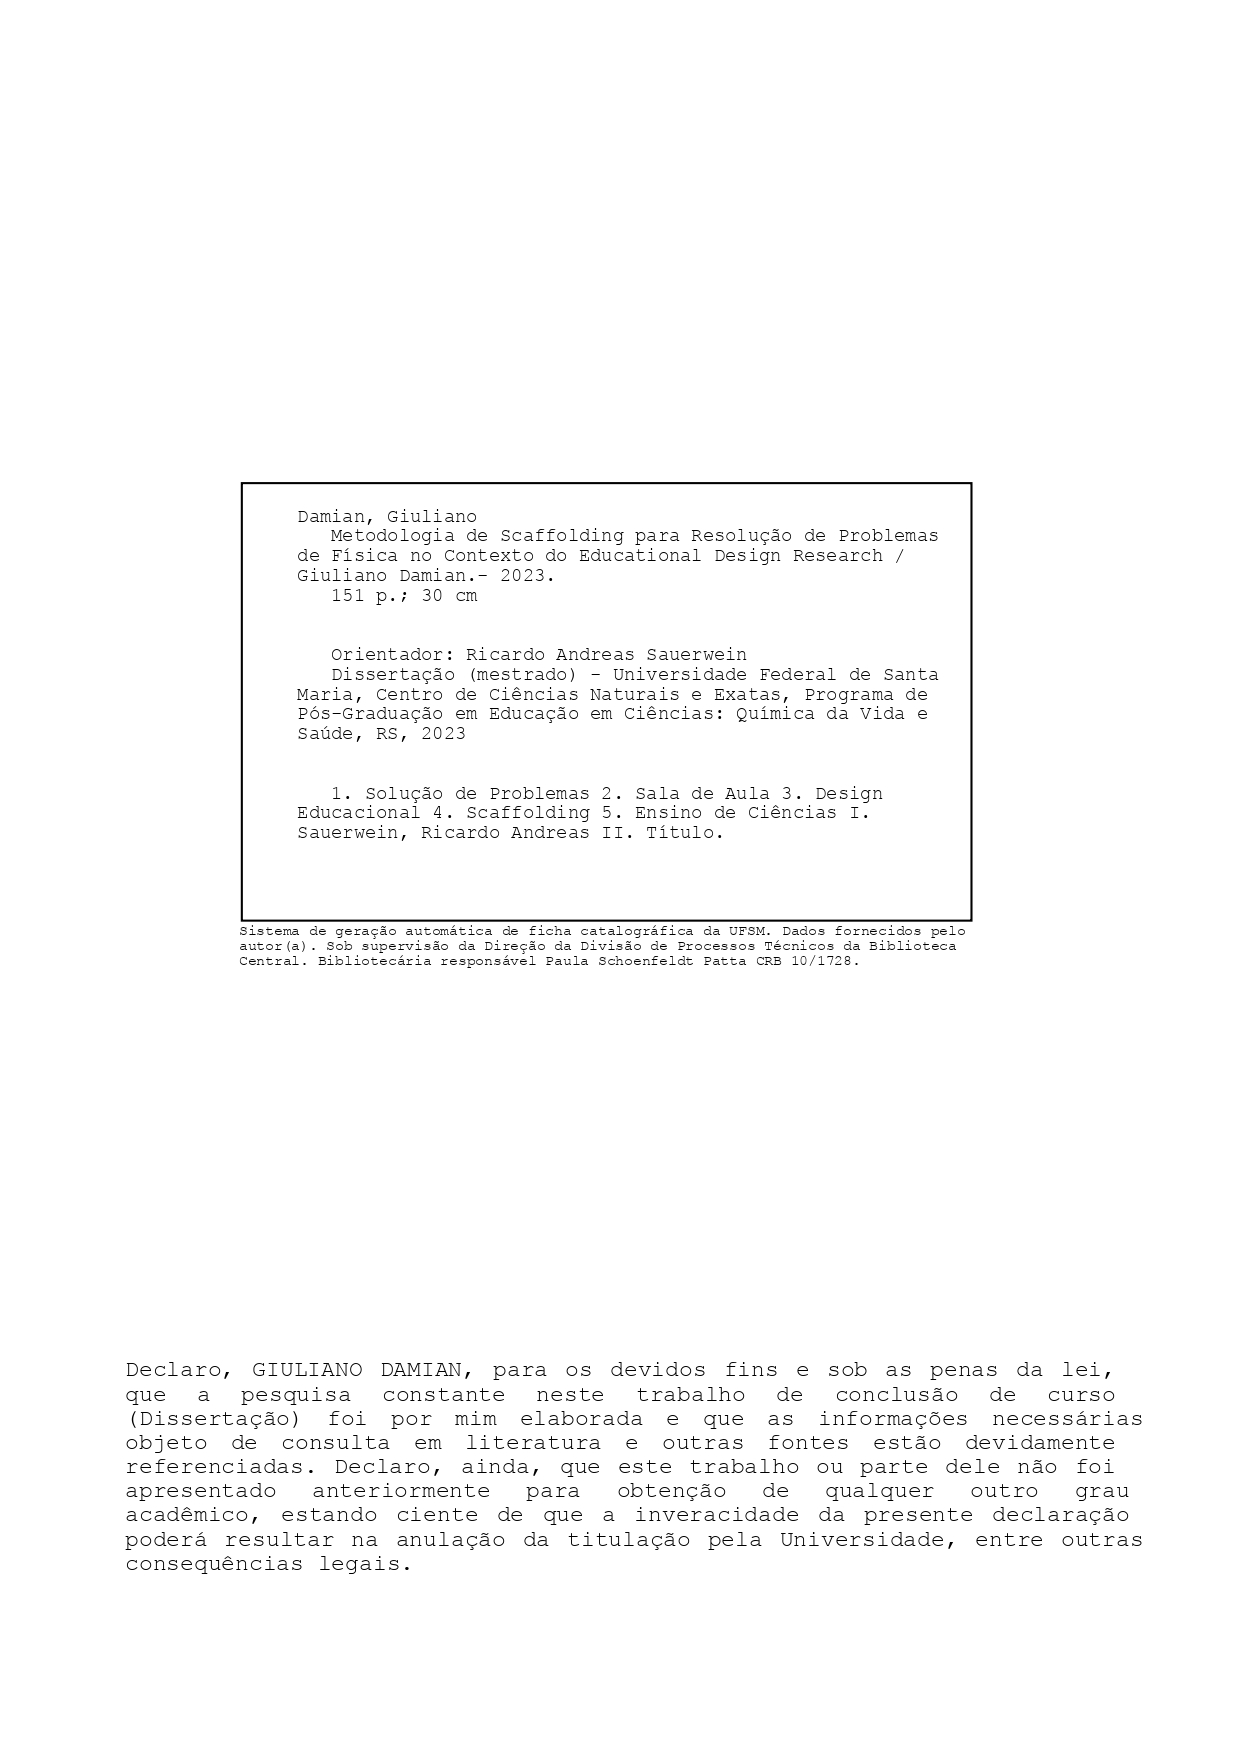
\includegraphics[width=\textwidth,height=\textheight,keepaspectratio]{fig/fichaCatalografica_page-0001.jpg}
%\end{figure}
%\noindent 2023\\
%Todos os direitos autorais reservados a \imprimirautor. A reprodução de partes ou do todo deste trabalho só poderá ser feita mediante a citação da fonte.\\
%E-mail: fsc.damian@gmail.com
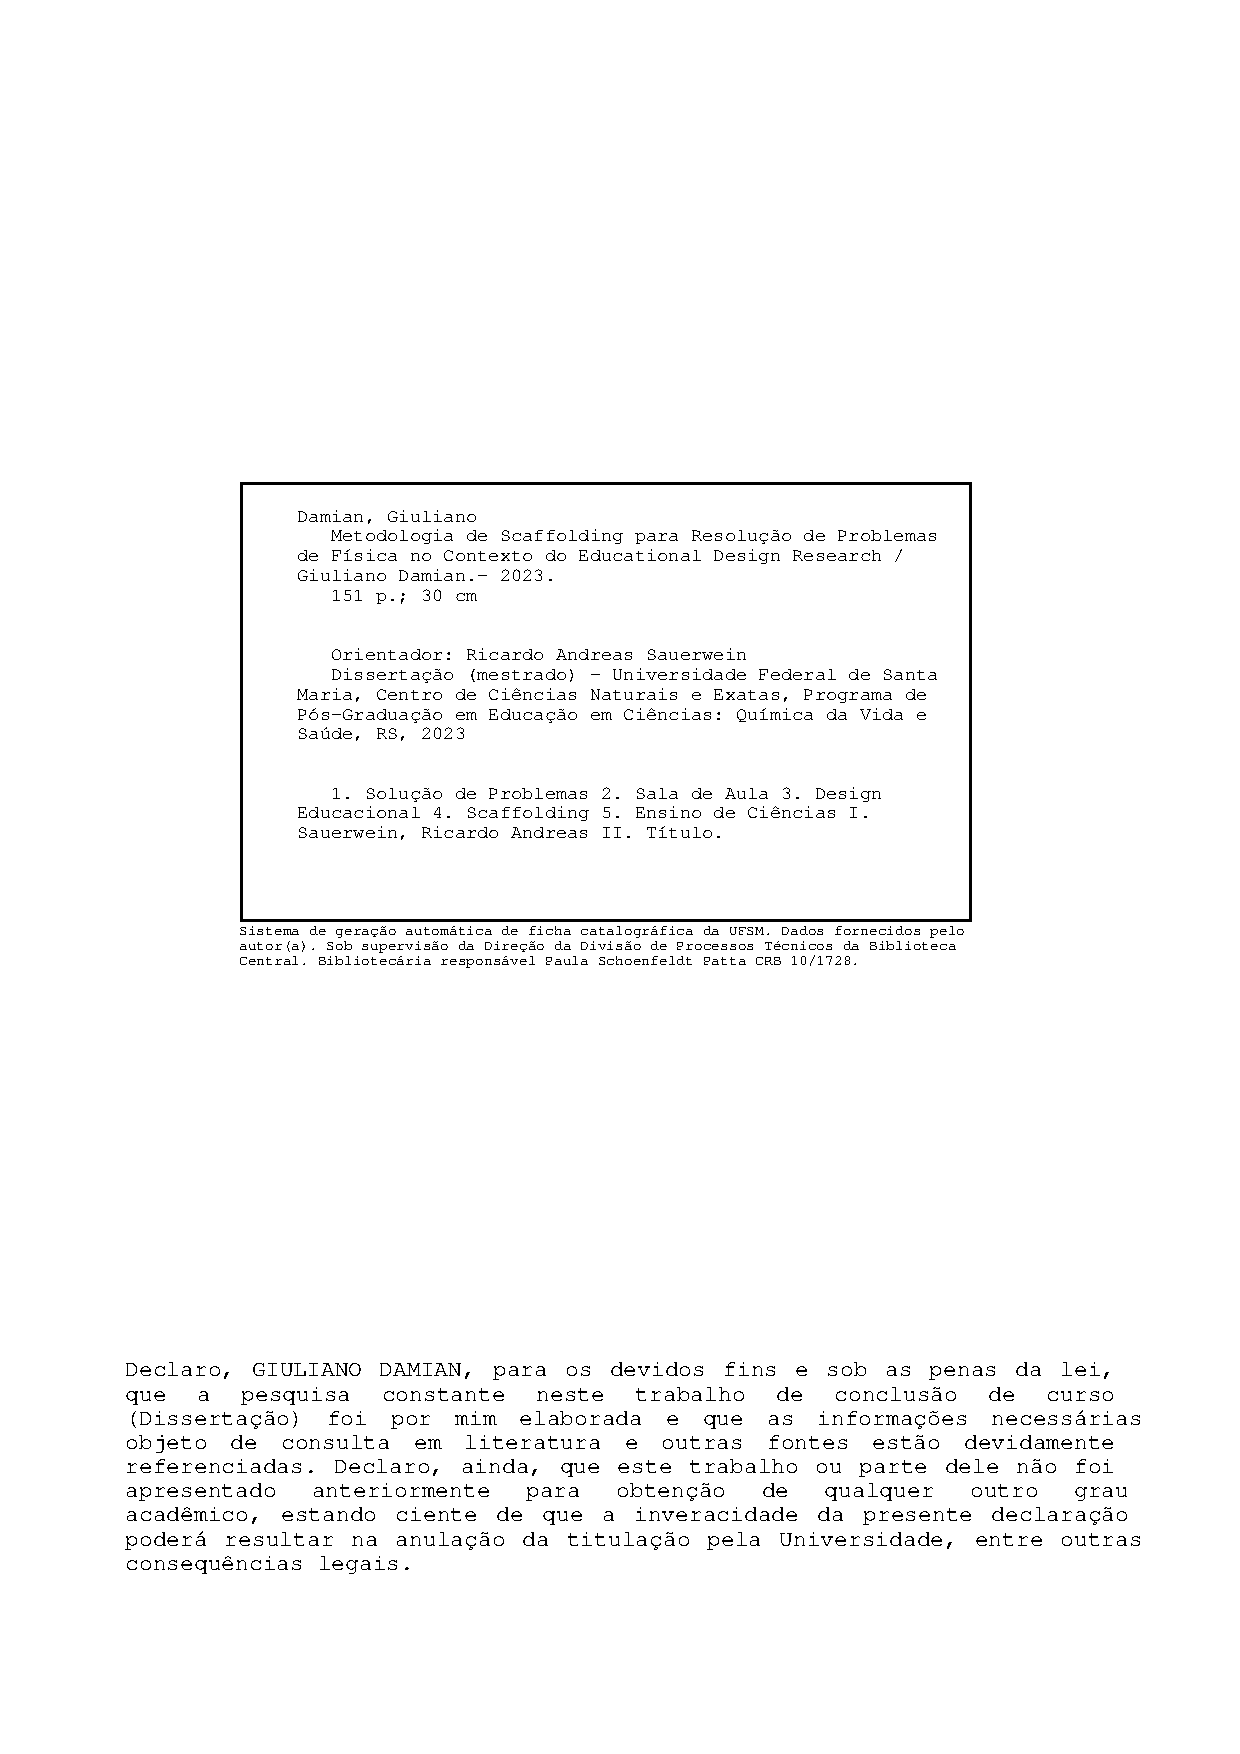
\includepdf[pages=-]{fig/fichaCatalografica.pdf}

\end{fichacatalografica}

% ATENÇÃO!
% Visando atender à exigência da CAPES, conforme Portaria nº 206, de 4 de setembro de
% 2018, 8 deve ser incluída a seguinte nota:
% O presente trabalho foi realizado com apoio da Coordenação de Aperfeiçoamento de Pessoal
% de Nível Superior - Brasil (CAPES) - Código de Financiamento 001
% This study was financed in part by the Coordenação de Aperfeiçoamento de Pessoal de Nível
% Superior - Brasil (CAPES) - Finance Code 001

\begin{folhadeaprovacao}
\center
\begingroup
    \fontsize{12pt}{12pt}\selectfont
    \textbf{\imprimirautor}
\endgroup
\vspace{7em}

\begingroup
    \fontsize{12pt}{12pt}\selectfont
    \textbf{\expandafter\MakeUppercase\expandafter{\imprimirtitulo}}
\endgroup
\vspace{7em}
%
%% Mesmo texto da folha de rosto, mais informações 
%% nas paginas 29 e 30 da MDT. 
%
\begin{flushright}
\begin{minipage}{.50\textwidth}Dissertação apresentada ao Programa de Pós-Graduação em Educação em Ciências da Universidade Federal de Santa Maria (UFSM, RS), como requisito parcial para obtenção do grau de \textbf{Mestre em Educação em Ciências}.
\end{minipage}
\end{flushright}
\vspace{4em}


\textbf{Aprovado em 30 de Agosto de 2023:}
\vspace{48pt}


\makebox[8cm]{\hrulefill}\\
, Dr. Ricardo Andreas Sauerwein (UFSM)\\
(Presidente/Orientador)
\vspace{1.5em}

\makebox[8cm]{\hrulefill}\\

, Dra. Ana Marli Bulegon (UFN)
\vspace{1.5em}

\makebox[8cm]{\hrulefill}\\
, Dr. Dioni Paulo Pastorio (UFRGS)
\vspace{1.5em}

%\makebox[8cm]{\hrulefill}\\

%, Dr. (EXT)
%\vspace{1.5em}

%\makebox[8cm]{\hrulefill}\\
%, Dr. (EXT)

\vfill

\begingroup
    \fontsize{12pt}{12pt}\selectfont
    \imprimirlocal\\
    \imprimirdata
\endgroup

\end{folhadeaprovacao}
 %% MODELO JUNTO AO DOCUMENTO PRINCIPAL
\linespread{1.5}
\begin{dedicatoria}
\vspace*{\fill}
\center{Aos meus pais Vladimir e Albimari, e minha cônjuge Andréa.}
\vspace*{\fill}
\end{dedicatoria}		%% MODELO JUNTO AO DOCUMENTO PRINCIPAL
\begin{agradecimentos}[AGRADECIMENTOS]

Agradeço à Universidade Federal de Santa Maria pelos anos de ensino com profunda gratidão e reconhecimento. Durante essa jornada, fui agraciado com oportunidades únicas de aprendizado, crescimento acadêmico e desenvolvimento pessoal. A dedicação e excelência dos professores e equipe administrativa foram fundamentais para minha formação e para minha evolução como estudante e indivíduo. Além disso, a diversidade de experiências e conhecimentos proporcionados pela universidade ampliou minha visão de mundo e me preparou para enfrentar os desafios futuros. 

Aos membros do grupo Métodos e Processos de Ensino e Aprendizagem de Ciências, sou grato por cada momento compartilhado e por todas as oportunidades de aprendizado proporcionadas. Suas contribuições enriqueceram minha formação acadêmica e pessoal, e sinto-me privilegiado por ter sido parte desse grupo tão comprometido e inspirador. Que a amizade e as experiências vivenciadas permaneçam conosco, impulsionando-nos a seguir na busca por uma educação cada vez mais significativa e transformadora.

À minha família, que sempre esteve ao meu lado, não tenho palavras para descrever o quanto sou grato por todo o amor, paciência e compreensão que vocês me proporcionaram ao longo desta jornada. Vocês foram meu porto seguro nas horas de dúvida e meu maior incentivo para prosseguir quando o cansaço se fazia presente. Cada palavra de encorajamento e gesto de carinho foi essencial para que eu mantivesse o foco e a determinação em alcançar este objetivo.

Aos meus amigos, que estiveram ao meu lado nas horas boas e ruins, saibam que a amizade de vocês foi um verdadeiro alento durante todo esse processo. Cada palavra de ânimo e cada risada compartilhada foram importantes para manter o equilíbrio emocional e a confiança em mim mesmo.

E, aos colegas do Kendo, que compartilham comigo a paixão por esse esporte e os valores de respeito e disciplina, sou grato pela amizade sincera e pelos ensinamentos que ultrapassam as paredes do dojo. Nosso convívio enriqueceu minha vida acadêmica e pessoal, e cada treino foi uma oportunidade de crescimento mútuo.

\end{agradecimentos}		%% MODELO JUNTO AO DOCUMENTO PRINCIPAL
\begin{epigrafe}
\vspace*{\fill}
\begin{flushright}{}


%\begin{minipage}[b]{8cm}

\textit{Todos esses que aí estão\\
Atravancando meu caminho,\\
Eles passarão...\\
Eu passarinho!\\
 (\small{Poeminho do Contra - Mario Quintana })}



%\end{minipage}
\end{flushright}
\end{epigrafe}			%% MODELO JUNTO AO DOCUMENTO PRINCIPAL
\begin{resumo}[RESUMO]
\vspace{2em}
\begin{center}
%se der mais de uma página pode ser escrito em fonte 10pt
\textbf{\expandafter\MakeUppercase\expandafter{\imprimirtitulo}}\\
\vspace{1em}
AUTOR: \imprimirautor\\
ORIENTADOR: \imprimirorientador
\end{center}
\vspace{1em}
% texto
Este trabalho tem como foco o estudo da competência de Resolução de Problemas (RP) no contexto da área de Física, utilizando a metodologia de \textit{Scaffolding}. Para alcançar esse objetivo, adotamos a abordagem metodológica do \textit{Educational Design Research} para orientar nossas atividades de pesquisa. As aplicações em sala de aula foram realizadas por meio de dois modelos principais: Oficinas de Resolução de Problemas (ORP) e Atividades de Sala de Aula (ASA). O estudo contou com três aplicações de ORP em turmas do Ensino Superior, bem como três aplicações de ASA em turmas do Ensino Médio. As ORP e ASA foram complementares, interligando-se através de processos de \textit{redesign}, que foram gerados para atender às necessidades que surgiram ao longo das aplicações. Os objetivos da pesquisa estão claramente delineados, com enfoque na avaliação da eficácia da metodologia de \textit{Scaffolding} em relação à competência de Resolução de Problemas, tanto em cada aplicação específica como de forma geral.

\vspace{2em}
%no minimo tres separadas por .
\textbf{Palavras-chave}: Solução de Problemas. \textit{Feedback}. Sala de Aula. \textit{Redesign} Educacional. Ensino de Ciências.
\end{resumo}				%% MODELO JUNTO AO DOCUMENTO PRINCIPAL
\begin{resumo}[ABSTRACT]
\vspace{2em}
\begin{center}
%se der mais de uma página pode ser escrito em fonte 10pt

\textbf{\expandafter\MakeUppercase\expandafter{\imprimirtituloestrangeiro}}\\
AUTHOR: \imprimirautor\\
ADVISOR: \imprimirorientador
\end{center}
\vspace{1em}
% texto
This dissertation focuses on studying the competence of Problem-Solving in the context of Physics, utilizing the methodology of Scaffolding. To achieve this objective, the Educational Design Research approach was adopted to guide the research activities. The applications in the classroom were carried out using two main models: Problem-Solving Workshops and Classroom Activities. The study included three applications of Problem-Solving Workshops in Higher Education classes and three applications of Classroom Activities in High School classes. The Problem-Solving Workshops and Classroom Activities were complementary, interconnected through redesign processes, which were generated to address emerging needs throughout the applications. The research objectives are clearly delineated, with a focus on evaluating the effectiveness of the Scaffolding methodology concerning the competence of Problem-Solving, both in each specific application and overall.

\vspace{2em}
%no minimo tres separadas por .
\textbf{Keywords}: Problem-Solving. Feedback. Classroom. Educational Redesign. Science Education.
\end{resumo}			%% MODELO JUNTO AO DOCUMENTO PRINCIPAL
\listoffigures*	%% O * retira listas do sumario 
\cleardoublepage
\listoftables*
\cleardoublepage
\begin{siglas}
    \item[ASA] Atividades de Sala de Aula 
    \item[ASA1] Primeira aplicação da ASA 
    \item[ASA2] Segunda aplicação da ASA 
    \item[ASA3] Terceira aplicação da ASA 
    \item[CN] Ciências da Natureza
    \item[EDR] \textit{Educacional Design Research}
    \item[MPEAC] Métodos e Processos de Ensino e Aprendizagem de Ciências
    \item[ORP] Oficinas de Resolução de Problemas
    \item[ORP1] Primeira aplicação da ORP
    \item[ORP2] Segunda aplicação da ORP
    \item[ORP3] Terceira aplicação da ORP
    \item[RP] Resolução de Problemas
    \item[SBC] \textit{Scaffolding} Baseado em Computadores
    \item[SPP] \textit{Scaffolding} por Pares
    \item[SUU] \textit{Scaffolding} Um a Um
    \item[UFSM] Universidade Federal de Santa Maria
 
    % Adicione mais siglas conforme necessário
\end{siglas}
\cleardoublepage
\tableofcontents*	%% imprime sumario
\clearpage			%% retira numeração de pagina do sumario
\textual
%
%% TEXTO
%
\chapter{Introdução}\label{ch:intro}

\section{Estrutura da Dissertação}

O presente trabalho é organizado em sete capítulos. No Capítulo \ref{ch:intro}, são expostas as fundamentações que motivaram a elaboração desta dissertação, além dos objetivos delineados para a pesquisa.

No Capítulo \ref{ch:edr}, abordamos os conceitos fundamentais da nossa abordagem de pesquisa, o \textit{Educational Design Research} (EDR). Nesse capítulo, enfatizamos os aspectos essenciais dessa concepção, bem como a perspectiva adotada pelo nosso grupo de pesquisa - Métodos e processos de Ensino e Aprendizagem (MPEAC).

No Capítulo \ref{ch:rp}, serão discutidos os principais aspectos da Resolução de Problemas (RP), que é o foco central desta dissertação. Nessa seção, serão abordados os fundamentos teóricos e práticos relacionados à abordagem de RP e sua relevância para o desenvolvimento da pesquisa.

No Capítulo \ref{ch:schaffolding}, será realizada uma análise detalhada da metodologia de \textit{Scaffolding}, que serve como base para esta dissertação. É importante ressaltar que os conteúdos abordados nos Capítulos \ref{ch:edr}, \ref{ch:rp} e \ref{ch:schaffolding} constituem os três pilares fundamentais para a implementação desta pesquisa.

No Capítulo \ref{ch:apl}, discutiremos como foram concebidas as Oficinas de Resolução de Problemas (ORP) e as Atividades de Sala de Aula (ASA). Todo esse processo foi pensado e desenvolvido visando analisar a competência de RP em Física e explorar a metodologia de \textit{Scaffolding} como uma ferramenta de apoio ao aprendizado dos alunos.

No Capítulo \ref{ch:resanddisc}, procedemos com uma análise detalhada e individual de cada ORP e ASA. Dessa forma, visando correlacionar os resultados obtidos com os objetivos específicos deste estudo. 

No Capítulo \ref{ch:conclusao}, apresentamos nossas considerações finais sobre a metodologia de \textit{Scaffolding}. Neste capítulo, abordamos a resposta ao objetivo geral da pesquisa, bem como fornecemos uma análise mais ampla dos objetivos específicos. Além disso, oferecemos sugestões para futuras pesquisas e possíveis desdobramentos do estudo.

\section{Justificativa}

 Após diálogos no grupo MPEAC, foi constatado que os alunos apresentam dificuldades na resolução de problemas de Física, persistindo desde o Ensino Fundamental até a primeira metade do ensino superior. Essas dificuldades se mostram como um desafio a ser superado no processo de aprendizagem.
 
A dificuldade na resolução de problemas apresenta uma preocupação relevante para a formação de futuros profissionais, uma vez que interfere na habilidade de interpretar situações-problema e elaborar estratégias de resolução. Durante o desenvolvimento deste trabalho, será demonstrado que a existência de lacunas em outras áreas de ensino, principalmente em Matemática, contribui para a intensificação das dificuldades dos alunos. 

A resolução de problemas é uma preocupação que engloba tanto os resultados quanto o processo de desenvolvimento. É fundamental considerá-la como uma etapa essencial no processo de ensino-aprendizagem de Física, uma vez que por meio dela os alunos tem seus conhecimentos conceituais e atitudinais postos à prova e são desafiados a aplicá-los de forma prática.

\citeonline{lurdes2018}, \citeonline{silva2019} e \citeonline{oliveira2017} discutem os desafios da Resolução de Problemas em Física. Além disso, de forma geral, concordam que as dificuldades no processo de resolução, apesar de ser algo amplamente estudado \cite{oliveira2017}, persistem até os dias atuais.


Com efeito, a resolução de um problema requer uma motivação inicial, seguida por uma análise cuidadosa da situação-problema e, por fim, a elaboração e execução de um plano de resolução. Essa sequência de passos é fundamental para o processo efetivo de solução de problemas em qualquer contexto, inclusive no ensino e aprendizagem de Física.

Frequentemente, os estudantes encaram as dificuldades nos problemas como obstáculos insuperáveis, o que pode desmotivá-los a prosseguir no processo de resolução. Nesse contexto, acreditamos que é papel do professor auxiliar o aluno durante essa etapa crucial de aprendizagem, oferecendo suporte e orientação para ajudá-los a superar tais barreiras e aprimorar suas habilidades de resolução de problemas.

Poderíamos mencionar diversas abordagens que permitem ao professor auxiliar os alunos nos processos de resolução de problemas, mas neste trabalho, focalizaremos a metodologia de \textit{Scaffolding}. Em um estudo de \citeonline{wood1976} explorou esse processo de tutoria com grupos de crianças, buscando desenvolver, entre outros efeitos, suas habilidades motoras. Neste contexto, nosso objetivo é investigar essa abordagem como forma de auxiliar os estudantes na resolução de problemas de Física.

O método de \textit{Scaffolding} foi selecionado por sua aplicabilidade em diversos contextos e por oferecer diferentes formas de utilização, além de possuir uma implementação simples e facilmente compreensível pelos alunos. Essa abordagem consiste no fornecimento de "andaimes" (tradução do inglês "\textit{Scaffolds}"), que servem de suporte para o desenvolvimento do processo de resolução de problemas.

De fato, assim como os andaimes temporários empregados em construções, as dicas utilizadas na metodologia de \textit{Scaffolding} não são permanentes. Elas têm a função de auxiliar o aluno no processo de resolução de problemas, sendo gradativamente removidas à medida que o estudante adquire as habilidades e conhecimentos necessários para solucionar o problema de forma autônoma e completa. O propósito é promover a capacidade do aluno de aplicar o aprendizado adquirido de maneira efetiva e sustentada.

Com base nessa perspectiva, acreditamos que um \textit{Scaffolding} bem estruturado e aplicado adequadamente possa auxiliar o aluno a superar dificuldades e avançar em sua resolução de problemas. Ao fornecer um suporte estratégico e personalizado, o \textit{Scaffolding} pode capacitar os estudantes a enfrentarem desafios com maior confiança e sucesso, estimulando o desenvolvimento de suas habilidades cognitivas e metacognitivas.

Nossa abordagem de pesquisa segue o gênero \textit{Educational Design Research}, que se caracteriza pela aplicação contínua de investigações educacionais, permitindo, se necessário, um \textit{redesign} e uma subsequente reaplicação, com o objetivo de buscar aprimorar os resultados alcançados. Essa metodologia permite uma abordagem iterativa e adaptativa, buscando constantemente a melhoria do processo de ensino-aprendizagem e o desenvolvimento de estratégias mais efetivas para a resolução de problemas em Física.

Essa dissertação se apoia em três pilares fundamentais: a Resolução de Problemas em Física, a abordagem de pesquisa EDR e a metodologia de \textit{Scaffolding}. Através da aplicação do método de \textit{Scaffolding} para a Resolução de Problemas de Física, sob a perspectiva do EDR, buscamos compreender a efetividade dessa abordagem na promoção do desenvolvimento da competência de resolução de problemas dos alunos. Ao adotar o EDR, visamos aprimorar a metodologia de ensino e aprendizagem, identificando possíveis ajustes e otimizações ao longo do processo, com o objetivo de aprimorar os resultados e proporcionar uma melhor experiência de aprendizado para os estudantes.

\section{Objetivos}

Com o objetivo de orientar esta investigação, foram formulados um objetivo geral e cinco objetivos secundários para esta dissertação.

\textbf{Objetivo geral}: Verificar se a metodologia do \textit{Scaffolding} consegue contribuir para o desenvolvimento da competência da resolução de problemas em Física.

 
\textbf{Objetivos Secundários:}

\begin{enumerate}[label=\alph*)]
    \item \label{item:a} Compreender como os alunos resolvem os problemas de Física; 
    \item \label{item:b} Quais etapas da resolução de problemas demandam mais auxílio; 
    \item  \label{item:c} Verificar a evolução temporal das resoluções dos problemas; 
    \item \label{item:d} Quais formas de ajuda são mais eficientes para a compreensão dos alunos;
    \item \label{item:e} O interesse na resolução dos problemas se mantém ao longo do semestre.
\end{enumerate}
\chapter{Concepção de pesquisa através do \textit{Educational Design Research}} \label{ch:edr}

O \textit{Educational Design Research} (EDR) é uma abordagem metodológica que visa integrar a teoria e a prática para desenvolver soluções eficazes e inovadoras em contextos educacionais. A essência do EDR reside no reconhecimento de que os desafios enfrentados por organizações e comunidades educacionais são complexos e multifacetados, indo além de meros problemas teóricos e demandando soluções práticas que atendam às necessidades reais.

Essa abordagem enfatiza uma perspectiva holística, ou seja, a compreensão dos problemas educacionais deve considerar os diferentes aspectos e contextos envolvidos. A colaboração entre pesquisadores e partes interessadas é valorizada, uma vez que essas últimas trazem consigo experiências práticas, percepções e conhecimentos do mundo real, complementando as visões teóricas dos pesquisadores. A sinergia resultante entre teoria e prática é fundamental para o desenvolvimento de soluções que possam ser efetivamente implementadas e que produzam impactos significativos no ambiente educacional.

Na Seção \ref{ch:edrtrue} faremos um apanhado geral sobre o EDR que foi o método de pesquisa abordado nesta dissertação. Por fim, na Seção \ref{ch:edrmpeac} faremos uma breve descrição das concepções do EDR do ponto de vista do nosso gurpo de pesquisa: Métodos e Processos de Ensino e Aprendizagem de Ciências (MPEAC).

\section{\textit{Educational Design Research}} \label{ch:edrtrue}

De acordo com \citeonline[p.326]{McKenney2018}, o EDR é caracterizado por seu compromisso em conjuntamente desenvolver percepções teóricas e soluções práticas em contextos reais, em colaboração com as partes interessadas. Este método se distingue das demais abordagens de pesquisa científica ao buscar uma abordagem integrada e aplicada, onde a teoria e a prática são desenvolvidas de forma simultânea e complementar, resultando em soluções eficazes e relevantes para as questões reais enfrentadas pela comunidade de interesse.

O uso do EDR proporciona uma análise detalhada e abrangente de diversas formas de soluções no contexto educacional, englobando processos, programas, políticas e produtos educacionais. Conforme ressaltado por \citeonline{McKenney2018}, o EDR oferece uma abordagem flexível e adaptável, permitindo que os pesquisadores se concentrem em diferentes aspectos do cenário educacional, de acordo com suas necessidades e objetivos específicos de pesquisa.

Ao adotar o EDR como metodologia de pesquisa, os investigadores tem a oportunidade de explorar e descrever a concepção, desenvolvimento, implementação e avaliação de soluções educacionais com uma perspectiva mais integrada, conforme destacado por \citeonline{plomp2013educational}. Essa abordagem possibilita uma visão mais completa e aprofundada dos desafios enfrentados e das possíveis maneiras de superá-los.

Um aspecto relevante do EDR é a sua aplicação em projetos de intervenção, nos quais programas e práticas educacionais são desenvolvidos e testados em contextos reais. Esse enfoque permite uma investigação profunda das soluções propostas, incluindo sua viabilidade, eficácia e impacto nos resultados de aprendizagem dos alunos, bem como na dinâmica da sala de aula e na experiência do professor.

Outro campo de estudo abarcado pelo EDR é a análise de políticas educacionais, identificando seus pontos fortes, desafios e impactos em nível macro nas instituições de ensino e na sociedade em geral. Isso inclui a investigação das políticas de inclusão, avaliação educacional, formação de professores, entre outras, contribuindo para a compreensão dos resultados e aprimoramento das melhores práticas.

Além disso, a abordagem do EDR também pode ser aplicada na análise de produtos educacionais, como softwares, aplicativos, recursos didáticos e materiais instrucionais. Ao adotar essa perspectiva, os pesquisadores podem avaliar a usabilidade, eficácia e adequação desses produtos para apoiar o processo de ensino e aprendizagem, conforme mencionado por \citeonline{anderson2012design}.

É importante enfatizar que o EDR abrange várias variações e abordagens específicas, de acordo com as áreas de estudo e as demandas de pesquisa. No entanto, em um contexto geral, o EDR oferece uma perspectiva integradora e colaborativa, na qual pesquisadores, educadores e demais partes interessadas trabalham juntos para desenvolver soluções mais eficazes e adaptadas ao contexto educacional. Ao fazer isso, o EDR contribui para o avanço da pesquisa educacional e para a melhoria contínua da qualidade da educação.

Dizemos que o EDR é definido como um tipo de pesquisa que emprega o desenvolvimento iterativo de soluções para abordar problemas educacionais práticos e complexos, permitindo uma investigação empírica que resulta em uma compreensão teórica que pode informar o trabalho de outros pesquisadores \cite[p.326]{McKenney2018}. Os objetivos e métodos do EDR estão estreitamente alinhados com o mundo real e suas várias facetas.

O EDR se preocupa em desenvolver o que \citeonline{Legemann2002} denominou de conhecimento utilizável, tornando os resultados da pesquisa relevantes para a prática educacional. Esse conhecimento útil é produzido ao longo da pesquisa e é fundamentalmente importante compartilhá-lo com outros pesquisadores e profissionais, destacando a importância da troca de informações para o progresso e desenvolvimento teórico na área.

Essa abordagem de pesquisa, com base no desenvolvimento iterativo de soluções e uma investigação empírica, contribui para a produção de conhecimentos aplicáveis e pertinentes ao contexto educacional, favorecendo uma interação contínua entre a teoria e a prática.

De acordo com \citeonline[p.5]{DBRC2003}, uma boa pesquisa baseada em \textit{design} deve apresentar cinco importantes características. A primeira é a interligação entre os objetivos principais do \textit{design} de ambientes de aprendizagem e o desenvolvimento de teorias ou protótipos de aprendizagem. Segundo \citeonline{DBRC2003}, essa integração permite que as soluções educacionais propostas sejam fundamentadas em bases teóricas sólidas.

A segunda característica ressaltada por \citeonline{DBRC2003} é que o desenvolvimento e a pesquisa devem ocorrer em etapas cíclicas e contínuas de projeto, execução, análise e redesenho. Esse processo iterativo permite ajustes e melhorias contínuas nas intervenções educacionais, de acordo com os resultados obtidos.

Em terceiro lugar, \citeonline{DBRC2003} enfatizam que a pesquisa baseada em \textit{design} deve levar a teorias compartilháveis que possam auxiliar outros pesquisadores da área. Essa colaboração e disseminação do conhecimento contribuem para o avanço da comunidade acadêmica e para o crescimento do campo educacional, conforme mencionado por \citeonline{Collins1992} e \citeonline{Coob2001}.

A quarta característica destacada por \citeonline{DBRC2003} ressalta a importância de documentar detalhadamente como o \textit{design} funciona em ambientes reais de aprendizagem. Isso inclui não apenas relatar o sucesso ou fracasso da intervenção, mas também descrever as interações e processos envolvidos na compreensão das questões de aprendizagem.

Por fim, a quinta característica ressaltada por \citeonline{DBRC2003} é que o desenvolvimento da pesquisa deve se basear em métodos que possam documentar desde a concepção e implementação do \textit{design} até a análise dos resultados alcançados. Essa abordagem metodológica rigorosa garante a robustez e a confiabilidade da pesquisa baseada em \textit{design}. 

Ainda, segundo o \citeonline[p.5]{DBRC2003}: 

\begin{quoting} 
[leftmargin=4cm, rightmargin=0cm]
\noindent
É importante ressaltar que a pesquisa baseada em design vai além do mero projeto e teste de intervenções específicas. As intervenções incorporam afirmações teóricas específicas sobre o ensino e aprendizagem, e refletem um compromisso com a compreensão das relações entre teoria, projeto de produtos, e prática. Ao mesmo tempo, pesquisas sobre intervenções específicas podem contribuir para teorias de aprendizagem e ensino.
\end{quoting}

Os resultados obtidos através do EDR são cuidadosamente analisados e discutidos, permitindo que ocorra uma reaplicação das soluções, incorporando as modificações e aprimoramentos necessários. Esse processo iterativo é fundamental para a melhoria contínua das intervenções e para o aperfeiçoamento das soluções propostas ao longo do tempo.

É essencial que todo o processo de pesquisa seja documentado de forma rigorosa e clara. A documentação permite que outros pesquisadores compreendam detalhadamente o estudo realizado, possam replicá-lo e adaptá-lo para suas próprias realidades e contextos educacionais.

O compartilhamento dos resultados e das experiências é um aspecto crucial do EDR. Ao disponibilizar as descobertas, lições aprendidas e as soluções desenvolvidas, a comunidade acadêmica e os profissionais da educação podem se beneficiar das contribuições uns dos outros, enriquecendo o conhecimento coletivo e promovendo avanços no campo educacional.

Portanto, o EDR é um processo cíclico e colaborativo, onde a pesquisa, o \textit{design}, a implementação, a análise e a documentação são partes essenciais. Através desse enfoque, o EDR visa gerar e compartilhar conhecimento aplicado que contribua para o aprimoramento contínuo da educação e para o benefício da sociedade como um todo. A Figura \ref{fig:mattaeboa} representa, de forma esquemática, o processo cíclico do EDR.

\begin{figure}[H]
\caption{Processo cíclico do EDR.}
  \label{fig:mattaeboa}
  \centering
  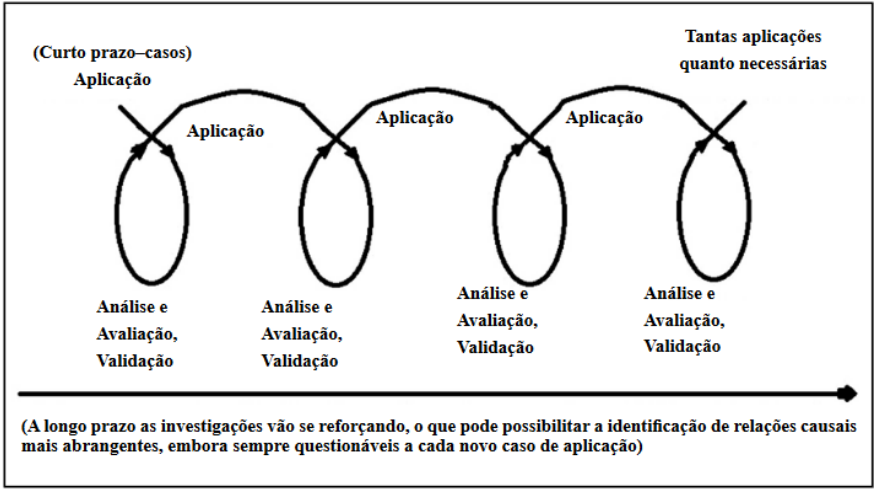
\includegraphics[width=0.8\textwidth]{fig/mattaeboa.png}
  \caption*{Fonte: Retirado de \citeonline[p.29]{MATTA2014}.}
\end{figure}

Resumidamente, segundo \cite{alves2018}, \cite{MATTA2014} e \cite{McKenney2018}, o EDR destaca-se das demais modalidades de investigação nas áreas de Educação ou Ensino devido a um conjunto específico de características distintivas. Estas incluem sua abordagem teoricamente orientada, seu caráter intervencionista, a ênfase na colaboração, a capacidade de resposta às necessidades contextuais e o processo iterativo. 

\begin{table}[H]
\centering
\caption{Características do EDR} \label{tab:carctEDR}
\begin{tabular}{p{5.8cm} p{6.7cm}}
\hline 
\textbf{Teoricamente Orientada} & Constituída a partir dos princípios de design já existentes.\\ 
\hline 
\textbf{Intervencionista} & Inclui a implementação do produto criado.\\ 
\hline 
\textbf{Colaborativa} & Pode ser conduzida em diferentes graus de colaboração entre o pesquisador e/ou profissional que atua em um contexto educacional específico.\\ 
\hline 
\textbf{Responsiva} & Suas pesquisas são conduzidas em ambientes complexos e mutáveis ao longo do tempo.\\ 
\hline 
\textbf{Iterativa} & O ciclo de pesquisa evolui continuamente no tempo.\\ 
\hline 
\end{tabular}
\caption*{Fonte: Criação do Autor baseado no texto de \citeonline{alves2018}.}
\end{table}

Essa diversidade de elementos torna o EDR uma abordagem singular e eficaz na abordagem e solução de questões práticas enfrentadas em contextos educacionais. Na Tabela \ref{tab:carctEDR} apresentamos as características presentes no EDR, de forma resumida.

\section{EDR no MPEAC} \label{ch:edrmpeac}

Na perspectiva do grupo de pesquisa MPEAC, a ênfase reside no desenvolvimento de uma solução aplicada para um problema real e específico \cite{alves2018}. Além disso, há um comprometimento com a efetiva implementação e sustentação das soluções já concebidas.

\begin{table}[H]
\ABNTEXfontereduzida % Reduzir tamanho da fonte conforme normas ABNT
\centering % Centralizar a tabela
\caption{Etapas do EDR no MPEAC}
\label{tab:etapas-edr-mpeac}
\begin{tabularx}{\linewidth}{@{}lX@{}} % Definir a largura das colunas
\toprule
\textbf{1)} & Identificar/definir uma problemática educacional real e localizada em um contexto concreto de ensino e aprendizagem.\\
\midrule
\textbf{2)} & Especificar uma possível solução para a problemática delimitada anteriormente.\\
\midrule
\textbf{3)} & Desenvolver uma possível solução de acordo com a especificação elaborada na etapa anterior.\\
\midrule
\textbf{4)} & Implementar na prática a solução desenvolvida na etapa anterior.\\
\midrule
\textbf{5)} & Analisar a implementação da solução proposta com vistas ao seu aperfeiçoamento/viabilidade e buscar contribuições teóricas para a área de ensino.\\
\midrule
\textbf{6)} & Observar fenômenos de ensino e aprendizagem com vistas a contribuir para o conhecimento teórico da área.\\
\bottomrule
\end{tabularx}
\source{Adaptado de \citeonline[p. 48]{alves2018}.} % Fonte da tabela
\end{table}

A Tabela \ref{tab:etapas-edr-mpeac} apresenta as etapas do EDR de acordo com a perspectiva do grupo de pesquisa, conforme descrito por \citeonline{alves2018}. Essas etapas representam um processo metodológico sistemático para a concepção, implementação e análise de intervenções educacionais, visando aprimorar o processo de ensino e aprendizagem de forma embasada e estruturada.

A primeira etapa consiste na identificação e definição de uma problemática educacional real e contextualizada. Nessa fase, os pesquisadores buscam compreender os desafios e as necessidades enfrentadas em um ambiente de ensino específico, a fim de delimitar o escopo da pesquisa e estabelecer os objetivos a serem alcançados.

Em seguida, na segunda etapa, é especificada uma possível solução para a problemática identificada. Essa etapa envolve a proposição de estratégias e abordagens que possam ser aplicadas de forma concreta para enfrentar o problema educacional em questão.

Na terceira etapa, acontece o desenvolvimento da solução proposta, transformando-a em um plano prático. Nesse estágio, os pesquisadores detalham e elaboram as intervenções educacionais com base nas especificações previamente definidas.

A implementação da solução ocorre na quarta etapa, na qual as intervenções educacionais são colocadas em prática em um ambiente real de ensino e aprendizagem. Durante essa fase, os pesquisadores podem ajustar e adaptar a intervenção de acordo com as necessidades e desafios identificados na execução.

Na quinta etapa, os pesquisadores analisam criticamente a implementação da solução, buscando identificar pontos fortes, fraquezas e oportunidades de melhoria. Essa análise detalhada visa aperfeiçoar a intervenção e, ao mesmo tempo, contribuir para o avanço do conhecimento teórico na área de ensino e aprendizagem.

Por fim, na sexta etapa, a observação de fenômenos de ensino e aprendizagem busca oferecer uma contribuição valiosa para o conhecimento teórico no campo educacional. Essa etapa visa ampliar a compreensão dos processos educacionais envolvidos na intervenção e, potencialmente, propor teorias ou modelos que possam ser aplicados em outros contextos educacionais.

As etapas do EDR no MPEAC são concebidas como um ciclo iterativo (Figura \ref{fig:mattaeboa}), no qual as aprendizagens e descobertas obtidas em cada fase contribuem para aprimorar as etapas subsequentes. Esse processo dinâmico de investigação permite uma abordagem holística para a resolução de problemas educacionais complexos, promovendo a conexão entre teoria e prática para o avanço da educação.

\chapter{Resolução de Problemas}\label{ch:rp}

Neste trabalho, utilizamos a Resolução de Problemas como estratégia didática para promover o ensino-aprendizagem. Dessa maneira, é de fundamental importância fazermos uma discussão acerca da referida temática (RP). Nesse contexto, uma vez que a definição de problema é polissêmica (ou seja, pode ter diferentes definições a depender do contexto), realizaremos uma discussão no sentido de definir o significado de problema no âmbito do presente trabalho. 

De acordo com \citeonline[p.15]{Echeverria1998} e \citeonline{Lester1983}: que traz uma definição mais tradicional do termo problema poderia ser identificado como “uma situação que um indivíduo ou um grupo quer ou precisa resolver e para a qual não dispõe de um caminho rápido e direto que leve à solução". 

Além da noção de problema, precisamos entender o conceito de exercício que poderia ser identificado como uma situação em que um indivíduo ou grupo de indivíduos quer ou precisa resolver e, para isso, dispõe de um caminho rápido e direto que leva à solução. Ou seja, enquanto um problema apresenta uma novidade do ponto de vista de sua solução, o exercício, por sua vez, é uma repetição de habilidades ou técnicas sobre aprendidas \cite{Echeverria1998}. Como veremos, essa diferença nos conceitos de problema e exercício pode parecer confusa em um primeiro momento, mas compreender essa relação é essencial no emprego da RP como estratégia didática. 

\section{A IMPORTÂNCIA DA DISCUSSÃO ENTRE PROBLEMA E EXERCÍCIO NA PRÁTICA PEDAGÓGICA}

Segundo o que discutimos anteriormente, temos diferenças nos conceitos de problema e exercício, e é muito importante (do ponto de vista pedagógico) saber diferenciá-los. O exercício possui um algoritmo de solução, onde se treina a destreza do aluno, que faz com que a aprendizagem seja mecânica. Tão importante quanto entender esses conceitos é compreender que ambos constituem diferentes tipos de estratégias didáticas e que possuem finalidades didáticas diferentes. 

Apesar de termos uma classificação para os termos problema e exercício, não temos como definir, de forma geral, se determinada atividade é um ou outro. Isso ocorre devido ao fato de que a classificação em problema ou exercício depende de quem vai tentar solucioná-lo. Ou seja, uma determinada atividade pode ser um exercício para o professor, mas um problema para o aluno. Além disso, um problema que seja repetido várias vezes por uma pessoa pode passar a ser um simples exercício, pois ela já identificou os meios de solução e dominou o método. Ou seja, essa mudança da definição de uma atividade como problema ou exercício depende de cada pessoa. 

Assim, como conclui \citeonline[p.17]{Echeverria1998}: “a solução de problemas e a realização de exercícios constituem um continuum educacional cujos limites nem sempre são fáceis de estabelecer”. 

\section{CONTEÚDOS NA RESOLUÇÃO DE PROBLEMAS}

A RP constitui uma importante estratégia didática para o entendimento dos conteúdos, tanto na educação básica quanto na educação superior. Precisamos compreender que quando ensinamos os alunos a resolver problemas estamos, também, ensinando-os a desenvolver certos conteúdos, sejam eles atitudinais, conceituais ou procedimentais, e estratégias que poderão ser reproduzíveis e aplicáveis em novos contextos. Essa característica faz com que a RP seja aplicável na maioria das áreas de conhecimento. 

Quando pensamos em RP, tradicionalmente pensamos no ensino de Matemática. Porém, podemos trabalhar a RP em diferentes contextos, como nas Ciências Naturais ou até mesmo nas Ciências Sociais. Precisamos, portanto, estar cientes da existência dos diversos tipos de classificação para os problemas, seja em função da área de conhecimento, do conteúdo, dos tipos de operações envolvidas, ou de outras características \cite{Echeverria1998}. Essas diferenças existem por causa da forma como se estrutura os conceitos nas diferentes áreas e do tipo de conhecimento que é exigido para resolvê-los. Traremos algumas dessas classificações nas próximas seções. 

Para que seja possível ensinar a resolver um problema é necessário que o professor tenha consciência da complexidade dos passos para resolvê-lo. Essa afirmação pode parecer óbvia, porém, quando se domina determinada técnica ou habilidade, é comum que um professor não perceba as dificuldades mais “simples” que o estudante possui. \citeonline{Polya2006}, em seus estudos centrados na resolução de problemas em Matemática, criou uma sequência de etapas que serviriam para esse fim, demonstrados na Tabela \ref{tab:passos}. 

Podemos então resumir as observações de \cite{Polya2006} e dizer que para resolvermos um problema precisamos de quatro etapas: Compreensão do problema, concepção de um plano, execução de um plano e análise da solução \cite{Echeverria1998}. O conteúdo dessas etapas pode variar de acordo com o tipo, a área ou a peculiaridade do problema. Mas essa sequência algorítmica serve muito bem aos nossos propósitos. 

O primeiro passo para a solução de problemas é, portanto, a compreensão do próprio problema. Afinal, para que possamos classificar uma determinada atividade como problema, devemos estar conscientes de que estamos frente uma situação nova, que houve alguma mudança em relação ao caso anterior, ou, ainda, que temos explicações insuficientes para a realização da tarefa \cite{Echeverria1998}. 

Resumidamente, os primeiros passos para a resolução de um problema é a percepção do que já é conhecido pela pessoa e o entendimento das novas informações disponíveis na questão. Se alguma parte desse passo não puder ser desenvolvida, acabamos por ter uma dificuldade a mais para o processo de resolução. Afinal, se não conseguirmos interpretar as informações que nos sãos fornecidas, o avanço para a segunda etapa se torna inviável. Dessa forma, pode ser que seja necessário rever o conteúdo do problema e reestudar os tópicos pertinentes à questão, para que se possa desenvolver uma base de conhecimento suficiente para resolver o problema. 

\begin{comment}
    \begin{center}
\parbox{\textwidth}{%
\captionof{table}{Passos necessária para resolver um problema.}
\label{tab:passos}
\begin{mdframed}
\textbf{Compreender o problema}

(a) Qual é a incógnita? Quais são os dados? 
(b) Qual é a condição? A condição é suficiente para determinar a incógnita? É suficiente? Redundante? Contraditória? 

\textbf{Conceber um plano}

Já encontrou um problema semelhante? Ou já viu o mesmo problema proposto de maneira um pouco diferente? 
Conhece um problema relacionado com este? Conhece algum teorema que possa lhe ser útil? Olhe a incógnita com atenção e tente lembrar um problema que lhe seja familiar ou que tenha a mesma incógnita, ou uma incógnita similar. 
Este é um problema relacionado com o seu e que já foi resolvido. Você poderia utilizá-lo? Poderia usar o seu resultado? Poderia empregar o seu método? Considera que seria necessário introduzir algum elemento auxiliar para poder utilizá-lo? 
Poderia enunciar o problema de outra forma? Poderia apresentá-lo de forma diferente novamente? Refira-se às definições.
Se não pode resolver o problema proposto, tente resolver primeiro algum problema semelhante. Poderia imaginar um problema análogo um pouco mais acessível? Um problema mais geral? Um problema mais específico? Pode resolver uma parte do problema? Considere somente uma parte da condição; descarte a outra parte. Em que medida a incógnita fica agora determinado? De que forma pode variar? Você pode deduzir dos dados algum elemento útil? Pode pensar em outros dados apropriados para determinar à incógnita? Pode mudar a incógnita ou os dados, ou ambos, se necessário, de tal forma que a nova incógnita e os novos dados estejam mais próximos entre si?Empregou todos os dados? Empregou toda a condição? Considerou todas as noções essenciais concernentes ao problema? 

\textbf{Execução do plano }

(a) Ao executar o seu plano de resolução, comprove cada um dos passos. 
(b) Pode ver claramente que o passo é o correto? Pode demonstrá-lo? 

\textbf{Visão retrospectiva}

Pode verificar o resultado? Pode verificar o raciocínio?
Pode obter o resultado de forma diferente? Pode vê-lo com apenas uma olhada? Você pode empregar o resultado ou o método em outro problema? 
\end{mdframed}
\caption*{Fonte: Adaptado de \citeonline{Echeverria1998,Polya2006}.} %
}
\end{center}
\end{comment}

\begin{table}[ht]
\caption{Passos necessários para resolver um problema.}
\label{tab:passos}
\begin{tabularx}{\textwidth}{@{}X@{}}
\toprule
\textbf{Compreender o problema} \\
(a) Qual é a incógnita? Quais são os dados? \\
(b) Qual é a condição? A condição é suficiente para determinar a incógnita? É suficiente? Redundante? Contraditória? \\
\midrule
\textbf{Conceber um plano} \\
Já encontrou um problema semelhante? Ou já viu o mesmo problema proposto de maneira um pouco diferente? \\
Conhece um problema relacionado com este? Conhece algum teorema que possa lhe ser útil? Olhe a incógnita com atenção e tente lembrar um problema que lhe seja familiar ou que tenha a mesma incógnita, ou uma incógnita similar. \\
Este é um problema relacionado com o seu e que já foi resolvido. Você poderia utilizá-lo? Poderia usar o seu resultado? Poderia empregar o seu método? Considera que seria necessário introduzir algum elemento auxiliar para poder utilizá-lo? \\
Poderia enunciar o problema de outra forma? Poderia apresentá-lo de forma diferente novamente? Refira-se às definições. \\
Se não pode resolver o problema proposto, tente resolver primeiro algum problema semelhante. Poderia imaginar um problema análogo um pouco mais acessível? Um problema mais geral? Um problema mais específico? Pode resolver uma parte do problema? Considere somente uma parte da condição; descarte a outra parte. Em que medida a incógnita fica agora determinada? De que forma pode variar? Você pode deduzir dos dados algum elemento útil? Pode pensar em outros dados apropriados para determinar à incógnita? Pode mudar a incógnita ou os dados, ou ambos, se necessário, de tal forma que a nova incógnita e os novos dados estejam mais próximos entre si? \\
Empregou todos os dados? Empregou toda a condição? Considerou todas as noções essenciais concernentes ao problema? \\
\midrule
\textbf{Execução do plano} \\
(a) Ao executar o seu plano de resolução, comprove cada um dos passos. \\
(b) Pode ver claramente que o passo é o correto? Pode demonstrá-lo? \\
\midrule
\textbf{Visão retrospectiva} \\
Pode verificar o resultado? Pode verificar o raciocínio? \\
Pode obter o resultado de forma diferente? Pode vê-lo com apenas uma olhada? Você pode empregar o resultado ou o método em outro problema? \\
\bottomrule
\end{tabularx}
\caption*{Fonte: Adaptado de \citeonline{Echeverria1998,Polya2006}.}
\end{table}



A segunda etapa na resolução de problemas desenvolvida por \cite{Polya2006} é a concepção de um plano de ação. Ou seja, após identificarmos quais as informações previamente conhecidas e as novas informações, é necessário desenvolver uma estratégia para aplicar esses conhecimentos em prol da resolução. Na Tabela \ref{tab:passos} podemos ver diversos tipos de questionamentos que auxiliam na hora de desenvolver um plano. 

Na terceira etapa da resolução de problemas é necessário pôr em prática o plano desenvolvido. Após isso, na quarta etapa, é verificado se o resultado condiz com a pergunta. É de suma importância perceber que as quatro etapas de \citeonline{Polya2006} para a resolução de problemas formam uma sequência bem definida para a resolução. Se uma das etapas não for corretamente executada, acarretará num erro sistemático no restante do processo. Além disso, devemos dar uma atenção especial para o quarto passo. Pois sem ele não seria possível saber se todas as etapas anteriores foram corretamente trabalhadas. 

Podemos citar o fato de que o processo de resolução de problemas de \citeonline{Polya2006} é extremamente linear. Como fora discutido anteriormente, se uma etapa não puder ser concluída, não poderemos seguir adiante com a próxima. Entretanto, a solução de problemas não segue sempre uma sequência linear como estamos descrevendo \cite{Echeverria1998}. Quando introduzimos uma questão para resolver uma etapa do problema, por exemplo, “Considera que seria necessário introduzir algum elemento auxiliar para poder resolver o problema”, acabamos gerando um novo problema que requer que os mesmos quatro passos sejam seguidos. Dessa forma, acabamos por entrar em um loop de RP. 

Ao tentar resolver um problema, a forma de abordar e desenvolver seus passos vai variar de pessoa para pessoa, de acordo com seus conhecimentos prévios e motivações na hora da resolução. Ou seja, mesmo tendo uma “receita” para seguir no processo da RP, cada pessoa pode seguir por caminhos diferentes, utilizando de habilidades e estratégias distintas. Essa diferença se torna mais evidente entre especialistas e principiantes da área do problema em questão. 
\section{ESPECIALISTAS E PRINCIPIANTES NA RP}
Recapitulando, na hora de resolver um determinado problema, pessoas diferentes podem resolver de modos diferentes, mesmo seguindo os passos para RP descritos por \citeonline{Polya2006}. Isso se deve ao fato de que cada uma das pessoas possui uma bagagem de conhecimentos e experiências diferentes, o que pode facilitar ou dificultar o processo de RP. Como critério de classificação, podemos separar as pessoas em dois grupos distintos: os especialistas e os principiantes. 

Antes de qualquer coisa, é preciso ressaltar que a separação e análise sobre solução de problemas por especialistas e principiantes está fundamentada no princípio de que as habilidades e estratégias de solução de problemas são específicas de um determinado domínio de conhecimento, e, por isso, dificilmente se tornam transferíveis para outras áreas de conhecimento \cite{Echeverria1998}. Assim sendo, uma pessoa pode ser especialista em uma determinada área, mas principiante em outra. 

Podemos classificar um especialista como alguém que possui habilidades e estratégias bem desenvolvidas em determinada área de conhecimento. Em contrapartida, um principiante ainda não desenvolveu o suficiente determinadas habilidades e estratégias para resolver uma questão de determinada área. 

Em suma, o principiante terá mais dificuldade para resolver uma questão de uma área em que não é versado, diferentemente do especialista. \citeonline[p.17]{Echeverria1998} destacam que “a maior eficiência na solução de problemas pelos especialistas não seria devido a uma maior capacidade cognitiva geral e sim aos seus conhecimentos específicos”. 

Problemas de diferentes áreas de conhecimento necessitarão de diferentes estratégias e habilidades para sua resolução. Ou seja, o desenvolvimento dos mecanismos de resolução de um problema está diretamente ligado à área de conhecimento. Para os fins do presente trabalho, discutiremos sobre os processos de RP nas áreas da Matemática e CN. 
\section{PROBLEMAS EM MATEMÁTICA}

\citeonline[p.7]{Echeverria1998}, relembra que por muito tempo a ideia de “resolver problemas” no contexto escolar estava associada diretamente à Matemática. Essa relação entre Matemática e RP tomou forma em torno dos anos oitenta, época na qual os currículos de Matemática das escolas ocidentais traziam em seus objetivos tornar o aluno em uns “solucionadores de problemas”. 

Hoje, como já foi descrito nas seções anteriores, temos que a RP não é – ou pelo menos não deveria ser - um objeto de estudo apenas da Matemática, mas sim um elemento curricular comum a todas as disciplinas.  Como o intuito do presente trabalho é trabalhar a RP especificamente na área das Ciências da Natureza (CN), mais precisamente na disciplina de Física, é importante analisarmos como a RP se comporta na Matemática, pois, como veremos, existem pontos em que a RP da Matemática e das CN se misturam. 

Do ponto de vista de pesquisadores, podemos identificar dois pontos de interesse na RP em Matemática: o primeiro é a ideia de que o raciocínio utilizado na RP matemáticos pode refletir e estimular o raciocínio em outras áreas do conhecimento; o segundo: a ideia de que um aprofundamento nos conhecimentos e procedimentos da Matemática pode auxiliar no desenvolvimento de outras áreas científicas e tecnológicas \cite{Echeverria1998}. Estes dois pontos de vista acabam por definir a Matemática como uma área formal de ensino. Dessa forma, podemos dizer que ela possui procedimentos gerais para a RP e que, portanto, podem ser aplicados a diferente conteúdo. 

Quando analisamos o ponto de vista dos alunos a respeito da RP na Matemática, \citeonline[p.47]{Echeverria1998} dizem que: “os estudantes indicam que a Matemática e a solução de problemas matemáticos constituem um conhecimento descontextualizado cuja aprendizagem não possui outros objetivos a não ser o de obter boas notas na escola”. \citeonline{Schoenfeld1992} realizou uma revisão das ideias dos alunos em relação à cerca da natureza da Matemática, demonstrados na Tabela \ref{tab:pensamento_matematica}. 

\begin{table}[ht]
\caption{Pensamento dos estudantes a respeito da Matemática.}
\label{tab:pensamento_matematica}
\begin{tabularx}{\textwidth}{@{}X@{}}
\toprule
\textbf{Pensamentos dos estudantes} \\
\midrule
\begin{itemize}
    \item Os problemas matemáticos têm uma e somente uma resposta correta.
    \item Existe somente uma forma correta de resolver um problema matemático e, normalmente, o correto é seguir a última regra demonstrada em aula pelo professor.
    \item Os estudantes “normais” não são capazes de entender Matemática; somente podem esperar memorizá-la e aplicar mecanicamente aquilo que aprenderam sem entender.
    \item Os estudantes que entenderam Matemática devem ser capazes de resolver qualquer problema em cinco minutos ou menos.
    \item A Matemática ensinada na escola não tem nada a ver com o mundo real.
    \item As regras formais da Matemática são irrelevantes para os processos de descobrimento e de invenção.
\end{itemize} \\
\bottomrule
\end{tabularx}
\caption*{Fonte: Adaptado de \cite{Schoenfeld1992,Echeverria1998}.}
\end{table}

É perceptível, a partir da Tabela \ref{tab:pensamento_matematica}, que os alunos têm opinião contrária ao que é apresentado por pesquisadores a respeito da RP em Matemática. Para os estudantes, a RP parece ser apenas uma forma de cobrar um conteúdo que “não tem ligação com a vida real”. Ou seja, a ideia de que a RP deveria desenvolver capacidades e habilidades nos alunos, que auxiliariam em outras áreas do conhecimento, passa despercebida pelos estudantes. Nesse contexto, os alunos “nem sequer esperam chegar a compreender, em algum momento, os processos matemáticos que devem usar. Simplesmente esperam poder memorizá-los e aplicá-los mecanicamente, no momento oportuno” \cite{Echeverria1998}. 

Podemos destacar, segundo \citeonline{Schoenfeld1992}, que essas ideias dos estudantes estão ligadas com suas experiências em sala de aula, e essas experiências passam diretamente pela forma como o professor pensa e ensina a Matemática, e não pela forma como a disciplina está constituída. São estas ideias dos professores que refletem no “pensar matemático” dos alunos e refletem-nos diferentes significados conferidos à “solução de problemas”. 

\citeonline[p.14]{Echeverria1998}, relata que diversos autores chegaram a relatar até 14 distintos significados na utilização da expressão “solução de problemas” na Matemática. \citeonline{jane1983} resume esses significados em dois tipos: solução de problemas em Matemática equivale a qualquer tipo de atividade que precisa ser realizada, ou equivale a propor e tentar resolver uma questão com alto grau de dificuldade ou uma questão “inédita”. 

Quando se trata de sala de aula de Matemática, tradicionalmente, é aplicada a primeira definição de \citeonline{jane1983} para a RP. Ou seja, é comum considerarmos um problema matemático como sendo toda e qualquer atividade proposta. Contudo, como já fora discutido, sabemos que nem toda tarefa – independentemente de ser Matemática ou não pode ser considerado um problema. Utilizaremos aqui a distinção já discutida entre exercícios e problemas, ademais, separaremos os problemas matemáticos em dois tipos: quantitativos e qualitativos. 

Podemos dizer que, para que se possa resolver uma tarefa, o primeiro passo é a identificação da mesma como um exercício ou problema. Já discutimos as características dos exercícios neste capítulo e, por causa disso, nos atentaremos apenas aos exercícios matemáticos. 

\citeonline[p.14]{Echeverria1998} assinalam que, embora os currículos deem ênfase na solução de problemas, nas salas de aula o tempo é muito mais utilizado na resolução de exercícios do que de problemas. Essa análise é muito importante, pois, apesar de suas diferenças, ambas as tarefas, problemas e exercícios - geram diferentes consequências para a aprendizagem e correspondem a diferentes tipos de objetivos escolares. 

No caso dos exercícios é possível identificar dois tipos diferentes, segundo \citeonline[p.14]{Echeverria1998}: “O primeiro consiste na repetição de uma determinada técnica, previamente exposta pelo professor”. Ou seja, podemos identificar um dos tipos de exercícios matemáticos como sendo a replicação de uma técnica já aprendida. 

Ainda, segundo \citeonline[p.14]{Echeverria1998}: “o tipo de exercícios não pretende somente que seja automatizada uma série de técnicas, mas também que sejam aprendidos alguns procedimentos nos quais se inserem essas técnicas”. Dessa forma, esse segundo tipo de exercícios matemáticos se caracteriza por, além de aplicar as técnicas aprendidas previamente, fazer com que o aluno seja capaz de interpretar uma determinada situação e traduzi-la para o contexto matemático. 

Ao nos referirmos aos problemas matemáticos, conseguimos separá-los em problemas qualitativos e problemas quantitativos. Os problemas quantitativos são aqueles em que um resultado numérico é esperado, e ele, por si só, serve como resposta completa para a questão. Já os problemas qualitativos exigem dos alunos uma análise mais criteriosa da questão, onde a resposta numérica não é o fim, mas parte da solução. 

Após sermos capazes de classificar se uma tarefa é um problema ou um exercício, e de qual tipo, podemos começar a discutir o processo de ensino e aprendizagem da solução de um problema matemático. Para isso, precisamos lembrar que, segundo \citeonline{Polya2006}, a solução de problemas matemáticos se dá por meio de quatro etapas: compreensão, concepção de um plano, execução do plano e exame da solução alcançada. 

Segundo \citeonline{mayer1983}, podem reduzir os quatro passos de \citeonline{Polya2006} em apenas dois: tradução e solução do problema. Esses passos são importantes, pois, segundo \citeonline[p.20]{Echeverria1998}: “Nestes dois processos pode-se estabelecer uma correspondência com os três grandes eixos procedimentais estabelecidos nos currículos de Matemática: utilização de diferentes linguagens, utilização de algoritmos e utilização de habilidades”. 

Em resumo, ao utilizarmos a linguagem matemática para adequarmos o entendimento da questão e facilitar seu desenvolvimento estão traduzindo a linguagem escrita do problema para uma linguagem a qual sabemos como desenvolver uma possível solução. E a solução do problema é buscada, na nova linguagem já traduzida, através da aplicação de técnicas algorítmicas – como na solução de exercícios – unida ao desenvolvimento dos conhecimentos e estratégias necessárias para seu próprio desenvolvimento.

\section{PROBLEMAS EM CIÊNCIAS DA NATUREZA}

\citeonline{Pozo1998} assinalam como objetivo da formação científica - na Educação Básica - tornar os alunos capazes de enfrentar situações cotidianas, para que seja possível analisá-las e interpretá-las utilizando modelos conceituais e procedimentos científicos. O público estudado no presente trabalho são turmas de Graduação, mas os objetivos propostos por \citeonline{Pozo1998} estão de acordo com os princípios desejáveis para um estudante que conclua uma disciplina de Física Básica. 

É natural a inclusão de RP nas áreas científicas pois, segundo \citeonline{Pozo1998}: “Fora do formato acadêmico das atividades escolares, nossas perguntas ou inquietações sobre o funcionamento da natureza ou da tecnologia costumam aparecer sob a forma de problemas”. \citeonline{Claxton1991} sugere que “como consumidores de ciência que somos, precisamos ser capazes de resolver alguns dos problemas que o uso da ciência nos coloca”. 

Entretanto, de acordo com \citeonline{Pozo1998}: devemos reconhecer que a nossa capacidade – não só a de nossos alunos – de resolver problemas diários relacionados com a ciência e a tecnologia é bastante limitada, assim, podemos dizer que na maioria dos casos resolvemos os problemas cotidianos ligados à ciência através de procedimentos poucos ‘científicos’. Por exemplo, quando nos perguntamos se determinado carro é mais econômico que outro, estamos trabalhando com conceitos científicos dentro do dia a dia, mas não necessitamos fazer Ciência ou discuti-la em detalhes para resolver o problema. 

Se estivermos buscando que os alunos utilizem o que aprendem nas aulas de CN para resolver e decifrar problemas cotidianos, é necessário que seja dada mais importância para a RP dentro das disciplinas das áreas científicas. \citeonline{Pozo1998} defendem que: “se pretendemos que os alunos usem seus conhecimentos para resolver problemas, será necessário ensinar-lhes ciências resolvendo problemas”. 

Porém, temos uma dificuldade visível em sala de aula, onde, aparentemente, os problemas que são resolvidos nela são insuficientes ou ineficazes para garantir a desejada transferência do conhecimento acadêmico para o cotidiano. Para que consigamos entender melhor essa característica, devemos entender melhor os problemas escolares, científicos e cotidianos, apresentados na Tabela \ref{tab:problems}. 
\begin{comment}
\begin{center}
\begin{table}[t!]
\captionof{table}{Tipos de Problema.}
\label{tab:problems}
\begin{tabular}{|l|l|l|}
\hline 
\multicolumn{1}{|p{68.505936pt}}{\centering {\bfseries Tipos de Problemas}} & \multicolumn{1}{|p{192.72pt}}{\centering {\bfseries Caracter\'{\i}sticas }} & \multicolumn{1}{|p{113.67469pt}|}{\centering {\bfseries Exemplo }}\\ 
\hline 
\multicolumn{1}{|p{68.505936pt}}{\raggedright {\bfseries Escolares }} & \multicolumn{1}{|p{192.72pt}}{\raggedright S\~ao, geralmente, apresentados nos livros-texto. De acordo com \citeonline{Pozo1998}, tanto o projeto quanto o planejamento dos problemas escolares devem se basear no fato de que o conhecimento dos alunos est\'a mais pr\'oximo do conhecimento cotidiano do que do cient\'{\i}fico. Al\'em disso, \'e necess\'ario que os problemas escolares ajudem o estudante durante esta etapa de aquisi\c{c}\~ao de conhecimento. } & \multicolumn{1}{|p{113.67469pt}|}{\raggedright Se deixarmos uma bola rolar sobre a superf\'{\i}cie de uma mesa, ao atingir a borda ela cair\'a, alcan\c{c}ando o ch\~ao a certa dist\^ancia da mesa. Determine a rela\c{c}\~ao que existe entre a altura da mesa e a dist\^ancia percorrida pela bola antes de chegar ao ch\~ao \cite{Pozo1998}). }\\ 
\hline 
\multicolumn{1}{|p{68.505936pt}}{\raggedright {\bfseries Cient\'{\i}ficos }} & \multicolumn{1}{|p{192.72pt}}{\raggedright S\~ao aqueles que servem para fazer novas descobertas, podendo ser tanto cient\'{\i}ficas quanto tecnol\'ogicas. Suas solu\c{c}\~oes geram novos conhecimentos acerca do universo, objetos e sistemas nele contidos.} & \multicolumn{1}{|p{113.67469pt}|}{\raggedright [], como controlar com precis\~ao o movimento de um el\'etron dentro de um tubo de raios cat\'odicos de uma televis\~ao \cite{Pozo1998}. }\\ 
\hline 
\multicolumn{1}{|p{68.505936pt}}{\raggedright {\bfseries Cotidianos }} & \multicolumn{1}{|p{192.72pt}}{\raggedright S\~ao instigados por curiosidades ou d\'uvidas sobre o funcionamento das coisas ou sistemas no cotidiano. Diferentes pessoas podem discordar sobre se um determinado fen\^omeno \'e ou n\~ao um problema, baseado nas suas experi\^encias pessoais. } & \multicolumn{1}{|p{113.67469pt}|}{\raggedright A bola de basquete acertar\'a a cesta? \\ 
Por que os arco-\'{\i}ris surgem em dias chuvosos? \\ 
Passar com o carro sobre um buraco com maior velocidade altera a sensa\c{c}\~ao sentida pelo passageiro? }\\ 
\hline 
\end{tabular}
\caption*{Fonte: Construção do Autor.}
\end{table}
\end{center}
\end{comment}

\begin{table}[t!]
\caption{Tipos de Problema.}
\label{tab:problems}
\begin{tabular}{p{68.505936pt}|p{192.72pt}|p{113.67469pt}}
\hline 
\textbf{Tipos de Problemas} & \textbf{Características} & \textbf{Exemplo}\\ 
\hline 
\textbf{Escolares} & São, geralmente, apresentados nos livros-texto. De acordo com \citeonline{Pozo1998}, tanto o projeto quanto o planejamento dos problemas escolares devem se basear no fato de que o conhecimento dos alunos está mais próximo do conhecimento cotidiano do que do científico. Além disso, é necessário que os problemas escolares ajudem o estudante durante esta etapa de aquisição de conhecimento. & Se deixarmos uma bola rolar sobre a superfície de uma mesa, ao atingir a borda ela cairá, alcançando o chão a certa distância da mesa \cite{Pozo1998}. \\
\hline 
\textbf{Científicos} & São aqueles que servem para fazer novas descobertas, podendo ser tanto científicas quanto tecnológicas. Suas soluções geram novos conhecimentos acerca do universo, objetos e sistemas nele contidos. & Como controlar com precisão o movimento de um elétron dentro de um tubo de raios catódicos de uma televisão \cite{Pozo1998}. \\
\hline 
\textbf{Cotidianos} & São instigados por curiosidades ou dúvidas sobre o funcionamento das coisas ou sistemas no cotidiano. Diferentes pessoas podem discordar sobre se um determinado fenômeno é ou não um problema, baseado nas suas experiências pessoais. & A bola de basquete acertará a cesta? \\
& & Por que os arco-íris surgem em dias chuvosos? \\
& & Passar com o carro sobre um buraco com maior velocidade altera a sensação sentida pelo passageiro? \\
\hline 
\end{tabular}
\caption*{Fonte: Construção do Autor.}
\end{table}

Precisamos aqui focar nos problemas escolares, pois eles, em um grau superior de aplicação, serão utilizados no presente trabalho. Assim como separamos os problemas matemáticos na seção anterior, separaremos os problemas escolares nas CN em três tipos: problemas quantitativos, problemas qualitativos e pequenas pesquisas. 

Os problemas qualitativos são aqueles nos quais, segundo \citeonline{Pozo1998}, os alunos precisam resolver utilizando raciocínios teóricos, utilizando seus próprios conhecimentos, sem que haja necessidade de se embasar em resultados numéricos, além de não requererem para sua solução a realização ou manipulação de atividades experimentais. Ainda de acordo como os autores, esse tipo de problema acaba por ser aberto, de forma que seja necessário explicar ou predizer um fato, analisar situações cotidianas ou científicas e interpretá-las a partir dos conhecimentos pessoais ou de modelos conceituais. 

Sobre o ensino baseado em na resolução de problemas, \citeonline{Pozo1998} afirmam: “Em um ensino baseado na resolução de problemas, a tarefa do professor é geralmente mais complexa, diversificada e sutil do que num ensino expositivo tradicional, mas essa maior complexidade é notada especialmente no caso dos problemas qualitativos. ” 

Os problemas quantitativos são aqueles nos quais os alunos devem utilizar e manipular expressões e dados matemáticos a fim de chegar a uma solução, sendo ela numérica ou não. Um fato importante é de que os problemas quantitativos podem ou não ter um resultado também quantitativo, o que nos interessa nessa classificação é a forma como ele foi apresentado. Os problemas quantitativos permitem o estabelecimento de relações simples de diversas magnitudes científicas, o que acaba por facilitar a compreensão das leis da natureza. 

Os problemas quantitativos em CN vão ao encontro dos problemas matemáticos, pois nesses casos a fronteira entre o teor científico e o cálculo matemático não são bem definidas. \citeonline{Pozo1998} falam a respeito dessa característica: 

\begin{quoting}[leftmargin=4cm, rightmargin=0cm]
\noindent
Na verdade, é bastante comum observar que os alunos consideram ter resolvido um problema quando obtém um número (solução matemática), sem parar para pensar no significado desse número dentro do contexto científico no qual está enquadrado o problema (solução científica). O perigo é que as atividades matemáticas mascarem o problema da ciência, que o aluno, e às vezes o próprio professor, perceba e avalie o problema como uma tarefa essencialmente matemática. 
\end{quoting}

Por fim, temos as pequenas pesquisas, que são, de acordo com \citeonline{Pozo1998}, “aqueles trabalhos nos quais o aluno deve obter respostas para um problema por meio de um trabalho prático (tanto no laboratório escolar quanto fora dele) ”.  É importante entendermos que este tipo de problema é chamado de pequenas pesquisas, pois é uma aproximação do que consideramos pesquisa no âmbito científico. 

\chapter{\textit{Scaffolding}}\label{ch:schaffolding}

Muitas vezes ao nos deparamos com um problema, que precisamos resolver, chagamos a um empasse. Neste o dia a dia, é comum buscarmos ajuda no processo de solução desse problema, mas no âmbito acadêmico (como em processos avaliativos), muitas vezes, isso não é possível. O método de \textit{Scaffolding} surge neste meio, como uma forma de auxiliar o estudante a desenvolver suas habilidades perante uma tarefa a qual ele, sozinho, não tem condição de resolver. 

Podemos definir \textit{Scaffolding} \cite{Belland2017, wood1976} como um “suporte iterativo que faz uso dos conhecimentos do estudante para ajudá-los a participar significativamente e a desenvolver habilidades que estão além de suas capacidades atuais”. Esse tipo de suporte potencializa as habilidades dos estudantes e os ajuda a completar tarefas que, sem o suporte, não poderiam ser resolvidas com os conhecimentos momentâneos do estudante, tais quais resolver o problema central, traçar uma estratégia para o problema, ou mesmo completá-lo. A Figura \ref{fig:scaffoldingInstitucional} exemplifica o processo de funcionamento do método de Scaffolding. 

\begin{figure}[htp]
\begin{center}
\caption{Papel do \textit{Scaffolding} institucional.}
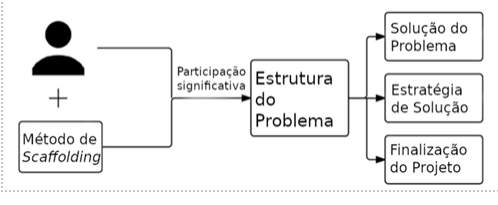
\includegraphics[width=0.8\textwidth]{fig/scaffoldinInstitucional.png}
\label{fig:scaffoldingInstitucional}
\caption*{Fonte: Adaptado de \citeonline{Belland2017}.}
\end{center}
\end{figure}

Entretanto, devemos tomar cuidado ao classificar uma “ajuda” como parte do processo de \textit{Scaffolding}. Isso ocorre, pois, muitas vezes durante o processo de análise dessa ajuda, passamos a chamar de \textit{Scaffolding} toda e qualquer ajuda que auxilie o aluno na resolução do problema. Tal informação é inexata, uma vez que dizer o quê ou como deve ser feito determinada tarefa não pode ser considerada como \textit{Scaffolding}(\cite{Belland2017}, uma vez que esse tipo de abordagem não faz uso nem se constrói a partir do conhecimento prévios do aluno. 

Para que possamos classificar uma ajuda como parte do método de \textit{Scaffolding} é extremamente necessário que a ajuda fornecida faça uso dos conhecimentos prévios do aluno, para que ele possa construir seus novos conhecimentos em cima de seus conhecimentos prévios. Inclusive, o termo \textit{Scaffolding} do inglês significa andaime, uma alusão direta aos andaimes utilizados na construção civil. 

Assim como os andaimes da construção servem de ancoragem para a construção de uma estrutura mais rígida e definitiva, o andaime na educação que estamos chamando de \textit{Scaffolding} serve como ancoragem para a formação de um conhecimento mais sólido sobre o problema a ser trabalhado. E esses “andaimes” podem ser fornecidos por professores, colegas ou, até mesmo, por ferramentas computacionais. 

O método de \textit{Scaffolding} também é composto por três principais elementos: Avaliação Dinâmica, Fornecer a Quantidade Certa de Suporte e Intersubjetividade. Esses três elementos serão descritos a seguir. 

\section{AVALIAÇÃO DINÂMICA}

A avaliação dinâmica está intrinsecamente conectada com a customização do método de \textit{Scaffolding} \cite{Belland2017,wood1976}. A Figura 2 exemplifica a relação entre a avaliação dinâmica e o \textit{Scaffolding}.

\begin{figure}[htp]
\begin{center}
\caption{O papel da Avaliação Dinâmica na Customização do \textit{Scaffolding}.}
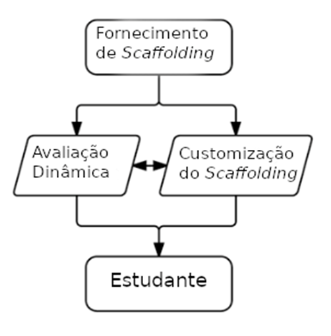
\includegraphics[width=0.7\textwidth]{fig/avaliacaodinamica.png}
\label{fig:avadinamica}
\caption*{Fonte: Adaptado de \citeonline{Belland2017}.}
\end{center}
\end{figure}

A avaliação Dinâmica pode envolver uma série de instruções, onde cada instrução pode ter diferentes níveis de suporte. Então o professor pode determinar, para o atual nível de habilidade do aluno, qual destes suportes é necessário para permitir o desempenho adequado do aluno na tarefa. 

Ao associar a Avaliação Dinâmica com o \textit{Scaffolding}, \citeonline{Belland2017} ressalta que: 

\begin{quoting}[leftmargin=4cm, rightmargin=0cm]
\noindent Avaliação dinâmica pode também ser usada para ajustar o \textit{Scaffolding} que já está sendo fornecido. Neste caso, os professores podem determinar até que ponto a habilidade do aluno está melhorando, de modo a levar ao sucesso sem o uso, ou com menor uso, de \textit{Scaffolding}. E tais ajustes podem ser feitos em tempo real. 
\end{quoting}

\section{FORNECER A QUANTIDADE CERTA DE SUPORTE}

O fornecimento da quantidade certa de suporte se refere a fornecer a suporte ao Scaffolding de acordo com a indicação da avaliação dinâmica \cite{wood1976,Belland2017}. Isso pode ser feito tanto pelo fornecimento de suporte em tempo real \cite{Jadallah2011,vanPol2012,Belland2017}, ou fornecendo a combinação certa de elementos prévios de Scaffolding \cite{Koedinger2006,Belland2017}. Além disso, de acordo com \citeonline[p.18]{Belland2017} e \citeonline[p.17]{wood2003}, providenciar a quantidade correta de suporte depende dos ajustes em uma ou mais das seguintes formas: ajuste das estratégias de suporte que estão sendo utilizadas, as sub-habilidades cujo foco esteja próximo, e o tempo necessário oferecido para o suporte. 

\citeonline{Koedinger2006,Koedinger2007,Belland2017} ressaltam, sobre o ajuste de \textit{Scaffolding}: 

\begin{quoting}[leftmargin=4cm, rightmargin=0cm]
\noindent O ajuste de \textit{Scaffolding} também pode assumir a forma de adicionar diferentes tipos de suporte ou aprimorar o suporte que já estava presente. Isso com base na avaliação dinâmica que indica que os alunos não estão progredindo rápido o suficiente para levar à solução independente da solução de problemas. 
\end{quoting}

Por fim, podemos dizer que, ao fornecer a quantidade certa se suporte ao \textit{Scaffolding}, temos como meta que o aluno não apenas ganhe as habilidades necessárias para realizar a tarefa de forma independente, mas que também assume responsabilidade pela execução da própria tarefa \cite{wood1976,Belland2014, Belland2017}. Em outras palavras, estamos dizendo que queremos que o aluno não apenas desenvolva suas capacidades, mas também tenha mais vontade de resolver tarefas complexas de forma independente \cite{Belland2013, Belland2017}. 

\section{INTERSUBJETIVIDADE}

A intersubjetividade é crucial para a definição de \textit{Scaffolding} e para a ideia de transferir responsabilidades para o aluno. Segundo a intersubjetividade, os alunos precisam ser capazes de reconhecer uma solução apropriada para problemas semelhantes, antes de serem capazes de executar a mesma tarefa de forma independente \cite{wood1976,Mortimer2009,Mahardale2014,Belland2017}. De acordo com \citeonline[p.16]{Belland2017}, sem a intersubjetividade os alunos são considerados incapazes de se engajar no desempenho independente da habilidade alvo apresentado na Figura \ref{fig:intersubjetividade}. 

\begin{figure}[htp]
\begin{center}
\caption{Exposição da Intersubjetividade e Engajamento no \textit{Scaffolding}.}
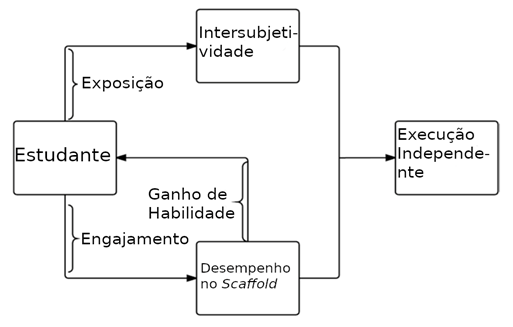
\includegraphics[width=0.7\textwidth]{fig/intersubjetividade.png}
\label{fig:intersubjetividade}
\caption*{Fonte: Adaptado de \citeonline{Belland2017}.}
\end{center}
\end{figure}

De acordo com \citeonline[p.22]{Belland2017} e \citeonline{wertsch2005}, a intersubjetividade pode ser alcançada sem o conhecimento de como executar a habilidade que o \textit{Scaffolding} se destina a desenvolver. Para \citeonline[p.21]{Belland2017} e \citeonline{Rogoff1997}, é importante que notemos que não é necessário existir um mesmo entendimento entre aluno e professor.  Isso ocorre, pois, parceiros em uma mesma atividade possuem perspectiva diferentes, o que pode moldar o entendimento da tarefa. Além disso, para \citeonline[p.22]{Belland2017} e \cite{wertsch1985zone}, se uma criança e um adulto tivessem uma compreensão idêntica de qual seria a solução mais apropriada para um problema semelhante ao que está sendo abordado, então pode ser criança não precise de \textit{Scaffolding}. 

\section{FORMAS DE SCAFFOLDING}

Podemos classificar, segundo \citeonline[p.22]{Belland2017}, três formas de trabalhar com o método de Scaffolding. Essas formas podem ser separadas em: \textit{Scaffolding} Um a Um (SUU), \textit{Scaffolding} por Pares (SPP) e \textit{Scaffolding} Baseado em Computadores (SBC). 

A Tabela \ref{tab:tipsScaf} exemplifica a comparação entre as três formas de \textit{Scaffolding}. As três formas de \textit{Scaffolding} serão descritas na sequência do trabalho. 

\begin{comment}
\setlength{\tabcolsep}{1.505625pt}
\renewcommand{\arraystretch}{1.2}
\begin{table}[ht]
\captionof{table}{Visão Geral dos tipos de \textit{Scaffolding}.}
\label{tab:tipsScaf}
\begin{tabular}{|l|l|l|l|}
\hline
\multicolumn{1}{|p{82.80937pt}}{} & \multicolumn{1}{|p{114.4275pt}}{\centering {\bfseries \textit{Scaffolding} Um a Um }} & \multicolumn{1}{|p{112.921875pt}}{\centering {\bfseries \textit{Scaffolding} Baseado em Computador }} & \multicolumn{1}{|p{113.67469pt}|}{\centering {\bfseries \textit{Scaffolding} por Pares }}\\ \hline

\multicolumn{1}{|p{82.80937pt}}{\centering {\bfseries O que \'e? }} & \multicolumn{1}{|p{114.4275pt}}{\centering Professor trabalhando individualmente com um estudante } & \multicolumn{1}{|p{112.921875pt}}{\centering Fun\c{c}\~ao do \textit{Scaffolding} cumprida por uma ferramenta computacional que pode ser incorporada no curr\'{\i}culo ou uma ferramenta que os estudantes usem quando se engajam em um problema fora do sistema } & \multicolumn{1}{|p{113.67469pt}|}{\centering \textit{Scaffolding} promovido por pares com habilidades superiores ou de mesmo n\'{\i}vel }\\ 
\hline 
\multicolumn{1}{|p{82.80937pt}}{\centering {\bfseries Entre as formas de \textit{Scaffolding}, quais suas vantagens relativas? }} & \multicolumn{1}{|p{114.4275pt}}{\centering Leva \`a influ\^encia mais forte nos resultados de aprendizagem \\ 
\strut\ \\ 
\'E o melhor para a customiza\c{c}\~ao din\^amica } & \multicolumn{1}{|p{112.921875pt}}{\centering \'E o mais utiliz\'avel \\ 
\strut\ \\ 
Tem paci\^encia infinita } & \multicolumn{1}{|p{113.67469pt}|}{\centering \'E a forma mais utiliz\'avel de \textit{Scaffolding} que envolve intera\c{c}\~oes individuais }\\ 
\hline 
\multicolumn{1}{|p{82.80937pt}}{\centering {\bfseries Entre as formas de \textit{Scaffolding}, quais suas desvantagens relativas? }} & \multicolumn{1}{|p{114.4275pt}}{\centering Menos utiliz\'avel } & \multicolumn{1}{|p{112.921875pt}}{\centering Menos din\^amico } & \multicolumn{1}{|p{113.67469pt}|}{\centering Provedor de Scaffolding n\~ao \'e, necessariamente, mais h\'abil }\\ 
\hline 
\end{tabular}
\caption*{Fonte: Construção do Autor.}
\end{table}
\end{comment}


\begin{table}[ht]
\caption{Visão Geral dos tipos de \textit{Scaffolding}.}
\label{tab:tipsScaf}
\begin{tabular}{p{82.80937pt}|p{114.4275pt}|p{112.921875pt}|p{113.67469pt}}
\hline
\textbf{} & \textbf{\textit{Scaffolding} Um a Um} & \textbf{\textit{Scaffolding} Baseado em Computador} & \textbf{\textit{Scaffolding} por Pares}\\ 
\hline
\textbf{O que é?} & Professor trabalhando individualmente com um estudante & Função do \textit{Scaffolding} cumprida por uma ferramenta computacional que pode ser incorporada no currículo ou uma ferramenta que os estudantes usem quando se engajam em um problema fora do sistema & \textit{Scaffolding} promovido por pares com habilidades superiores ou de mesmo nível\\ 
\hline
\textbf{Entre as formas de \textit{Scaffolding}, quais suas vantagens relativas?} & Leva à influência mais forte nos resultados de aprendizagem & É o mais utilizável & Tem paciência infinita\\ 
\hline
\textbf{Entre as formas de \textit{Scaffolding}, quais suas desvantagens relativas?} & Menos utilizável & Menos dinâmico & Provedor de Scaffolding não é, necessariamente, mais habil\\ 
\hline
\end{tabular}
\caption*{Fonte: Construção do Autor.}
\end{table}

\subsection{\textit{Scaffolding} Um a Um}

\citeonline[p.21]{Belland2017} define o SUU como sendo um professor trabalhando individualmente com um estudante para avaliar dinamicamente o nível atual do estudante, provendo a quantidade correta de suporte para que o estudante para que ele ganhe a habilidade na tarefa em questão. Além de personalizar o suporte conforme necessário até que o \textit{Scaffolding} possa ser completamente retirado e o estudante possa executar a tarefa de forma independente \cite{Chi1996,Graesser1997,Lepper1997,vanPol2010,Belland2014}.
 
A utilização do Scaffolding Um a Um é útil ao pensarmos nas intenções do método de Scaffolding, seja na utilização pelo professor, nos meios utilizados, e nas estratégias específicas utilizadas \cite{vanPol2010,Belland2012,Belland2017}. As intenções do SUU incluem o recrutamento, estruturação das tarefas, manutenção da direção, redução dos graus de liberdade e controle de frustração \cite{vanPol2010,Belland2017}.

De acordo com \citeonline[p.27]{Belland2017}, as formas de utilização do SUU incluem modelar, questionar, explicar, dar dicas e providenciar um \textit{feedback} \cite{vanPol2010}. \citeonline[p.22]{Belland2017} e \citeonline{Lin2014} dizem que: 

\begin{quoting}[leftmargin=4cm, rightmargin=0cm]
\noindent Para promover a consideração das relações entre as diferentes individualidades envolvidas em um problema, o professor pode levar os alunos a considerar tais relações e ilustrar como fazê-lo. 
\end{quoting}

\citeonline[p.23]{Belland2017} conclui dizendo que, devido a forma altamente contagiante de sua estrutura, o SUU é geralmente considerado como sendo a forma ideal de \textit{Scaffolding} \cite{Chi1996,Graesser1997,Belland2015}. Entre todas as formas de \textit{Scaffolding} , \citeonline[p.24]{Belland2014} diz que SUU tende a levar aos melhores resultados, conforme indica o trabalho de \citeonline[p.1]{vanLehn2011}.  
\subsection{\textit{Scaffolding} Por Pares }

\textit{Scaffolding}por pares se refere ao fornecimento de suporte por pares de mesma idade ou conhecimento similar e exalta a força do número de pares em salas de aula \cite{Pata2006,Davin2013,Sabet2013,Belland2017}. Porém, o SPP pode também envolver crianças mais velhas que dão suporte a crianças mais jovens, com o uso de seus conhecimentos sobre a tarefa em questão. 

\citeonline[p.21]{Belland2014} e  \citeonline[p.25]{Belland2017}, sugere que o SPP necessita o fornecimento de uma estrutura que oriente o desenvolvimento do suporte provido por \textit{Scaffolding}. Onde essa estrutura pode guiar o fornecedor desse suporte com a forma e o momento de uso de estratégias de \textit{Scaffolding}.

Para finalizar, \citeonline[p.21]{Belland2014} e  \citeonline[p.25]{Belland2017}, conclui que: 

\begin{quoting}[leftmargin=4cm, rightmargin=0cm]
\noindent É improvável que \textit{Scaffolding} por pares seja suficiente como forma única de suporte por \textit{Scaffolding}, uma vez que os pares com capacidades semelhantes não têm conteúdo ou a experiência pedagógica necessária para se envolverem na avaliação dinâmica e na personalização que é característica do \textit{Scaffolding} por Pares. 
\end{quoting}
\subsection{\textit{Scaffolding} Baseado em Computador}

De acordo com \citeonline[p.1]{Belland2017}, \textit{Scaffolding} baseado em computador auxilia os estudantes a se engajarem e adquirirem habilidades em tarefas que estão além de suas habilidades não assistidas \cite{Hannafin1999,Quintana2004,Belland2014}. Especificamente, o SBC ajuda os estudantes na geração de soluções para problemas complexos e mal estruturados, e é fornecido inteiramente por uma ferramenta baseada em computador \cite{Belland2017}.

Isso significa que uma ferramenta computacional é capaz de ampliar a capacidade dos alunos de forma que eles se tornam capazes de realizar tarefas que estão em um nível mais alto que suas capacidades atuais não assistidas. \citeonline[p.21]{Belland2017} afirma que “\textit{Scaffolding} baseado em computador tem tido um tamanho de efeito muito substancial em pesquisas anteriores, em comparação com intervenções semelhantes, e isso merece mais pesquisas metodologia”. 
\chapter{Aplicações}\label{ch:apl}

Neste Capítulo serão descritos os modelos das atividades aplicadas. As atividades foram divididas em dois tipos principais: Oficinas de Resolução de Problemas (ORP) e Atividades de Sala de Aula (ASA). No Capítulo \ref{ch:resanddisc} serão detalhadas algumas particularidades de cada aplicação, bem como os resultados e observações obtidos, dando continuidade às informações contidas no presente capítulo.

Na Seção \ref{sec:orp} são descritas as origens das ORP, a partir do contexto social em que estávamos inseridos, e suas modificações. Foram realizadas três oficinas ao todo, sendo que houve a necessidade de um \textit{redesign} para sua continuidade.

Na Seção \ref{sec:asa} estão descritas as ASA, as quais tiveram, assim como as ORP, três aplicações. As Atividades de Sala de Aula surgiram de um \textit{redesign} a partir de necessidades surgidas dos desdobramentos encontrados nas ORP.

\section{Oficinas de Resolução de Problemas} \label{sec:orp}

A Figura \ref{fig:ativEvo} mostra a evolução das atividades aplicadas ao longo deste trabalho. De forma sucinta, a ORP 1, representada em Azul passa por um processo de \textit{redesign} (em Verde) gerando um novo padrão de ORP. 

Esse novo padrão é representado pelas ORP 2 e ORP 3 (em Verde). Os resultados obtidos por estas ORP favoreceram a formação de um novo \textit{redesign}, representado em Laranja. Esse \textit{redesign} aplicado às duas ORP da origem às ASA.

\begin{figure}[htp]
\begin{center}
\caption{Evolução das atividades}
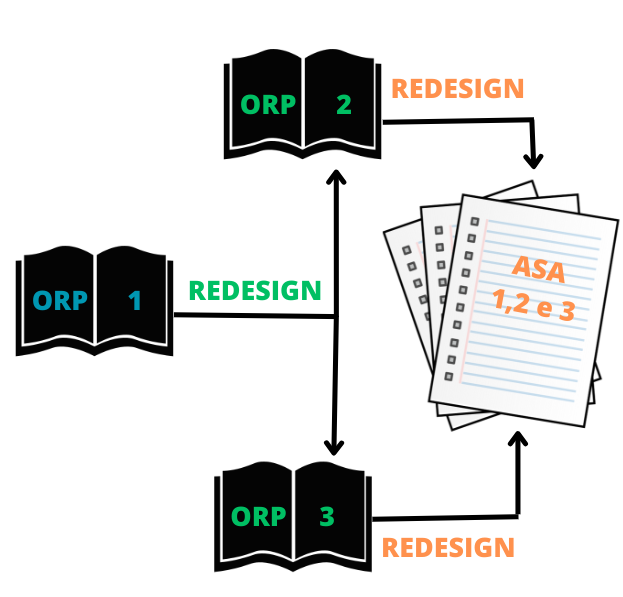
\includegraphics[width=0.9\textwidth]{fig/resumoatovodades.png}
\label{fig:ativEvo}
\caption*{Fonte: Criação do Autor.}
\end{center}
\end{figure}

Dessa forma, aplicamos os conceitos do EDR (a partir do \textit{redesign}), dentro dos modelos de aplicação da RP. E esses modelos estão baseados na metodologia de \textit{Scaffolding}. Assim, conseguimos perceber a conexão do tripé \textit{Scaffolding}, RP e EDR.

O processo de desenvolvimento desta dissertação iniciou no final do ano de 2019, com a redação do pré-projeto de pesquisa feito para o ingresso no programa de pós-graduação (que ocorreu no primeiro semestre de 2020). A proposta inicial era de fazer uma aplicação computacional (SBC). Nessa proposta o aluno receberia uma questão por vez, tendo a opção de solicitar uma dica, caso necessitasse. O próprio software forneceria opções de dicas para o aluno que escolheria uma opção mais próxima de sua necessidade.

Para cada questão seria atribuída uma pontuação. Essa pontuação teria seu valor máximo reduzido, à medida que o aluno fosse fazendo uso das dicas disponíveis. Neste Capítulo traremos uma análise sobre as observações obtidas ao longo das três oficinas de resolução de problemas. Para isso, escrevemos três Seções, uma para cada oficina. Relembrando, intitulamos como Primeira Oficina àquela aplicada a uma turma de Física Básica logo no início do período da pandemia.  

A Segunda Oficina foi aplicada também a uma turma de Física Básica, porém já havendo retornado as aulas presenciais. Por fim, a Terceira Oficina foi aplicada, ao mesmo tempo da Segunda Oficina, mas em uma turma de Física Avançada. 

Como já foi explicado, na Seção anterior, o funcionamento individual de cada oficina, aqui trataremos das observações e impressões de cada uma. Além disso, traremos algumas informações adicionais que possam ser de interesse. 

A função do \textit{Scaffolding} é manter o aluno trabalhando, sem que ele desista da questão. De forma com que o aluno consiga fazer o seu melhor durante o processo de resolução, mesmo que para isso acabe obtendo uma pontuação mais baixa.

Porém, em 17 de março de 2020, foi postado no \citeonline{portaria343}, sob a portaria número 343, a autorização para as aulas à distância nas Universidades Federais. Isso ocorreu por virtude do aumento de contaminações por causa da pandemia de Coronavírus em todo o território nacional. Dessa forma, a Universidade Federal de Santa Maria optou por fazer uso de aulas remotas, a fim de tentar conter os casos de contaminação dos alunos, professores e servidores da instituição, sem precisar cancelar o semestre letivo. 

Dessa forma, com as aulas da pós-graduação em regime remoto, e com incerteza sobre a volta à normalidade, foi necessário reestruturar o projeto para caber numa nova realidade. Com a proximidade do segundo semestre letivo e a falta de perspectiva de volta às aulas presenciais, estruturamos o que chamamos de Oficinas de Resolução de Problemas em seu primeiro \textit{design}.

\subsection{Primeira Oficina} \label{subsec: primeiraof}

Com os problemas advindos do isolamento social e do regime de aulas remotas, surgiu uma necessidade de adaptar o modelo tradicional de aulas e avaliações para o sistema \textit{online}. Aproveitamos a situação, simplificamos e reestruturamos o modelo originalmente pensado para trabalhar a Resolução de Problemas através do \textit{Scaffolding} no contexto remoto em turmas de Ensino Superior. Chamaremos esta aplicação de primeira Oficina de Resolução de Problemas (ORP1).

Após o professor trabalhar o conteúdo da disciplina em aula, seria aplicado um problema sobre o conteúdo para que os alunos resolvessem. Como estavam em regime remoto de aulas, esse processo resolutivo deveria ser feita durante o horário de aula, com a câmera ligada. Após o término da questão, os alunos deveriam tirar uma foto de sua resolução e entregar, eletronicamente, para que o tutor da disciplina corrigisse.

Ao corrigir as questões dos alunos, o tutor fornecia uma nota e um \textit{feedback} do processo de resolução. Esse \textit{feedback} fornecia informações como: erros matemáticos, dificuldade de interpretação, falta de etapas, repostas incompletas, entre outras informações que o tutor considerasse importante para que a questão fosse considerada correta.

Dessa forma o \textit{feedback} tem a mesma função das dicas, que é essencial para o processo de \textit{Scaffolding}. Os alunos que tivessem uma nota inferior a um valor estipulado pelo professor poderiam fazer uma Atividade Substitutiva. Essa atividade seria fornecida pelo tutor e teria uma estrutura de resolução similar à Atividade Síncrona.

Ou seja, os alunos poderiam utilizar as informações contidas no \textit{feedback} para fazer uma nova questão e, assim, melhorar sua nota. Como contrapartida, essa Substitutiva teria uma pontuação máxima inferior à pontuação máxima da Atividade Síncrona.

Por questões de tempo, quem optasse por resolver a Atividade Substitutiva teria um prazo de $24$ $h$ para a conclusão e entrega da mesma. Essa entrega se daria, novamente, por meio eletrônico. A questão aplicada, nessa situação, seria a mesma para todos os alunos, e todos teriam acesso à questão antes de escolher resolvê-la. Ou seja, os alunos poderiam analisar se conseguiriam resolver a questão antes mesmo de optar em resolvê-la.

Ao desenvolvermos desta maneira a ORP1, pudemos verificar o \textit{Scaffolding} dentro do processo de RP. Neste caso, o \textit{feedback} (dicas) é aplicado a todos os alunos, independentemente de solicitarem ou não. A aplicabilidade das informações do \textit{feedback} também varia, pois não controlamos se os alunos vão ler as informações após terem a devolutiva da Atividade Síncrona. Além disso, fazer a Atividade Substitutiva é opcional e depende inteiramente do aluno.

As ferramentas que dispomos para analisar os resultados da ORP1 são: as notas dos alunos, as folhas de resolução, as anotações do tutor acerca das resoluções e um questionário aplicado ao término do semestre. Analisando as folhas de resolução, devemos ser capazes de responder aos questionamentos dos objetivos específicos \ref{item:a}, \ref{item:b}, \ref{item:c} e \ref{item:e}.

O questionário pode servir para responder aos objetivos específicos \ref{item:b}, \ref{item:d} e \ref{item:e}. As notas do alunos podem ajudar a compreender os objetivos específicos \ref{item:c} e \ref{item:e}. As anotações do tutor podem ser úteis na resposta dos questionamentos \ref{item:b}, \ref{item:d} e \ref{item:e}.

Apesar disso, se faz necessária uma análise conjunta de todos os objetos utilizados para responder a estes questionamentos. E, partindo de uma reflexão sobre esses resultados, devemos ser capazes de responder o questionamento do objetivo principal deste trabalho.

A ORP1 funcionou muito bem como um teste. Seus resultados não foram expressivos, como mostraremos na Seção \ref{sec:orp1}. Surgiu uma necessidade de reaplicação e, para isso, foi elaborado um \textit{redesign} que culminou na Segunda e Terceira ORP, que chamaremos de ORP2 e ORP3, respectivamente.

\subsection{Segunda e Terceira Oficinas} \label{sec:orp2e3}

Após a conclusão da ORP1, passamos um semestre pesquisando e estudando mais a fundo os conceitos de \textit{Scaffolding} e de RP. Os resultados obtidos até então não forneciam uma base segura de informações sobre a eficácia da metodologia, nos trazendo a necessidade de testar o \textit{Scaffolding} novamente.

Nesse período, a vacinação contra o Coronavírus já estava avançada no país e as aulas presenciais estavam na iminência de retornar. Por isso, durante o processo de \textit{redesign}, precisamos levar em consideração a volta à presencialidade como critério a ser adaptado.

Continuaríamos trabalhando com turmas de Ensino Superior. Porém, após revisitarmos os dados obtidos na ORP1, surgiu o interesse em analisar as diferenças nos processos de RP entre estudantes Principiantes e Especialistas. Assim, pensamos em estruturar essa versão da ORP de maneira que pudesse ser aplicada tanto em turmas de Principiantes quanto de Especialistas em Física.

Por isso que, nesta seção, tratamos da ORP2 e ORP3 ao mesmo tempo. Afinal, elas constituem, em si, o mesmo modelo de atividade. O que as difere, como será visto nas Seções \ref{sec:2orp} e \ref{sec:3orp}, são as turmas para as quais elas são aplicadas.

Agora, nosso novo \textit{design} passará a trabalhar com um processo de SUU. Os alunos continuariam tendo aula com o professor regente onde, após a conclusão de algum conteúdo (definido pelo próprio professor), seria aplicada uma lista de problemas.

Esta lista deveria conter, obrigatoriamente, questões do último conteúdo finalizado em aula. Para auxiliar os estudantes, um tutor ficaria à disposição para ajudá-los em suas dúvidas. Os alunos seriam incentivados a pedir ajuda caso não conseguissem prosseguir no processo de resolução das questões.

Assim, o tutor orienta individualmente (SUU) o estudante, e daria as dicas necessárias para que o estudante conseguisse prosseguir na resolução. Para que o professor regente pudesse dar continuidade à ementa da disciplina, era necessário que os alunos conseguissem resolver as listas de problemas.

Nas aplicações da ORP2 e ORP3 eram os alunos que ditavam o ritmo da aula. O processo de \textit{Scaffolding} ocorreria nas intervenções do tutor mediante as dúvidas dos alunos. Já os estudantes eram incentivados a resolver as listas da melhor forma possível e no menor tempo possível, para que o professor regente pudesse dar continuidade ao conteúdo.

Neste processo, a avaliação dos alunos - por parte da disciplina - estava associada ao progresso dos alunos no conteúdo de sala de aula. Quanto mais conteúdos da ementa o professor conseguisse trabalhar em sala, melhor seria o desempenho dos alunos na disciplina. Ou seja, os alunos eram incentivados a progredir na resolução das listas para que pudessem ser aprovados.

Entretanto, o progresso na resolução das listas não era fator único e exclusivo para o professor avaliar a aprovação ou reprovação dos acadêmicos. O desempenho dos mesmos durante as aulas de resolução das listas seria avaliado. Esta análise caberia ao tutor, que além de auxiliar no processo de resolução deveria observar e analisar o desenvolvimento dos acadêmicos ao longo do período letivo.

Os objetos que dispomos na ORP2 e ORP3 para responder aos questionamentos dos objetivos são as folhas de resolução dos alunos e as anotações do tutor durante o processo de aplicação. Como existe uma relação muito próxima entre o tutor e o tutorado no processo do SUU, a análise dos cinco objetivos secundários e do objetivo principal serão feitas utilizando em conjunto as anotações e as folhas de resolução.

Podemos ressaltar, ainda, que neste estágio de desenvolvimento do trabalho não dispúnhamos de uma classificação própria para os tipos de dicas. Esse tipo de classificação foi desenvolvido para as Atividades de Sala de Aula, que serão descritos na Seção \ref{sec:asa}. E este processo foi desenvolvido a partir de um \textit{redesign} mais robusto do modelo de aplicação, onde conseguiríamos aplicar a mesma metodologia em mais de uma turma com graus de instrução semelhantes.

\section{Atividades de Sala de Aula} \label{sec:asa}
%% Ver uma introdução
Discutiremos no Capítulo \ref{ch:resanddisc} os motivos de sermos levados a um novo processo de \textit{redesign} após a aplicação da ORP2 e ORP3. Porém, precisamos antecipar que um desses motivos, e talvez o principal deles, fosse a necessidade de estudarmos turmas com mais alunos.

Com as diferenças que começavam a surgir neste novo \textit{design} com relação às ORP, acabamos por renomear este novo conjunto de atividades para Atividades de Sala de Aula. As ASA, então, forma um conjunto de atividades didáticas pensadas e formuladas para avaliar a metodologia de \textit{Scaffolding} na competência de RP, agora, para estudantes do Ensino Médio.

Outro fator a ser repensado foi o modelo de lista de questões. Em turmas menores, fazia sentido apresentar uma lista de questões para que eles resolvessem. Até porque seria relativamente fácil de acompanhar, auxiliar e dar as dicas necessárias. Além disso, quando trabalhamos com o modelo de listas, os estudantes tinham, em teoria, um bom embasamento matemático, por se tratar de cursos universitários, e conseguiriam progredir com mais facilidade. 

Quando pensamos na mudança do nosso público-alvo, pensamos também nas dificuldades de leitura e interpretação dos mesmos, além de lacunas nos conhecimentos matemáticos. Essa estruturação foi possível pois, durante o processo de \textit{redesign}, já tínhamos conhecimento prévio sobre as turmas. Esse foi um grande diferencial das outras aplicações, onde não tínhamos conhecimento das turmas até o início do período letivo.

Pensando nestes fatores, este novo design da atividade conta com apenas uma questão. Esta questão deveria ser composta por um problema similar ao que eles trabalharam ou viram em sala de aula. Para que estas questões fossem, realmente, problemas, ao invés de exercícios, adicionamos uma ou duas etapas a mais, de forma que o nível de exigência aumentasse. Na Tabela \ref{ref:questoes} temos um exemplo de questão trabalhada em sala de aula e sua adaptação para uma possível ASA.  

\begin{comment}
\begin{table}[ht]
\caption{Diferença entre questão do livro e adaptada para ASA.}
\label{ref:questoes}
\centering
\begin{tabular}{|p{0.45\linewidth}|p{0.45\linewidth}|}
\hline
\textbf{Atividades do Livro} & \textbf{Atividades de Sala de Aula} \\
\hline
(UPF-RS) Qual a quantidade de calor que devemos fornecer a 200g de gelo a -20°C para transformar em água a 50°C?
\newline Considere:
\newline $c_{gelo} = 0,5 \, \text{cal/g}^{\circ}C$
\newline $c_{agua} = 1 \, \text{cal/g}^{\circ}C$
\newline $L_{fusao} = 80 \, \text{cal/g}$
\begin{itemize}
    \item[a)] 28 kcal
    \item[b)] 26 kcal
    \item[c)] 16 kcal
    \item[d)] 12 kcal
    \item[e)] 18 kcal
\end{itemize} 
& 
(UPF-RS/Adaptada) Qual a quantidade de calor que devemos fornecer a 500g de gelo a -5°C para transformar em vapor de água a 120°C? 
\newline Considere:
\newline $c_{gelo} = 0,5 \, \text{cal/g}^{\circ}C$
\newline $c_{agua} = 1 \, \text{cal/g}^{\circ}C$
\newline $c_{vapor} = 4,48 \, \text{cal/g}^{\circ}C$
\newline $L_{fusao} = 80 \, \text{cal/g}$
\newline $L_{vaporizacao} = 540 \, \text{cal/g}$
\\
\hline
\end{tabular}
\caption*{Fonte: Construção do Autor.}
\end{table}
\end{comment}

\begin{table}[ht]
\caption{Diferença entre questão do livro e adaptada para ASA.}
\label{ref:questoes}
\centering
\begin{tabular}{p{0.45\linewidth}|p{0.45\linewidth}}
\hline
\textbf{Atividades do Livro} & \textbf{Atividades de Sala de Aula} \\
\hline
(UPF-RS) Qual a quantidade de calor que devemos fornecer a 200g de gelo a -20°C para transformar em água a 50°C?
\newline Considere:
\newline $c_{gelo} = 0,5 \, \text{cal/g}^{\circ}C$
\newline $c_{agua} = 1 \, \text{cal/g}^{\circ}C$
\newline $L_{fusao} = 80 \, \text{cal/g}$
\begin{itemize}
    \item[a)] 28 kcal
    \item[b)] 26 kcal
    \item[c)] 16 kcal
    \item[d)] 12 kcal
    \item[e)] 18 kcal
\end{itemize} 
& 
(UPF-RS/Adaptada) Qual a quantidade de calor que devemos fornecer a 500g de gelo a -5°C para transformar em vapor de água a 120°C? 
\newline Considere:
\newline $c_{gelo} = 0,5 \, \text{cal/g}^{\circ}C$
\newline $c_{agua} = 1 \, \text{cal/g}^{\circ}C$
\newline $c_{vapor} = 4,48 \, \text{cal/g}^{\circ}C$
\newline $L_{fusao} = 80 \, \text{cal/g}$
\newline $L_{vaporizacao} = 540 \, \text{cal/g}$
\\
\hline
\end{tabular}
\caption*{Fonte: Construção do Autor.}
\end{table}

Neste novo \textit{design}, o fornecimento de dicas depende exclusivamente do aluno. É função do estudante chamar o professor e solicitar uma dica quando não conseguir prosseguir com a resolução da questão. Cada estudante pode pedir até cinco dicas, onde o professor avalia a pergunta feita pelo aluno e fornece a melhor resposta para ele. 

No Apêndice \ref{ch:modeloASA} temos a folha modelo de aplicação das ASA. Nela podemos ver que as regras toras especificadas para os alunos, na parte superior. Além disso, a parte inferior da folha conta com um espaço para que sejam inseridas as dicas que o professor achar pertinente fornecer aos estudantes mediante solicitação. 

Podemos perceber, pela forma como as dicas são fornecidas aos alunos, que continuamos com um processo de SUU. Porém, neste caso, essas dicas são mais pontuais e, em grande parte, preparadas previamente. De forma que o professor, antes de propor a tarefa, antecipa as possíveis dificuldades dos alunos para que ele possa auxiliá-los de forma mais eficaz.

As ASA são, então, constituídas por apenas um problema dissertativo, que pode contar com mais de uma pergunta para ser respondida. Os alunos teriam o tempo de um período de aula (45 minutos) para a realização da atividade. Neste período de tempo está incluso a organização da turma para a realização da atividade. Ou seja, quanto mais tempo os alunos demorassem para se organizar, menos tempo para a resolução eles teriam. 

Quando surgisse alguma dificuldade durante o processo de resolução, o estudante poderia fazer uma pergunta ao professor. O professor, então, analisaria o desenvolvimento do aluno e forneceria uma dica de forma a orientar o estudante nesta etapa de superação da dificuldade. Em contrapartida, para cada dica dada o valor máximo da questão era reduzido em um ponto. 

Todas as atividades começam com um valor máximo de dez pontos e podem chegar ao menor valor máximo possível, de cinco pontos, caso o aluno tenha solicitado cinco dicas. Todos os alunos eram atendidos conforme a demanda aparecia, e os tipos de dicas e dificuldades eram variados para os alunos. 

Para que as dicas fossem fornecidas era necessário que o aluno fizesse uma pergunta objetiva sobre o conteúdo, ou sobre a questão em si. Para casos em que os alunos simplesmente pedissem uma dica, sem explicitar o que já sabem, ou sem demonstrar o que haviam entendido ou feito, era necessário um tipo diferente de ajuda. 

Pensando nestas possibilidades, conseguimos agrupar as dúvidas dos alunos em dois tipos: as dúvidas Qualificadas e as dúvidas Desqualificadas\footnote{As dicas de perguntas Desqualificadas podem ser também interpretadas como dicas de perguntas Não Qualificadas. Não queremos dar juízo de valor às dicas, apenas tipificar os tipos de perguntas que elas respondem.}. Nas dúvidas Qualificadas, o aluno sabe exatamente o que precisa para prosseguir com a questão. Ele consegue traduzir em palavras o que entendeu do problema e formular uma pergunta cuja resposta o ajude a superar este obstáculo. 

Quando falamos das dúvidas Desqualificadas, não queremos dizer que elas sejam sem importância. Mas que elas servem de fator de alerta para algumas possibilidades: o aluno não compreende a matéria, ou tem dificuldade de interpretação, ou não estudou, ou não considera o assunto relevante, ou uma série de outras possibilidades que talvez nem passem pela nossa cabeça. Nestes casos, o processo de auxílio é muito mais do que simplesmente fornecer uma dica. Ele implica em entender o que está acontecendo com o aluno que chegou nesse estágio. 

Para conseguirmos trabalhar com os casos que apareceriam de dúvidas Desqualificadas, optamos por seguir o modelo de \citeonline{Pozo2009} para a RP. Já para as dúvidas Qualificadas, tentamos separar as dicas em três categorias: dicas de localização, dicas de conteúdo e dicas de matemática. 

As dicas de localização são as responsáveis por auxiliar o aluno que tem dificuldade em entender de que parte do conteúdo faz parte a questão. Como o projeto foi aplicado em sala de aula, foi necessário que se seguisse a sequência do material da escola. No caso, alguns capítulos do livro dos estudantes continham mais de um conteúdo, logo as dicas de localização se fariam necessárias. 

As dicas de conteúdo são referentes aos tópicos trabalhados em sala de aula. São dicas como as equações, propriamente ditas, ou algum detalhe da parte teórica que possa ter pego o aluno desprevenido. 

Por fim, as dicas do de matemática surgem quando os alunos erram ou não consegue desenvolver alguma operação própria da matemática. Este tipo de dica acaba sendo muito pessoal de cada aluno pois leva em consideração as dificuldades preexistentes em seus conhecimentos. Quando pensamos no \textit{redesign} da atividade, levamos em consideração essa possibilidade de dificuldade por parte dos alunos.   

Na criação deste novo \textit{design} foi necessário compreender como estas atividades se conectam com os objetivos da pesquisa. Quanto ao objetivo principal – verificar se a metodologia de \textit{Scaffolding} contribui para o desenvolvimento da competência da resolução de problemas em Física - precisaremos fazer uma análise mais detalhada dos resultados obtidos. 

Precisamos lembrar que, para fins de análise, teremos as folhas de resolução das ASA dos alunos. Além disso, ao final do período de aplicações, foi feito um questionário com as turmas, Apêndice \ref{ch:questASA}, para analisarmos a percepção dos estudantes acerca das atividades. Inclusive, teremos anotações do próprio professor sobre a rotina e comportamento dos alunos e turmas no decorrer do período estudado. Acreditamos que estas informações nos ajudem a responder o objetivo principal da pesquisa.   

Para responder ao objetivo específico \ref{item:a} precisaremos fazer uso das folhas de resolução dos alunos. Onde poderemos analisar as etapas que eles utilizam durante a resolução, se eles são capazes de organizar as suas ideias e traçar uma estratégia de resolução.

O objetivo específico \ref{item:b} está conectada com a etapa de dicas. Será possível identificar, dentro das dicas Qualificadas, quais tipos de dicas foram mais solicitadas e em qual momento da resolução elas se tornaram necessárias para o aluno. Já nas dicas Desqualificadas, poderemos analisar quando surge a lacuna do estudante e em qual momento ele consegue (e se consegue) resolver a questão, ou migrar para uma dica qualificada. 

O objetivo específico \ref{item:c} se encaixa em analisar o comportamento individual dos alunos no decorrer das atividades. Com o passar do tempo eles solicitaram mais dicas? Melhoraram a organização durante a resolução? Mudaram de atitude perante as atividades? Acreditamos que este tipo de questionamento poderá ser respondido através da análise das atividades e das anotações do professor. 

O objetivo específico \ref{item:d} busca compreender se existe alguma forma de transmitir a dica que seja mais facilmente assimilada pelo estudante. Neste caso, serão analisadas as conversas e anotações do professor durante a realização das atividades, para ver se existe uma única forma de transmitir uma mesma informação para o aluno. 

Por fim, o objetivo específico \ref{item:e} , que faz menção ao interesse do estudante na resolução de problemas, poderá ser avaliado através das anotações do professor e do questionário aplicado ao término do período letivo. Com as informações obtidas através do professor, teremos um parecer do interesse médio da turma sobre a continuidade das ASA, bem como um \textit{feedback} a cada atividade realizada. Já o questionário deverá nos mostrar a real opinião dos alunos a respeito das atividades e da forma como as atividades foram desenvolvidas. 

\section{Mudanças de \textit{Design}}

De forma resumida, é importante salientarmos quais mudanças ocorrem nos \textit{designs} entre cada etapa do processo. Para isso, é necessário trazer à tona os detalhes da primeira intervenção realizada, a ORP1.

Durante a ORP1, as atividades foram realizadas remotamente. Ao final de cada capítulo, os estudantes respondiam a uma única pergunta (atividade síncrona), e, se necessário, tinham a opção de realizar uma atividade substitutiva.

A atividade substitutiva tinha uma pontuação máxima menor do que a atividade síncrona. Portanto, apenas os alunos que buscavam melhorar suas notas escolheriam realizar essas atividades substitutas.

Para a realização das ORP2 e ORP3, já estávamos em aulas presenciais. Portanto, o \textit{redesign} da atividade levou em consideração o ambiente físico da sala de aula.

Substituímos a abordagem de uma única atividade por uma lista de questões. Essa lista, concluída ao término de cada capítulo, deveria ser realizada na sala de aula, na presença de um tutor.

O tutor estaria disponível para oferecer dicas e esclarecer dúvidas dos alunos, garantindo, assim, o suporte do \textit{scaffolding} por meio da interação com o tutor. Isso representou uma mudança em relação à ORP1, na qual o suporte do \textit{scaffolding} era fornecido por meio dos \textit{feedbacks} dados na correção das atividades síncronas.

Na etapa final, a fim de realizar as ASA, planejamos um \textit{redesign} considerando turmas maiores. Nesse contexto, substituímos o formato de listas utilizado nas ORP2 e ORP3 pelo sistema de uma única questão, semelhante ao utilizado na ORP1.

Contudo, diferentemente das atividades anteriores, as ASA deveriam ser concluídas presencialmente, permitindo que os alunos consultassem o professor para esclarecer suas dúvidas. O suporte aos alunos durante as ASA era fornecido por meio das dicas oferecidas pelo professor.

É relevante salientar que, nesta fase, o número de dicas disponíveis estava limitado a 5 por aluno. Isso significava que os alunos precisavam ser mais criteriosos ao solicitar dicas, visto que cada solicitação reduzia o valor máximo atribuído à questão.
\chapter{\textit{Resultados e Discussões}} \label{ch:resanddisc}

Neste Capítulo traremos os resultados obtidos nas aplicações das ORP e das ASA. Além disso, ao longo do texto, discutiremos alguns aspectos de suas implementações, bem como do resultados obtidos. Para esta tarefa, precisaremos ampliar mais nossa discussão acerca das turmas e dos processos de aplicação descritos no Capítulo \ref{ch:apl}. 

Separamos as Seções deste Capítulo de forma a analisarmos cada uma das três ORP e das três ASA de forma independente. As conexões entre as diferentes aplicações, bem como motivações que levaram ao processo de \textit{redesign} também serão descritas.

\section{Aplicações das ORP}

As Oficinas de Resolução de Problemas formam um conjunto de atividades didáticas estruturadas para testar a metodologia de \textit{Scaffolding} em turmas de Ensino Superior. No total foram realizadas três aplicações das ORP.

Essas aplicações possuem dois \textit{designs} distintos. Cada um deles adaptado para as especifidades de seus contextos de aplicação. Na Tabela \ref{tab:aplORP} podemos ver um resumo das informações básicas das turmas em que cada ORP foi realizada.

\begin{table}[ht]
\centering
\caption{Resumo das aplicações das ORP.}
\label{tab:aplORP}
\begin{adjustbox}{max width=\textwidth}
\begin{tabular}{lllllll}
\toprule
& \textbf{Forma} & \textbf{Curso} & \textbf{Semestre} & \textbf{Matriculados} & \textbf{Concluintes} & \textbf{Aprovados} \\
\midrule
\textbf{ORP1} & Remota & Engenharia Civil & Primeiro & 26 & 20 & 15 \\
\textbf{ORP2} & Presencial & Matemática & Oitavo & 3 & 2 & 2 \\
\textbf{ORP3} & Presencial & Física & Sétimo & 2 & 2 & 2 \\
\bottomrule
\end{tabular}
\end{adjustbox}
\caption*{Fonte: Construção do Autor.}
\end{table}


Na Seção \ref{sec:orp1}, abordaremos a ORP1, analisando seu processo desde a concepção até sua aplicação. Em seguida, procederemos a uma discussão sobre o alcance dos objetivos propostos e se conseguimos ou não responder satisfatoriamente a eles. O mesmo procedimento será adotado nas Seções \ref{sec:2orp} e \ref{sec:3orp} para as ORP2 e ORP3, respectivamente. 

\subsection{ORP1} \label{sec:orp1}

Estamos, neste momento, interessados em analisar o processo da ORP1 como um todo, não apenas os critérios de sua formulação (descritos no Capítulo \ref{ch:apl}). Dessa forma, vamos focar mais no processo de aplicação do que nos dados. Com isso devemos ser capazes de analisar o todo, e não apenas os resultados.

Nosso público-alvo, como já havia sido mencionado, são alunos do Ensino Superior. Durante nossa primeira Oficina de Resolução de Problemas conseguimos desenvolver o trabalho em uma turma de Engenharia Civil. A turma foi escolhida por uma questão de facilidade de acesso. Pois o professor regente da turma era o orientador desta dissertação. Assim, o autor deste trabalho conseguiria participar da aplicação, no papel de tutor, sem problemas.

Esta oficina foi realizada na disciplina de Física Geral e Experimental I, que pertencia ao primeiro semestre do referido curso. Por se tratar de um conteúdo inicial de física do primeiro semestre do curso, o professor adotou o livro-texto “Fundamentos de Física”, volume 1, \citeonline{Halliday2009}.

A UFSM possui um sistema de biblioteca online, no qual os alunos tem aceso a diversos títulos de livros didáticos, e esta biblioteca possui uma versão atualizada do livro adotado. Foi importante essa escolha pois, lembrando, estávamos em período de isolamento social, e a maior parte dos alunos não tinha acesso aos livros impressos.

Além disso, o livro possui um sistema de classificação de dificuldade das questões que facilitam a escolha de quais problemas utilizar. Reconhecemos a dificuldade das questões, neste sistema, pela representação na forma de círculos. Cada problema tem representado ao lado entre 1 e 3 círculos. 

Quanto mais círculos, em teoria, mais difícil é a questão. A Tabela \ref{tab:halliday_dificuldade} resume os graus de dificuldade das questões encontradas em \citeonline{Halliday2009}. Vale aqui ressaltar que essa classificação das questões é válida para todos os volumes, não apenas o primeiro - incluindo \citeonline{Halliday2009vol2,halliday}.

Neste sistema, se a questão é caracterizada com um círculo apenas, entendemos que seu processo de resolução passe pela aplicação direta de uma equação. Dessa forma, de acordo com \citeonline{Echeverria1998}, podemos classificar esta questão como sendo um exercício, e não um problema.

As questões marcadas com dois círculos necessitam de um entendimento maior acerca do conteúdo. Dessa forma, seguindo a classificação de \citeonline{Echeverria1998}, podemos definir estas questões como problemas.

Também podemos definir como problemas as questões marcadas com três círculos. Porém, neste caso, o processo de solução dos problemas passa pela necessidade de um aprofundamento maior no conteúdo, além de uma maior capacidade de raciocínio durante o processo de resolução.

Por causa da maior complexidade das questões com três círculos, optamos por não utilizá-las. Deveríamos dar prioridade às questões com dois círculos – que classificamos como problemas -, uma vez que as de um círculo correspondiam a exercícios. 

\begin{table}[ht]
\centering
\caption{Graus de Dificuldade das Questões de \citeonline{Halliday2009} e \citeonline{TiplerMosca2006}.}
\label{tab:halliday_dificuldade}
\begin{tabular}{@{}lcc@{}}
\toprule
\textbf{Tipo de Questão} & \textbf{Descrição} & \textbf{Grau de Dificuldade} \\
\midrule
\multirow{2}{*}{Fácil} & Conceitos básicos. & $\bullet$ \\
& aplicação direta de fórmulas. & \\
\midrule
\multirow{2}{*}{Médio} & Questões um pouco mais elaboradas. & $\bullet\bullet$ \\
& Requerem raciocínio lógico. & \\
\midrule
\multirow{2}{*}{Difícil} & Desafios complexos. & $\bullet\bullet\bullet$ \\
& Necessitam de análise cuidadosa. & \\
\bottomrule
\end{tabular}
\caption*{Fonte: Construção do Autor.}
\end{table}

A única exceção pensada para a utilização de questões de um círculo foi no caso de os alunos estarem com muita dificuldade no processo de resolução. Assim estas atividades funcionariam como forma de observar se a dificuldade se encontra nos conceitos físicos ou na parte matemática. Apesar disso, não houve a necessidade de reduzirmos o nível das questões apresentadas.

Foram realizadas oito atividades Síncronas (Apêndice \ref{ch:orp1}) e oito atividades Substitutivas (Apêndice \ref{ch:orp1subs}). Cada atividade substitutiva correspondia a uma atividade realizada em aula.

Para que os alunos pudessem estudar em casa, o professor regente passava listas de questões para que eles resolvessem. Essas listas não influenciavam nas atividades Síncronas nem nas notas dos alunos. Mas serviam de parâmetro para que os alunos estudassem em casa.

Por causa do pouco tempo para tirar dúvidas em aula, o tutor se mantinha à disposição da turma. O tutor poderia ajudar, neste caso, em dúvidas referentes à aula ou as listas de questões que o professor regente passava para casa, mas nunca para as atividades Síncronas ou Substitutivas.

A turma era, originalmente, constituída por 26 estudantes. Porém, seis destes alunos não compareceram às aulas ou não resolveram nenhuma atividade. Dessa forma, a turma contou com 20 alunos ativos (trabalhando em aula).

A evasão de alunos foi observada ao longo do semestre, e acredita-se que isso possa estar relacionado, entre outros fatores, à falta de adaptação ao modelo de ensino à distância adotado pela instituição. Esse fenômeno não se limitou apenas a esta turma, mas foi constatado em várias outras instituições de ensino durante a pandemia, conforme indicado por \citeonline{Palhares2022} em sua pesquisa. 

Para avaliar os alunos, ficou definido que o tutor corrigiria as atividades Síncronas com um peso máximo de 100 pontos. Dessa forma, caso os alunos obtivessem nota inferior a 80 pontos, poderiam optar por realizar a atividade Substitutiva.

As atividades Síncronas eram realizadas em horário de aula. As questões utilizadas neste caso foram escolhidas pelo professor regente da turma. Eram, ao todo, três versões diferentes da mesma questão para que os alunos resolvessem.

Já as atividades Substitutivas eram escolhidas pelo tutor, e retiradas de \citeonline{Halliday2009}. A escolha dessas questões estava baseada na análise feita pelo tutor das dificuldades durante a RP dos alunos. A pontuação máxima que os alunos poderiam tirar, optando por fazer as atividades Substitutivas, era de 80 pontos.

Assim, a questão escolhida para integrar a atividade Substitutiva deveria envolver o mesmo conteúdo e mesmo processo de resolução da atividade Síncrona, mas ter um enfoque nas dificuldades apresentadas pelo grupo de alunos.

Uma das preocupações, tanto do professor regente quanto do tutor, era que os alunos não trabalhassem nas atividades e acabassem copiando as respostas. Por causa disso as atividades Síncronas tinham três versões com valores diferentes. Porém o mesmo procedimento não pode ser tomado nas atividades Substitutivas.

Por causa disso, ao corrigir as Substitutivas, o tutor permanecia atento às semelhanças e diferenças nas resoluções dos alunos. Dessa forma, o tutor percebeu que alguns padrões de respostas começaram a se repetir, já na atividade Substitutiva 4.

Percebeu-se, então, que alguns alunos pulavam etapas de resolução, faziam mudanças de unidades sem apresentar cálculos e até apresentavam de forma direta a resposta final, sem o devido desenvolvido. Ademais, alguns alunos começaram a apresentar resoluções completamente idênticas.

Ao investigar o que estava acontecendo, o tutor descobriu que as questões utilizadas nas atividades Substitutivas estavam resolvidas passo a passo na internet. Inclusive com vídeos mostrando os passos e explicando a resolução. Ao assistir alguns desses vídeos, o tutor constatou que as respostas dadas por alguns alunos eram idênticas às dos vídeos.

Para evitar que isso continuasse acontecendo, optamos por utilizar o livro "Física para Engenheiros e Cientistas", volume 1, de \citeonline{TiplerMosca2006}. Este material foi escolhido por três motivos: possui um sistema de classificação de questões similar ao mostrado na Tabela \ref{tab:halliday_dificuldade}; também faz parte da biblioteca digital da UFSM; é mais difícil encontrar suas resoluções \textit{online}.

Ao término do semestre letivo foi disponibilizado um questionário, disponível no Apêndice \ref{ch:questORP1}, ao qual os alunos poderiam responder de forma anônima. Infelizmente poucos alunos responderam ao questionário. Além disso, por questões de ordem técnica que estavam fora de nosso controle, o servidor que armazenava as respostas dos questionário deletou os arquivos de forma definitiva.

Ou seja, dos quatro instrumentos descritos na Seção \ref{subsec: primeiraof} somente teríamos três para fazer a análise dos resultados (anotações do tutor, folhas de resolução e notas dos alunos). Este se tornou um dos principais motivos que levaram à reaplicação da metodologia.

\begin{figure}[ht]
\begin{center}
\caption{Gráfico da frequência de atividades entregues na ORP1.}
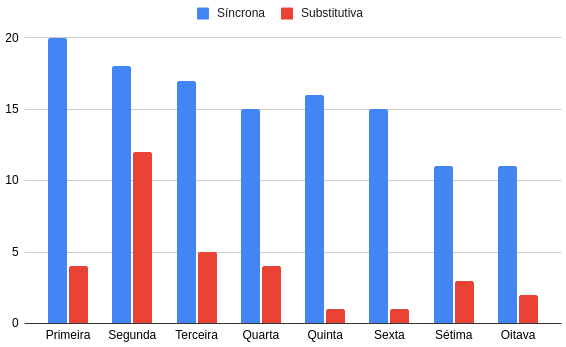
\includegraphics[width=0.7\textwidth]{fig/numerodeatividadesrealizadasORP1.png}
\label{fig:ativsORP1}
\caption*{Fonte: Construção do Autor.}
\end{center}
\end{figure}

A Figura \ref{fig:ativsORP1} que apresenta o gráfico da frequência de atividades entregues na ORP1. Em azul representamos o número de atividades Síncronas que foram entregues pelos alunos, e em vermelho o número de atividades Substitutivas.

Analisando a quantidade de atividades Síncronas entregues, percebemos que apenas na primeira atividade tivemos todos os 20 alunos resolvendo as questões. Vamos salientar aqui que mesmo os alunos que não conseguissem realizar as atividades Síncronas poderiam realizar a atividade Substitutiva.

Caso o aluno optasse por realizar apenas a atividade Substitutiva, ele não sofreria penalidades. A única consequência seria a ausência do \textit{feedback} do tutor para auxiliá-lo. Devido a essa condição, muitos alunos parecem ter escolhido fazer somente a atividade Substitutiva, mesmo que isso resultasse em uma nota máxima menor.

É importante ressaltar novamente que estávamos vivenciando um período de isolamento social, e, nesse contexto, a saúde mental dos estudantes era uma das nossas principais preocupações. Não tínhamos a intenção de impor a todos a realização das atividades Síncronas, uma vez que não tínhamos conhecimento do impacto que essa situação estava causando em cada um deles. O bem-estar dos alunos era prioridade, e compreendíamos que eles poderiam estar enfrentando desafios significativos devido às circunstâncias vigentes.

Entretanto, ao observarmos os dados da Figura \ref{fig:ativsORP1} vemos que, mesmo somando os números de atividades Síncronas e Substitutivas entregues na oitava aplicação, não somamos os 20 alunos que tínhamos no início. Alguns fatores colaboraram para essa diminuição do número de alunos ativos na disciplina.

Em primeiro lugar, é frequente ocorrerem desistências em disciplinas de Física. Muitos estudantes não estão familiarizados com as demandas e exigências do curso. Inclusive, alguns alunos sequer iniciaram o semestre devido à modalidade de ensino remoto adotada.

Em segundo lugar, o impacto da pandemia e do isolamento social afetou significativamente a todos. O tutor relata que alguns alunos expressaram dificuldades em se sentirem aptos a estudar ou realizar as atividades dentro dos prazos estabelecidos, devido a questões de cunho pessoal decorrentes da situação vivenciada.

Em terceiro lugar, alguns estudantes, ao constatarem que já haviam alcançado a nota necessária para aprovação, optaram por redirecionar seu foco para outras disciplinas. É importante ressaltar que, caso um aluno não realizasse uma atividade, sua pontuação correspondente seria atribuída como zero.

\begin{figure}[ht]
\begin{center}
\caption{Gráfico das médias das atividades respondidas da ORP1.}
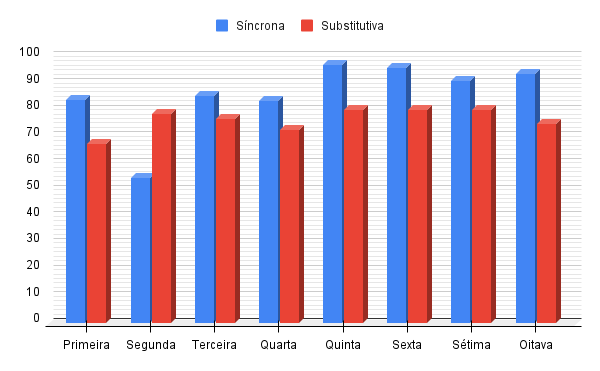
\includegraphics[width=1\textwidth]{fig/mediasORP1.png}
\label{fig:medORP1}
\caption*{Fonte: Construção do Autor.}
\end{center}
\end{figure}

Ao analisar a Figura \ref{fig:medORP1}, podemos obter uma visão geral das médias de cada uma das atividades realizadas pelos alunos. É importante ressaltar que, nesse gráfico específico, foram considerados apenas os valores das pontuações dos alunos que entregaram as atividades dentro do prazo estabelecido.

Com exceção da segunda atividade, em todos os outros casos, a média geral da turma foi maior nas atividades Síncronas. Essa diferença era esperada, visto que a pontuação máxima das atividades Síncronas é maior do que a das atividades Substitutas.

Entretanto, é importante notar que as atividades Substitutivas atingiram o platô em mais de uma ocasião. Isso significa que em diversos momentos, todos os alunos que optaram por realizar as atividades Substitutivas obtiveram nota máxima nessas atividades.

Na segunda atividade, é importante destacar que a média das atividades Substitutivas superou a das atividades Síncronas. Porém, é preciso ter um pouco mais de atenção a esse resultado, pois muitos alunos zeraram a atividade. No entanto, é notável que esses mesmos alunos apresentaram um progresso significativo ao longo da disciplina, obtendo notas cada vez maiores nas demais atividades.

\begin{figure}[ht]
\begin{center}
\caption{Notas finais ORP1.}
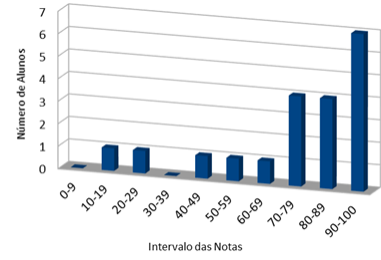
\includegraphics[width=0.8\textwidth]{fig/nfORP1.png}
\label{fig:nfORP1}
\caption*{Fonte: Construção do Autor.}
\end{center}
\end{figure}

Conforme observado nas Figuras \ref{fig:ativsORP1} e \ref{fig:medORP1}, ficou evidente que as atividades Substitutivas cumpriram seu papel de melhorar as notas dos alunos quando necessário. Embora a média geral das atividades Substitutivas seja menor do que a das atividades Síncronas, é importante ressaltar que a média individual dos alunos que optaram pela mudança sempre aumentou. Isso demonstra que as atividades Substitutivas foram efetivas em proporcionar uma oportunidade de melhoria para aqueles que precisavam.

A taxa de aprovação na disciplina foi de aproximadamente 60\%. No entanto, se considerarmos apenas os alunos que interagiram ao longo do semestre, o número sobe para 75\%.

Na Figura \ref{fig:nfORP1}, podemos observar o gráfico das notas finais dos alunos da ORP1. As notas estão divididas em intervalos, onde os alunos que foram aprovados foram aqueles que obtiveram nota igual ou superior a 70. Nota-se uma separação clara entre os alunos que atingiram essa pontuação mínima para aprovação e aqueles que não conseguiram.

A perda dos dados das respostas do questionário comprometeu nossos objetivos de pesquisa, especialmente no que diz respeito à compreensão das formas mais eficientes de dicas para os alunos (objetivo (d)). Devido a essa falta de informações, muitos questionamentos permaneceram vagos e sem respostas claras. A ausência dos dados prejudicou nossa capacidade de analisar de forma abrangente as percepções dos alunos e obter \textit{insights} significativos sobre o impacto do uso das dicas no processo de aprendizagem.

As notas dos alunos demonstraram uma melhora à medida que eles utilizaram o \textit{feedback} nas atividades Substitutivas quando necessário. Além disso, notamos uma redução no número de alunos precisando realizar as Substitutivas à medida que o semestre avançava, pois suas notas nas atividades Síncronas apresentavam um progresso contínuo. Essa correlação sugere que o uso do \textit{feedback} de forma apropriada pode ser um fator-chave para o aprimoramento do desempenho dos alunos e para sua maior eficácia nas atividades avaliativas em tempo real.

Por meio da análise das resoluções dos estudantes, constatou-se que aqueles que fizeram uso do \textit{feedback} durante as atividades Substitutivas exibiram um aprimoramento significativo no processo de RP. Alunos que inicialmente apresentavam dificuldades em extrair informações relevantes das questões, ao término do período letivo, demonstraram habilidade excepcional em resolvê-las com proficiência (objetivo \ref{item:c}).

Com base nisso, verificamos que os alunos adotavam uma abordagem semelhante à estratégia proposta por \citeonline{Pozo2009} ao resolver os problemas. Essa constatação limitou nossa capacidade de obter uma quantidade substancial de informações para a análise do objetivo específico \ref{item:a}.

Ao abordarmos o objetivo \ref{item:b} através das folhas de resposta, evidenciamos duas principais áreas que requerem suporte por parte dos alunos: aprofundamento na análise dos fenômenos físicos e reforço na aplicação prática dos conceitos matemáticos associados. Em muitos casos os alunos não sabiam interpretar a situação descrita pela questão, levando a resultados que não condizem com a realidade.

Além disso, ficamos surpresos com as dificuldades em matemática básica. Os principais erros encontrados envolveram o uso inadequado de operações matemáticas e a falta de habilidade na conversão de unidades. Não esperávamos encontrar tantas dificuldades nesse aspecto em uma turma de Ensino Superior.

Os dados coletados por todos os instrumentos revelaram uma diversidade significativa na turma em relação ao interesse pela RP ao longo do semestre. De fato, observou-se que os alunos demonstraram muito mais interesse em obter aprovação na disciplina do que em se engajar na resolução das atividades propostas.

É confirmado pelo tutor que o objetivo específico \ref{item:b} reflete as informações previamente verificadas pelas outras ferramentas. É nesse contexto que se destaca a maior necessidade de \textit{feedback}, que se concentra principalmente na parte matemática e na análise dos fenômenos descritos.

Entendemos que o objetivo \ref{item:d} não pôde ser totalmente respondido devido às semelhanças entre as dificuldades apresentadas pelos alunos, o que limitou a diversidade dos \textit{feedbacks} fornecidos. Entretanto, durante o processo de análise, surgiu a conscientização da necessidade de desenvolver uma classificação adequada para as dicas a serem utilizadas. Essa etapa é fundamental para garantir uma abordagem mais precisa e eficaz ao fornecer \textit{feedback} aos alunos, permitindo que eles recebam orientações específicas e relevantes para suas necessidades individuais.


\subsection{ORP2} \label{sec:2orp}

Após a conclusão da ORP1, dedicamos um período para estudar e analisar os resultados obtidos. Nesse ínterim, houve uma sinalização de que as aulas presenciais retornariam à UFSM. Diante dessa perspectiva, surgiu a necessidade de realizar um \textit{redesign} em nossa proposta, considerando essa mudança no cenário educacional. Esse processo de \textit{redesign} visa ajustar e adaptar nossa abordagem com base nas novas condições e possibilidades decorrentes do retorno das aulas presenciais, as quais podem impactar a dinâmica de ensino e aprendizagem.

Durante o período de estudos e análise, identificamos a possibilidade de haver diferenças no estilo e padrão de RP entre alunos principiantes e especialistas. Diante dessa constatação, nosso novo \textit{design} foi concebido para abordar duas turmas distintas.

A ORP2 foi aplicada à turma de principiantes, composta por alunos do curso de Licenciatura em Matemática - Noturno, na disciplina de Física II. Apesar de ser o oitavo semestre do currículo, esses alunos foram considerados iniciantes na RP de Física, uma vez que essa era apenas a segunda disciplina deles nessa área específica.

 A escolha da turma de principiantes para a ORP2 ocorreu pelos mesmos motivos da turma da ORP1, ou seja, devido ao fato do professor regente da disciplina também ser o orientador desta dissertação. Essa escolha facilitou a aquisição de informações e dados em um contexto geral da disciplina, permitindo uma abordagem mais detalhada e abrangente sobre a RP de Física nessa turma específica.

A Tabela \ref{tab:aplORP} revela que tivemos um número reduzido de apenas 3 alunos matriculados na turma. Apesar de não termos conhecimento antecipado desse baixo número de alunos, decidimos manter nossa forma de atuação conforme previamente estruturada na Seção \ref{sec:orp2e3}. Essa decisão foi tomada visando oferecer a melhor experiência possível aos alunos, garantindo que aqueles que se matricularam na disciplina recebessem o suporte e o acompanhamento necessário para o seu aprendizado e progresso acadêmico.

Durante as intervenções, o autor desta dissertação assumiu o papel de tutor da turma, responsável por auxiliar os alunos em suas dúvidas e fornecer as dicas necessárias para que alcançassem o progresso esperado nas questões. Como tutor, sua função era estar disponível para orientar os estudantes em seus estudos, esclarecer conceitos e oferecer suporte durante todo o processo de aprendizagem. Além disso, o tutor tinha a tarefa de fornecer as dicas apropriadas para ajudar os alunos a resolverem os desafios propostos, visando aprimorar seu desempenho nas atividades propostas. 

O livro utilizado como material didático na disciplina foi o "Fundamentos de Física", volume 2, de \citeonline{Halliday2009vol2}. A escolha desse livro foi motivada pelo fácil acesso dos estudantes, uma vez que o livro fazia parte da biblioteca virtual da instituição. Embora o ensino estivesse sendo retomado de forma presencial, a disponibilidade do livro digital facilitava o acesso dos alunos ao conteúdo, uma vez que a demanda pelos exemplares impressos era alta e poderia dificultar a retirada nas dependências da biblioteca.

Além disso, a escolha deste livro foi motivada pelo fato de ele utilizar o mesmo sistema de classificação de dificuldade das questões descrito na Tabela \ref{tab:halliday_dificuldade}. Isso possibilitou ao tutor montar as listas de questões, garantindo que nelas constassem apenas problemas, e não exercícios. Essa abordagem permitiu um maior enfoque em desafios conceituais e práticos, promovendo o desenvolvimento das habilidades dos estudantes na resolução de problemas complexos e na compreensão dos fundamentos da Física.

Na aplicação, os alunos resolveram as listas de exercícios em aula, na presença do tutor, e não nos preocupamos com possíveis cópias de resolução. A turma não era grande, o que facilitou o acompanhamento individualizado e tornou o controle sobre as cópias mais viável. A abordagem colaborativa proporcionou uma interação mais próxima e efetiva entre os estudantes e o tutor.

Foram aplicadas cinco listas de questões, detalhadas no Apêndice \ref{apendice:asa2}. Durante o início do processo, enfrentamos a dificuldade de selecionar o número ideal de questões a serem incluídas em cada lista. 

A primeira lista foi elaborada com 11 questões, com o intuito de abordar ao menos um problema representativo de cada tópico do capítulo trabalhado. Essa abordagem foi planejada para garantir que os alunos tivessem a oportunidade de praticar diferentes habilidades e conceitos abordados na disciplina, proporcionando uma visão geral dos temas tratados.


Durante a aplicação da primeira lista, identificamos que o tempo necessário para os alunos resolverem as questões era excessivamente longo. Os estudantes levaram cerca de 5 aulas para concluir a tarefa, o que estava além do tempo ideal, que seria de no máximo 2 aulas.

Compreendemos que a dificuldade enfrentada pelos alunos na resolução da lista estava relacionada tanto à própria natureza da RP em Física, uma vez que se tratava de uma turma de iniciantes nesse tipo de abordagem, quanto à quantidade de questões presentes na lista.

Dado que a turma era formada por estudantes novos na prática da RP, era natural que enfrentassem desafios em sua execução. No entanto, ao identificar que o número de questões também contribuía para o tempo excessivo de resolução, tomamos a decisão de reduzir a quantidade de questões nas próximas listas.

Essa abordagem visava proporcionar aos alunos uma experiência mais focada e menos sobrecarregada, permitindo-lhes dedicar mais tempo e atenção a cada problema apresentado. Acreditamos que essa adaptação contribuirá para que os estudantes se envolvam mais profundamente com cada tarefa, alcançando maior compreensão dos conceitos e desenvolvimento das habilidades em RP de Física.

Para otimizarmos o tempo de resolução das listas, decidimos por reduzir o número de questões em cada lista para 4. Essa escolha foi baseada em proporcionar aos alunos uma abordagem mais eficiente e focada, permitindo que dedicassem maior atenção e aprofundamento em cada problema apresentado.

As questões foram selecionadas cuidadosamente pelo tutor, visando englobar os pontos mais relevantes dos capítulos trabalhados, abordando diferentes conceitos e estratégias de resolução. Dessa forma, buscamos oferecer uma variedade de desafios que não se repetissem, promovendo um aprendizado mais abrangente e diversificado para os estudantes.

A execução da primeira lista de questões evidenciou uma dificuldade significativa por parte dos alunos em estabelecer conexões entre seus conhecimentos matemáticos e a aplicação desses conceitos nas questões de Física propostas. Esse cenário revelou a importância de trabalhar de forma mais gradual e cuidadosa na transição entre a teoria matemática e sua aplicação na RP de Física.

Diante dessa percepção, decidimos fornecer aos alunos algumas questões mais simples, envolvendo um círculo, com o objetivo de auxiliá-los a se familiarizar e se acostumar com o processo de RP de Física. Essas questões serviram como uma ponte para conectar os conceitos matemáticos aprendidos anteriormente às situações práticas e reais propostas nas questões de Física.

Essa abordagem foi fundamental para criar uma base sólida e confiante nos alunos, permitindo que eles desenvolvessem gradualmente a capacidade de utilizar seus conhecimentos matemáticos de forma eficiente na RP de Física. Ao longo do semestre, esse enfoque gradual possibilitou um progresso significativo nos resultados dos alunos e melhorou sua compreensão e confiança na abordagem de questões mais complexas de Física.

Ao longo do semestre, foram aplicadas cinco listas de problemas, cada uma correspondente a um capítulo do livro adotado. Dos três alunos matriculados na disciplina, apenas um deles acabou reprovando. Essa reprovação ocorreu antes mesmo do término do semestre, pois o estudante enfrentou dificuldades para comparecer regularmente às aulas.

A situação do estudante em questão parece ter sido afetada por problemas de disponibilidade de horários, o que o levou a não conseguir acompanhar as aulas regularmente. Infelizmente, essa ausência constante acabou impactando negativamente seu desempenho acadêmico, resultando na reprovação na disciplina.

É importante ressaltar que as intervenções realizadas durante o semestre buscavam auxiliar os alunos no desenvolvimento das habilidades necessárias para a RP de Física e, ao mesmo tempo, levar em consideração as particularidades e dificuldades individuais de cada estudante. Apesar do resultado negativo de um dos alunos, é possível observar que houve uma taxa de aprovação foi de aproximadamente 67\% (2 de 3 alunos), considerando a reprovação mencionada anteriormente.

Compreendemos as limitações impostas pela pequena quantidade de alunos na turma, o que pode ter afetado a confiabilidade dos resultados obtidos e limitado a capacidade de resposta aos objetivos do trabalho. É importante reconhecer que a amostra reduzida pode impactar a generalização dos resultados e dificultar a obtenção de conclusões mais abrangentes.

A turma com poucos alunos pode ter sido uma surpresa e, como fora mencionado anteriormente, não houve conhecimento prévio desse fato. Essa característica da turma pode ter influenciado os resultados obtidos, uma vez que a variabilidade dos dados pode ser menor, tornando mais difícil identificar padrões significativos.

No entanto, é essencial considerar que a realização da pesquisa e a coleta de dados são etapas importantes para o avanço do conhecimento científico. Mesmo que os resultados não tenham atingido a confiabilidade desejada, o trabalho realizado pode servir como ponto de partida para futuras investigações e aprimoramentos no campo de estudo.


No próximo \textit{redesign}, é fundamental reconhecer e mencionar as limitações do estudo, principalmente o tamanho da amostra. Uma turma composta por poucos alunos pode impactar os resultados, limitando a generalização dos achados. Para obter uma compreensão mais abrangente do tema, é importante buscar formas de superar essas limitações.

\subsection{ORP3} \label{sec:3orp}

A ORP3 foi realizada de forma concomitante à ORP2, com ambas utilizando o mesmo processo de avaliação. Os alunos foram avaliados por meio de listas de exercícios que deveriam ser resolvidas durante as aulas. Além disso, o andamento da disciplina dependia diretamente da evolução dos alunos nas atividades propostas.

Esse formato de avaliação em sala de aula permitiu um acompanhamento mais próximo do progresso dos estudantes, possibilitando ao tutor identificar eventuais dificuldades e fornecer o suporte necessário para o aprendizado. A abordagem de resolução de listas durante as aulas pode ter contribuído para o engajamento dos alunos, já que as dúvidas puderam ser sanadas de imediato e os conceitos aplicados de forma prática.

Dessa forma, a metodologia utilizada nas Oficinas proporcionou uma interação mais dinâmica entre tutor e alunos, permitindo uma avaliação mais precisa do conhecimento adquirido e a adaptação das estratégias de ensino conforme a necessidade da turma. Essa abordagem pode ter favorecido o aprendizado e o engajamento dos alunos ao longo da disciplina.

Na ORP3, a disciplina abordada foi Mecânica Quântica I, ministrada no sétimo semestre do curso de Física. Nessa etapa do curso, consideramos os acadêmicos como especialistas na RP de Física, uma vez que estavam prestes a concluir a graduação em Física.

A escolha de Mecânica Quântica I como disciplina para a ORP3 também foi influenciada por questões de conveniência e praticidade. O fato de o orientador desta dissertação atuar novamente como professor regente da disciplina possibilitou um acesso mais fácil e direto às turmas, permitindo uma maior integração e colaboração entre o professor e o autor deste trabalho, que desempenhava o papel de tutor.

A proximidade entre o professor regente e o tutor pode ter proporcionado uma melhor coordenação e alinhamento das atividades da disciplina com os objetivos da pesquisa em RP de Física. A atuação conjunta desses dois papéis também pode ter facilitado a identificação e seleção das questões mais relevantes e desafiadoras para as listas, garantindo uma abordagem mais efetiva na promoção do desenvolvimento das habilidades de resolução de problemas dos estudantes.

Na aplicação da ORP3, assim como na ORP2, também nos deparamos com um baixo número de estudantes matriculados. Apesar disso, decidimos manter o padrão de aplicação previamente desenvolvido, visando realizar uma análise comparativa mais consistente entre as duas turmas.


Na disciplina de Mecânica Quântica I, mesmo sendo uma disciplina avançada na graduação de Física, foi preciso realizar uma revisão de alguns princípios de Física Moderna com os estudantes. Para esse propósito, optamos pelo livro "Fundamentos de Física", volume 4, de \citeonline{halliday}, pelas mesmas razões já mencionadas para as ORP1 e ORP2. Essa abordagem permitiu reforçar conceitos fundamentais e nivelar o conhecimento dos alunos, proporcionando uma base mais sólida para o aprofundamento nos conteúdos de Mecânica Quântica.

Portanto, a primeira lista de questões na disciplina de Mecânica Quântica I teve como foco a revisão dos princípios da Física Moderna (Apêndice \ref{ch:orp3l1}). Semelhante à ORP2, que ocorria concomitantemente, observamos a necessidade de reduzir o número de questões para otimizar o tempo de resolução e proporcionar aos alunos uma abordagem mais eficiente e aprofundada em cada problema proposto.

A primeira lista abrangia 10 problemas para serem resolvidos, e os alunos levaram aproximadamente 3 semanas para completá-la. Após discussões com o professor regente, concordamos em reduzir o número de questões nas próximas listas, limitando-as a, no máximo, 4 problemas. 

Ao contrário da ORP2, onde as listas foram fixadas em 4 questões, na ORP3 optamos por deixar esta margem para o tutor na escolha do número de questões. Essa decisão foi tomada devido à natureza das questões da disciplina, que requeriam mais tempo, conhecimento e concentração por parte dos alunos. Dessa forma, permitimos ao tutor ajustar o número de problemas de acordo com a complexidade e abrangência dos tópicos abordados em cada lista, proporcionando uma melhor adaptação às necessidades da turma.

Para prosseguir com o andamento da disciplina e abordar os conteúdos próprios da Mecânica Quântica, o professor regente optou por utilizar o livro "Física Quântica" de \citeonline{Gasiorowicz1979}. Essa escolha ocorreu por acreditarmos que os alunos estariam preparados para enfrentar um material tecnicamente mais robusto.


Com base nas dificuldades encontradas ao tentar resolver algumas questões com os alunos em sala de aula, o professor regente percebeu que eles apresentam muita dificuldade em aspectos matemáticos. Diante disso, a utilização do livro de \citeonline{Gasiorowicz1979} poderia acabar prejudicando o desenvolvimento dos alunos. É importante considerar que a abordagem de um material mais avançado requer uma base sólida em matemática, e é fundamental garantir que os estudantes estejam devidamente preparados para enfrentar os desafios da Mecânica Quântica.

Após uma cuidadosa análise do professor e do tutor, optamos por adotar o livro "Mecânica Quântica" de \citeonline{Griffiths2011} como material principal para a disciplina. Essa escolha foi motivada pelas dificuldades dos alunos em relação aos aspectos matemáticos encontrados ao tentar resolver algumas questões com eles em sala de aula.

O livro de \citeonline{Griffiths2011} oferece uma abordagem mais moderna e clara, além de contar com questões complementares que enriquecem o aprendizado. Acreditamos que essa nova opção nos permitiria traçar um processo de ensino e aprendizagem mais simples e eficiente, auxiliando os alunos a superarem suas dificuldades e progredirem de maneira mais consistente no estudo da Mecânica Quântica.

Após a adoção do novo material, que ocorreu na primeira metade do semestre, foram aplicadas mais duas listas de exercícios (Apêndices \ref{ch:orp3l2} e \ref{ch:orp3l3}). Diferentemente do que ocorreu na ORP2, onde os alunos conseguiam realizar as listas dentro de uma ou duas aulas, os estudantes na ORP3 continuaram precisando de mais tempo para resolver as questões.

Entendemos que os alunos tenham apresentado a necessidade de trabalhar e tenham muitas obrigações fora da sala de aula, o que pode impactar diretamente o tempo disponível para estudar e resolver as listas de exercícios. Essa é uma realidade comum em muitos ambientes acadêmicos, e é importante levar em consideração os diversos compromissos e responsabilidades que os estudantes enfrentam.

Os alunos faziam questionamentos pertinentes ao tutor, mostrando que eles estavam engajados e interessados em aprender, buscando compreender os conceitos de forma mais aprofundada. No entanto, é natural que a RP, especialmente em uma disciplina complexa como a Mecânica Quântica, demande tempo e dedicação.

Para auxiliar os alunos nesse processo e permitir a continuação das aulas teóricas, decidimos permitir que os alunos entregassem algumas listas de forma remota. No entanto, para evitar plágios e garantir a integridade do processo de resolução, o tutor precisaria verificar o progresso individual de cada aluno, assegurando que cada resposta fosse original e resultado do esforço individual. 

Ao final do semestre, o comprometimento e esforço dos estudantes foram recompensados com a aprovação. No entanto, assim como na ORP2, a quantidade limitada de dados disponíveis para análise nos impediu de realizar uma análise mais abrangente dos objetivos propostos. 

Podemos observar alguns pontos em comum entre as ORP2 e ORP3. Ambas as turmas apresentaram um número reduzido de alunos, o que impactou na aplicação da proposta inicial. No entanto, mesmo com esse cenário, foi possível notar a participação ativa dos estudantes durante as aulas, com questionamentos pertinentes e interesse nas atividades propostas (segundo a análise do tutor). É importante ressaltar que, devido à limitação de dados, é necessário cautela ao interpretar quaisquer resultados, pois a falta de uma amostra maior pode comprometer a representatividade dos achados. 

\section{Aplicações das ASA}


Diante das dificuldades enfrentadas nas ORP2 e ORP3, bem como os problemas técnicos na coleta de dados na ORP1, foi necessário repensar nossas estratégias para obter resultados mais expressivos e consistentes. Para isso, uma abordagem promissora foi o aumento do tamanho das turmas, visando coletar dados de um maior número de alunos e tornar as análises mais confiáveis e representativas.

Compreendendo as dificuldades e desafios enfrentados no primeiro semestre de retorno às aulas presenciais, em que o Ensino Superior ainda sofria com os reflexos da alta evasão decorrente da Pandemia \cite{Palhares2022}, decidimos repensar nosso público-alvo para obter resultados mais consistentes e significativos. Diante da incerteza quanto ao crescimento do número de estudantes nas turmas de Ensino Superior, optamos por direcionar nossas intervenções para o Ensino Médio, onde já possuíamos conhecimento do número mais elevado de alunos.

As intervenções realizadas no Ensino Médio foram denominadas de ASA e são detalhadas na Seção \ref{sec:asa}. Ao contrário das ORP, que tinham a duração de um semestre, as ASA foram planejadas para serem aplicadas em um trimestre, devido à divisão dos períodos letivos na instituição. Essa alteração no cronograma permitiu um enfoque mais concentrado nas atividades e uma maior agilidade na coleta de dados e análise dos resultados. 

As ASA foram aplicadas durante os meses de março, abril e maio de 2023. Cada turma participou de três atividades ao longo desse período, com um espaçamento médio de um mês entre cada atividade. Cada uma dessas atividades consistia em quatro modelos (variações) distintas, propostas para dificultar plágio entre as resoluções dos alunos.

A decisão de direcionar nossas intervenções para o Ensino Médio foi facilitada pelo fato de o autor desta dissertação ser o professor regente das turmas selecionadas. Assim, a pesquisa foi realizada em uma Escola Particular Confessional no interior do Estado do Rio Grande do Sul, contemplando três turmas correspondentes a cada ano do Ensino Médio.

Compreendemos que a troca para o público-alvo do Ensino Médio, e consequentemente a inclusão de alunos de diferentes anos, impediu a análise específica das diferenças no processo de RP entre estudantes principiantes e experientes. De fato, essa abordagem permitiria investigar se os alunos mais velhos (do terceiro ano) demonstrariam maior habilidade e destreza na resolução de problemas, em comparação aos alunos de anos anteriores.

No entanto, é importante considerar que as dificuldades apresentadas pelas turmas, mesmo aquelas com alunos mais velhos, podem ser influenciadas pelas experiências de aprendizagem prévias em ambientes remotos. A transição para o ensino remoto durante o período de pandemia parece ter gerado desafios adicionais para os estudantes, como o acesso limitado aos recursos educacionais, a falta de interação presencial com os colegas e professores, e a adaptação a novas plataformas e metodologias de ensino \cite{Santos_Bastos_Souza_Figueiredo_Teixeira_Quintiliano_2021}.

\begin{table}[ht]
\centering
\caption{Informações básicas das turmas de aplicação das ASA.}
\label{tab:basicoASA}
\begin{tabular}{p{5cm}rrr}
\toprule
& \textbf{ASA1} & \textbf{ASA2} & \textbf{ASA3} \\
\midrule
\textbf{Alunos na Turma} & 24 & 26 & 19 \\
\textbf{Alunos Avaliados} & 16 & 21 & 14 \\
\textbf{Média de Idade (anos)} & 15 & 16 & 17 \\
\bottomrule
\end{tabular}
\caption*{Fonte: Construção do Autor.}
\end{table}

A Tabela \ref{tab:basicoASA} apresenta informações fundamentais sobre as turmas nas quais aplicamos as ASA. Nela, podemos observar que há variações na quantidade de alunos matriculados em cada turma, bem como nos alunos que efetivamente participaram das avaliações durante a aplicação das atividades. 

Entendemos que a discrepância na quantidade de alunos nas turmas que participaram das ASA pode ser atribuída a diferentes fatores. Dois dos principais motivos são o critério de considerar apenas os alunos que realizaram todas as atividades junto com a turma, bem como a presença de estudantes com laudos médicos que requerem acompanhamento e avaliações especiais. Essa abordagem visa manter a consistência na análise dos resultados, uma vez que a participação regular nas atividades é fundamental para avaliar o impacto das ASA na aprendizagem dos alunos.

Nas Seções \ref{subsec:asa1}, \ref{subsec:asa2} e \ref{subsec:asa3}, realizaremos uma análise individual das aplicações das ASA em cada uma das turmas do Ensino Médio. Ao final de cada seção, faremos uma conexão entre os dados obtidos nessas aplicações e os objetivos do trabalho proposto.

Adicionalmente, considerando que o professor regente (autor desta dissertação) já havia lecionado para as turmas anteriormente, é relevante fornecer um breve histórico sobre cada uma delas. Essa abordagem inédita no presente trabalho foi considerada benéfica, pois possibilitou utilizar essas informações na formulação do \textit{design} atual da pesquisa.

\subsection{ASA1} \label{subsec:asa1}

A ASA1 foi aplicada em uma turma de 1º ano do Ensino Médio. Conforme apresentado na Tabela \ref{tab:basicoASA}, a turma possuía um total de 24 alunos, mas para fins desta pesquisa, foram considerados apenas 16 deles. A escolha de excluir alguns alunos da análise se deveu a critérios específicos, como a participação em todas as atividades propostas e a presença de laudos médicos\footnote{Existiam alunos que eram diagnosticados com transtornos e dificuldades de aprendizagem, o que exigia uma avaliação adaptada para os mesmos. Estes alunos foram avaliados mas não foram considerados no estudo, pois suas atividades diferiam do restante dos estudantes analisados.} que pudessem interferir na proposta do estudo. 

O tutor já havia lecionado Matemática para esta turma no ano anterior, quando eles estavam no 9º ano do Ensino Fundamental II. Durante a transição para o Ensino Médio, a turma sofreu com a saída de muitos alunos, e os novos estudantes que ingressaram não compensaram essas perdas, resultando em um número menor de alunos na turma.

Durante o período de transição, alguns alunos ingressaram na turma apresentando laudos médicos e condições especiais, o que não era comum anteriormente. Esses estudantes acabaram por gerar desafios adicionais, pois suas necessidades requeriam um acompanhamento diferenciado e, em algumas situações, tumultuavam o ambiente durante as aulas.

A turma do 9º ano já apresentava desafios significativos em termos de disciplina e dificuldades de aprendizagem. Com a chegada dos novos alunos no Ensino Médio, essas questões foram agravadas, tornando o trabalho com a turma ainda mais desafiador. O ambiente de sala de aula se mostrou complexo devido à presença mais frequente de comportamentos disruptivos.

É importante ressaltar que esses estudantes enfrentaram condições de ensino adversas durante a Pandemia. No 7º ano, as aulas foram realizadas de forma remota, e no 8º ano, em formato híbrido. Essa transição entre modalidades de ensino pode ter afetado o engajamento e o desempenho dos alunos. Além disso, no 9º ano, houve uma flexibilização em relação às faltas na escola, considerando as dificuldades de adaptação dos estudantes durante esse período desafiador. Esses fatores podem ter contribuído para a dinâmica complexa da turma no Ensino Médio.

Com base nos desafios enfrentados durante o Ensino Fundamental e na possível falta de aprofundamento em conceitos matemáticos essenciais, é compreensível que esses estudantes tenham chegado ao Ensino Médio com lacunas em seu processo de formação. Essas lacunas podem refletir em maiores dificuldades no aprendizado da Física.

Ao considerar as dificuldades e particularidades da turma, a formulação das atividades foi cuidadosamente planejada para atender às necessidades dos alunos. Esperamos que nossos achados e observações estejam alinhados com o contexto histórico dessa turma, possibilitando uma análise mais abrangente e significativa dos resultados obtidos durante a aplicação das atividades. 

As atividades que compuseram a ASA1 estão detalhadas no Apêndice \ref{apendice:asa1}. Neste apêndice, são apresentadas as três aplicações da ASA1, incluindo os diferentes modelos utilizados para reduzir a possibilidade de plágio por parte dos alunos.

Para a descrição dos eventos específicos de cada intervenção, utilizaremos informações contidas na Figura \ref{fig:dicasASA1}. Nela, estão representados, por aplicação, os tipos de dicas mais solicitadas. Esta mesma Figura será utilizada ao final desta seção para a análise do comportamento geral da turma em relação aos diversos tipos de dicas.

\begin{figure}[ht]
\begin{center}
\caption{Gráfico das dicas solicitadas ao longo da ASA1.}
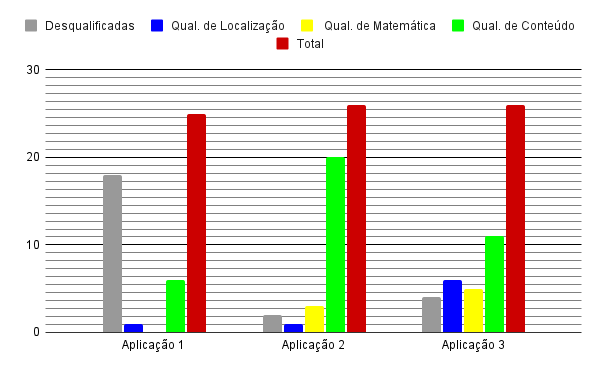
\includegraphics[width=1\textwidth]{fig/graficoDicasASA1.png}
\label{fig:dicasASA1}
\caption*{Fonte: Construção do Autor.}
\end{center}
\end{figure}

A  aplicação 1 (Apêndice \ref{ch:ASA1a1}) abordou o conteúdo de cinemática escalar. Durante as aulas, os alunos aprenderam sobre as convenções e construção dos sistemas de coordenadas, bem como o cálculo de velocidade e aceleração média. O conteúdo incluiu definições de deslocamento, distância percorrida e trajetória.

Foram realizados exercícios em sala de aula, muito semelhantes ao fornecido durante a  aplicação 1. Por esse motivo, supomos que os alunos não teriam dificuldade em resolver essa atividade.

Quando analisamos a Figura \ref{fig:dicasASA1}, podemos observar que a maioria dos questionamentos (72\%) feitos durante a aplicação 1 foram classificados como dúvidas desqualificadas. Isso indica que os alunos, ao encontrarem dificuldades, não sabiam como iniciar o processo para esclarecer suas dúvidas e prosseguir na RP.

A identificação de uma grande proporção de alunos solicitando dúvidas desqualificadas após a aplicação 1 revelou um quadro preocupante de dificuldades na compreensão do conteúdo. Diante desses resultados, o professor promoveu um diálogo com a turma para entender as razões por trás dessa dificuldade generalizada. A maioria dos alunos relatou não ter compreendido o conteúdo ministrado.

A constatação de que mais de um mês havia se passado desde o início do ano letivo quando a aplicação 1 foi realizada levou o professor a questionar os alunos sobre o quanto eles haviam estudado o conteúdo em casa nesse período. Surpreendentemente, muitos alunos admitiram não terem dedicado tempo suficiente aos estudos fora da sala de aula. Além disso, o professor percebeu que os alunos não o procuravam para tirar dúvidas, mesmo quando ele questionava em sala de aula sobre suas dificuldades. Esses aspectos levantaram preocupações sobre a necessidade de reforçar a importância do estudo individual e da busca ativa por esclarecimento de dúvidas para o progresso dos alunos.

Após o diálogo com os alunos, houve um compromisso por parte deles de se esforçarem mais no estudo individual, tanto na escola quanto em casa. Esse comprometimento refletiu diretamente nas aplicações 2 e 3 da ASA1, conforme ilustrado na Figura \ref{fig:dicasASA1}, onde o número de dúvidas desqualificadas diminuiu significativamente.

Dentro da aplicação 1, é importante mencionar os alunos que não solicitaram dicas ao professor durante a resolução das atividades. Nesse contexto, observou-se que 4 alunos optaram por não buscar ajuda, e, preocupantemente, apenas 1 desses estudantes conseguiu resolver corretamente a questão proposta.

De fato, a ausência de solicitação de dicas por parte de alguns alunos durante a resolução das atividades pode ser um indicativo de diferentes problemas. Como mencionado, isso pode sugerir que o aluno não tem clareza sobre como abordar o problema, pode demonstrar falta de interesse ou motivação para resolver a questão, ou até mesmo uma possível confiança excessiva em suas habilidades que leva a erros na resolução. Essas questões são preocupantes, pois podem impactar negativamente o desempenho do aluno e sua aprendizagem. 

Na aplicação 2 (Apêndice \ref{ch:ASA1a2}), trabalhamos especificamente o conceito de movimento retilíneo uniforme, considerando as dificuldades que os alunos tiveram com o conceito de velocidade na aplicação 1. Nosso objetivo era analisar os progressos dos alunos, inclusive no compromisso de estudarem em casa, por meio dessa abordagem mais focada.

Como já mencionado anteriormente, o número de dicas desqualificadas reduziu em relação à aplicação 1. No entanto, nessa etapa, surgiram dúvidas relacionadas tanto a conceitos matemáticos quanto a conteúdo específico da Física.

As dúvidas de origem Matemática estavam relacionadas à dificuldade dos alunos em montar uma função que relacionasse os dados fornecidos. Embora tenham sido apenas 3 dúvidas dessa natureza, é importante ficar atento ao fato de os alunos não conseguirem utilizar uma ferramenta matemática tão básica para a resolução dos problemas propostos.

As dúvidas de Conteúdo estavam relacionadas às formas de conversão de unidades e ao cálculo da distância a ser percorrida. Em muitos casos, essas perguntas surgiram ao mesmo tempo, o que indica uma dificuldade dos alunos em separar dois conceitos físicos distintos. A falta de clareza na compreensão desses conceitos pode ter contribuído para as dúvidas e dificuldades enfrentadas pelos alunos durante a resolução dos problemas. 

Nesta aplicação, constatamos que 6 alunos não solicitaram dicas ao professor, e, infelizmente, apenas 1 desses estudantes conseguiu acertar a questão. Esse mesmo aluno havia acertado a questão anterior na aplicação 1 sem precisar de dicas. 

A persistência do mesmo aluno em acertar a questão na aplicação 2, sem solicitar dicas ao professor, pode indicar que ele possui um bom domínio do conteúdo abordado e está mais confiante em suas habilidades. No entanto, é preocupante que os demais alunos que não solicitaram dicas também não tenham acertado a questão.

Na aplicação 3 (Apêndice \ref{ch:ASA1a3}), abordamos os conceitos de movimento retilíneo uniforme e movimento retilíneo uniformemente variado simultaneamente. Os alunos foram desafiados a resolver o problema que requeria uma boa compreensão desses tópicos, bem como o conceito de independência dos eixos no movimento.

Com base nas dificuldades enfrentadas nas atividades anteriores e na complexidade dos conceitos abordados, previmos que haveria uma distribuição mais equilibrada das solicitações de diferentes tipos de dicas na aplicação 3. Observando a Figura \ref{fig:dicasASA1} vemos que essa tendência se confirma.

É importante enfatizar a redução nas solicitações de dicas de Conteúdo e o aumento das dicas de Localização na aplicação 3. Esses dois tipos de dicas apresentaram a maior variação ao longo de todo o processo da ASA1.

Na aplicação 3, as dicas de Localização estão associadas ao fato de os alunos confundirem o movimento retilíneo uniforme com o movimento uniformemente variado. Além disso, esses mesmos estudantes apresentaram dúvidas de Conteúdo, demonstrando dificuldade em relacionar os dois tipos de movimento abordados na questão.

As dúvidas de Conteúdo foram, em sua maioria, associadas à forma e ao uso das equações dos movimentos. Apesar de receberem essas informações, os alunos continuavam apresentando dificuldades na resolução da questão.

Na última etapa da ASA1, tivemos 7 alunos que não solicitaram dicas. Dos alunos que não pediram dicas, 2 acertaram a questão. Um dos alunos foi o mesmo que acertou sem dicas nas duas aplicações anteriores, enquanto o outro não havia solicitado dicas e também não havia acertado nenhuma questão anteriormente.

O progresso do aluno mesmo sem o uso de dicas na última aplicação é notável. Ao conversar com ele, o professor descobriu que o estudante estava passando por problemas pessoais que o afetaram no início do período letivo.

\begin{table}[ht]
\centering
\caption{Principais perguntas dos alunos durante a ASA1.} \label{tab:pergASA1}
\begin{tabular}{c|c}
\hline
\textbf{Pergunta} & \textbf{Classificação}\\ \hline
Como identifico o tipo de movimento? & Localização\\ 
Como inicio a resolução da questão? & Desqualificada \\ 
Como calculo a distância percorrida? & Conteúdo \\
Qual é a equação da velocidade média? & Conteúdo \\
O tempo total é a soma dos tempos de cada etapa? & Conteúdo \\
Qual a fórmula que uso para converter a unidade da velocidade? & Conteúdo \\
\hline
\end{tabular}
\caption*{Fonte: Construção do Autor.}
\end{table}


Por fim, na Tabela \ref{tab:pergASA1} temos alguns exemplos das perguntas que foram mais repetidas pelos alunos ao longo de todo o processo de aplicação da ASA1. Esses questionamentos recebem a mesma classificação que o tipo de dica utilizada para respondê-los.

\subsubsection{Considerações Gerais da ASA1} \label{subsubsec:asa1}

Até o momento, foram apresentadas as principais características de cada aplicação da ASA1. No entanto, para alcançar uma abordagem mais abrangente, é essencial realizar uma análise integrada das três aplicações, a fim de possibilitar avaliações de qualidade. Essa análise conjunta permitirá compreender o comportamento coletivo da turma, considerando os diferentes tipos de dicas solicitadas e o desempenho dos alunos ao longo do processo.

Inicialmente, é essencial discutirmos o conteúdo das folhas de resolução dos alunos, como mencionado anteriormente na Seção \ref{sec:asa}. Esse objeto de estudo está diretamente relacionado ao objetivo \ref{item:a}.

É importante destacar que as aplicações da ASA1 representaram as primeiras experiências dos alunos em RP de Física. Nesse contexto, não tínhamos expectativas de que as respostas estivessem inicialmente bem organizadas e estruturadas. O processo de aquisição de habilidades em RP demanda tempo e prática, e é natural que os estudantes enfrentem dificuldades iniciais na abordagem dessas questões.

A análise das folhas revelou que, ao longo do período letivo, a maioria dos estudantes ainda apresentava dificuldades em organizar suas ideias para as resoluções dos problemas. Esse cenário ficou evidente pelo aumento no número de dicas desqualificadas na aplicação 3, indicando que os alunos continuavam a enfrentar obstáculos para progredir na resolução das questões de forma autônoma.

\begin{figure}
    \centering
    \caption{Exemplo de Organização ASA1.}
    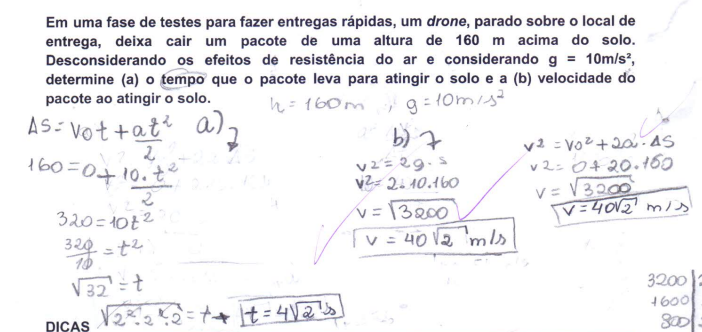
\includegraphics[width=1\textwidth]{fig/orgasa1.png}
    \caption*{Fonte: Extraído da produção dos Estudantes.}
    \label{fig:orgasa1}
\end{figure}

Os alunos que conseguiam estruturar suas ideias apresentaram respostas mais organizadas e claras em suas folhas de resolução (Figura \ref{fig:orgasa1}). Suas abordagens permitiam uma compreensão clara dos dados fornecidos, do questionamento apresentado e das estratégias adotadas para a resolução do problema. Esse padrão demonstra que esses alunos conseguiram articular de forma eficiente seus pensamentos, evidenciando uma maior capacidade de comunicação e coerência em suas respostas.

É relevante destacar que os alunos capazes de estruturar mais efetivamente seus pensamentos foram os mesmos que buscaram as dicas qualificadas. Esse fato evidencia uma correlação positiva entre a organização escrita e o raciocínio dos estudantes. Indica que os estudantes com resoluções mais bem organizadas também demonstraram uma propensão maior a solicitar orientações específicas, sugerindo uma abordagem mais sistemática e estratégica na RP.

Os alunos que foram capazes de resolver as questões mostraram-se proficientes em estruturar suas ideias e expressá-las por escrito. Eles começaram o processo anotando os dados e incógnitas relevantes e, em seguida, identificando quais partes do conteúdo estudado poderiam auxiliá-los na resolução do problema, avaliando a necessidade de solicitar dicas. 

A abordagem dos alunos ao resolver os problemas se assemelha significativamente aos procedimentos descritos por \citeonline{Pozo2009}. De fato, esses passos têm se mostrado uma forma eficiente de abordar a RP de Física. A organização das ideias e a identificação dos dados relevantes são elementos cruciais para um raciocínio claro e estruturado na busca de soluções em Física.

A análise das dicas fornecidas aos alunos foi escolhida para verificar o objetivo \ref{item:b}, uma vez que essas dicas foram categorizadas em quatro tipos distintos, conforme descrito na Seção \ref{sec:asa}. Essa abordagem permitiria identificar em quais momentos as ajudas foram mais relevantes, fornecendo informações sobre os pontos em que os estudantes apresentaram maior dificuldade e necessidade de orientação adicional.

Durante a realização da ASA1, um total de 77 dicas foram fornecidas aos alunos. Dessas dicas, 24 foram classificadas como desqualificadas, 8 como dicas de Localização, 8 de Matemática e 37 de Conteúdo. 

As expectativas iniciais apontavam para uma maior frequência de solicitações de dicas de Matemática, devido às dificuldades decorrentes da Pandemia. No entanto, observou-se que as dicas mais solicitadas pelos alunos foram as de Conteúdo e as classificadas como desqualificadas.

A análise dos resultados e as observações do professor indicam que os alunos enfrentaram uma maior dificuldade na compreensão das questões propostas. A Figura \ref{fig:difasa1} exemplifica a dificuldade de alguns alunos. Essa dificuldade foi evidenciada pelo fato de que, na maioria dos casos, os estudantes não conseguiram avançar para a etapa de aplicação dos conhecimentos e procedimentos matemáticos na resolução dos problemas. 

\begin{figure}
    \centering
    \caption{Dificuldade de resolução -  ASA1.}
    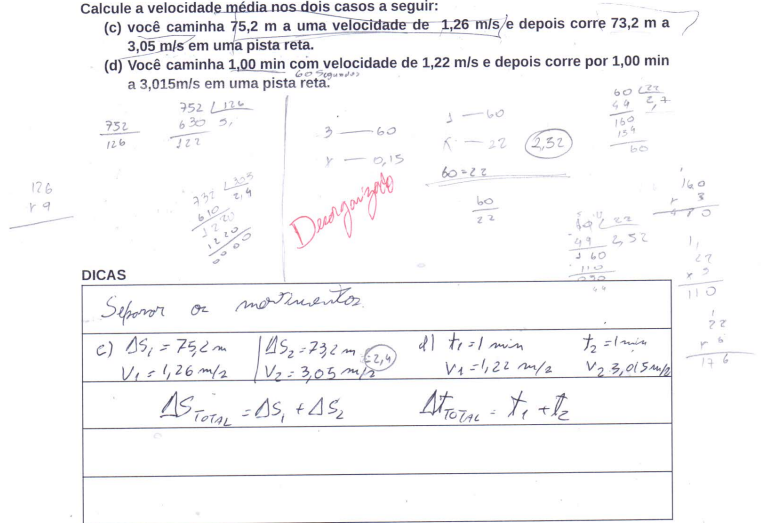
\includegraphics[width=1\textwidth]{fig/difasa1.png}
    \caption*{Fonte: Extraído da produção dos Estudantes.}
    \label{fig:difasa1}
\end{figure}

Esse cenário pode estar relacionado, também, às condições adversas causadas pela Pandemia, o que pode ter impactado negativamente a habilidade de leitura e interpretação dos enunciados pelos alunos. Essa dificuldade básica de leitura e interpretação das questões pode ter contribuído para as maiores solicitações de dicas desqualificadas durante a ASA1.

Com base na análise dos resultados da ASA1, podemos afirmar que, em relação ao objetivo \ref{item:b}, as etapas de RP que mais demandaram auxílio foram aquelas em que os alunos não conseguiam prosseguir na resolução e as que envolviam conhecimento específico de Física. Notavelmente, a falta de estudo por parte dos alunos, conforme evidenciado pelos relatos do Professor, parece estar diretamente relacionada à necessidade de auxílio nesses momentos.

Analisar a evolução temporal dos alunos na competência de Resolução de Problemas (objetivo \ref{item:c}) foi impossibilitado devido ao baixo desempenho dos mesmos. De fato, apenas alguns alunos conseguiram demonstrar um processo evolutivo representativo ao longo das atividades.

Apenas um único aluno conseguiu resolver todas as questões, sem o auxílio de dicas, o que inviabilizou a constatação de um processo evolutivo significativo. A maioria dos alunos oscilava entre os tipos de dicas solicitadas, sem obter sucesso nas resoluções, o que gerou preocupação nos pesquisadores. 

As atividades propostas eram similares às realizadas em sala de aula, indicando que os alunos não estavam estudando mesmo após o diálogo com a turma. O professor não percebeu movimentações por parte dos alunos para tirar dúvidas, tanto em aula quanto fora dela, reforçando a possível falta de empenho na busca pelo aprendizado.

Devido ao baixo desempenho dos alunos e à falta de progresso significativo durante as aplicações, não foi possível estabelecer quais formas de ajuda se tornaram mais eficientes, conforme o objetivo \ref{item:d}. Além disso, não houve oportunidades de auxiliar a turma fora das aplicações, o que dificultou ainda mais a avaliação da eficácia das dicas fornecidas. Os alunos também pareciam ter dificuldade em entender ou fazer uso das dicas. 

A última ferramenta utilizada para a análise das aplicações foi um questionário\footnote{\textbf{Pergunta 1 -} Sinto que os problemas presentes nas Atividades de Sala de Aula possuíam um grau de dificuldade similar aos problemas presentes no livro e nos realizados em sala de aula.\\ \textbf{Pergunta 2 -} Sinto que as Atividades de Sala de Aula são uma boa maneira de verificar meus conhecimentos e aprendizagens de Física.\\ \textbf{Pergunta 3 -} Sinto que as dicas presentes nas Atividades de Sala de Aula podem me auxiliar a resolver o problema quando não consigo prosseguir.\\ \textbf{Pergunta 4 -} Sinto que consigo entender melhor minhas dificuldades após a realização das Atividades de Sala de Aula.\\ \textbf{Pergunta 5 -} Considero que o número de Atividades de Sala de Aula poderia ser maior ao longo do trimestre.} (Apêndice \ref{ch:questASA}), o qual foi respondido de forma anônima e não obrigatória pelos alunos. Dos 16 alunos avaliados na ASA1, 10 deles responderam ao questionário, o que representa 62,5\% dos participantes.

\begin{table}[ht]
\centering
\caption{Respostas da ASA1 ao questionário final.} \label{tab:questASA1}
\begin{tabular}{ccccc}
\hline
\textbf{Pergunta 1} & \textbf{Pergunta 2} & \textbf{Pergunta 3} & \textbf{Pergunta 4} & \textbf{Pergunta 5} \\ \hline
5 & 4 & 5 & 3 & 4 \\ 
3 & 4 & 4 & 3 & 3 \\ 
3 & 4 & 4 & 2 & 5 \\ 
5 & 5 & 5 & 5 & 4 \\ 
4 & 5 & 5 & 5 & 5 \\ 
5 & 4 & 5 & 4 & 5 \\ 
4 & 5 & 1 & 1 & 5 \\ 
3 & 3 & 5 & 1 & 4 \\ 
4 & 3 & 1 & 1 & 5 \\ 
2 & 5 & 5 & 3 & 2 \\ \hline
\end{tabular}
\caption*{Fonte: Construção do Autor.}
\end{table}

A Tabela \ref{tab:questASA1} apresenta as respostas obtidas para as 5 perguntas, seguindo o padrão de escala Likert \cite{dalmoro}. Ao analisarmos as percepções dos alunos por meio do questionário, podemos obter uma melhor compreensão dos pontos positivos e negativos do processo até o momento. Isso nos permitirá identificar as áreas que precisam ser aprimoradas.

A primeira pergunta do questionário analisa a dificuldade das questões apresentadas na ASA. A maioria dos alunos concordou, ao menos parcialmente, que as questões eram tão difíceis quanto as apresentadas em aula. Essa concordância corrobora a informação fornecida pelo Professor de que os alunos não estavam dedicando o tempo necessário aos estudos, o que os impedia de resolver questões similares às já trabalhadas.

Os alunos também concordaram com a afirmação de que a ASA é uma boa maneira de verificar os conhecimentos de Física (pergunta 2). Eles reconhecem que, mesmo que as questões possam ser mais desafiadoras, a abordagem da ASA é uma alternativa válida em comparação com as provas tradicionais.

Quando questionados sobre a eficiência das dicas (pergunta 3), 80\% dos alunos que responderam concordaram que elas foram úteis. Entretanto, os outros 20\% discordaram totalmente da afirmação. É importante considerar que alguns alunos podem ter enfrentado dificuldades externas ao conteúdo de Física, o que pode ter impactado a percepção sobre a eficácia das dicas. Diante disso, é necessário repensar as estratégias das dicas para que mais alunos se sintam confortáveis ao fazer uso delas.

Uma observação importante, embora não surpreendente, é que a maioria dos alunos relatou não conseguir compreender melhor suas dificuldades após as aplicações da ASA (pergunta 4). Isso pode estar diretamente relacionado ao fato de que, nesta turma específica, os alunos enfrentaram dificuldades em fazer uso efetivo das dicas fornecidas durante o processo.

Observamos ainda que, em muitos casos, os alunos tinham receio de solicitar ajuda devido à redução no valor máximo da atividade. No entanto, parece que eles não percebiam que, caso não conseguissem resolver a questão, seu resultado seria ainda pior. Essa hesitação pode ter contribuído para a menor utilização das dicas e, consequentemente, para o menor progresso nas resoluções das questões.

Surpreendentemente, 80\% dos alunos responderam que poderiam ser realizadas mais aplicações da ASA ao longo do período letivo (pergunta 5). É importante considerar que o número de intervenções já foi elevado, uma vez que foram realizadas 3 aplicações ao invés de uma única prova. A opinião dos alunos sugere que eles perceberam os benefícios das aplicações e se sentiram mais confortáveis com esse formato de avaliação.

As respostas dos alunos nas observações e reclamações acerca do modelo das ASA (pergunta dissertativa) mostraram-se limitadas, uma vez que alguns alunos não pareceram compreender totalmente a proposta da pergunta. Alguns dos participantes deixaram esse espaço em branco, o que pode indicar falta de clareza sobre como abordar o assunto ou simplesmente a ausência de reclamações significativas. 

As respostas, em sua maioria, foram relacionadas às aulas do Professor, e não às atividades em si. As reclamações estavam relacionadas ao tempo dedicado pelo Professor em sala de aula para a explicação de cada tópico do conteúdo. Em resposta a essas preocupações, houve um diálogo com a turma, onde o Professor explicou que o conteúdo a ser trabalhado é muito extenso para a quantidade de períodos letivos semanais, o que limita o tempo disponível para aprofundar cada tópico.

Foi reforçada a importância dos estudantes dedicarem tempo ao estudo em casa e enviarem suas dúvidas para o Professor. Esse processo de comunicação e apoio fora das aulas presenciais foi enfatizado desde o início do ano letivo como uma forma de proporcionar um melhor aproveitamento do conteúdo e esclarecer as dificuldades enfrentadas pelos alunos. 

Com base nas informações obtidas pelo questionário e nas anotações e observações do Professor, não foi possível identificar uma manutenção do interesse na resolução de problemas ao longo do trimestre (objetivo \ref{item:e}). De fato, podemos afirmar que, de modo geral, essa turma não demonstrou interesse em buscar meios para desenvolver suas habilidades nessa área. O fato de não buscarem ajuda, tanto em sala de aula quanto fora dela, e a falta de evolução significativa na resolução dos problemas sugerem uma falta de engajamento e motivação por parte dos alunos em aprimorar sua competência de resolução de problemas de Física.

\subsection{ASA2} \label{subsec:asa2}


A ASA2 contou com a participação de 21 alunos, de um total de 26 matriculados na turma de 2º ano do Ensino Médio (ver Tabela \ref{tab:basicoASA}). Os critérios para escolha da turma e exclusão de determinados alunos foram os mesmos utilizados na ASA1.

O Professor já havia ministrado a disciplina de Física para essa turma no 1º ano do Ensino Médio. Antes disso, os estudantes passaram pelo 8º ano do Ensino Fundamental em formato remoto, devido à Pandemia, e pelo 9º ano de forma híbrida.

Da mesma forma que ocorreu na turma da ASA1, houve uma flexibilização das faltas na escola quando o Professor lecionou pela primeira vez para a turma. Isso ocorreu devido às dificuldades de adaptação dos alunos no retorno ao sistema presencial, e alguns deles estavam em risco de abandonar os estudos.

A flexibilização das faltas foi essencial para evitar a evasão escolar. No entanto, durante o processo de aplicação da ASA2, ainda foram percebidos resquícios da dificuldade de adaptação por parte de alguns estudantes. Essa situação resultou em defasagens nos conhecimentos dos alunos, impactando o desenvolvimento das atividades.

Durante o 1º ano, o Professor assumiu a turma na metade do ano letivo e constatou que o conteúdo programático estava atrasado. Como resultado, não foi possível abranger todo o conteúdo previsto para o 1º ano do Ensino Médio. Essa lacuna na formação dos estudantes tem impacto direto ao gerar dificuldades adicionais no processo de aprendizagem dos estudantes.

Durante a ASA2, considerando as dificuldades pré-existentes dos alunos com operações matemáticas e interpretação de texto, era esperado observar uma maior quantidade de solicitações de dicas desqualificadas e de Matemática. Esses aspectos poderiam impactar diretamente o desempenho dos estudantes nas atividades propostas, uma vez que essas habilidades são fundamentais para a RP de Física. 

\begin{figure}[ht]
\begin{center}
\caption{Gráfico das dicas solicitadas ao longo da ASA2.}
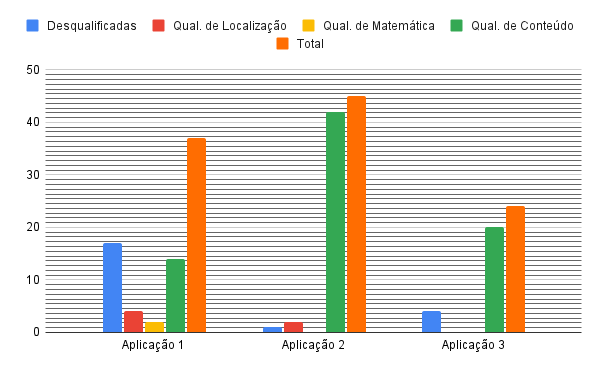
\includegraphics[width=1\textwidth]{fig/graficoDicasASA2.png}
\label{fig:dicasASA2}
\caption*{Fonte: Construção do Autor.}
\end{center}
\end{figure}

Ao longo da ASA2, foram conduzidas 3 aplicações que estão disponíveis no Apêndice \ref{apendice:asa2}. A Figura \ref{fig:dicasASA2} apresenta um gráfico ilustrando a quantidade e o tipo de dicas fornecidas aos alunos durante cada uma dessas três atividades. Essas informações são relevantes para entendermos o auxílio que os estudantes buscaram ao enfrentar os problemas propostos e para analisar os padrões de dificuldades encontrados pelos alunos.

A aplicação 1 (Apêndice \ref{ch:ASA2a1}) consistia em um problema de conversão de escalas térmicas. Durante as aulas expositivas, o Professor ensinou os alunos a realizar a conversão entre as três escalas térmicas mais comuns - Celsius, Kelvin e Fahrenheit. Além disso, foi demonstrado como criar uma equação geral de conversão entre duas escalas de temperatura quaisquer, proporcionando aos estudantes ferramentas para resolver problemas envolvendo esse tipo de conversão.

Esperávamos que os alunos não encontrassem dificuldades significativas no processo de resolução da aplicação 1. No entanto, caso solicitassem dicas, esperávamos que fossem do tipo qualificadas, possivelmente relacionadas a Matemática ou ao Conteúdo (específico da conversão de escalas térmicas). A expectativa das dicas de Matemática decorria do histórico de dificuldades da turma nessa área, enquanto as de Conteúdo poderiam surgir caso os alunos não se lembrassem de algum detalhe relevante para realizar a conversão.

Ao analisarmos a Figura \ref{fig:dicasASA2}, percebemos que nossas expectativas em relação às dicas de Conteúdo se confirmaram. No entanto, ao invés de termos um número elevado de estudantes com dificuldades em Matemática, a maioria deles enfrentou dificuldades no início da resolução do problema, o que resultou na solicitação de dicas desqualificadas. 

Isso indica que a turma enfrentou obstáculos no início do processo de resolução, possivelmente relacionados à compreensão do enunciado ou à identificação dos dados relevantes para a conversão de escalas térmicas. Esses obstáculos revelam que a dificuldade previamente mencionada em interpretação de texto dos estudantes pode ser mais desafiadora do que inicialmente esperado.

Dos 21 alunos avaliados, 5 não solicitaram nenhuma dica durante a aplicação 1. Dentre esses, 2 conseguiram resolver a questão. Um deles já era esperado, sendo reconhecido como um bom aluno e participante assíduo de provas e olimpíadas estudantis, frequentemente recebendo premiações.

O outro estudante que acertou a questão foi um dos que quase abandonou a escola. Ele relatou ao Professor que havia começado a estudar e se dedicaria a isso. Esses casos se repetirão ao longo da ASA2, tornando relevante a antecipação dessa informação para evitar repetições posteriores.

O processo da aplicação 2 (Apêndice \ref{ch:ASA2a2}) abordou os conceitos de transferência de calor e mudança de estado físico. Em sala de aula, o Professor já havia resolvido questões semelhantes com os alunos, mas a principal diferença nesta aplicação foi a necessidade de realizar duas mudanças de estado físico, em contraste com as questões abordadas anteriormente, que envolviam apenas uma mudança.

Essa diferença foi estabelecida com o propósito de transformar o que seria um simples exercício, uma vez que os alunos já estavam familiarizados com a resolução, em um desafio que exigiria a aplicação de conhecimentos prévios. Nesse contexto, esperávamos que, de maneira geral, a turma não precisasse de muitas dicas, com exceção talvez da parte Matemática, em virtude das características prévias dos alunos, e da parte de Conteúdo, devido às diferenças em relação ao que já haviam aprendido anteriormente.

A análise dos tipos de dicas utilizados confirmou nossas previsões. A grande maioria das dicas solicitadas pelos alunos foram de Conteúdo. Especificamente, as perguntas mais frequentes referiam-se às equações do calor sensível, do calor latente e como calcular o calor total no processo.

Isso indica que, apesar dos alunos não terem memorizado as equações, eles tinham conhecimento do procedimento necessário para resolver o problema, e as dicas foram úteis nesse processo. Infelizmente, a maioria dos alunos não conseguiu concluir a resolução corretamente ou resolveu de forma equivocada.

Nesses casos, os alunos acabaram cometendo erros em operações básicas matemáticas ou não conseguiram responder corretamente à pergunta. Isso evidencia novamente a dificuldade dos alunos na interpretação de texto e na execução de operações matemáticas. Essas habilidades são fundamentais para a resolução adequada de problemas, e a identificação dessas dificuldades destaca a necessidade de focar no desenvolvimento dessas competências ao longo do processo educacional.

A identificação de 5 alunos que não pediram dicas durante a aplicação 2, sendo que 3 deles erraram a questão, é um indicativo importante sobre o engajamento e a disponibilidade desses estudantes para dedicarem-se aos estudos de Física. O fato de estarem participando de aulas no contra turno e outras atividades extracurriculares pode estar impactando negativamente o tempo disponível para o estudo individual, prejudicando assim o seu desempenho nas atividades propostas.

Durante o processo da aplicação 3 (Apêndice \ref{ch:ASA2a3}), trabalhamos novamente a transferência de calor, mas dessa vez, utilizando mais conceitos da termometria em comparação à atividade anterior. Essencialmente, abordamos os mesmos fenômenos físicos, porém com enfoques distintos.

Ao analisar a Figura \ref{fig:dicasASA2}, observamos uma redução significativa no número total de dicas solicitadas em relação às duas outras aplicações. Além disso, notamos que essas dicas foram, em sua maioria, do tipo Conteúdo.

A redução no número total de dicas se deve, possivelmente, ao fato de termos mais alunos que não solicitaram dica nenhuma, totalizando 8. Além disso, as dicas de Conteúdo mostram que os alunos não se preocuparam em memorizar as equações, já que poderiam solicitar ajuda, mas mantiveram o foco em entender os procedimentos para saber como aplicar as dicas.

Outra observação positiva que podemos fazer acerca desta aplicação é o fato de mais estudantes terem conseguido completar a resolução. Infelizmente, nem todos acertaram completamente, apresentando erros matemáticos ou alguma falha procedimental. No entanto, eles se esforçaram para fazer o máximo possível, onde mais de 60\% da turma não abandonou o processo de resolução.

O empenho e a dedicação dos alunos em permanecer no processo de resolução de problemas refletem uma atitude positiva. Essa perseverança evidencia um interesse genuíno em aprimorar suas habilidades de RP e a disposição para enfrentar os desafios que surgem durante o processo.

A atitude dos alunos em não desistir diante de erros e falhas é positiva e motivadora, demonstrando engajamento no processo de aprendizado e disposição para enfrentar os desafios da RP de Física. Essa postura é essencial para o desenvolvimento das habilidades na RP e para o progresso dos estudantes no contexto educacional.

\begin{table}[ht]
\centering
\caption{Principais perguntas dos alunos durante a ASA2.} \label{tab:pergASA2}
\begin{tabular}{c|c}
\hline
\textbf{Perguntas} & \textbf{Classificação}\\ \hline
O que eu faço com essas duas escalas? & Desqualificada \\
Preciso utilizar os valores do enunciado para resolver a questão? & Desqualificada \\
Pode me ajudar a montar o diagrama de fases? & Conteúdo \\
Qual o modelo da equação de conversão? & Conteúdo \\
Quais são as equações do calor? & Conteúdo\\
\hline
\end{tabular}
\caption*{Fonte: Construção do Autor.}
\end{table}

Na Tabela \ref{tab:pergASA2} trazemos algumas das perguntas que mais foram realizadas pelos estudantes ao longo do processo da ASA2. Nela também vemos a classificação dessas perguntas, em acordo com os critérios adotados para a classificação das respostas.

\subsubsection{Considerações Gerais da ASA2} \label{subsubsec:asa2}

Nesta etapa, conduziremos uma análise geral da ASA2, abordando aspectos das três aplicações. Para tal, utilizaremos as ferramentas de pesquisa descritas na Seção \ref{sec:asa}, conectando-as aos objetivos deste estudo.

A primeira ferramenta de análise que abordaremos são as folhas de resposta dos alunos. Nossa expectativa era encontrar as questões resolvidas de forma ordenada e organizada, além de observar o uso de desenhos e diagramas durante o processo de resolução. Essa ferramenta está conectada ao objetivo \ref{item:a}, que visa compreender como os alunos abordam a RP de Física.

Compreendemos que essa expectativa se baseia no conhecimento prévio sobre as condições da turma, considerando que eles já tiveram experiência prévia com a disciplina de Física. Apesar das lacunas de conhecimento existentes, os alunos demonstram esforço na busca por melhorar seus resultados e habilidades de RP.

Ao analisarmos as folhas de resposta, constatamos que a maioria dos estudantes confirmou nossas expectativas. Embora alguns precisassem de ajuda para lembrar como iniciar o processo de resolução de problemas, ao resolverem a questão, seguiam sempre uma estrutura lógica consistente.

A estrutura lógica observada consistia em três etapas principais: identificação e anotação das informações e objetivos da questão, criação de um esboço ou diagrama do processo envolvido, e posteriormente, traçar e implementar uma estratégia para a resolução. Essa abordagem se assemelha ao processo descrito por \citeonline{Pozo2009}, o que indica uma similaridade na forma de abordar e resolver problemas de Física entre os alunos da ASA2 e os estudantes da ASA1.

Ao longo das três aplicações, a turma utilizou um total de 106 dicas. Dentre essas, 22 foram consideradas desqualificadas, 6 de Localização, apenas 2 de Matemática e 76 de Conteúdo. As dicas desqualificadas tiveram como objetivo lembrar os alunos de analisar as informações presentes no problema e reforçar a possibilidade de criar diagramas para auxiliar na interpretação e resolução dos problemas.

Constatamos que, ao contrário do que inicialmente imaginávamos, os alunos não solicitaram muitas dicas de Matemática durante as aplicações. No entanto, durante a análise do processo, observamos que as dificuldades em matemática básica ainda persistem entre os estudantes (Figura \ref{fig:mtmasa2}). Afinal, foram identificados erros em operações simples, como multiplicação de números inteiros. 

\begin{figure}[ht]
\begin{center}
\caption{Exemplo de dificuldade em Matemática ao longo da ASA2.}
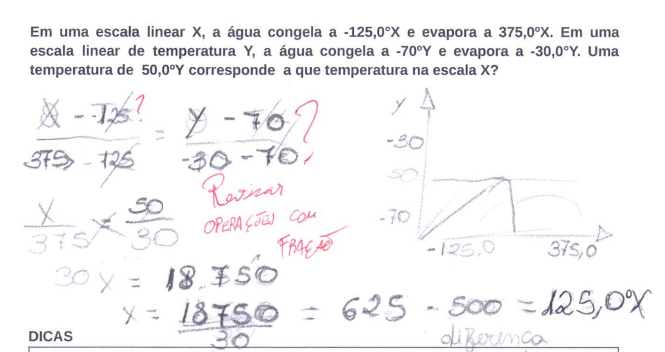
\includegraphics[width=1\textwidth]{fig/mtmasa2.png}
\label{fig:mtmasa2}
\caption*{Fonte: Extraído da produção dos Estudantes.}
\end{center}
\end{figure}


Nesse contexto, emerge a hipótese de que os alunos possam não estar suficientemente atentos durante o processo de resolução. Além disso, aqueles que enfrentaram dificuldades e não avançaram significativamente na resolução podem não ter solicitado dicas de Matemática por não terem alcançado uma etapa em que essa forma de auxílio fosse necessária.

No que diz respeito às dicas de Conteúdo, que foram a maioria nesta aplicação, é importante analisar o contexto geral em que foram solicitadas. Os alunos, após conseguirem estruturar o processo de resolução, enfrentavam dificuldades em recordar as equações necessárias. Nessas situações, eles faziam questionamentos direcionados, solicitando, por exemplo, uma equação pelo nome da variável que buscavam. 

De fato, os alunos demonstraram um bom discernimento sobre o que procurar para progredir na resolução da questão. É provável que, nessas situações, se houvesse um formulário na atividade com as informações relevantes, eles não teriam necessitado solicitar essa dica específica, pois teriam acesso direto às informações necessárias para avançar na resolução - como mostrado na Figura \ref{fig:dicasasa2}. Isso evidencia, novamente, que os estudantes estavam mais focados em compreender o processo de resolução e em como aplicar as dicas de Conteúdo de forma adequada, em vez de depender apenas da memorização das equações.

\begin{figure}[ht]
\begin{center}
\caption{Exemplo de Dicas fornecidas ao longo da ASA2.}
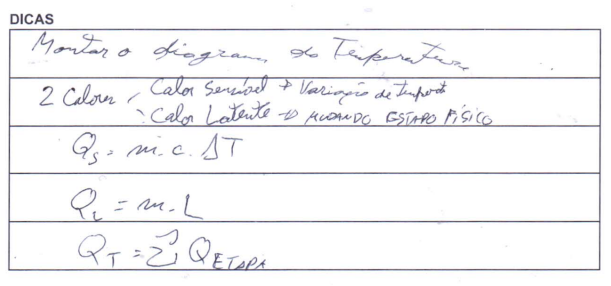
\includegraphics[width=1\textwidth]{fig/dicasasa2.png}
\label{fig:dicasasa2}
\caption*{Fonte: Extraído da produção dos Estudantes.}
\end{center}
\end{figure}

Concluindo, constatamos que, em relação ao objetivo \ref{item:b}, a etapa que mais demandou auxílio durante o processo de Resolução de Problemas foi a de Conteúdo, seguida da etapa inicial em que as dicas desqualificadas guiaram o processo. No entanto, é igualmente importante observar as dicas de Matemática, que também possuem potencial de serem mais solicitadas, mediante avanço no processo resolutivo.

Durante o processo da ASA2, pudemos observar uma evolução no processo de Resolução de Problemas (objetivo \ref{item:c}) por parte dos alunos. Ao analisarmos a Figura \ref{fig:dicasASA2}, percebemos uma oscilação na quantidade total de dicas utilizadas ao longo das aplicações.

Durante o período entre a aplicação 1 e a aplicação 2, observamos um aumento significativo no número total de dicas utilizadas pelos alunos. Esse aumento se refletiu, principalmente, na conversão de dicas desqualificadas para dicas de Conteúdo. Ou seja, os alunos passaram a solicitar menos dicas de caráter genérico e mais dicas específicas relacionadas ao conteúdo das questões.

Essa mudança indica um progresso na capacidade dos alunos de compreender e aplicar os processos envolvidos na RP. Ao se depararem com desafios mais complexos, eles demonstraram uma maior habilidade em identificar quais informações eram necessárias para prosseguir e quais conceitos precisavam ser aplicados para chegar à solução.

A redução significativa no número total de dicas utilizadas entre a aplicação 2 e a aplicação 3 reflete o aprimoramento das habilidades dos alunos em RP. Eles se tornaram mais conscientes do processo de RP e demonstraram uma maior autonomia na resolução das questões, necessitando de menos auxílio ao longo do caminho.

O estilo de dicas utilizado pelos alunos se manteve consistente, com uma ênfase maior em solicitar dicas de Conteúdo, o que indica que eles estavam buscando compreender e aplicar os conceitos específicos das questões.

Essa evolução positiva na resolução dos problemas mostra que os alunos assimilaram os conceitos trabalhados durante as atividades anteriores e adquiriram uma maior compreensão das estratégias para solucionar as questões propostas. Ao colocar em prática o que aprenderam, eles demonstraram um melhor domínio das habilidades de RP, o que contribuiu para o êxito alcançado na aplicação 3.

Através das observações feitas pelos alunos durante os processos de aplicação, percebemos uma preferência clara em relação ao formato das dicas (objetivo \ref{item:d}). Essa conclusão foi obtida após os alunos relatarem que certas explicações não foram compreendidas no momento em que as dicas foram fornecidas.

Durante as aplicações, ao fornecer dicas desqualificadas, observamos que os alunos demonstravam preferir um estilo em que lhes fossem apresentados apontamentos sobre como prosseguir. Por exemplo, na aplicação 1 (Apêndice \ref{ch:ASA2a1}), os estudantes pareceram entender melhor a informação quando lhes era dito: "Você sabe que existem 2 escalas de Temperatura e precisa relacioná-las. Como fazer isso?"

Ao receber essa informação, os alunos eram levados a refletir sobre o assunto. Na maioria dos casos, esse tipo simples de dica, seguida de um questionamento, levava os estudantes a progredir. Esse progresso ocorria de duas formas: através da resolução do problema ou da formulação de uma nova pergunta, geralmente de forma Qualificada.

Além das dicas desqualificadas, vamos abordar a eficiência das dicas de Conteúdo, uma vez que constituíram a maior parte das orientações fornecidas. Nesse contexto, identificamos duas formas distintas de Conteúdo: teoria e prática.

As dicas de teoria abordavam conceitos fundamentais e equações relacionadas ao problema, enquanto as dicas de prática forneciam orientações mais diretas sobre como aplicar esses conceitos na resolução específica da questão.

Quando a dúvida dos alunos estava relacionada à lembrança de uma equação, foi mais eficiente e útil fornecer-lhes diretamente a equação necessária. Dessa forma, eles puderam aplicar as informações que já haviam extraído e prosseguir com mais facilidade em seu desenvolvimento no processo de resolução.

Quando a dúvida dos alunos estava relacionada aos conceitos da matéria, foi necessário fornecer uma pequena explicação sobre aquela parte específica do conteúdo. Por exemplo, na aplicação 2 (Apêndice \ref{ch:ASA2a2}), os alunos precisavam calcular o calor total em um processo de mudança de fase. Muitos deles apresentaram dúvidas sobre como aplicar os calores sensível e latente nessa situação.

Nesse contexto, a dica foi fornecida na forma de uma explicação rápida, como "O calor sensível será utilizado quando houver mudança de estado físico." Essa abordagem permitiu que os alunos compreendessem como utilizar os conceitos de calor sensível e latente na resolução do problema específico e avançassem em sua resolução com maior clareza e segurança.

\begin{table}[H]
    \centering
    \caption{Respostas da ASA2 ao questionário final.}\label{tab:questASA2}
    \begin{tabular}{ccccc}
    \hline
        \textbf{Pergunta 1} & \textbf{Pergunta 2} & \textbf{Pergunta 3} &\textbf{Pergunta 4} & \textbf{Pergunta 5} \\ \hline
        1 & 1 & 2 & 1 & 1 \\ 
        1 & 4 & 4 & 4 & 1 \\ 
        2 & 5 & 5 & 2 & 1 \\ 
        1 & 4 & 5 & 4 & 2 \\ 
        3 & 1 & 2 & 1 & 1 \\ 
        1 & 1 & 2 & 1 & 1 \\ 
        1 & 4 & 4 & 4 & 1 \\ 
        2 & 1 & 1 & 1 & 1 \\ 
        1 & 2 & 2 & 1 & 2 \\ 
        2 & 3 & 4 & 3 & 2 \\ 
        3 & 4 & 5 & 2 & 4 \\ 
        3 & 4 & 5 & 3 & 1 \\ 
        3 & 5 & 5 & 3 & 3 \\ 
        2 & 4 & 2 & 3 & 2 \\ 
        1 & 1 & 1 & 1 & 1 \\ 
        2 & 4 & 3 & 4 & 3 \\ 
        3 & 2 & 5 & 4 & 5 \\ 
        3 & 1 & 4 & 1 & 3 \\ 
        1 & 5 & 3 & 5 & 5 \\ 
        3 & 1 & 2 & 4 & 2 \\ \hline
    \end{tabular}
    \caption*{Fonte: Construção do Autor.}
\end{table}

A Tabela \ref{tab:questASA2} apresenta os resultados obtidos para as cinco primeiras perguntas do questionário (Apêndice \ref{ch:questASA}) aplicado ao fim da ASA2. Assim como realizado para a ASA1, procederemos com a análise e discussão das respostas para cada pergunta de forma individual.

O alto índice de participação dos alunos no questionário da ASA2, com 20 dos 21 alunos avaliados respondendo, é um fator positivo a ser destacado. Isso reforça o perfil engajado da turma, demonstrando que os estudantes estão interessados em contribuir com a avaliação do processo de RP e em compartilhar suas percepções sobre as atividades desenvolvidas.

Essa atitude pró-ativa dos alunos em participar do questionário mostra que eles estão dispostos a fornecer \textit{feedbacks} relevantes para o aprimoramento do processo de ensino-aprendizagem. Além disso, ao expressarem suas opiniões e experiências, os alunos podem contribuir para que o professor compreenda melhor suas necessidades e dificuldades, auxiliando na identificação de pontos fortes e áreas de melhoria nas próximas aplicações da ASA ou em outras atividades pedagógicas.

Diferentemente das respostas obtidas na ASA1, aqui tivemos discordância quanto ao grau de dificuldade das questões durante as aplicações (pergunta 1). Ao compararmos as questões antes e depois da modificação para uso na ASA, conforme exemplificado na Tabela \ref{ref:questoes} na Seção \ref{sec:asa}, podemos inferir que os alunos podem não ter se familiarizado plenamente com o estilo de modificações nas questões durante a ASA2. Essa falta de familiaridade pode ter influenciado na percepção de dificuldade, levando a uma divergência nas respostas.

Houve uma divisão de opiniões na turma quanto à eficácia da ASA em avaliar os conhecimentos e aprendizagens de Física (pergunta 2). É importante lembrar que a ASA é uma abordagem diferenciada de avaliação, que visa estimular o desenvolvimento das habilidades de RP, indo além da simples memorização de conteúdos.

Os alunos que manifestaram dificuldades ou preferência por outro modelo de avaliação podem estar acostumados a formatos mais tradicionais, onde a ênfase é na memorização de fórmulas e conceitos, e a resolução de exercícios se assemelha a repetir fórmulas prontas. A ASA, por outro lado, busca incentivar a autonomia dos alunos, a capacidade de enfrentar desafios e a aplicação prática do conhecimento adquirido.

A divergência de opiniões dos alunos em relação à qualidade das dicas apresentadas na ASA é uma reflexão importante para aprimorar o processo (pergunta 3). O fato de alguns alunos não se sentirem confiantes ou convencidos da eficácia das dicas pode ter influenciado na utilização das mesmas ao longo da ASA.

Para melhorar a aceitação e efetividade das dicas, é necessário buscar alternativas que possam atender às diferentes necessidades dos alunos. Isso pode envolver a oferta de diferentes tipos de dicas, como exemplos detalhados, explicações mais aprofundadas ou até mesmo recursos visuais e práticos para auxiliar na compreensão dos conceitos.

A análise das respostas da pergunta 4 do questionário, que abordou a sensação de compreensão das próprias dificuldades após as aplicações da ASA, evidenciou, novamente, uma divisão de opiniões na turma. Os alunos que não demonstram confiança no processo das dicas provavelmente não experimentaram uma mudança significativa em sua percepção sobre suas próprias dificuldades na disciplina.

Essa divergência pode estar diretamente relacionada à eficácia percebida das dicas oferecidas durante as aplicações. Os estudantes que não se sentem confiantes na utilidade ou eficácia das dicas podem não ter vivenciado uma melhora substancial em sua compreensão das dificuldades enfrentadas no aprendizado da Física.

Essa constatação ressalta a importância de revisar e aprimorar o processo de fornecimento de dicas, visando torná-las mais efetivas e relevantes para atender às necessidades individuais dos alunos. Além disso, é fundamental considerar outros fatores que podem influenciar a percepção dos alunos sobre suas dificuldades, como a abordagem do conteúdo em sala de aula, o ambiente de aprendizagem e a motivação dos estudantes.

A análise da pergunta 5 do questionário evidencia que a maioria dos alunos discorda da possibilidade de mais aplicações ao longo do trimestre. Essa preferência é fundamentada na percepção de que eles valorizam mais as atividades realizadas em sala de aula e as aulas expositivas. A limitação de tempo durante as aulas, devido à realização das aplicações, pode ser um fator que contribui para essa preferência, uma vez que os estudantes desejam mais oportunidades de interação com o professor e atividades tradicionais em sala de aula para fortalecer o aprendizado. 

Ao analisar o interesse na Resolução de Problemas (RP) ao longo do trimestre (objetivo \ref{item:e}), podemos afirmar que houve, de fato, interesse por parte dos alunos. Apesar de discordarem dos meios utilizados, ou seja, das aplicações, todos os alunos fizeram o esforço de buscar resolver as questões apresentadas da melhor forma possível. Esse comportamento evidencia que eles se empenharam em enfrentar os desafios propostos e demonstraram interesse em desenvolver suas habilidades de RP, mesmo que as estratégias de avaliação não tenham sido totalmente satisfatórias para eles. Portanto, o interesse dos alunos pela RP se manteve presente ao longo do trimestre, mesmo com as discordâncias sobre as formas de avaliação.


\subsection{ASA3} \label{subsec:asa3}

A seleção da turma do 3º ano do Ensino Médio para esta etapa do estudo foi definida pelo fato de o autor deste trabalho ser o professor regente da turma. Além disso, o professor já havia lecionado para essa mesma turma no ano anterior, o que permitiu uma familiaridade maior com as características e o histórico de aprendizado dos alunos.

Com base na experiência anterior do professor com a turma do 3º ano do Ensino Médio e nas condições de ensino que os alunos enfrentaram no 1º ano do Ensino Médio (formato híbrido) e no 9º ano do Ensino Fundamental (formato remoto), sabíamos que eles poderiam apresentar dificuldades prévias em Matemática e Física. Essas dificuldades poderiam ser semelhantes às observadas na turma da ASA2, considerando a transição entre o Ensino Fundamental e o Ensino Médio e as adaptações ao ensino remoto e híbrido.

Durante a experiência de lecionar para a turma do 2º ano do Ensino Médio, o professor observou que existem dificuldades notórias em Matemática e Física. No entanto, ele também destaca que essa turma se destaca pelo empenho e dedicação aos estudos. Essa característica positiva dos alunos pode ser um fator motivador para enfrentar os desafios encontrados na disciplina e buscar melhorar suas habilidades de RP.

Com base nas características positivas observadas da turma durante o 2º ano do Ensino Médio, como o empenho e dedicação aos estudos, as expectativas em relação ao rendimento da turma durante a ASA3 são bastante otimistas. Acreditamos que os alunos possuirão uma postura ativa e comprometida no processo de RP em Física, buscando superar desafios e aprimorar suas habilidades.

Além disso, esperamos que os estudantes forneçam boas observações e \textit{feedbacks} sobre a experiência com a ASA3. A turma já possui uma relação de confiança com o professor, o que pode favorecer a abertura para expressar suas opiniões de forma construtiva. Essas observações serão valiosas para avaliar a efetividade das estratégias pedagógicas adotadas e para identificar possíveis melhorias no processo de resolução de problemas.

\begin{figure}[ht]
\begin{center}
\caption{Gráfico das dicas solicitadas ao longo da ASA3.}
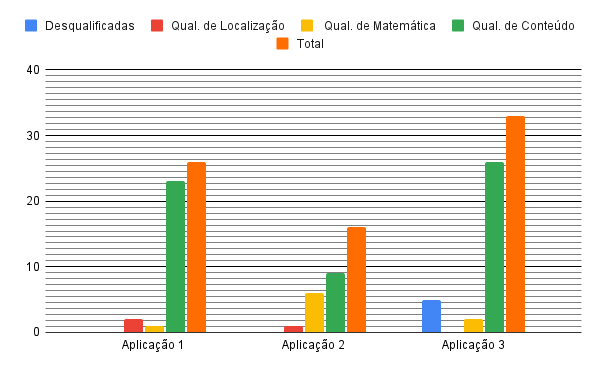
\includegraphics[width=1\textwidth]{fig/graficoDicasASA3.png}
\label{fig:dicasASA3}
\caption*{Fonte: Construção do Autor.}
\end{center}
\end{figure}

A turma do 3º ano do Ensino Médio, composta por 19 alunos, teve a participação de 14 estudantes avaliados durante o processo da ASA3. A exclusão de alguns alunos do estudo ocorreu pelos mesmos motivos já citados anteriormente, como questões de saúde, ausência na data da aplicação das atividades ou outros impedimentos que inviabilizaram a participação na ASA3.

A Figura \ref{fig:dicasASA3} apresenta a quantidade e o tipo de dicas fornecidas ao longo do processo da ASA3. É notável que há uma variação significativa no número total de dicas fornecidas em cada aplicação, o que nos leva a uma análise detalhada das razões por trás dessas oscilações.

Durante a aplicação 1 (Apêndice \ref{ch:ASA3a1}), foi trabalhada uma questão sobre carga elétrica. Nessa atividade, os alunos foram desafiados a calcular a quantidade de elétrons que deveriam ser retirados ou adicionados a um corpo para que ele assumisse uma carga elétrica específica.

Antes do início do processo das aplicações da ASA3, a turma foi informada sobre a necessidade de saber utilizar corretamente as sub e supra unidades de medida. Essa informação gerou preocupação entre os estudantes, que relataram ter dificuldades em memorizar esse tipo de informação. 

A decisão de enfatizar o uso correto das sub e supra unidades de medida foi motivada pelo entendimento de que a turma enfrentaria desafios em avaliações futuras, como Vestibulares e ENEM, onde informações específicas sobre essas unidades nem sempre são fornecidas. Além disso, é importante considerar que os níveis de exigência das questões podem variar ao longo do Ensino Médio.

Com base nas preocupações manifestadas pelos alunos, esperávamos observar um grande número de solicitações de dicas de Conteúdo, especialmente relacionadas às sub e supra unidades de medida. Ao contrário das aplicações anteriores, não tínhamos tanta expectativa em relação a solicitações de dicas de Matemática, já que os alunos não demonstraram preocupações específicas nessa área.

Analisando a Figura \ref{fig:dicasASA3}, podemos observar que houve apenas 1 solicitação de dica de Matemática. No entanto, contrariando nossas expectativas, os alunos demonstraram mais dificuldades na utilização dos conceitos matemáticos do que a quantidade de solicitações de dicas sugere. 

Essa discrepância pode ser um indicativo de que os alunos enfrentaram dificuldades matemáticas, mas talvez tenham relutado em pedir ajuda nessa área específica durante o processo de resolução das questões, ou, pior ainda, não tenham percebido que suas operações estavam equivocadas.

Dos alunos avaliados, 3 não solicitaram nenhuma dica. Observamos que esses alunos apresentaram dificuldades nos conceitos matemáticos, especificamente na inabilidade de operar com potências. Parece que eles preferiram não pedir ajuda durante o processo de resolução. Após a correção da atividade, o professor sugeriu que revisassem esse conteúdo, pois é fundamental para o desenvolvimento ao longo do ano letivo.

Nossa expectativa sobre as dúvidas de Conteúdo foi confirmada. Além de serem a maioria das dicas fornecidas, quase em sua totalidade as dicas de Conteúdo serviram para responder à pergunta: "Quanto vale um micro Coulomb?". Esse resultado evidencia a dificuldade dos alunos em memorizar e utilizar as subunidades

A questão da aplicação 2 (Apêndice \ref{ch:ASA3a2}) aborda o cálculo da força elétrica entre partículas e apresenta uma situação interessante, pois os alunos já haviam resolvido uma questão semelhante em sala de aula, envolvendo duas partículas. Nesta aplicação, há uma terceira partícula que deve ser colocada de forma a manter o equilíbrio das forças.

Isso nos permite avaliar não apenas os conhecimentos sobre eletricidade relacionados ao conteúdo, mas também revisitar noções vetoriais que devem ter sido trabalhadas ao longo do 1º ano do Ensino Médio. Essa abordagem ampla da questão proporciona aos alunos uma oportunidade de aplicar conceitos aprendidos anteriormente em um contexto mais complexo e desafiador.

Na aplicação 2, observamos o menor número de dicas solicitadas em comparação com todas as outras da ASA3. Além disso, também foi a aplicação em que o maior número de alunos, 4 no total, optou por não solicitar nenhuma dica.

A observação de que a redução no número de dicas solicitadas na aplicação 2 não resultou em uma melhoria no desempenho médio da turma é um indicativo relevante. Isso pode sugerir que os alunos não tenham compreendido completamente a proposta das atividades ou que não tenham consolidado seus conhecimentos de forma significativa.

Por possuir uma boa relação com a turma, o Professor questionou-os sobre os motivos de não estarem solicitando tantas dicas quanto, aparentemente, necessitavam. A resposta obtida foi que eles estariam se testando, visto que possuem preocupações com relação ao futuro e aprovações em provas para ingresso na faculdade.

O Professor demonstrou compreensão e empatia em relação às preocupações dos alunos e tranquilizou-os, explicando que as atividades da ASA tem exatamente o propósito de analisar o nível de ajuda que eles necessitam. Além disso, ressaltou que essas informações serão utilizadas para auxiliá-los no aprimoramento de suas habilidades de resolução de problemas durante as aulas.

Essa abordagem do Professor é muito importante, pois mostra aos alunos que as atividades não são apenas uma forma de avaliação, mas sim uma ferramenta para identificar suas dificuldades e pontos a serem aprimorados. Ao utilizar os resultados das atividades para planejar o conteúdo das aulas e direcionar a abordagem dos temas em sala, o Professor pode contribuir significativamente para o desenvolvimento dos alunos.

Após a conversa com o Professor, houve a aplicação 3, que abordou o conceito de força elétrica exercida por um campo (Apêndice \ref{ch:ASA3a3}). Considerando as impressões deixadas pela turma após a conversa, era esperado um aumento no número de dicas solicitadas. No entanto, não tínhamos clareza sobre qual tipo específico de dica seria mais solicitado pelos alunos.

A previsão de aumento na solicitação de dicas se confirmou, e, de fato, foi a maior de toda a ASA3. Seguindo esse padrão, essa foi a atividade em que menos alunos deixaram de pedir dicas, sendo apenas 1 estudante que não solicitou dicas durante a atividade e acabou errando.

O diálogo com a turma mostrou-se efetivo. Eles passaram a compreender que as aplicações não se limitam apenas a avaliá-los, mas também tem o propósito de auxiliar no processo de aprendizagem. O aumento na solicitação de dicas indica que eles começaram a enxergar a importância dessas atividades como ferramentas de apoio para o desenvolvimento de suas habilidades na RP.

A aplicação 3 evidenciou que o tipo de dica mais solicitado pelos alunos foi a de Conteúdo. Entre as informações buscadas, voltaram a aparecer questionamentos relacionados às unidades de medida, indicando que ainda persistem dificuldades nesse aspecto. Além disso, os estudantes também solicitaram dicas referentes às equações utilizadas, o que demonstra a necessidade de reforçar o conhecimento teórico para aplicação prática nos problemas propostos.

É evidente que durante a aplicação 3 houve uma mudança significativa na atitude da turma em relação ao processo da ASA. Os alunos demonstraram maior disposição para questionar e buscar ajuda quando encontravam dificuldades, o que refletiu diretamente em seu progresso nas etapas de RP. Essa mudança de comportamento se torna ainda mais marcante pelo fato de que a turma obteve seus melhores resultados nessa aplicação, indicando uma evolução no desempenho e na compreensão dos conceitos abordados.

A abertura para questionar e buscar auxílio demonstra que os alunos passaram a enxergar as aplicações como uma oportunidade de aprendizado, reconhecendo o valor das dicas fornecidas para seu desenvolvimento acadêmico. Essa postura mais proativa e engajada certamente contribuiu para o aumento do desempenho e o alcance dos melhores resultados.

\begin{table}[ht]
\centering
\caption{Principais perguntas dos alunos durante a ASA3.} \label{tab:pergASA3}
\begin{tabular}{c|c}
\hline
\textbf{Perguntas} & \textbf{Classificação}\\ \hline
Qual a carga elementar? & Conteúdo \\
Como multiplicar potências? & Matemática \\
Como calcular a Força Resultante? & Conteúdo \\
1 mm equivale a quanto em metros? E em notação científica? & Matemática \\
\hline
\end{tabular}
\caption*{Fonte: Construção do Autor.}
\end{table}

Na Tabela \ref{tab:pergASA3} apresentamos alguns exemplos de questionamentos feitos pelos estudantes ao longo da ASA3. Além disso, mostramos a classificação desses questionamentos de acordo com nossos critérios para as respostas dos mesmos.

\subsubsection{Considerações Gerais da ASA3}

Por meio da análise dos instrumentos disponíveis, como as folhas de resposta, dicas, anotações do Professor e questionário, obteremos uma visão completa da experiência da ASA3. Esses elementos fornecem informações valiosas sobre o desempenho dos alunos na RP, bem como suas percepções e opiniões sobre a eficácia das atividades.

As folhas de resposta foram analisadas gradualmente ao longo da descrição do processo da ASA3 na Seção \ref{subsec:asa3}. Essas informações foram fundamentais para compreender como os alunos estavam abordando as aplicações e enfrentando os desafios. Ao observar detalhadamente as respostas, foi possível identificar dificuldades matemáticas que não seriam percebidas apenas pelos resultados finais. Essa análise minuciosa proporcionou uma visão mais abrangente do processo de RP e auxiliou na compreensão do desempenho dos alunos.

Além disso, as folhas de resposta foram essenciais para compreender os processos que os alunos do 3º ano do Ensino Médio utilizavam para resolver as questões. Através dessa análise, podemos responder ao objetivo \ref{item:a}, constatando que o padrão de resolução das questões pelos alunos consistia em anotar os dados fornecidos, elaborar um desenho ou esquema representativo da situação descrita e, por fim, traçar uma estratégia de resolução.

Quanto às dicas, ficou evidente que os alunos não memorizavam as equações necessárias para a resolução dos problemas. Além disso, durante dois terços da ASA, observou-se uma resistência em solicitar mais dicas, especialmente em relação à Matemática, revelando a defasagem de conhecimento dos alunos nessa área específica - como pode ser visto na Figura \ref{fig:mtmasa3}. A falta de familiaridade com as subunidades de medida também foi notória, o que contribuiu para o alto número de solicitações de dicas de Conteúdo relacionadas a esse tema.

\begin{figure}[ht]
\begin{center}
\caption{Exemplo de dificuldades em Matemática ao longo da ASA3.}
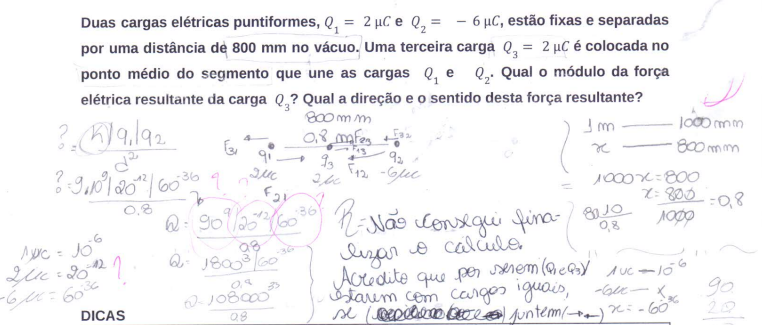
\includegraphics[width=1\textwidth]{fig/mtmasa3.png}
\label{fig:mtmasa3}
\caption*{Fonte: Extraído da produção dos Estudantes.}
\end{center}
\end{figure}

Com base na análise da ASA3, podemos concluir que a etapa que demandou mais auxílio (objetivo \ref{item:b}) foi a de Conteúdo, relacionada ao conhecimento específico da disciplina de Física. No entanto, ao longo do relato, tornou-se evidente que também foi necessário auxílio nas etapas de aplicação matemática. Apesar disso, os alunos não solicitaram esse auxílio por diversos motivos. Portanto, é importante considerar ambas as etapas como pontos de atenção para o desenvolvimento das habilidades dos alunos e garantir que eles se sintam encorajados a buscar ajuda quando necessário.

Com base nas informações do Professor e nos resultados dos alunos, constatamos que somente na última aplicação foi possível verificar uma evolução no processo de RP dos estudantes. No entanto, devido à dificuldade da turma em entender a proposta da ASA desde o início, não temos informações suficientes para responder ao objetivo \ref{item:c} sobre a evolução ao longo do tempo. Essa dificuldade pode ter influenciado os resultados e a compreensão do processo de RP, e destaca a importância de uma abordagem mais clara e direcionada em atividades futuras, para melhor acompanhamento do progresso dos alunos.

\begin{figure}[ht]
\begin{center}
\caption{Exemplo de dicas preferidas ao longo da ASA3.}
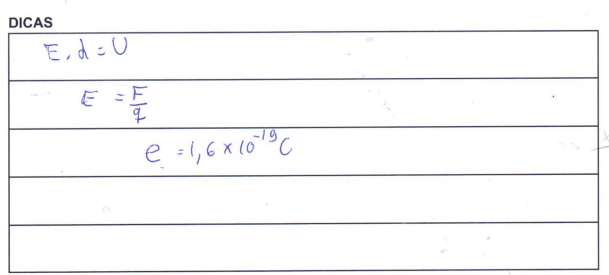
\includegraphics[width=1\textwidth]{fig/didasa3.png}
\label{fig:didiasa3}
\caption*{Fonte: Extraído da produção dos Estudantes.}
\end{center}
\end{figure}

É interessante notar que, de acordo com o relato do Professor, os alunos tinham uma preferência (objetivo \ref{item:d}) por dicas diretas, independentemente do tipo de dica oferecida - como mostrado na Figura \ref{fig:didiasa3}. Essa preferência pode estar relacionada à tentativa dos alunos de resolverem as questões com o mínimo de interferência externa possível. Além disso, eles pareciam estar buscando resolver as questões rapidamente, como se estivessem em uma situação de prova de vestibular, buscando otimizar o tempo disponível. Essa abordagem pode refletir a ansiedade e a pressão que os alunos podem sentir durante as avaliações importantes, como o vestibular, e evidencia a necessidade de equilibrar o uso das dicas com o desenvolvimento da autonomia e confiança dos estudantes em suas habilidades de RP.

\begin{table}[ht]
    \centering
    \caption{Respostas da ASA3 ao questionário final.}\label{tab:questASA3}
    \begin{tabular}{ccccc}
    \hline
       \textbf{Pergunta 1} & \textbf{Pergunta 2} & \textbf{Pergunta 3} & \textbf{Pergunta 4} & \textbf{Pergunta 5} \\ \hline
        1 & 1 & 1 & 4 & 5 \\ 
        3 & 1 & 4 & 1 & 1 \\ 
        4 & 3 & 5 & 2 & 2 \\ 
        5 & 1 & 3 & 3 & 5 \\ 
        3 & 3 & 4 & 2 & 3 \\ 
        5 & 5 & 5 & 3 & 5 \\ 
        3 & 3 & 4 & 4 & 4 \\ 
        5 & 5 & 5 & 4 & 2 \\ 
        3 & 3 & 5 & 1 & 5 \\ 
        5 & 4 & 5 & 3 & 4 \\ 
        5 & 4 & 5 & 4 & 3 \\ 
        5 & 4 & 4 & 3 & 4 \\ \hline
    \end{tabular}
    \caption*{Fonte: Construção do Autor.}
\end{table}

A Tabela \ref{tab:questASA3} apresenta as respostas dadas pelos alunos às perguntas do questionário, utilizando a escala Likert, ao término da aplicação da ASA3. O questionário completo está disponível no Apêndice \ref{ch:questASA}. Essas respostas fornecem informações importantes sobre a percepção dos alunos em relação ao processo de aplicações e suas experiências com a abordagem da ASA3.

Um primeiro fator relevante a ser observado é que 12 dos 14 alunos pesquisados responderam ao questionário, apesar de não ser obrigatório. Essa taxa de resposta corresponde a aproximadamente 86\% dos alunos pesquisados. Esse alto nível de participação indica que os alunos estavam interessados em compartilhar suas percepções e experiências sobre a ASA3, o que fortalece a validade das informações coletadas por meio do questionário.

Sobre o grau de dificuldade das questões (pergunta 1), em geral, a turma da ASA3 concordou que as questões apresentavam semelhança com as propostas em sala de aula. No entanto, os relatos deixados pelos alunos indicam que durante as aplicações eles enfrentavam maiores dificuldades do que costumavam ter ao resolver questões em sala de aula. Essa percepção pode ter contribuído para a redução no número de solicitações de dicas, já que alguns alunos sentiram-se mais desafiados e preferiram testar suas habilidades sem buscar auxílio imediato.

Os alunos se dividiram ao tentar avaliar se a ASA seria uma boa maneira de avaliá-los (pergunta 2). Pelos relatos obtidos, também no questionário (questão dissertativa), muitos alunos não gostam de resolver problemas e prefeririam ter seus conhecimentos avaliados de outras formas.

No entanto, é importante destacar que a RP é uma etapa importante e fundamental para o aprendizado da disciplina de Física, como já foi descrito nesta dissertação. Embora existam outros meios de avaliação, eles são complementares à RP e não podem ser substitutos completos dessa abordagem. Através da RP, os alunos desenvolvem habilidades de raciocínio, pensamento crítico e aplicação prática do conhecimento adquirido em diferentes situações.

Portanto, a ASA se apresenta como uma ferramenta valiosa para auxiliar os estudantes na melhoria de suas competências em RP, e, ao longo do processo, pode contribuir para que eles se sintam mais confiantes e preparados para enfrentar os desafios acadêmicos, incluindo as avaliações de vestibulares e ENEM, que também valorizam a habilidade de resolver problemas de forma eficaz.

Quando perguntados sobre a eficácia das dicas fornecidas durante a RP (pergunta 3), a maioria dos alunos concordou que elas foram úteis. Isso indica que os alunos sentiram que houve uma melhora em seus resultados após fazerem uso das dicas durante o processo de resolução das questões. Essa percepção reforça o papel positivo das dicas na compreensão dos conteúdos e na superação das dificuldades encontradas durante as aplicações da ASA3.

Ao serem questionados sobre o autoconhecimento de suas habilidades e desempenho ao longo das aplicações (pergunta 4), a turma apresentou uma divisão de opiniões, mas com uma leve tendência a concordar que entenderam melhor suas competências e dificuldades. Essa percepção é um fator relevante, pois demonstra que os alunos estão, em parte, se tornando mais conscientes de suas habilidades e áreas em que precisam melhorar. Esse autoconhecimento pode ser um ponto positivo para o aprimoramento do aprendizado, uma vez que permite que eles identifiquem suas forças e fraquezas e busquem formas de aperfeiçoar suas habilidades.


De acordo com as respostas dos alunos à pergunta sobre a possibilidade de haver mais aplicações ao longo do trimestre, a turma, em geral, concordou com essa ideia. Isso indica que a maioria dos estudantes gostaria de repetir esse processo mais vezes. 

Essa aceitação pode estar conectada ao fato de que os alunos levaram um tempo para compreender como o processo da ASA pode auxiliá-los em seu aprendizado. Com o passar do tempo e a experiência com as aplicações, eles perceberam os benefícios desse método e, consequentemente, demonstraram interesse em tê-lo mais vezes no decorrer do trimestre para aprimorar suas habilidades e superar dificuldades.

Com base na análise do questionário, é possível afirmar que o interesse na RP não apenas se manteve ao longo do trimestre (objetivo \ref{item:e}), mas também aumentou. Essa constatação pode ser atribuída às boas experiências que os alunos tiveram ao participar das aplicações da ASA e após compreenderem a forma de funcionamento desse método de aprendizagem. A medida em que os alunos se familiarizaram com o processo e perceberam os benefícios das aplicações, o interesse e a motivação para se engajar no processo de RP foram fortalecidos, demonstrando um crescente engajamento com o método ao longo do trimestre.

\chapter{Considerações Finais} \label{ch:conclusao}

Este trabalho foi desenvolvido no âmbito do EDR, uma abordagem de pesquisa que busca encontrar soluções práticas para problemas reais no contexto da educação. Nessa perspectiva, nosso objetivo foi analisar a competência de RP em Física, utilizando a metodologia de \textit{Scaffolding} como uma ferramenta de apoio ao processo de aprendizagem dos alunos. Essa metodologia oferece suporte estruturado e gradual aos estudantes, auxiliando-os no desenvolvimento de habilidades necessárias para resolver problemas de forma autônoma e eficiente.

A ideia inicial do projeto, concebida em meados de 2019, precisou ser adaptada para uma nova realidade trazida pela Pandemia de coronavírus. Esse processo resultou na implementação da ORP1 em uma turma de Engenharia Civil, utilizando o formato de aulas remotas.

Durante todo o processo de coleta de dados, enfrentamos uma série de desafios que merecem destaque. Tanto durante a realização da ORP1 quanto nas aplicações subsequentes, a influência da pandemia foi manifesta em nossas atividades.

Durante a ORP1, vivenciamos o auge da pandemia de forma direta, o que nos obrigou a adotar um ambiente de ensino remoto. Nas ORP2, ORP3 e nas ASA, pudemos observar que os períodos de aulas remotas e isolamento social tiveram um impacto direto no desenvolvimento dos alunos, especialmente aqueles do nível médio, nas ASA.

É fundamental salientar que este estudo foi conduzido em um período de tempo singular, no qual os resultados obtidos possivelmente teriam sido diferentes se não tivéssemos enfrentado uma situação tão complexa de saúde pública em escala global.

Durante a primeira aplicação da metodologia de \textit{Scaffolding}, diversos aspectos prejudicaram uma análise mais completa e precisa. Entre esses aspectos, destacam-se a perda das respostas dos questionários dos alunos, o impacto da Pandemia que afetou tanto o formato de aulas remotas quanto o aspecto psicológico dos estudantes, e a identificação de possíveis casos de plágio nas resoluções dos alunos. Esses fatores dificultaram a obtenção de informações valiosas e confiáveis para uma análise mais aprofundada da eficácia da metodologia em questão.

A perda das respostas dos questionários dos alunos representou uma limitação significativa para a compreensão de suas percepções e opiniões sobre a experiência com a metodologia de \textit{Scaffolding}. Sem esses dados, tornou-se mais desafiador entender como os alunos reagiram ao processo de ensino e aprendizagem, e quais pontos específicos poderiam ser aprimorados ou adaptados para melhor atender suas necessidades.

Além disso, a situação da Pandemia trouxe impactos significativos para o ambiente educacional e para o bem-estar dos estudantes. A transição abrupta para o ensino a distância pode ter gerado desafios adicionais para o envolvimento e a motivação dos alunos, afetando suas experiências de aprendizagem e a interação com a metodologia proposta.

Outro aspecto que exigiu atenção foi a identificação de semelhanças suspeitas nas resoluções dos alunos. Essas similaridades indicavam a possibilidade de plágio, o que trouxe desafios para a análise da autenticidade das respostas e a confiabilidade dos resultados obtidos. Esse foi um fator que precisou ser considerado para garantir a integridade acadêmica do processo de avaliação. 

Diante dos desafios e limitações encontrados na primeira aplicação da metodologia de \textit{Scaffolding}, foi necessário realizar um \textit{redesign} do projeto para continuar a análise de forma mais apropriada. Esse novo \textit{design}, alinhado com os princípios do EDR, resultou em duas novas aplicações: ORP2 e ORP3. 

As novas aplicações, ORP2 e ORP3, foram realizadas simultaneamente em turmas de cursos de Matemática e Física. Além dos objetivos gerais a serem analisados, também surgiu o interesse em investigar as possíveis diferenças entre essas turmas, uma composta por estudantes novatos e outra por especialistas em Física, durante o processo de RP.

Devido ao baixo número de alunos matriculados nas disciplinas da ORP2 e ORP3, a análise comparativa entre as turmas e outros objetivos não puderam ser completamente elucidados. Diante disso, optou-se por um novo \textit{redesign} da metodologia, direcionado para turmas do Ensino Médio. 

A metodologia ASA foi implementada simultaneamente em três turmas distintas do Ensino Médio: uma no 1º ano, outra no 2º ano e uma terceira no 3º ano de uma Escola Particular e Confessional localizada no interior do Estado do Rio Grande do Sul. Apesar das turmas possuírem conhecimentos semelhantes em relação à Física, as particularidades e características individuais de cada grupo de alunos mostraram-se bastante distintas. Essas diferenças podem influenciar na forma como os alunos abordam e enfrentam os desafios das aplicações da ASA.

A turma do 1º ano demonstrou interesse em participar da metodologia da ASA. No entanto, seus resultados e relatos do Professor indicam que a dedicação aos estudos foi insuficiente. Muitos alunos pareciam depender demasiadamente das dicas fornecidas ao longo das aplicações, na esperança de obterem uma boa nota sem um esforço mais aprofundado de estudo. Essa atitude pode ter afetado o desempenho geral da turma na ASA.

A turma do 2º ano apresentou uma divisão significativa em relação à participação nas aplicações da ASA. Muitos alunos enfrentavam dificuldades, mas não solicitavam ajuda, o que pode indicar uma falta de engajamento nos estudos fora de sala de aula. Como resultado, os desempenhos individuais não foram considerados satisfatórios pela escola. Essa falta de engajamento pode ter influenciado diretamente nos resultados alcançados .

A turma do 3º ano apresentou uma peculiaridade em relação à sua percepção sobre a ASA ao longo do processo. Inicialmente, eles não entenderam a função dessas atividades no seu processo de aprendizagem, o que levou a uma visão equivocada sobre a finalidade da ASA. Como estavam preocupados com as provas de vestibular e ENEM que enfrentariam no final do ano, essa percepção distorcida pode ter influenciado na forma como abordaram e interagiram com as aplicações. À medida que a compreensão sobre a importância da ASA se desenvolveu, suas atitudes podem ter se alterado, refletindo-se nos resultados obtidos ao final do processo.

Apesar de termos realizado uma análise detalhada dos objetivos em cada aplicação das ORP e das ASA no Capítulo \ref{ch:resanddisc}, torna-se necessário uma síntese geral desses objetivos. Com esse propósito, apresentamos na Tabela \ref{tab:objetivosResp} nossa análise das respostas dos objetivos específicos deste trabalho, abrangendo todas as aplicações realizadas nos diferentes \textit{designs}.

\begin{table}[ht]
\centering
\caption{Análise dos Objetivos Específicos}
\label{tab:objetivosResp}
\begin{tabular}{l p{10cm}}
\hline
\textbf{Objetivo \ref{item:a}} & Os alunos que obtiveram sucesso na resolução dos problemas propostos seguiram passos similares aos de \citeonline{Pozo2009}. \\
\hline
\textbf{Objetivo \ref{item:b}} & As etapas em que as dicas são fornecidas variam consideravelmente, mas são frequentes nas dúvidas relacionadas a Conteúdo e Matemática. \\
\hline
\textbf{Objetivo \ref{item:c}} & A evolução temporal é um processo individual de cada estudante, sendo necessário analisá-la dentro de um estudo de caso para obter uma compreensão mais detalhada e específica. Dessa forma, este objetivo não foi alcançado. \\
\hline
\textbf{Objetivo \ref{item:d}} & As formas mais eficientes de dicas para a compreensão dos alunos podem variar de acordo com o tipo de dica fornecida. No entanto, dicas transmitidas de forma mais objetiva parecem agradar mais aos estudantes. \\
\hline
\textbf{Objetivo \ref{item:e}} & O interesse dos alunos na RP depende da compreensão da metodologia. Quando entendem a proposta, se engajam; caso contrário, a veem como "perda de tempo". \\
\hline
\end{tabular}
\caption*{Fonte: Criação do Autor.}
\end{table}

É relevante salientar que a abordagem de RP proposta por \citeonline{Pozo2009}, conforme abordado no objetivo \ref{item:a}, nunca foi instruída diretamente aos alunos. Eles a empregam de forma natural, possivelmente influenciados pela forma como outras pessoas, como pais ou professores, resolvem problemas. Essa influência pode levá-los a adaptar seu processo de resolução, aproximando-o do que é considerado mais adequado.

Adicionalmente, constatou-se que vários dos objetivos traçados inicialmente exibiram variações conforme as circunstâncias e particularidades de cada aluno e turma. Nesse sentido, sugere-se que estudos de caso mais abrangentes e prolongados sejam conduzidos no futuro, permitindo uma investigação mais aprofundada das questões relacionadas ao processo de RP em diferentes contextos educacionais.

Com base nas informações e experiências vivenciadas ao longo de todo o processo, desde a ORP1 até a ASA3, evidencia-se que a metodologia de \textit{Scaffolding} demonstra contribuições significativas para o desenvolvimento da competência de RP em Física. Contudo, existe espaço para aprimorar as estratégias de aplicação, a fim de obter resultados mais abrangentes e abordar uma maior variedade de grupos estudados. 

Recomendamos que o próximo \textit{redesign} seja planejado com um acompanhamento mais prolongado de um indivíduo ou grupo. No contexto de uma turma do Ensino Médio, seria vantajoso acompanhar o progresso da mesma ao longo de um ano letivo, pois um período de tempo mais extenso provavelmente revelaria uma evolução mais significativa no desempenho dos alunos ao final do processo. Isso possibilitaria uma análise mais aprofundada das mudanças ao longo do tempo, identificando padrões de desenvolvimento e áreas de melhoria na competência de RP em Física.

No contexto do Ensino Superior, o acompanhamento individual de um aluno se torna mais viável, devido à natureza das disciplinas, que geralmente são oferecidas de forma individualizada, e à variação das turmas entre diferentes disciplinas. Dessa maneira, torna-se possível acompanhar o estudante por mais de um semestre, permitindo uma análise mais aprofundada e prolongada de seu processo de evolução.

Acredita-se que, no Ensino Superior, o diploma de graduação possa servir como um fator motivacional relevante para os estudantes, uma vez que a conclusão do curso é um objetivo claro e almejado para a maioria deles. No entanto, no Ensino Médio, a motivação dos alunos muitas vezes está mais voltada para a obtenção de boas notas do que para o próprio aprendizado em si. 

Nesse contexto, para promover uma melhor interação dos alunos do Ensino Médio com o processo de aplicação da metodologia \textit{Scaffolding}, sugere-se desvincular a aplicação da metodologia de uma avaliação puramente baseada em notas. Em vez disso, é importante explorar outras abordagens para atrair os estudantes para o processo de RP e, consequentemente, para a utilização da metodologia.
%
%% REFERENCIAS
%
\postextual
\bibliography{postextual/ref.bib}
%
%% APENDICES 
%
\begin{apendicesenv}
\chapter{Aplicações da ORP 1}\label{ch:orp1}
\section{Atividade Síncrona 1}\label{ch:orp1e1}
\vspace*{\fill}
\begin{figure}[H]\centering
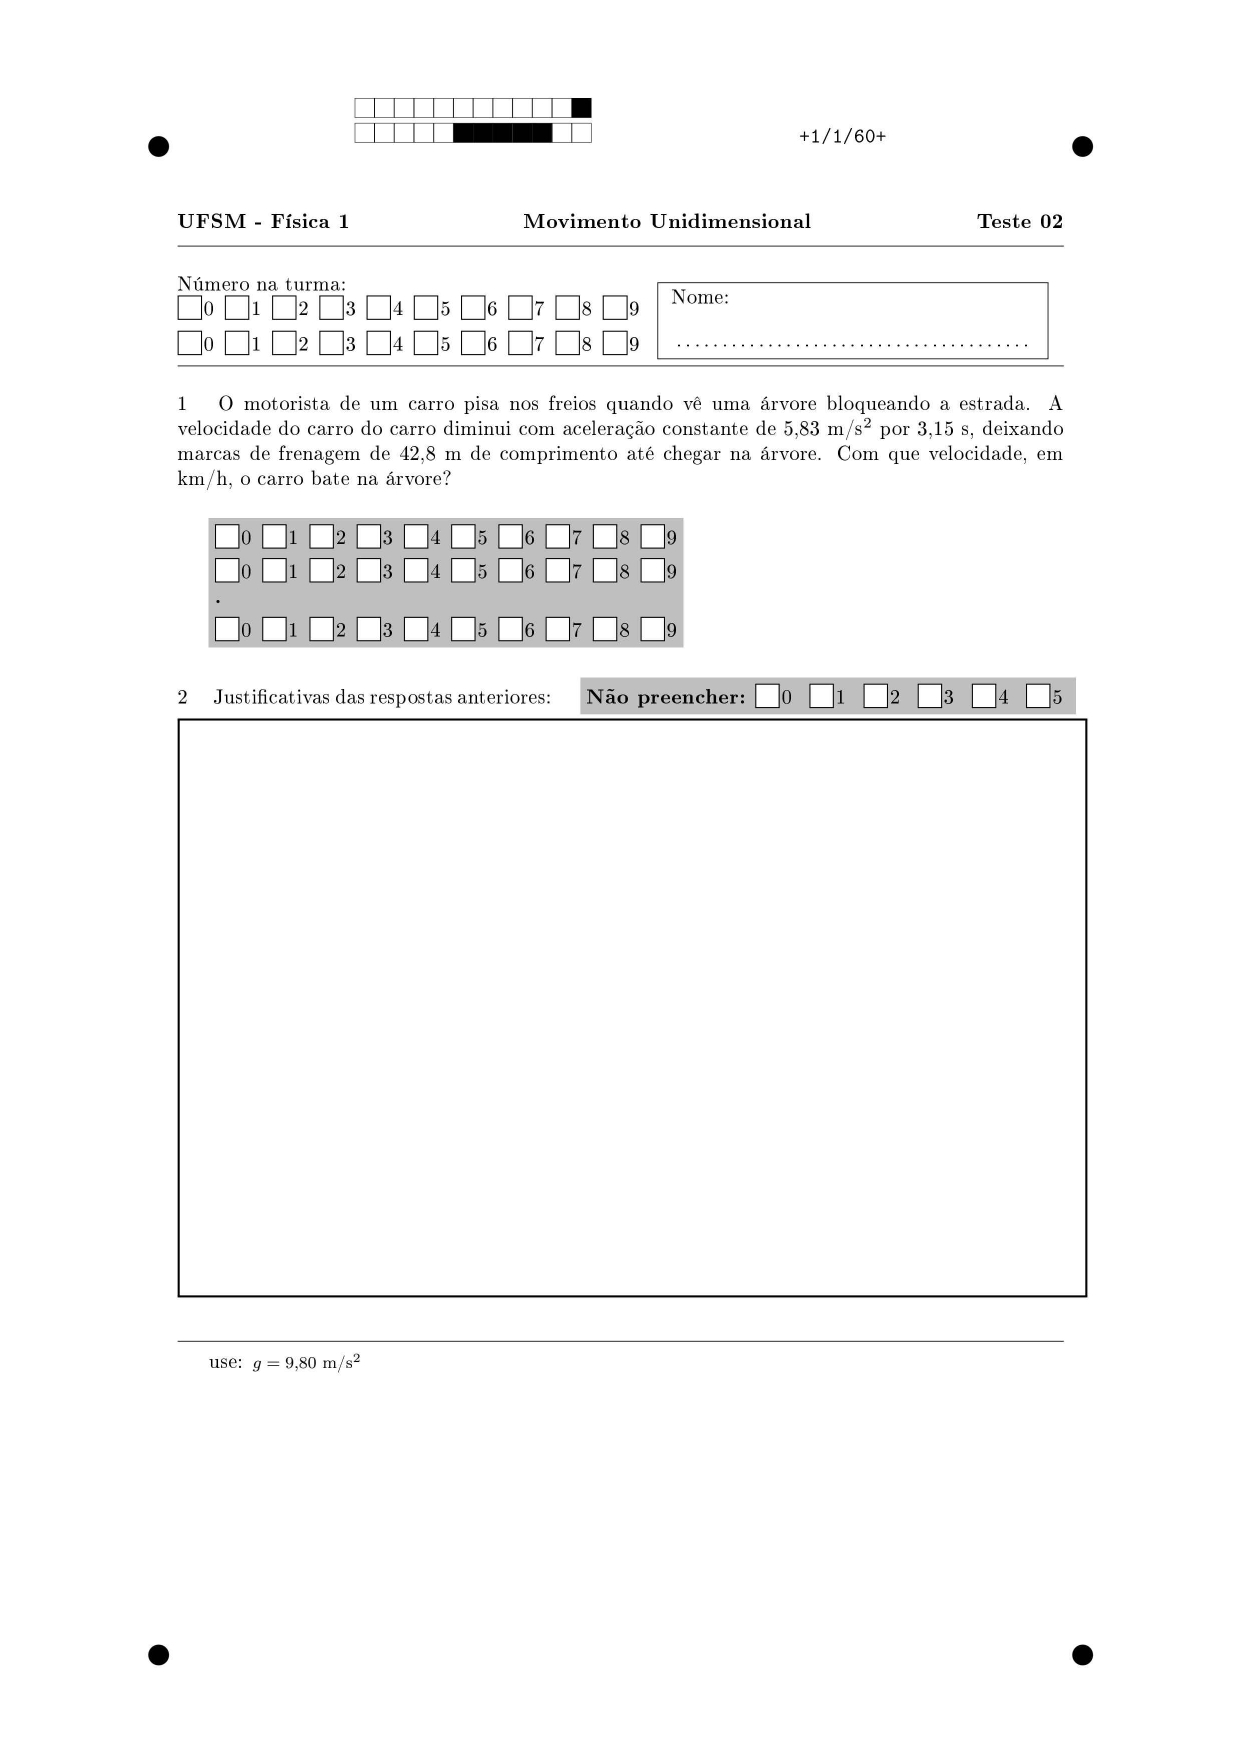
\includegraphics[scale=0.7]{fig/orp1q1_page-0001.jpg}
\end{figure}
\vspace*{\fill}
\begin{figure}[H]\centering
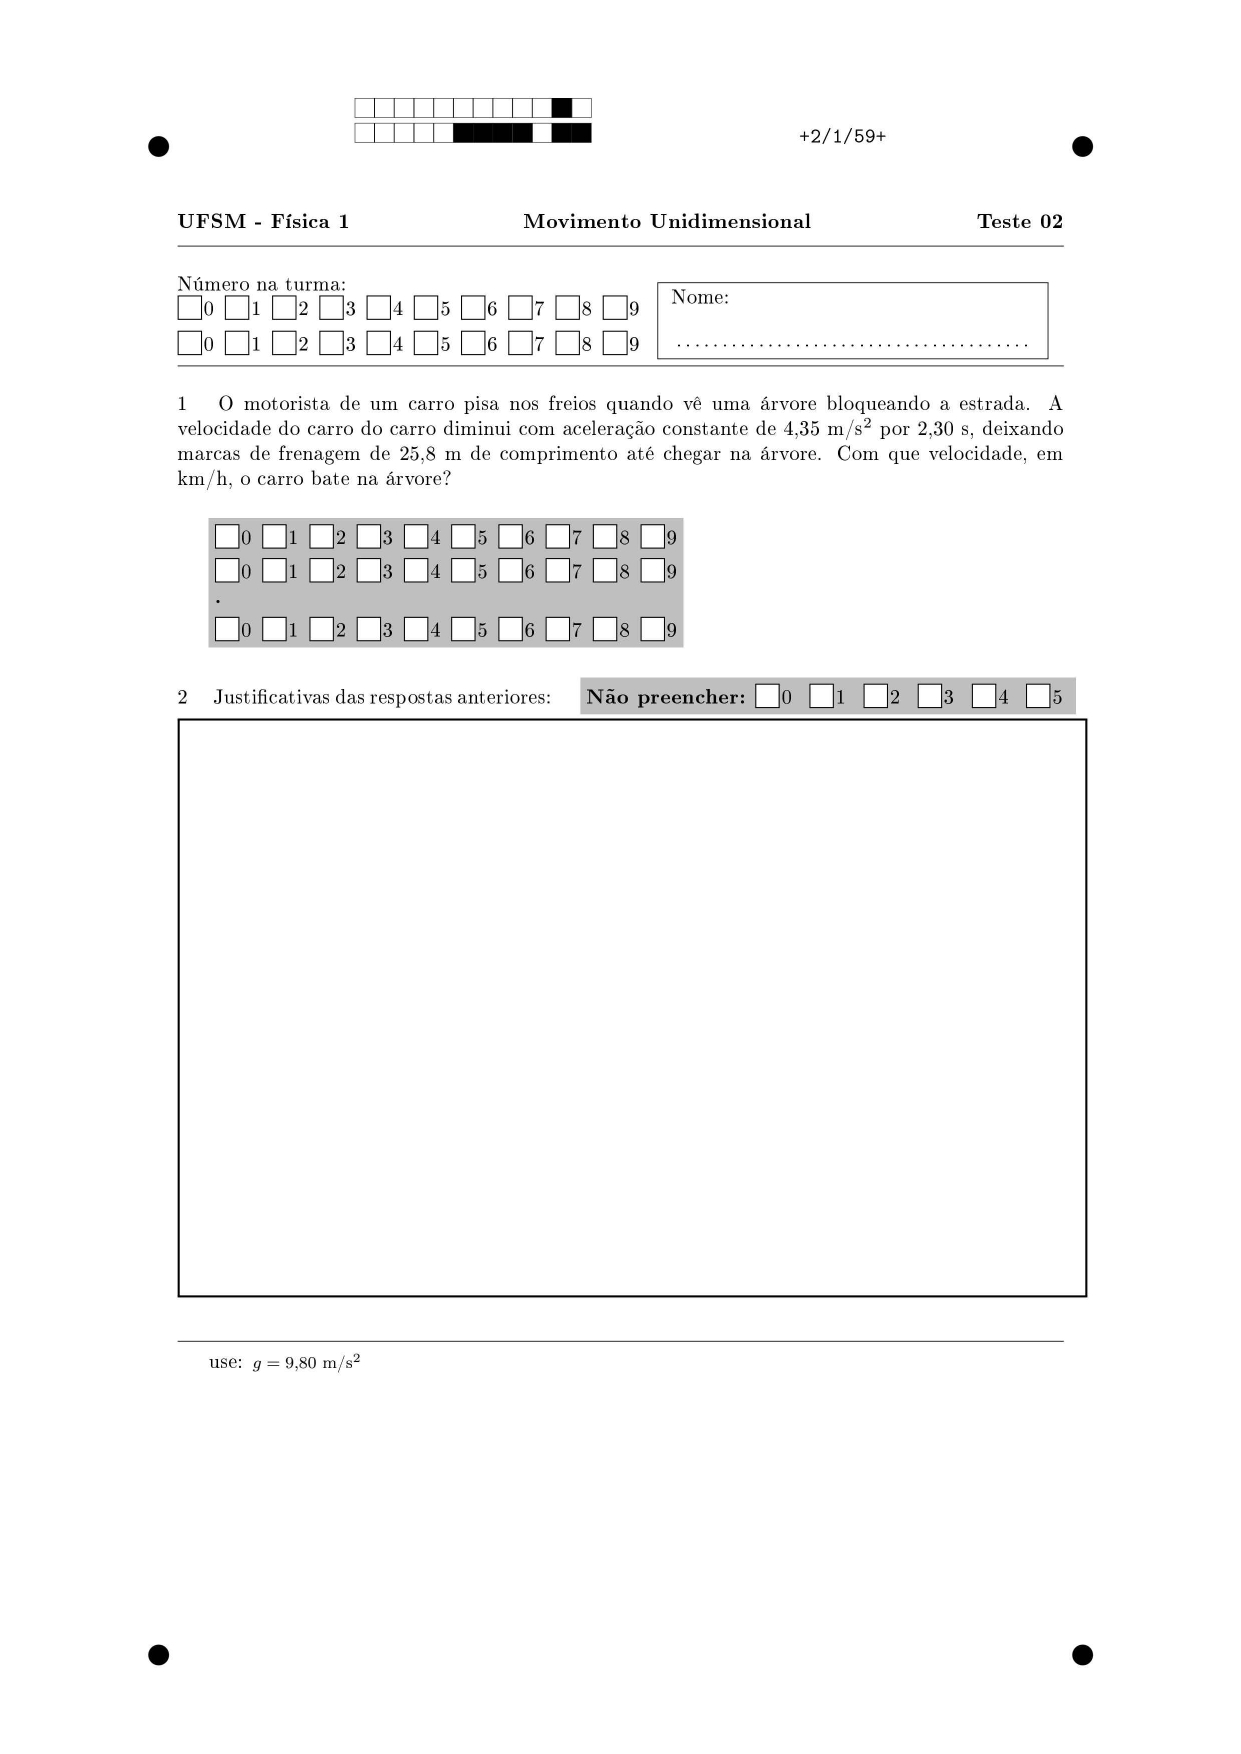
\includegraphics[scale=0.7]{fig/orp1q1_page-0002.jpg}
\end{figure}
\vspace*{\fill}
\begin{figure}[H]\centering
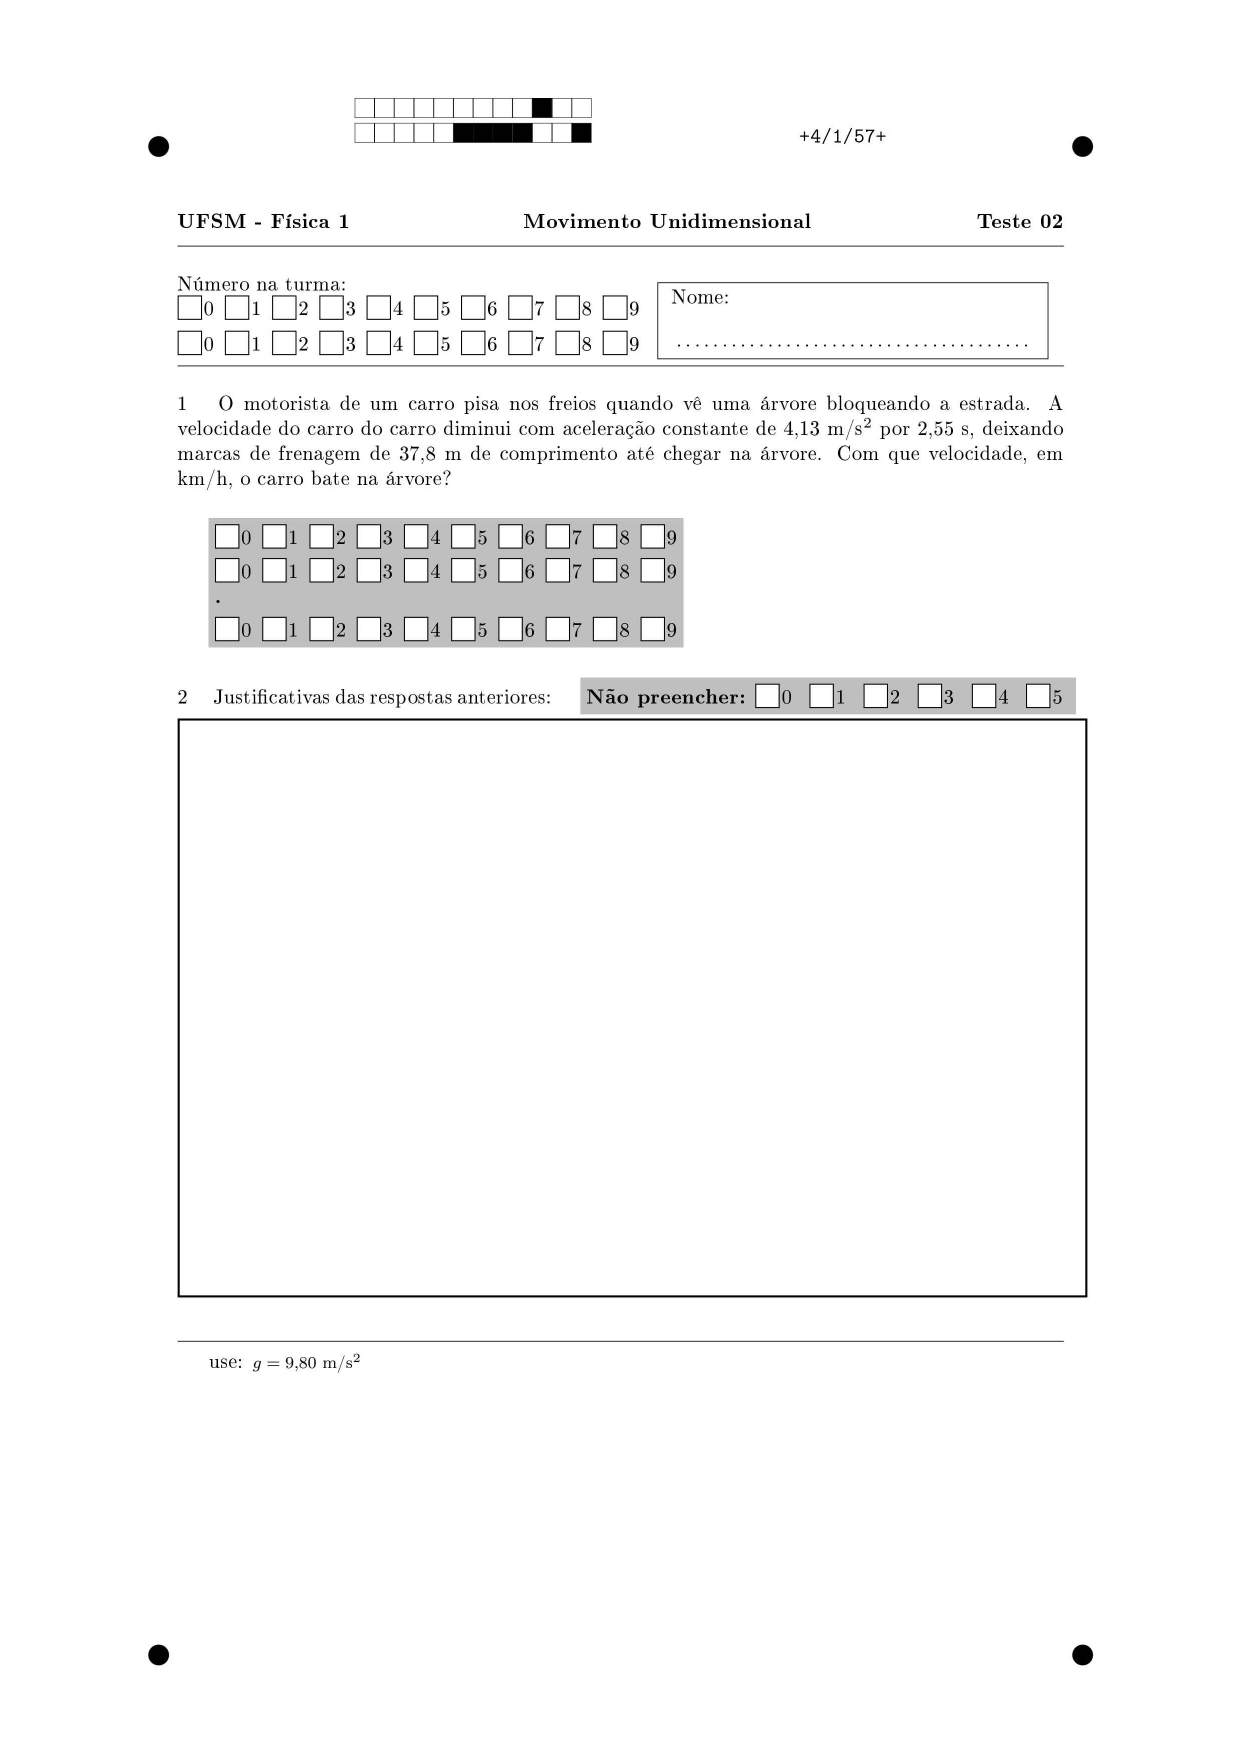
\includegraphics[scale=0.7]{fig/orp1q1_page-0004.jpg}
\end{figure}

\section{Atividade Síncrona 2} \label{ch:orp1e2}
\vspace*{\fill}
\begin{figure}[H]\centering
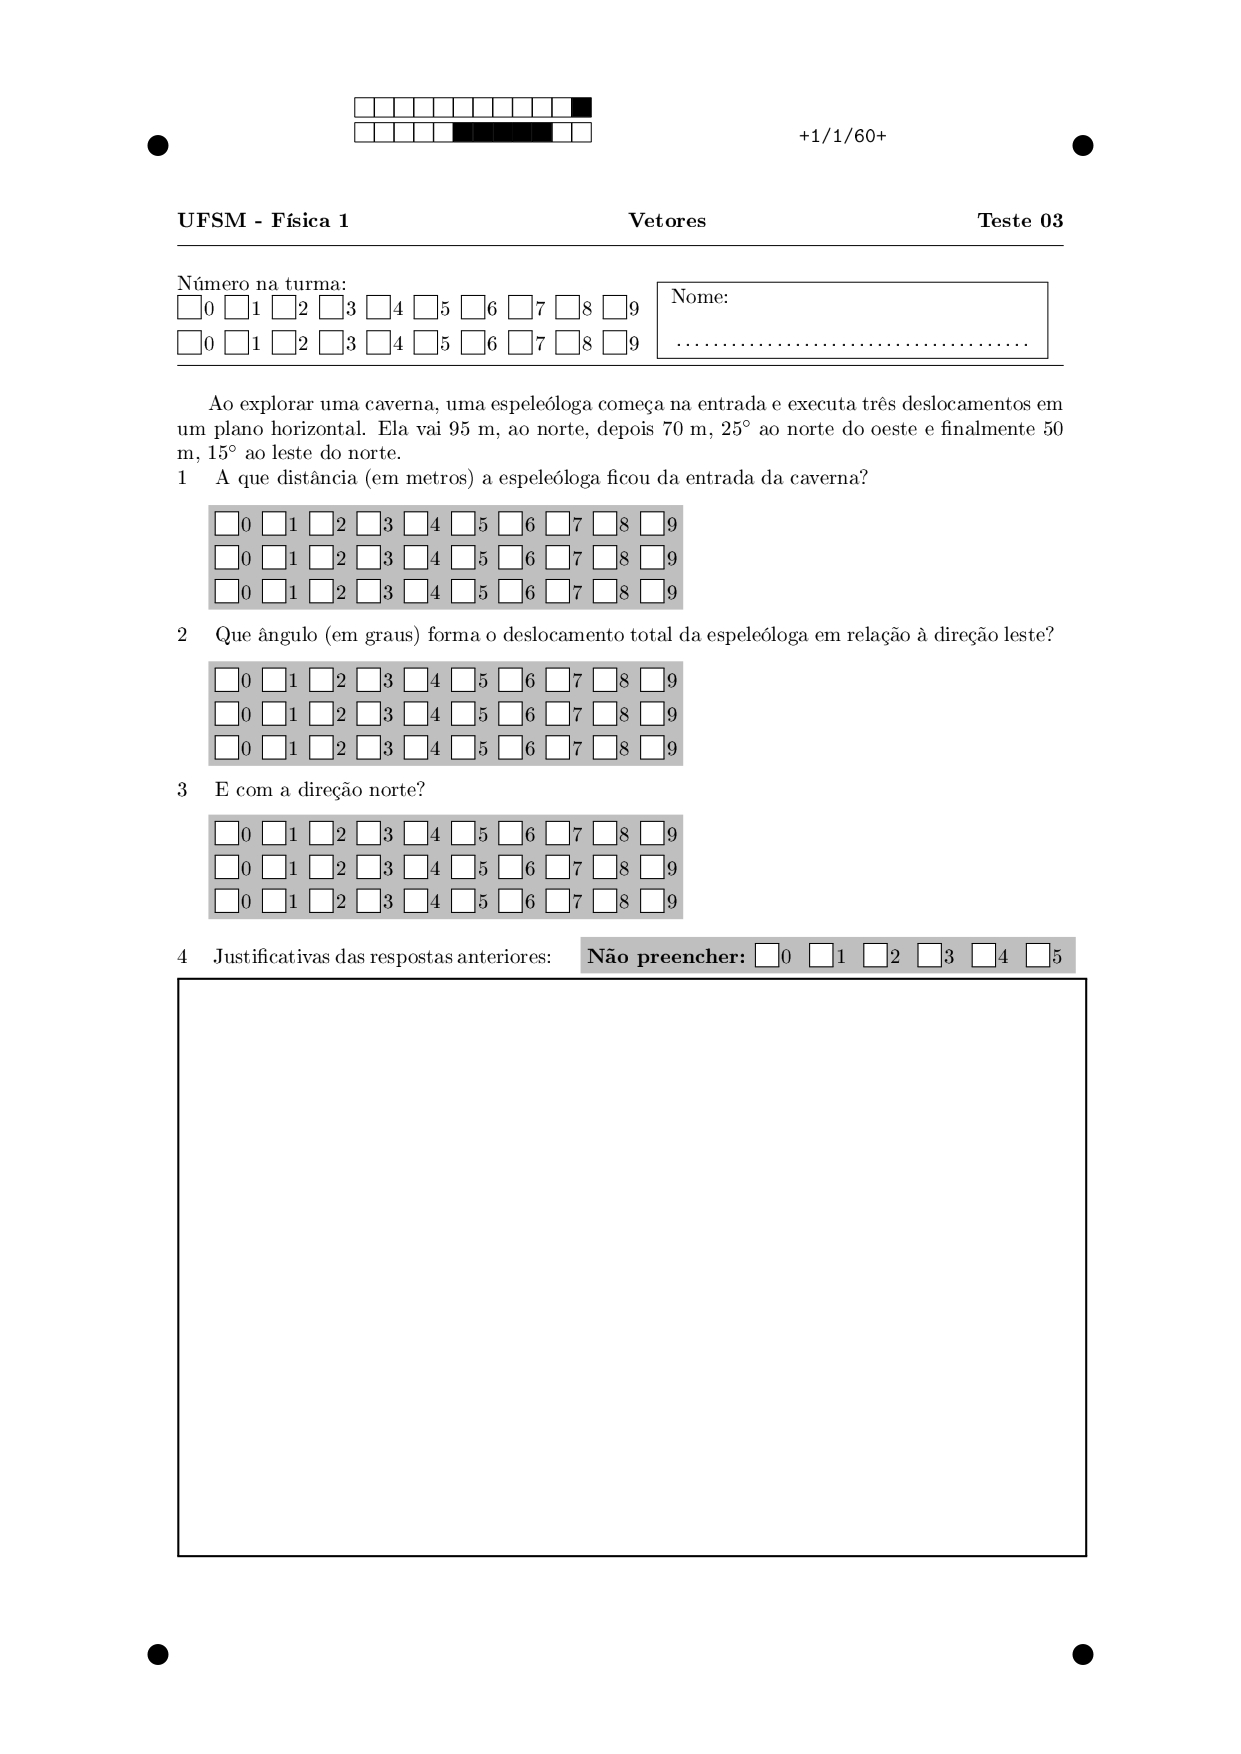
\includegraphics[scale=0.7]{fig/orp1q2_page-0001.jpg}
\end{figure}
\vspace*{\fill}
\begin{figure}[H]\centering
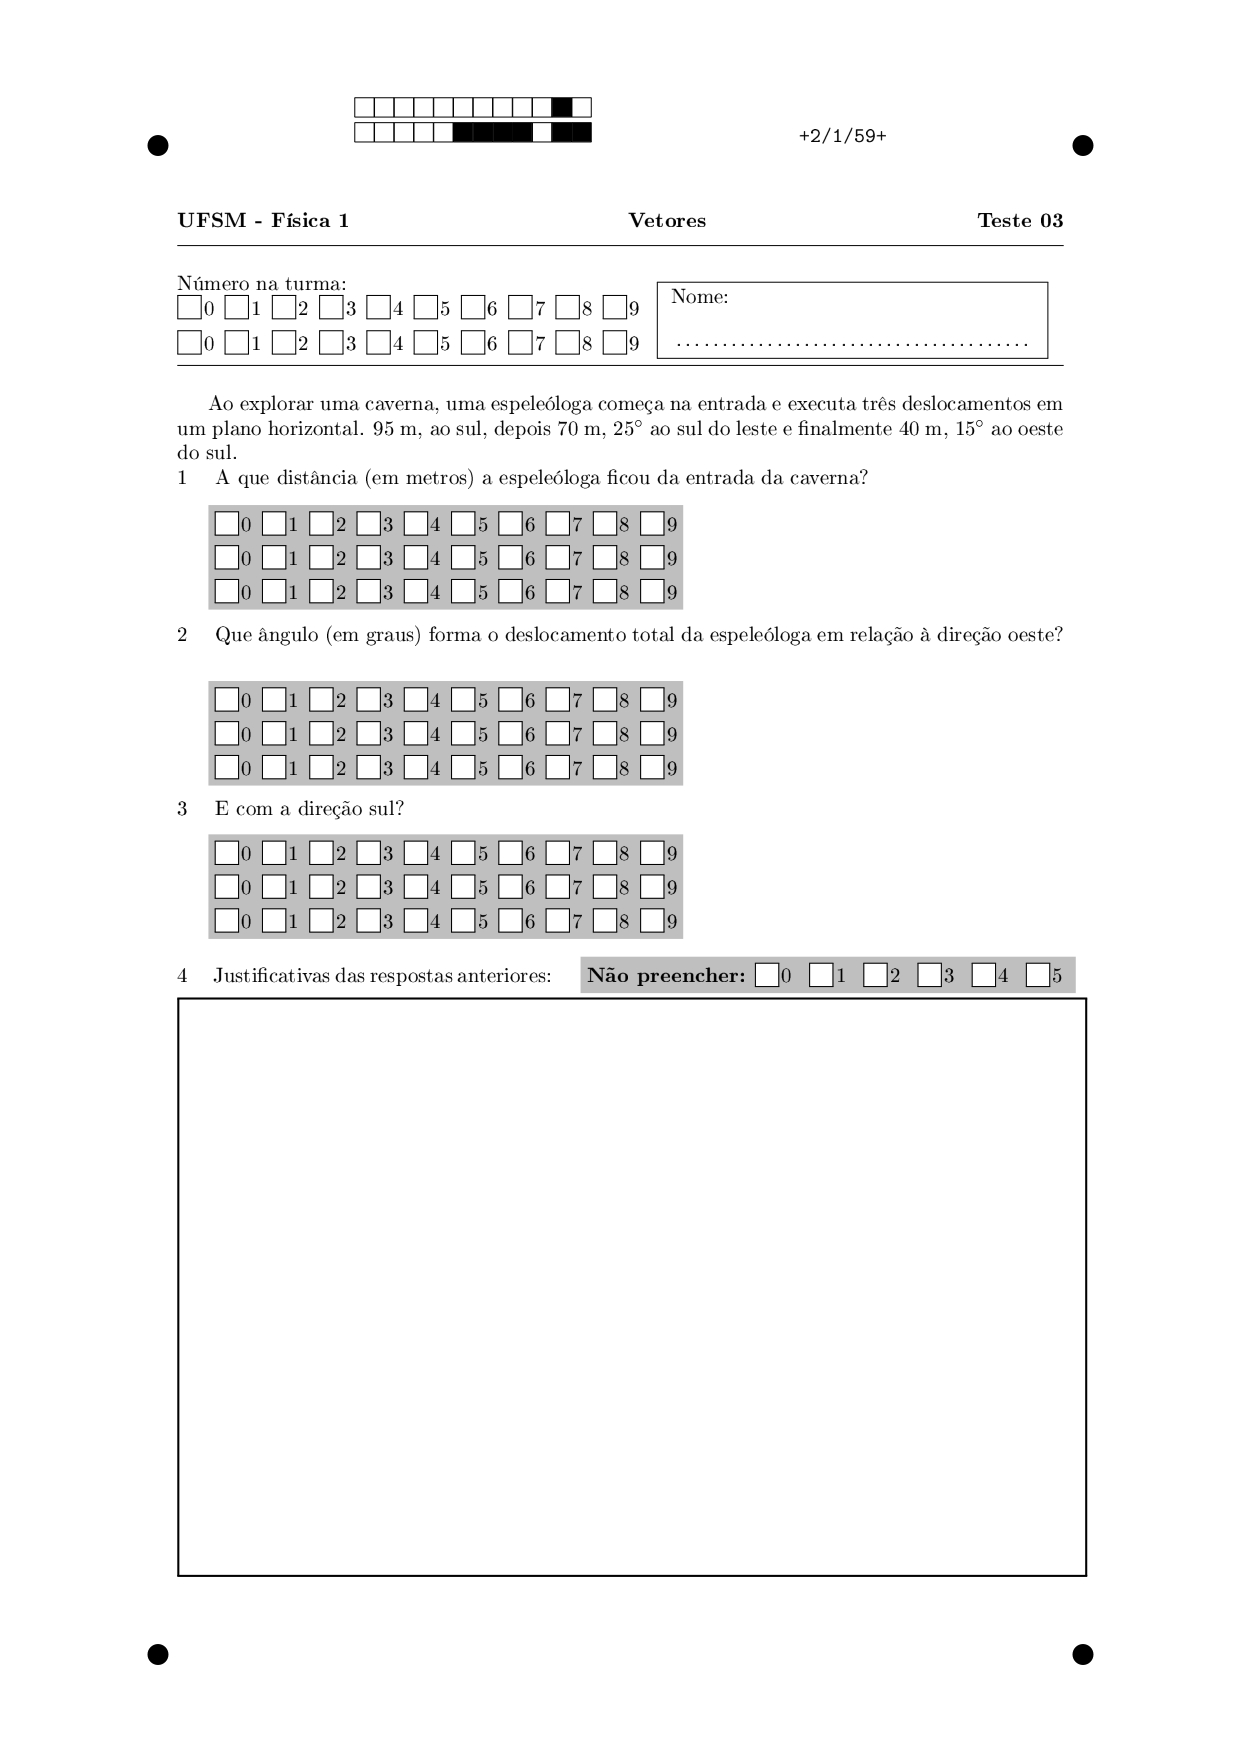
\includegraphics[scale=0.7]{fig/orp1q2_page-0002.jpg}
\end{figure}
\vspace*{\fill}
\begin{figure}[H]\centering
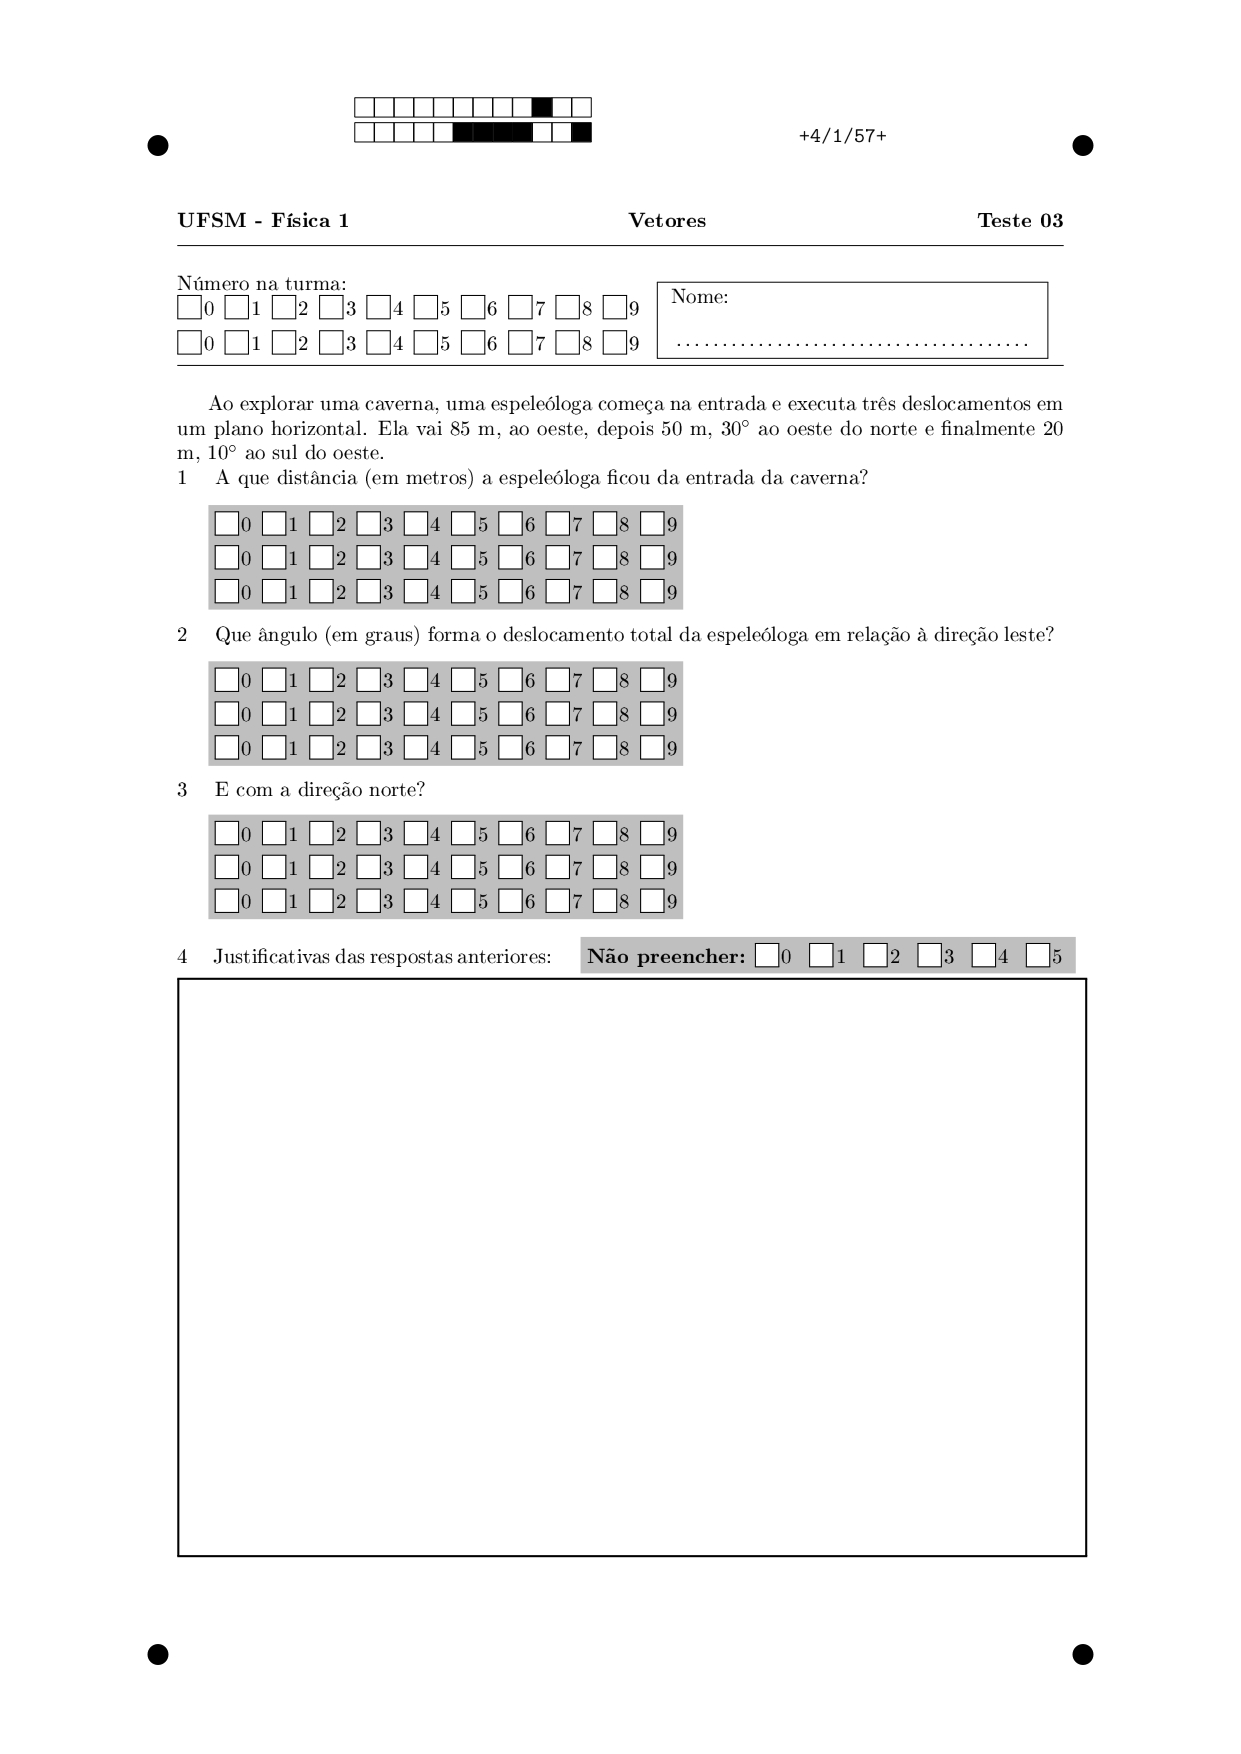
\includegraphics[scale=0.7]{fig/orp1q2_page-0004.jpg}
\end{figure}

\section{Atividade Síncrona 3} \label{ch:orp1e3}
\vspace*{\fill}
\begin{figure}[H]\centering
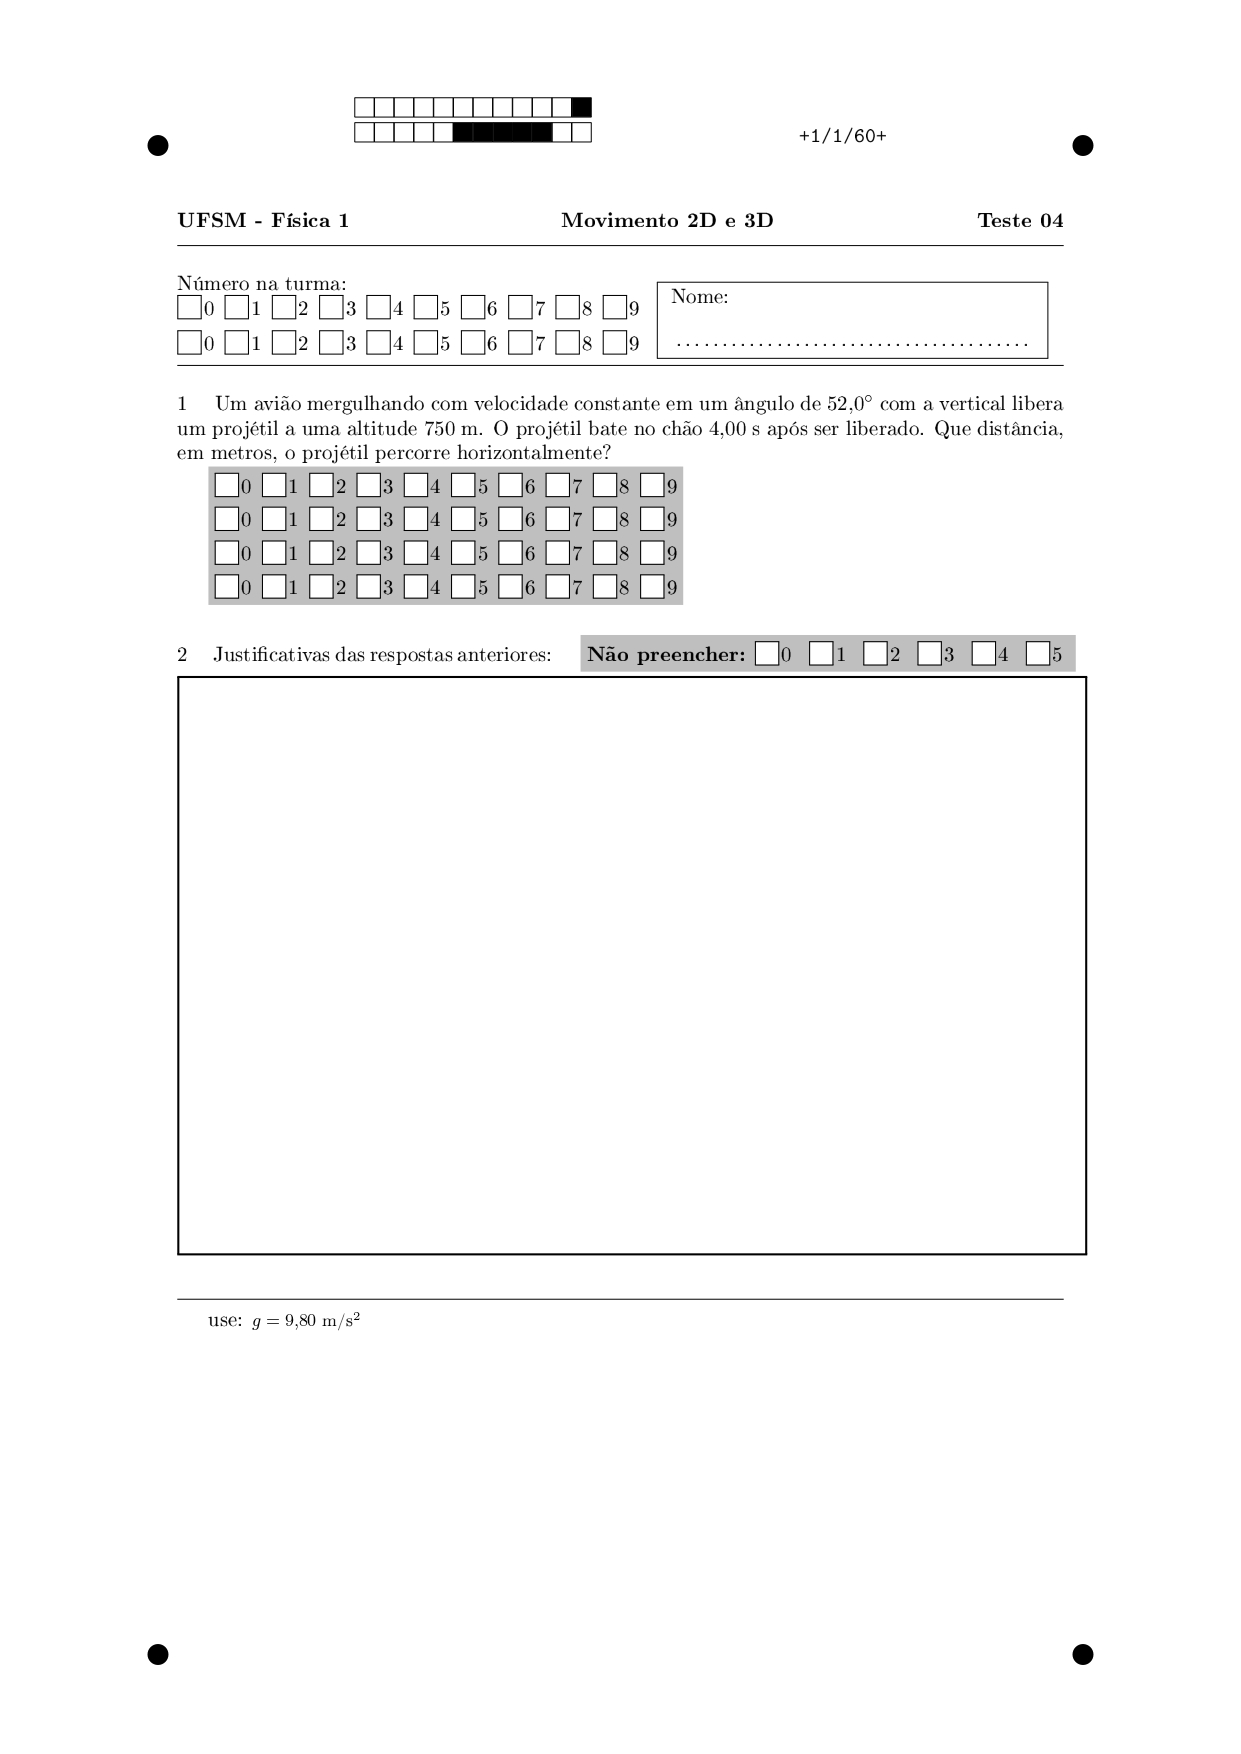
\includegraphics[scale=0.7]{fig/orp1q3r_page-0001.jpg}
\end{figure}
\vspace*{\fill}
\begin{figure}[H]\centering
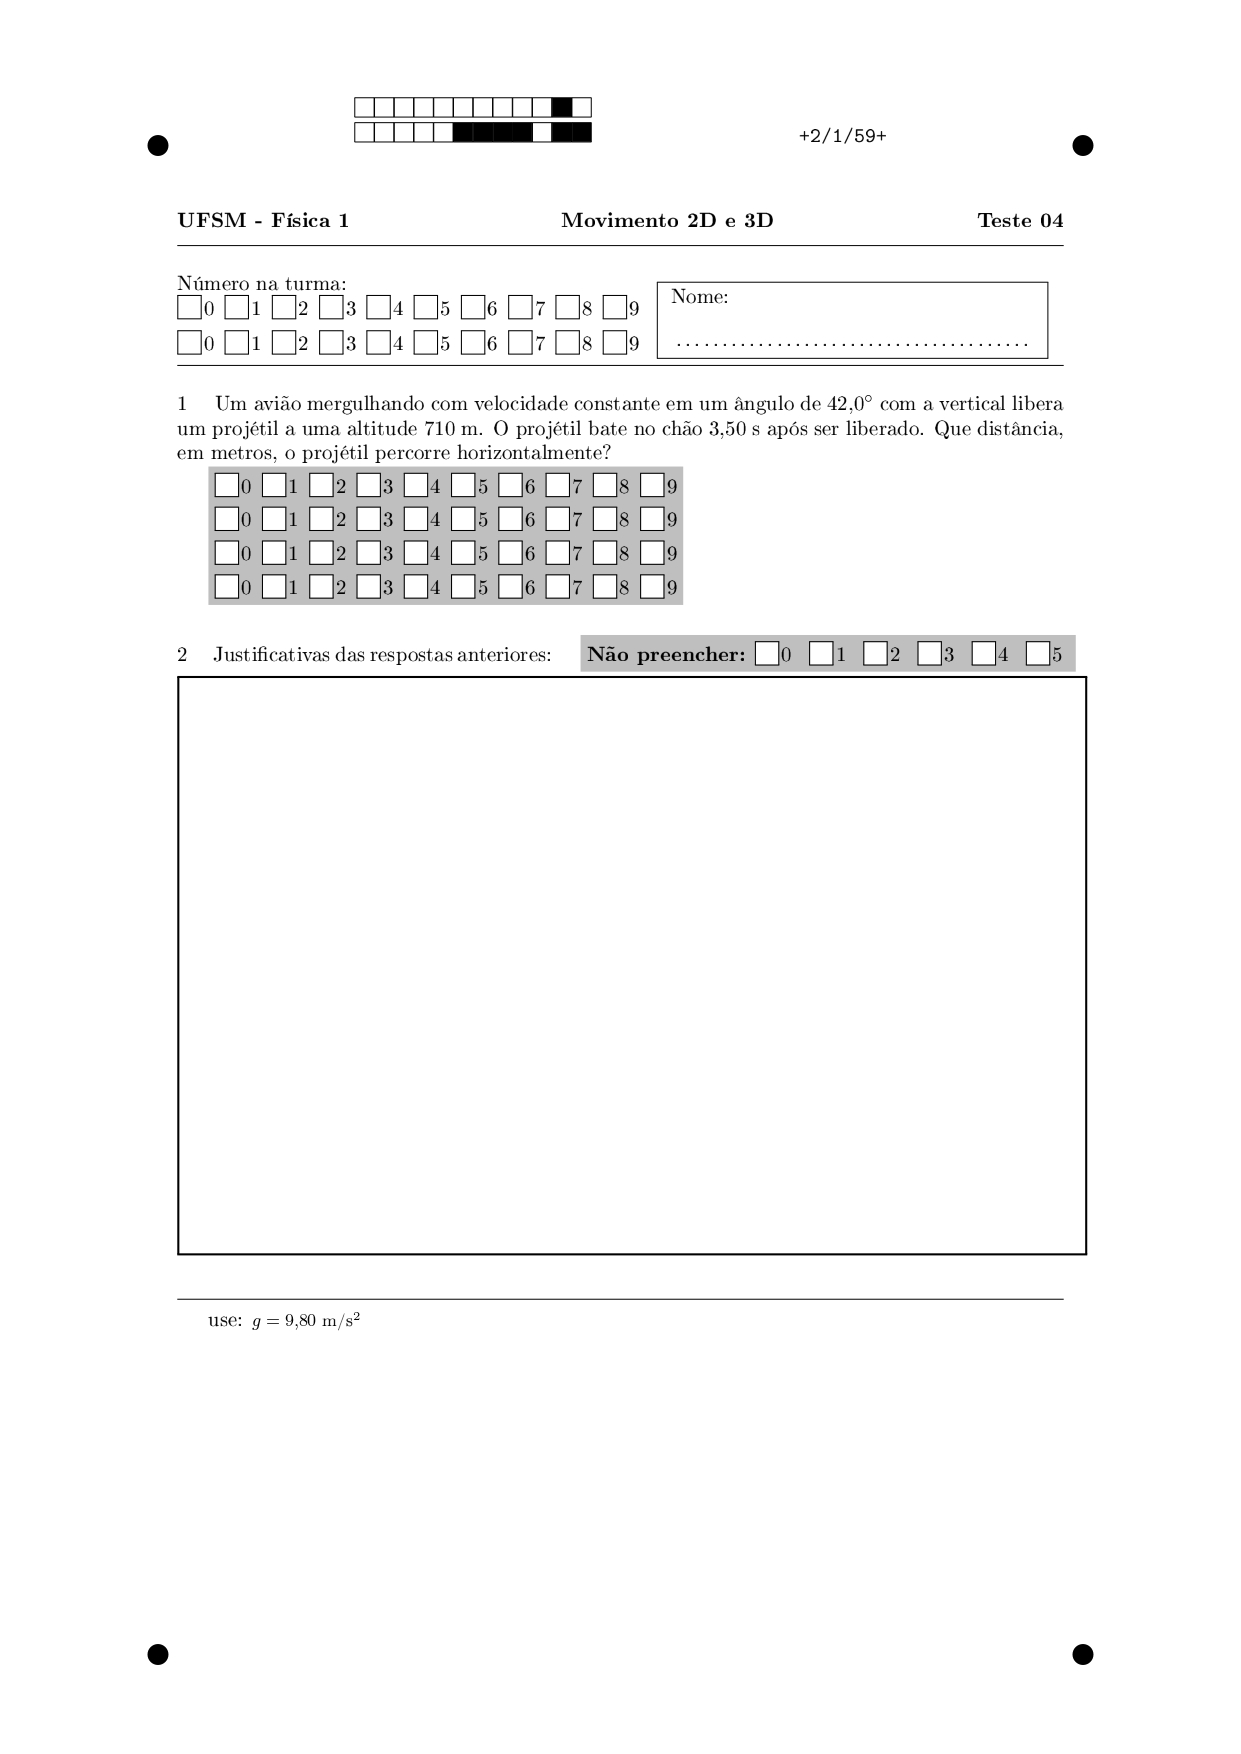
\includegraphics[scale=0.7]{fig/orp1q3r_page-0002.jpg}
\end{figure}
\vspace*{\fill}
\begin{figure}[H]\centering
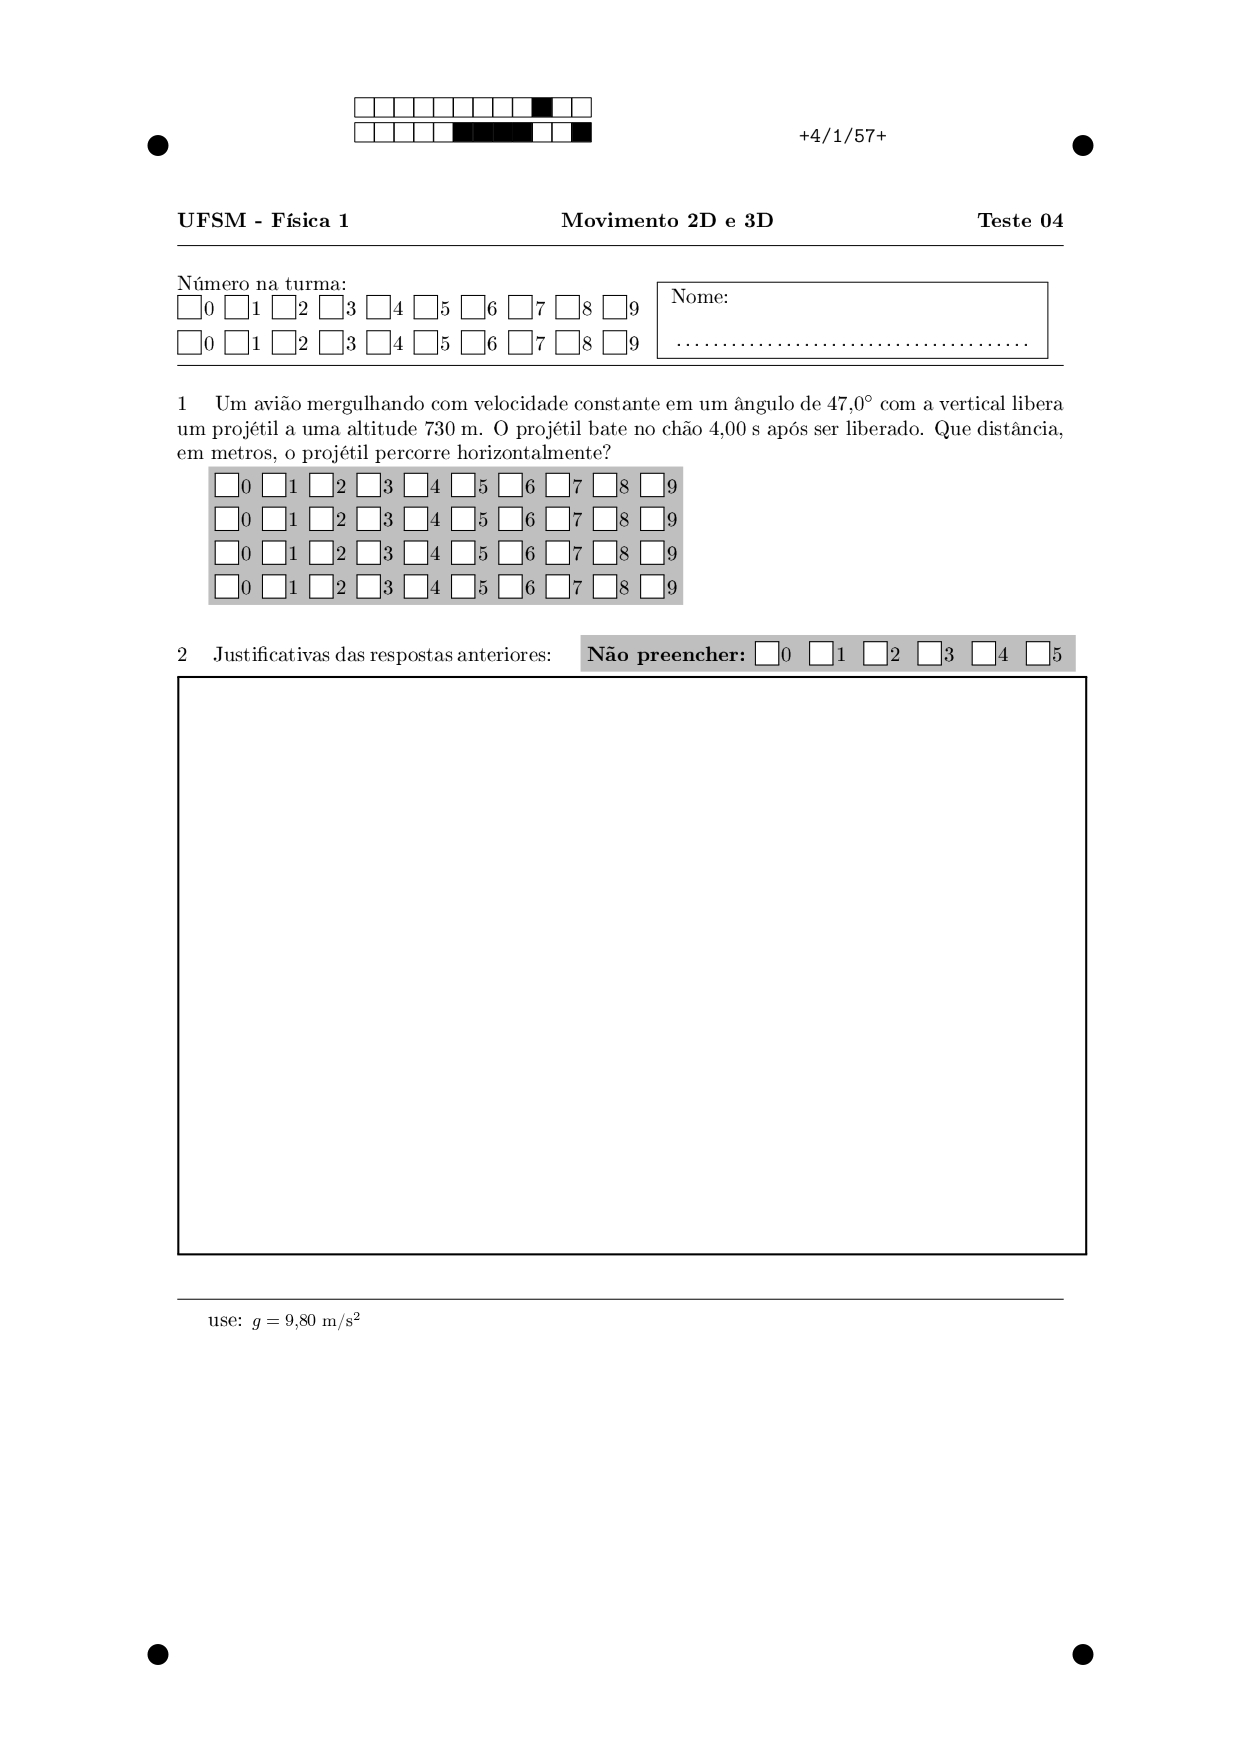
\includegraphics[scale=0.7]{fig/orp1q3r_page-0004.jpg}
\end{figure}

\section{Atividade Síncrona 4} \label{ch:orp1e4}
\vspace*{\fill}
\begin{figure}[H]\centering
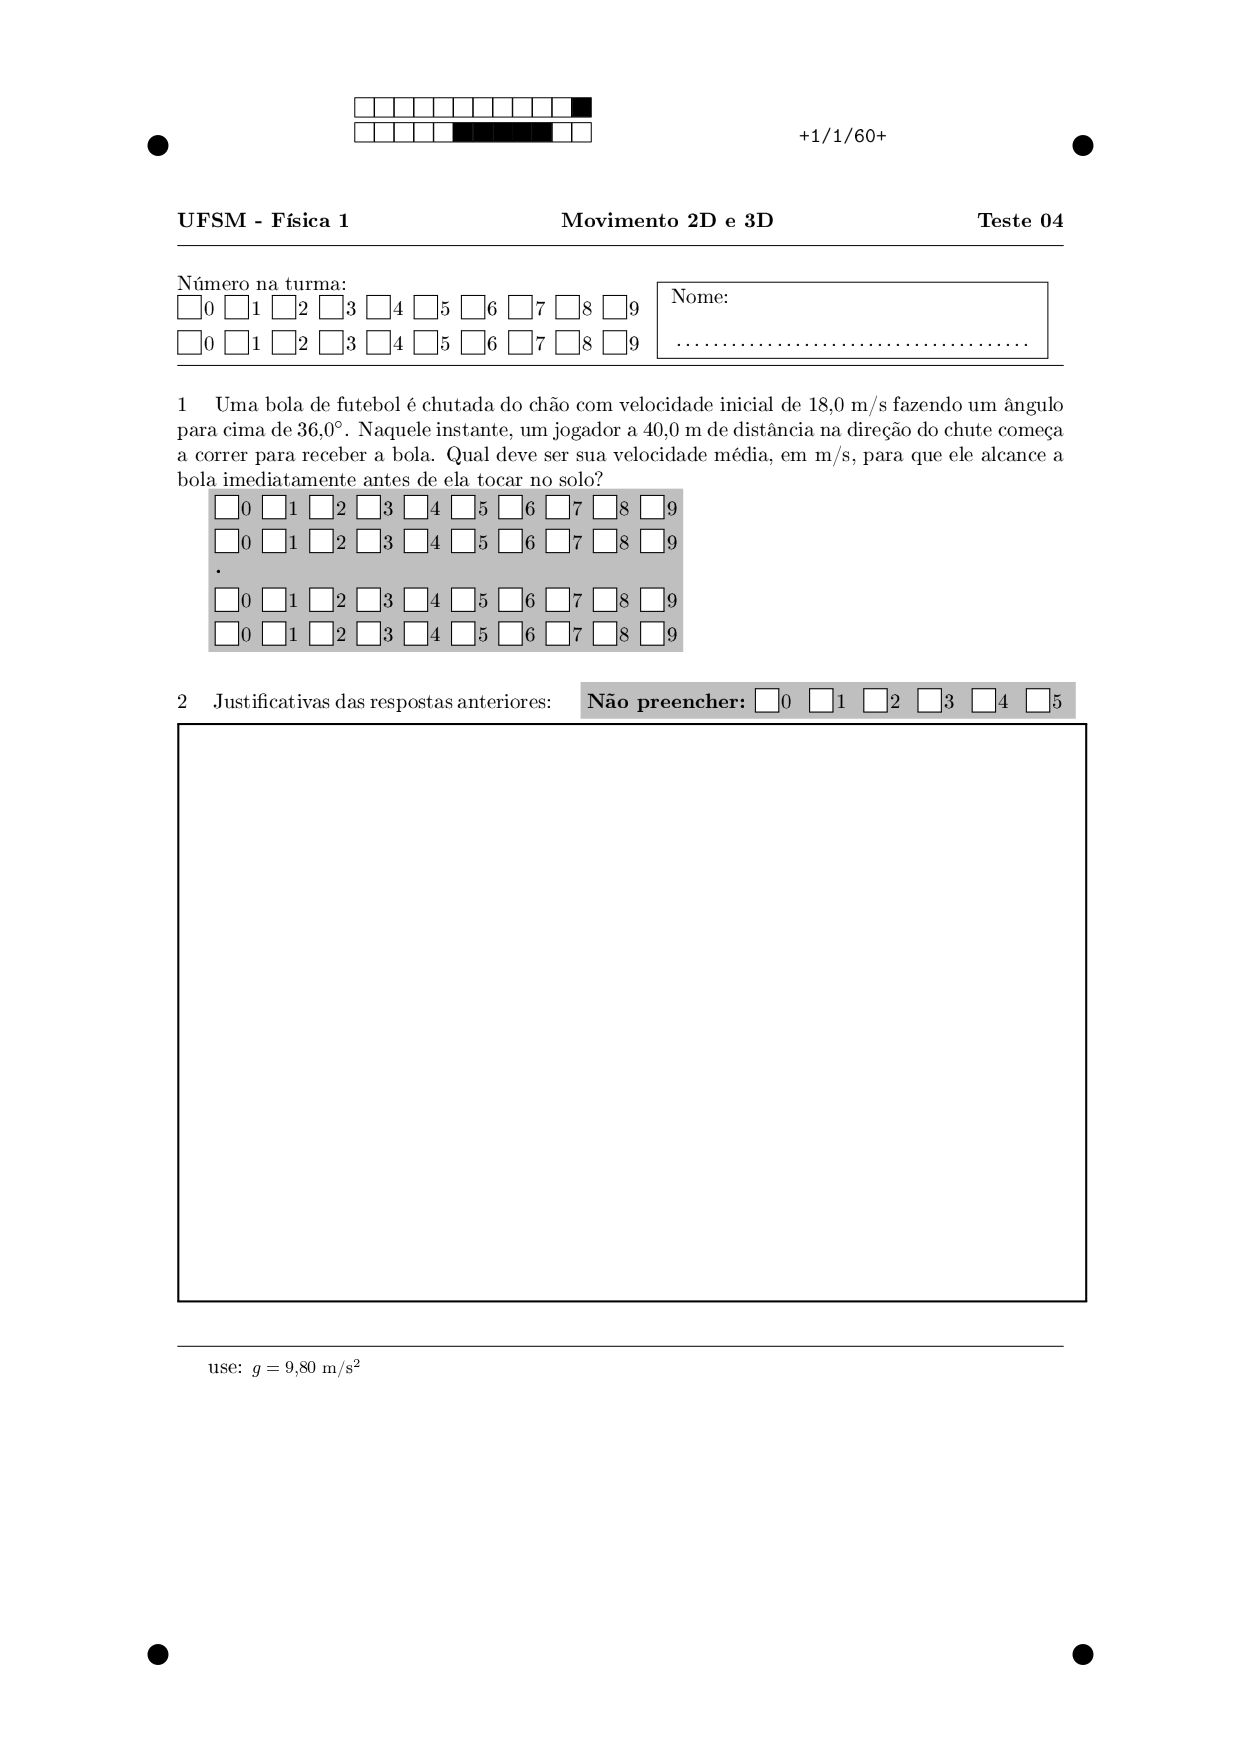
\includegraphics[scale=0.7]{fig/orp1q3_page-0001.jpg}
\end{figure}
\vspace*{\fill}
\begin{figure}[H]\centering
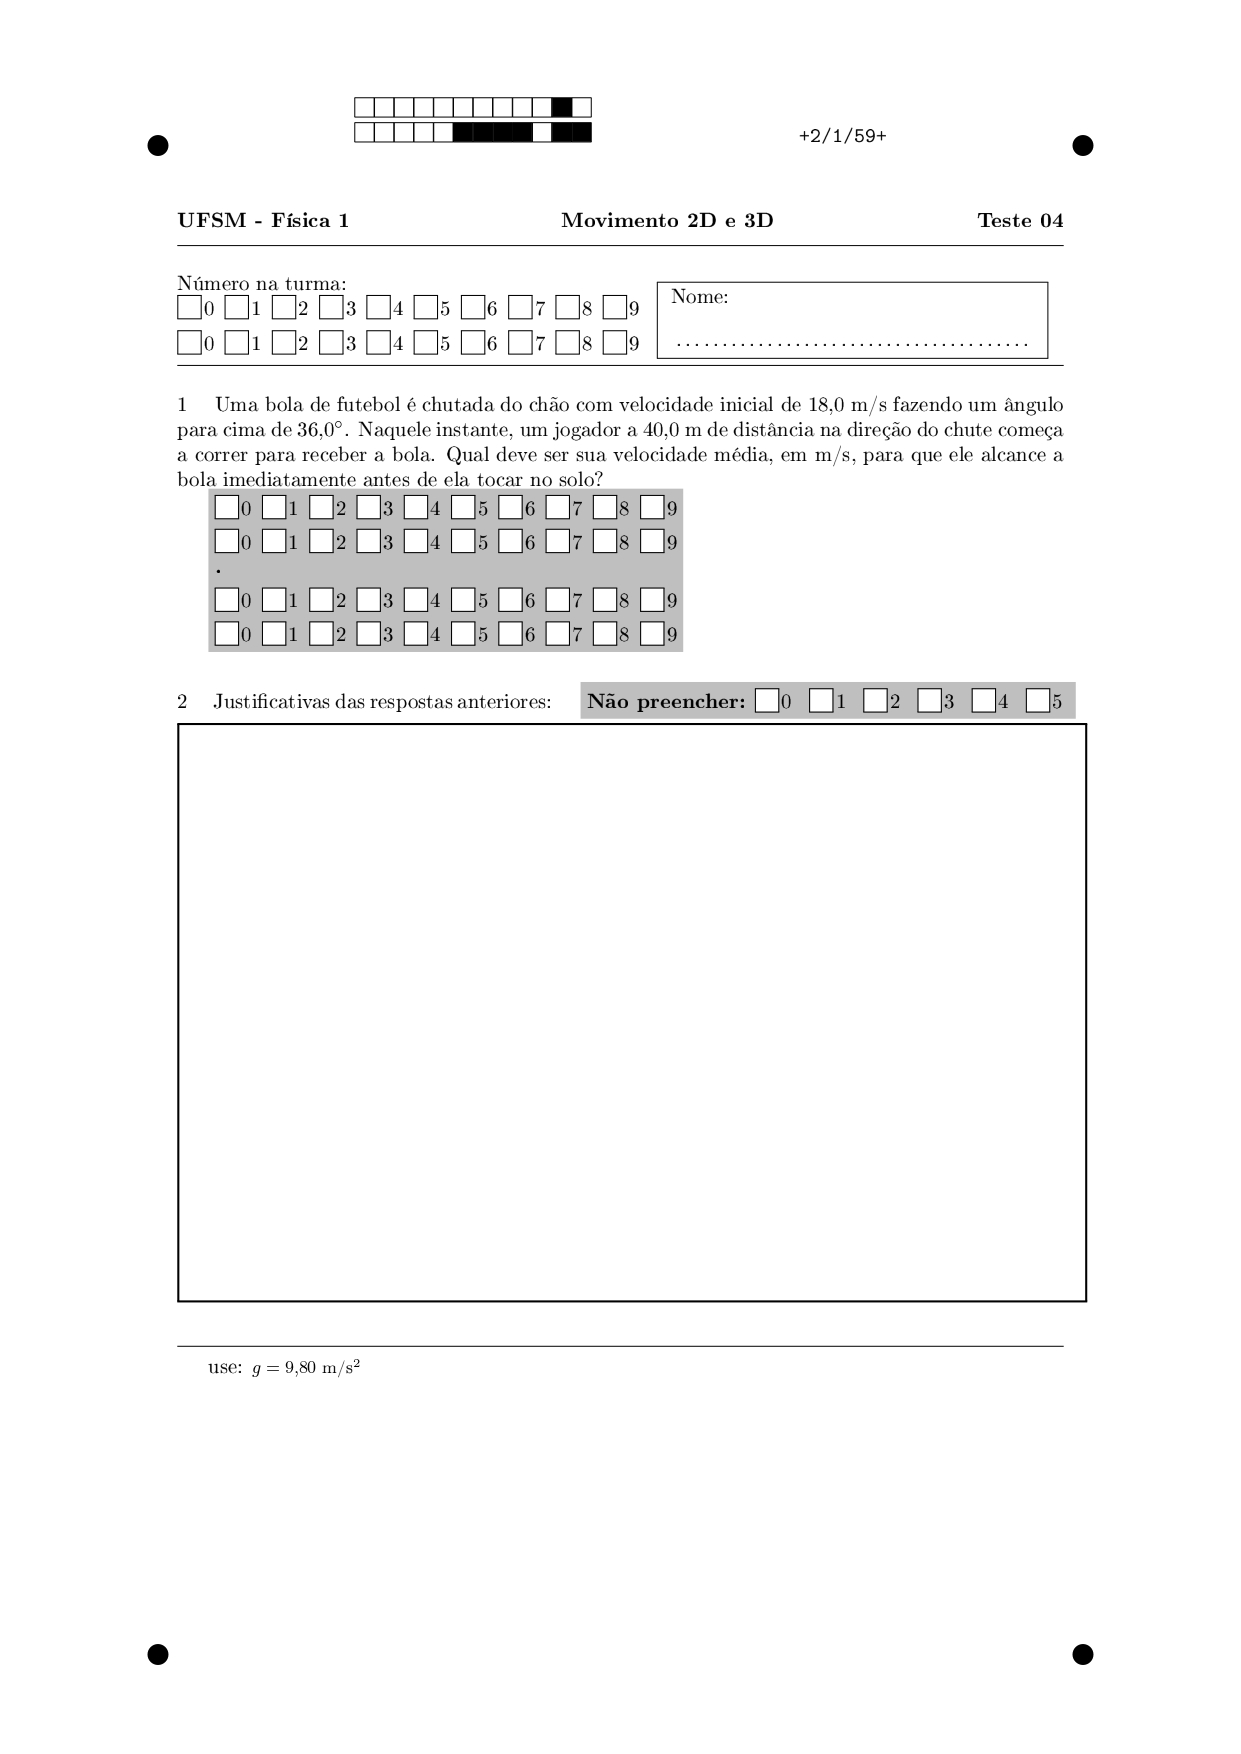
\includegraphics[scale=0.7]{fig/orp1q3_page-0002.jpg}
\end{figure}
\vspace*{\fill}
\begin{figure}[H]\centering
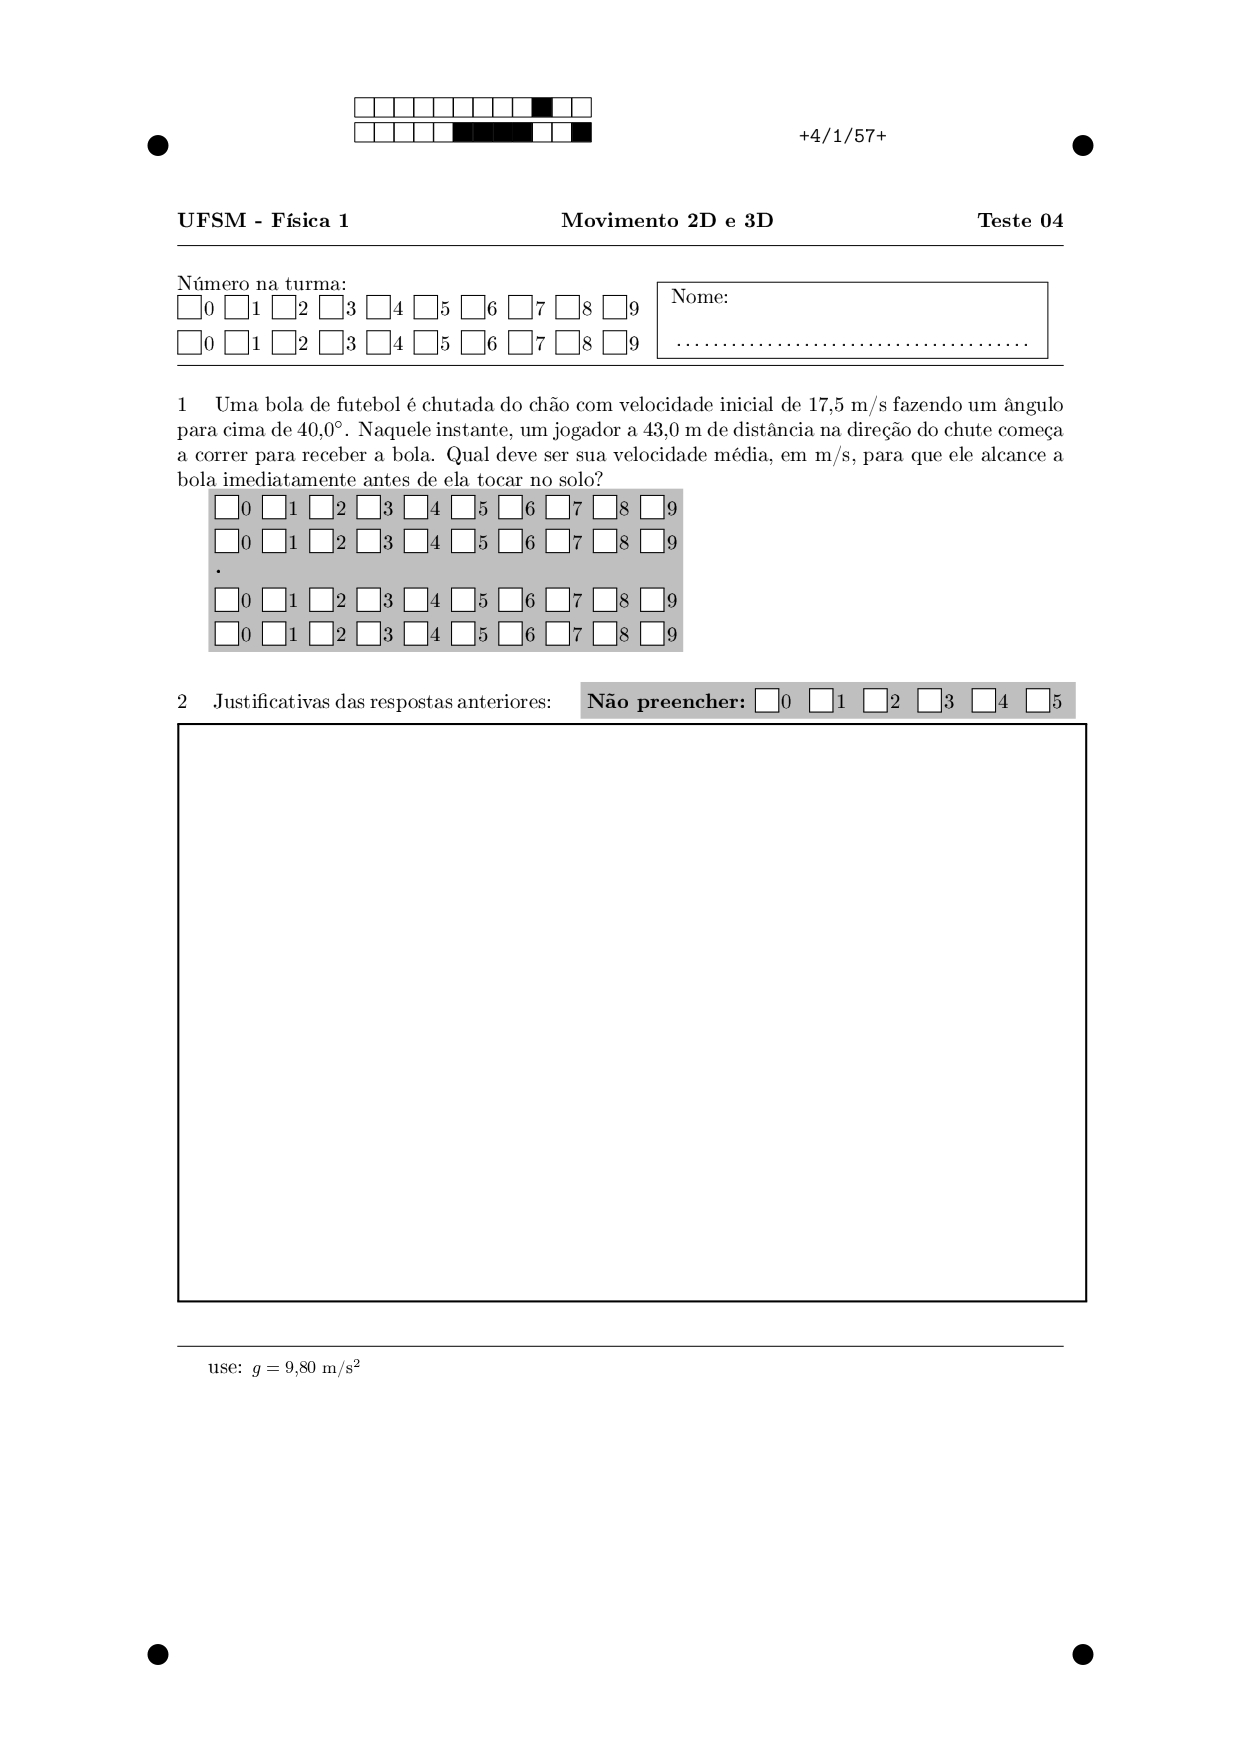
\includegraphics[scale=0.7]{fig/orp1q3_page-0004.jpg}
\end{figure}

\section{Atividade Síncrona 5} \label{ch:orp1e5}
\vspace*{\fill}
\begin{figure}[H]\centering
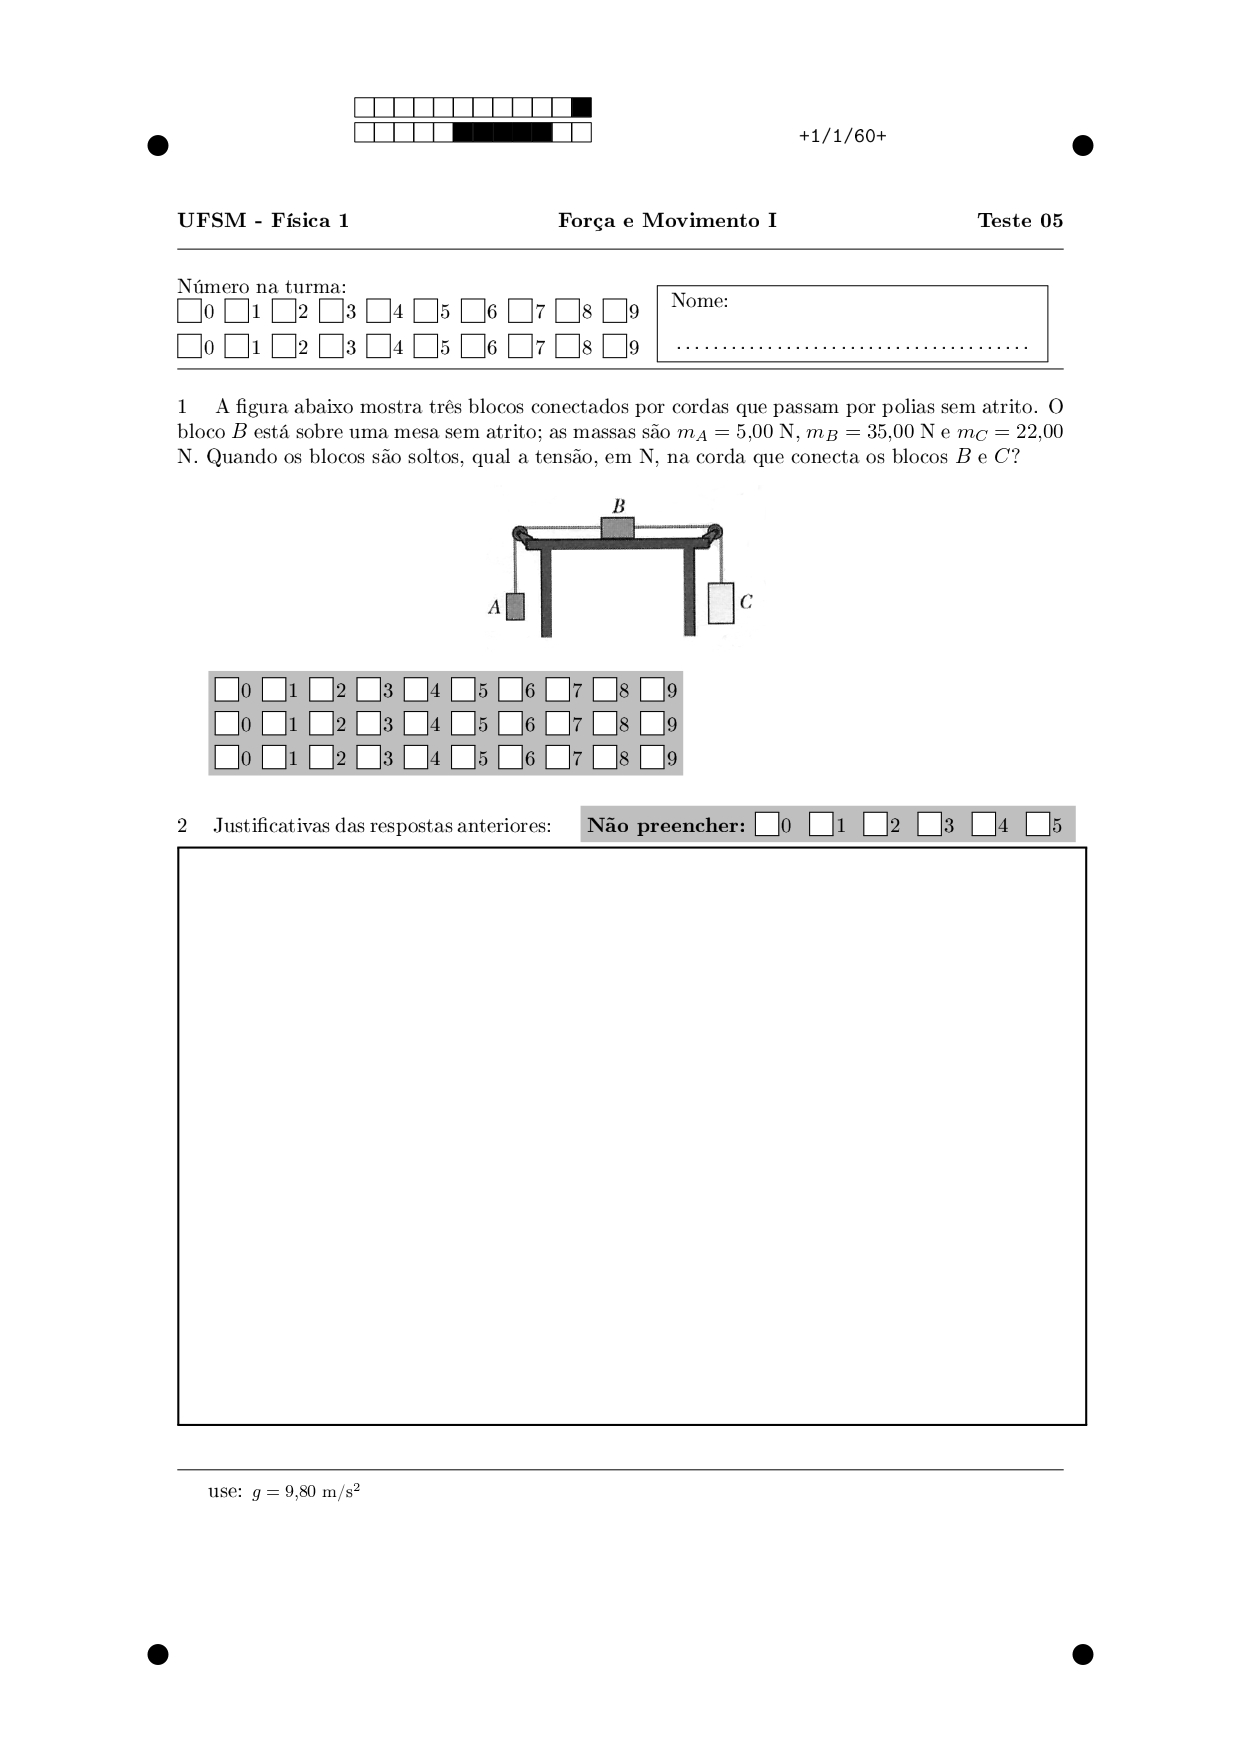
\includegraphics[scale=0.7]{fig/orp1q4_page-0001.jpg}
\end{figure}
\vspace*{\fill}
\begin{figure}[H]\centering
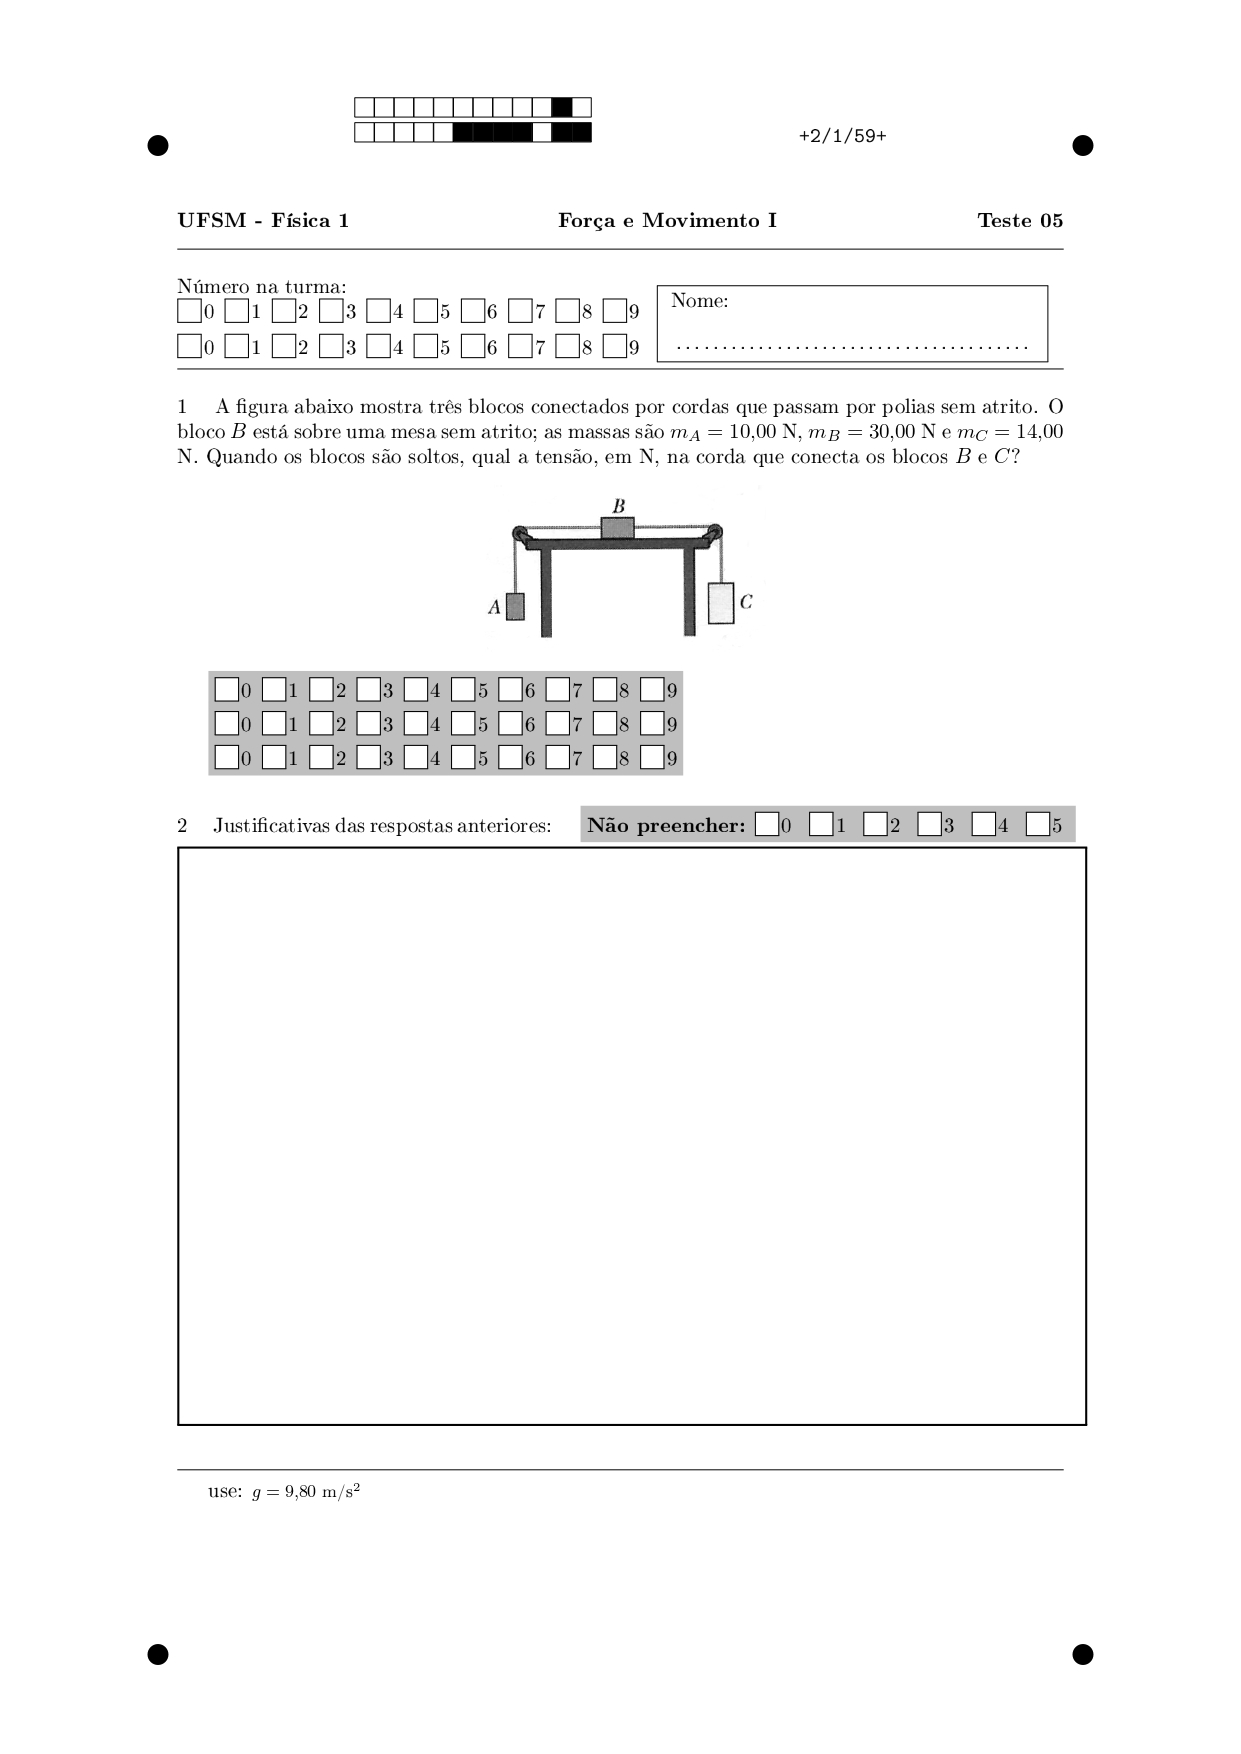
\includegraphics[scale=0.7]{fig/orp1q4_page-0002.jpg}
\end{figure}
\vspace*{\fill}
\begin{figure}[H]\centering
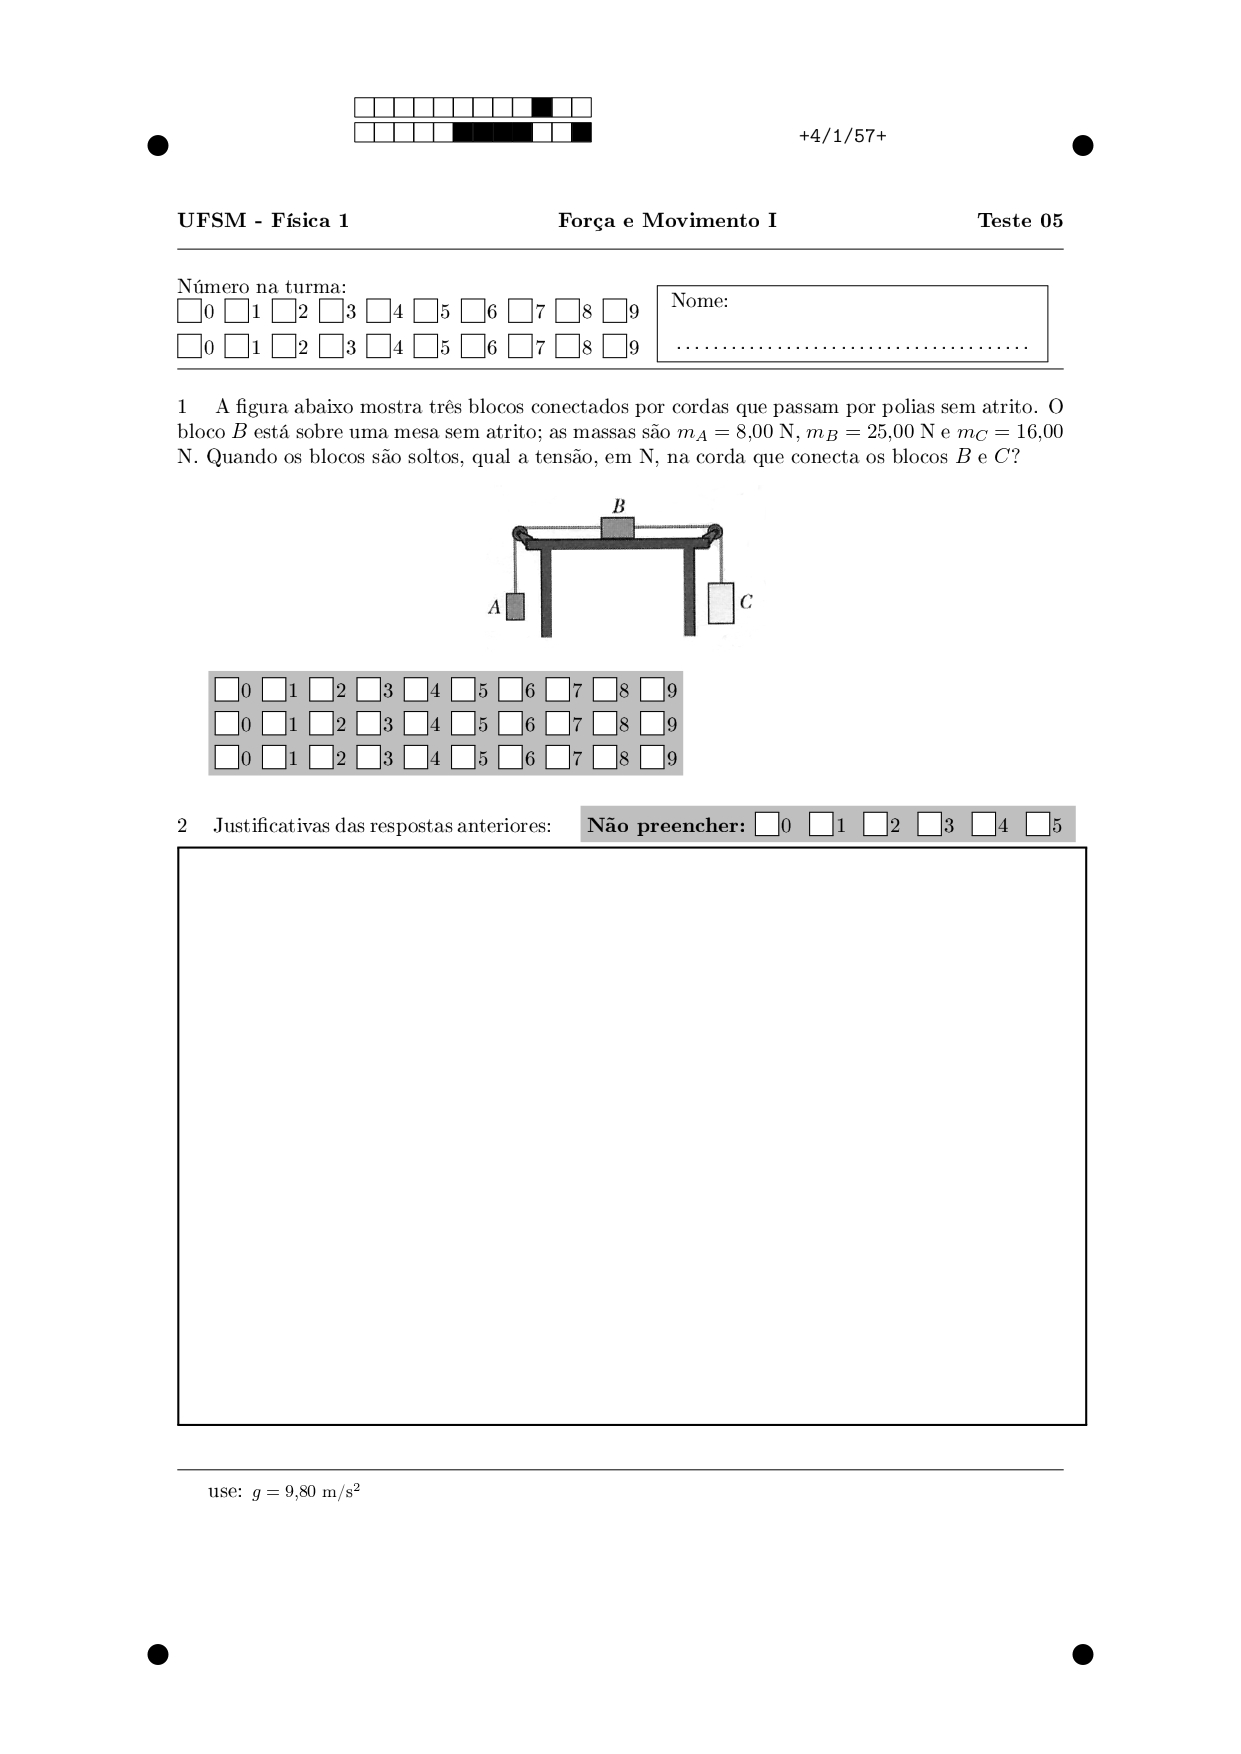
\includegraphics[scale=0.7]{fig/orp1q4_page-0004.jpg}
\end{figure}

\section{Atividade Síncrona Questão 6} \label{ch:orp1e6}
\vspace*{\fill}
\begin{figure}[H]\centering
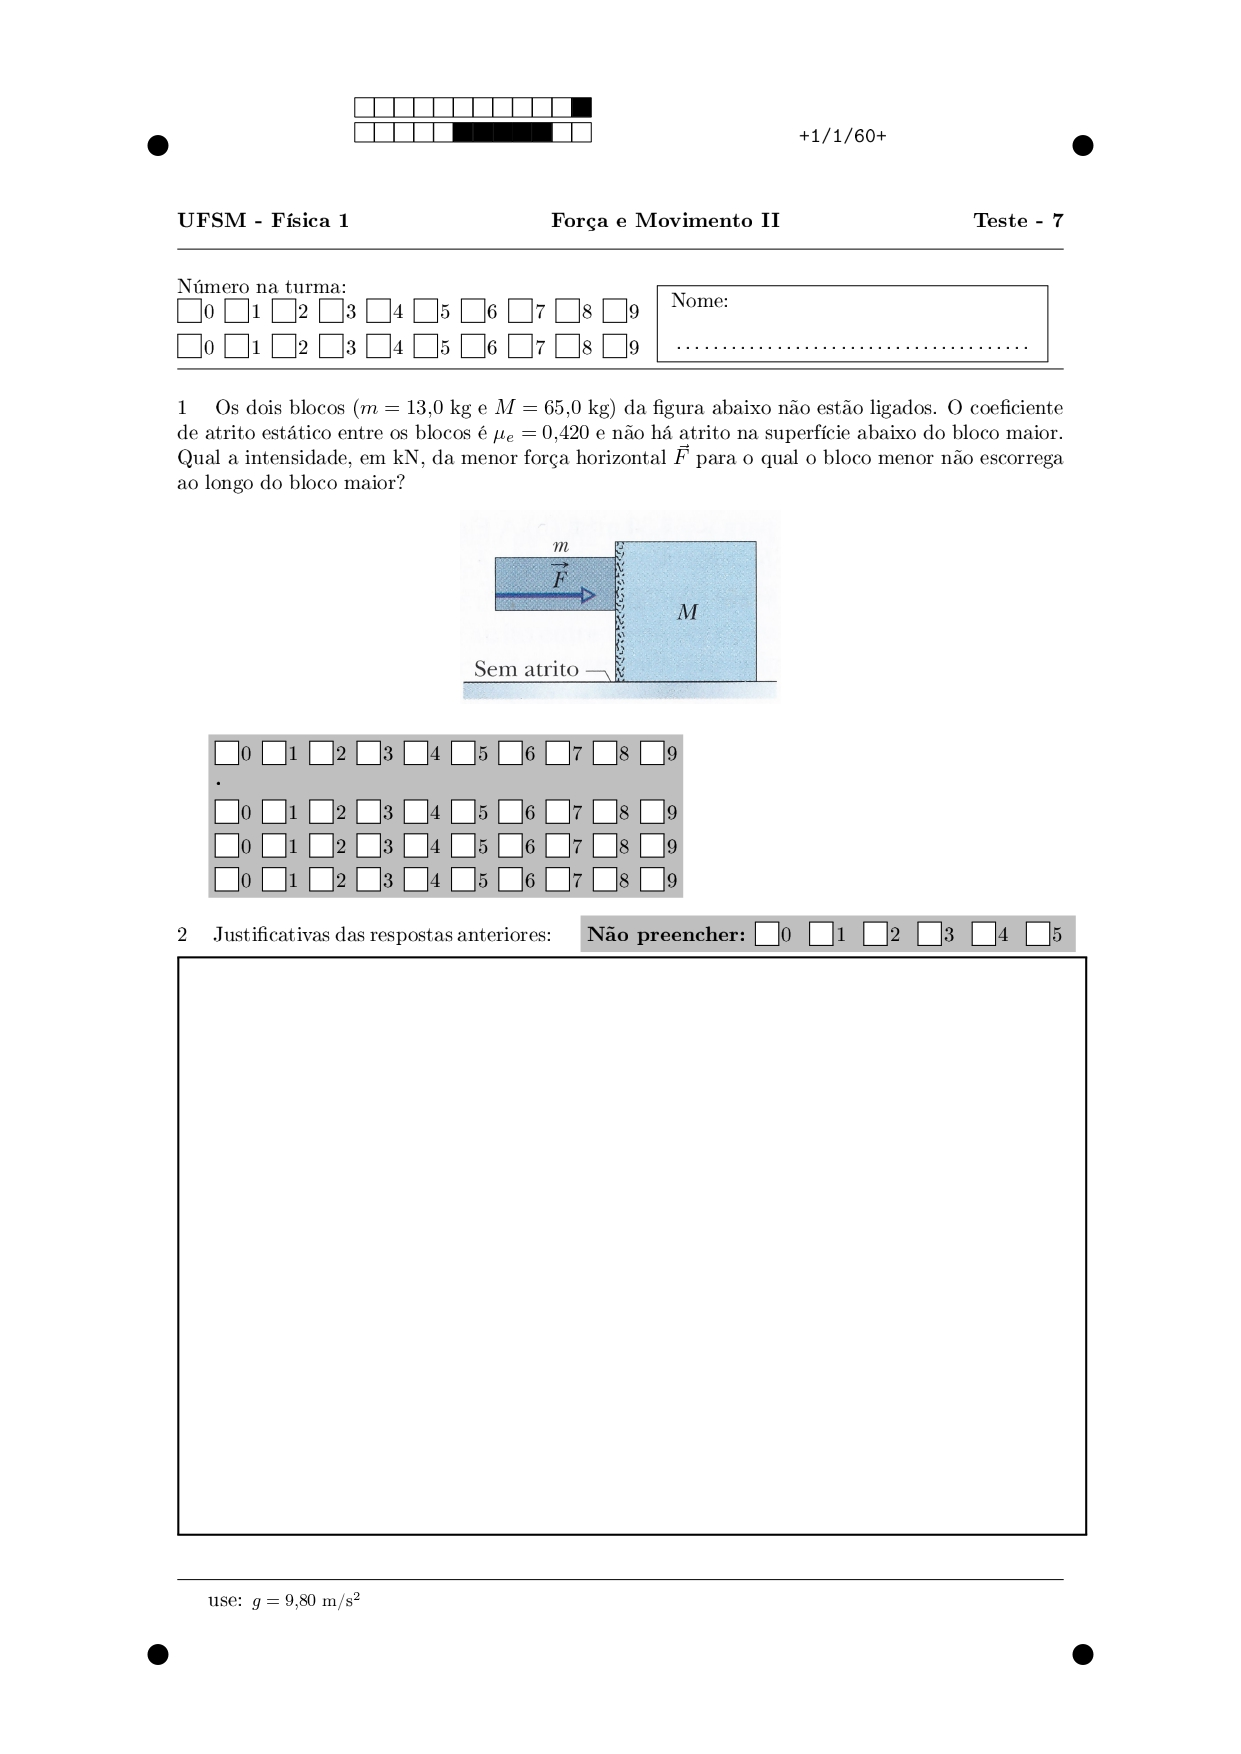
\includegraphics[scale=0.7]{fig/orp1q6_page-0001.jpg}
\end{figure}
\vspace*{\fill}
\begin{figure}[H]\centering
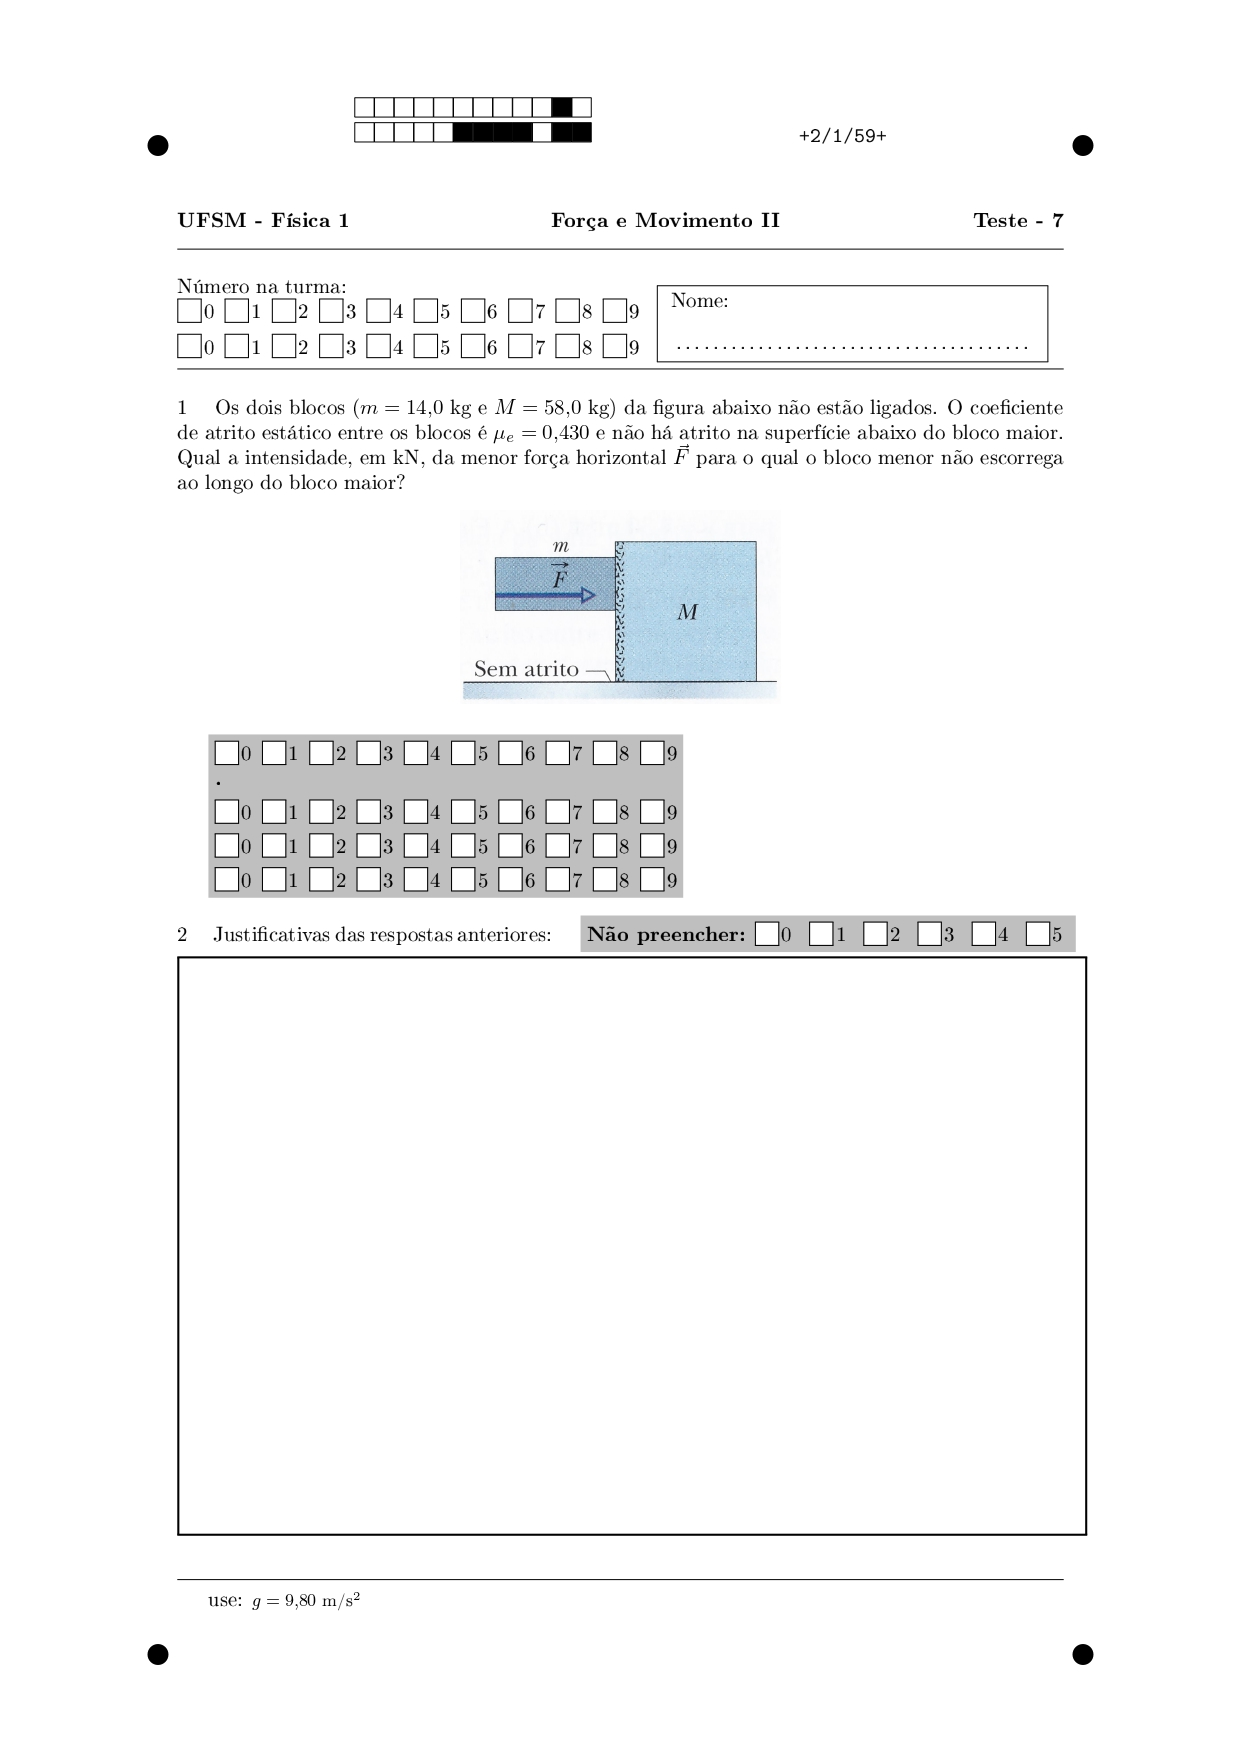
\includegraphics[scale=0.7]{fig/orp1q6_page-0002.jpg}
\end{figure}
\vspace*{\fill}
\begin{figure}[H]\centering
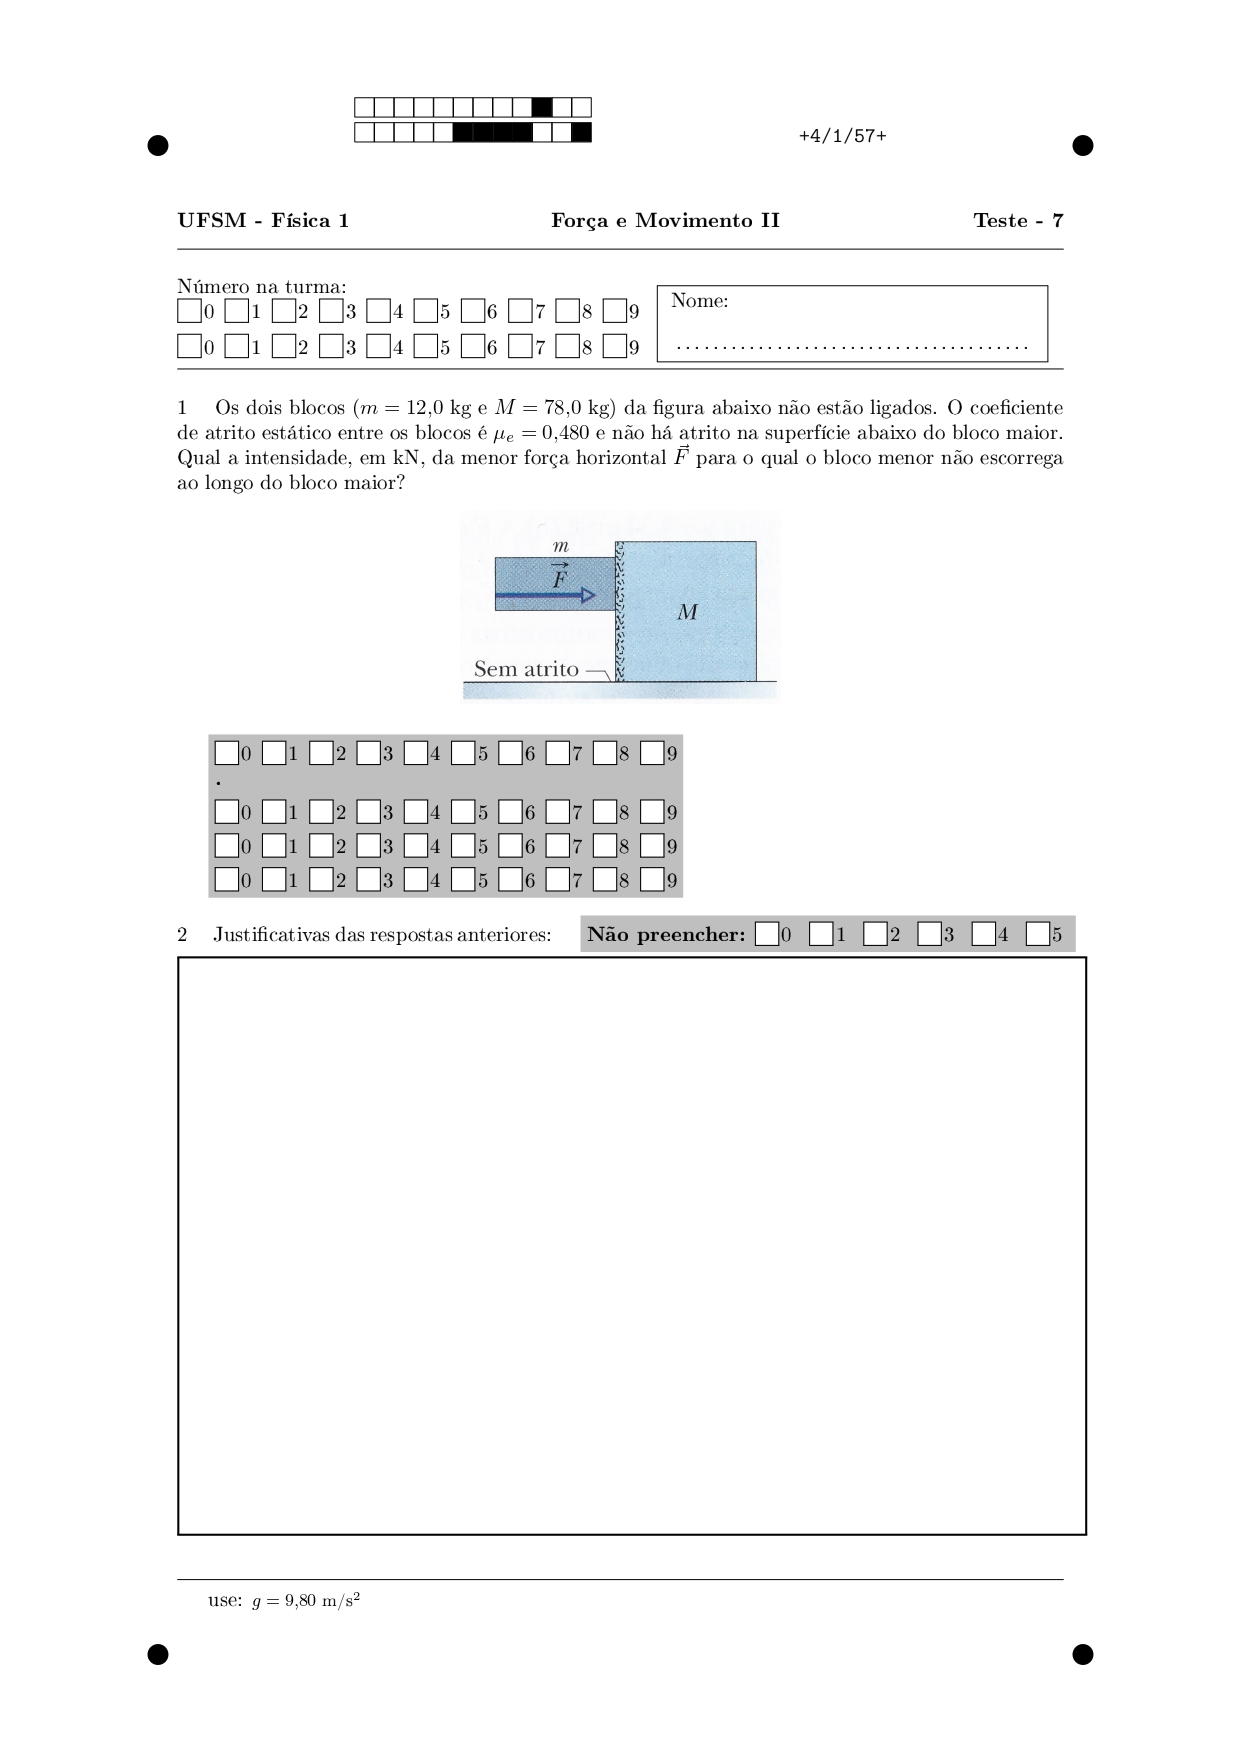
\includegraphics[scale=0.7]{fig/orp1q6_page-0004.jpg}
\end{figure}

\section{Atividade Síncrona 7} \label{ch:orp1e7}
\vspace*{\fill}
\begin{figure}[H]\centering
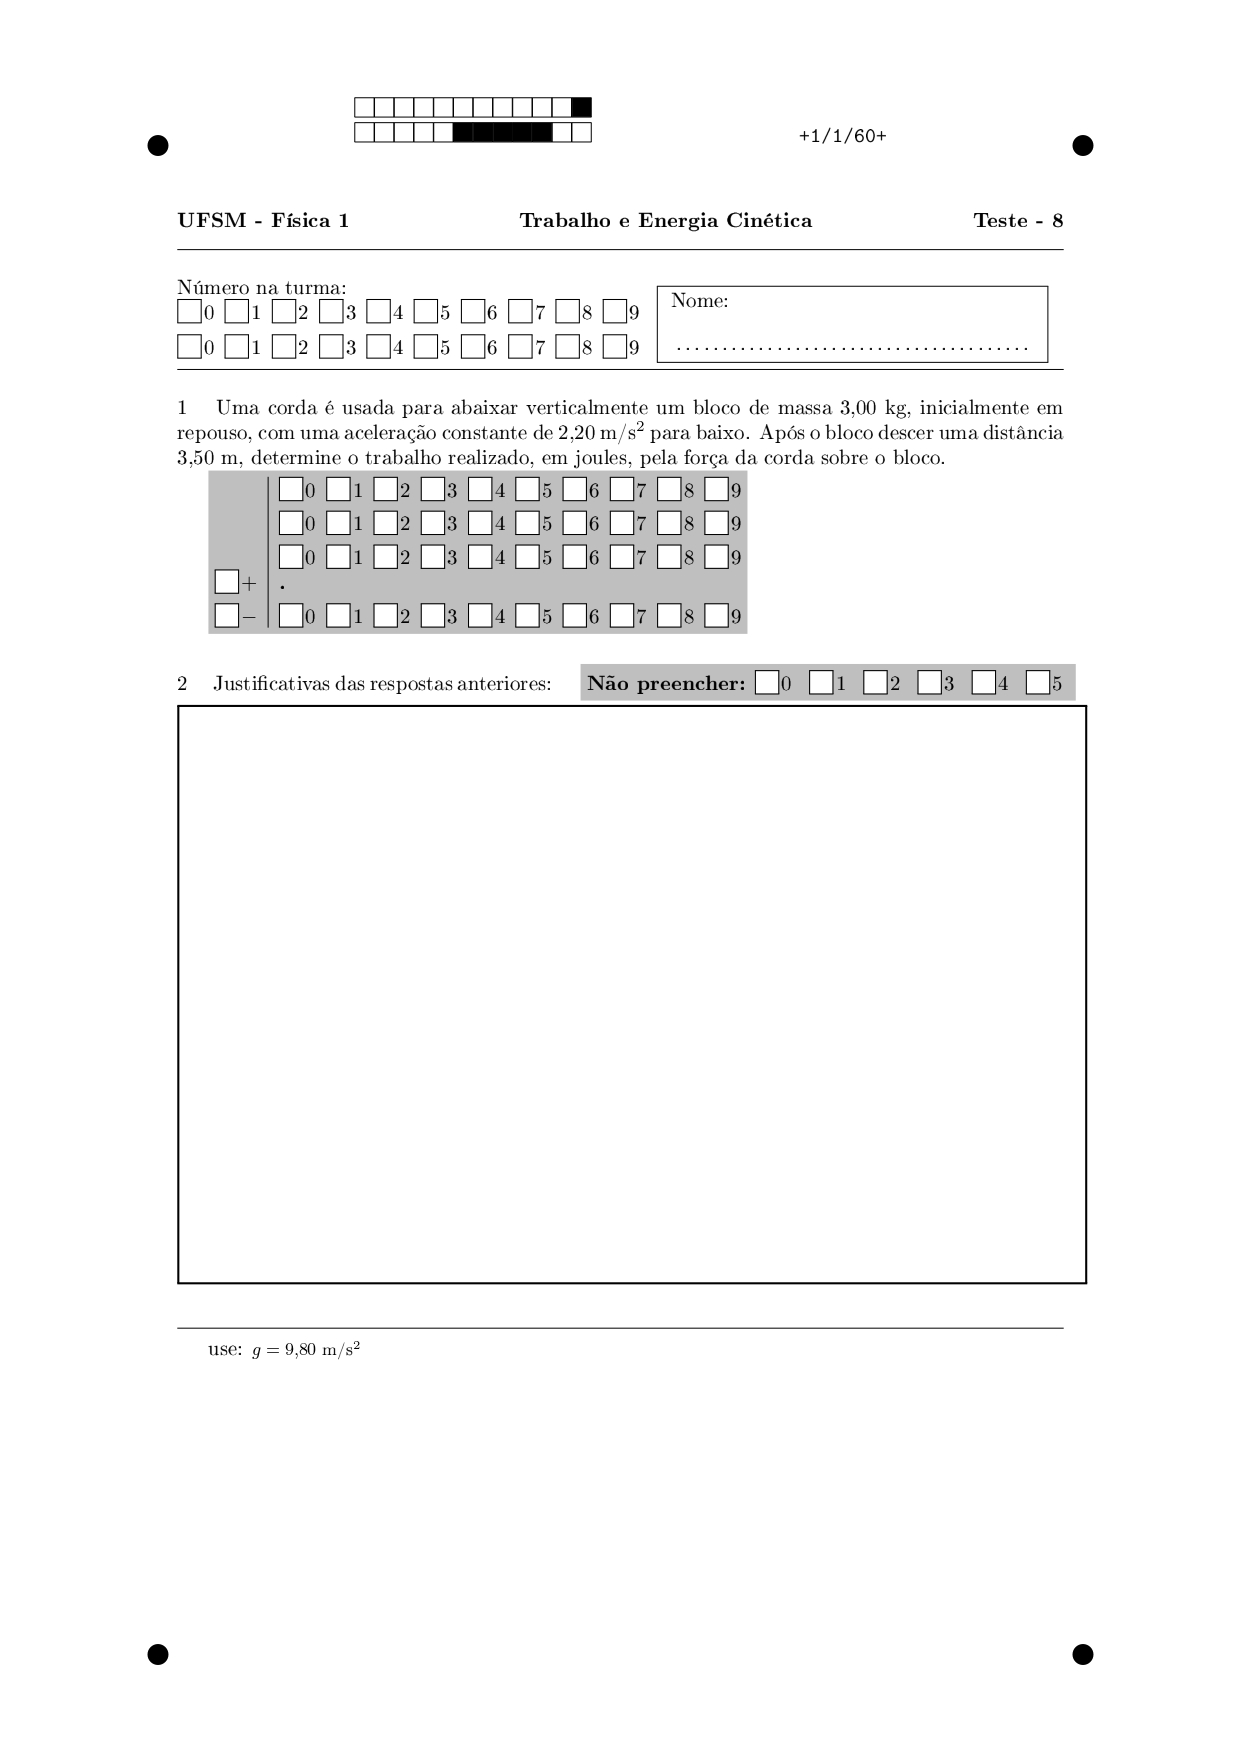
\includegraphics[scale=0.7]{fig/orp1q7_page-0001.jpg}
\end{figure}
\vspace*{\fill}
\begin{figure}[H]\centering
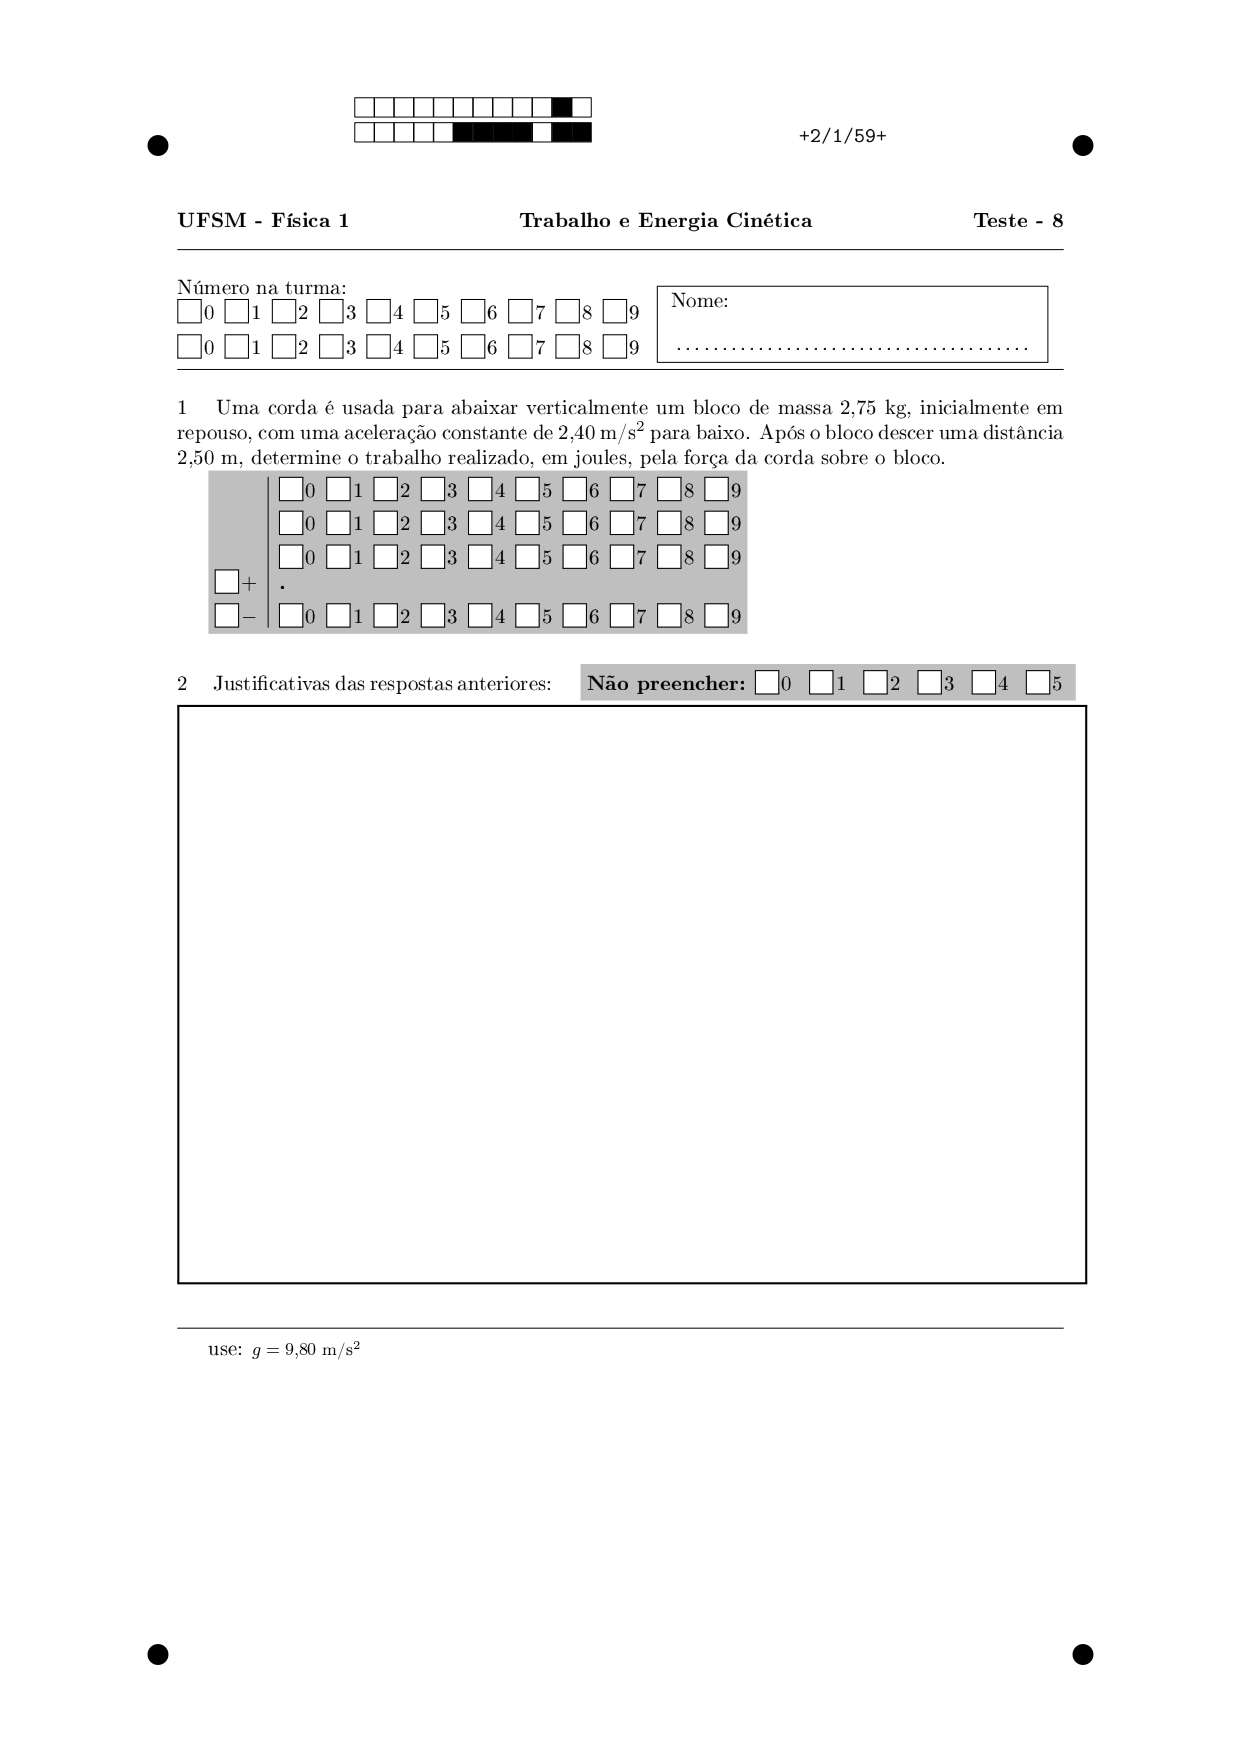
\includegraphics[scale=0.7]{fig/orp1q7_page-0002.jpg}
\end{figure}
\vspace*{\fill}
\begin{figure}[H]\centering
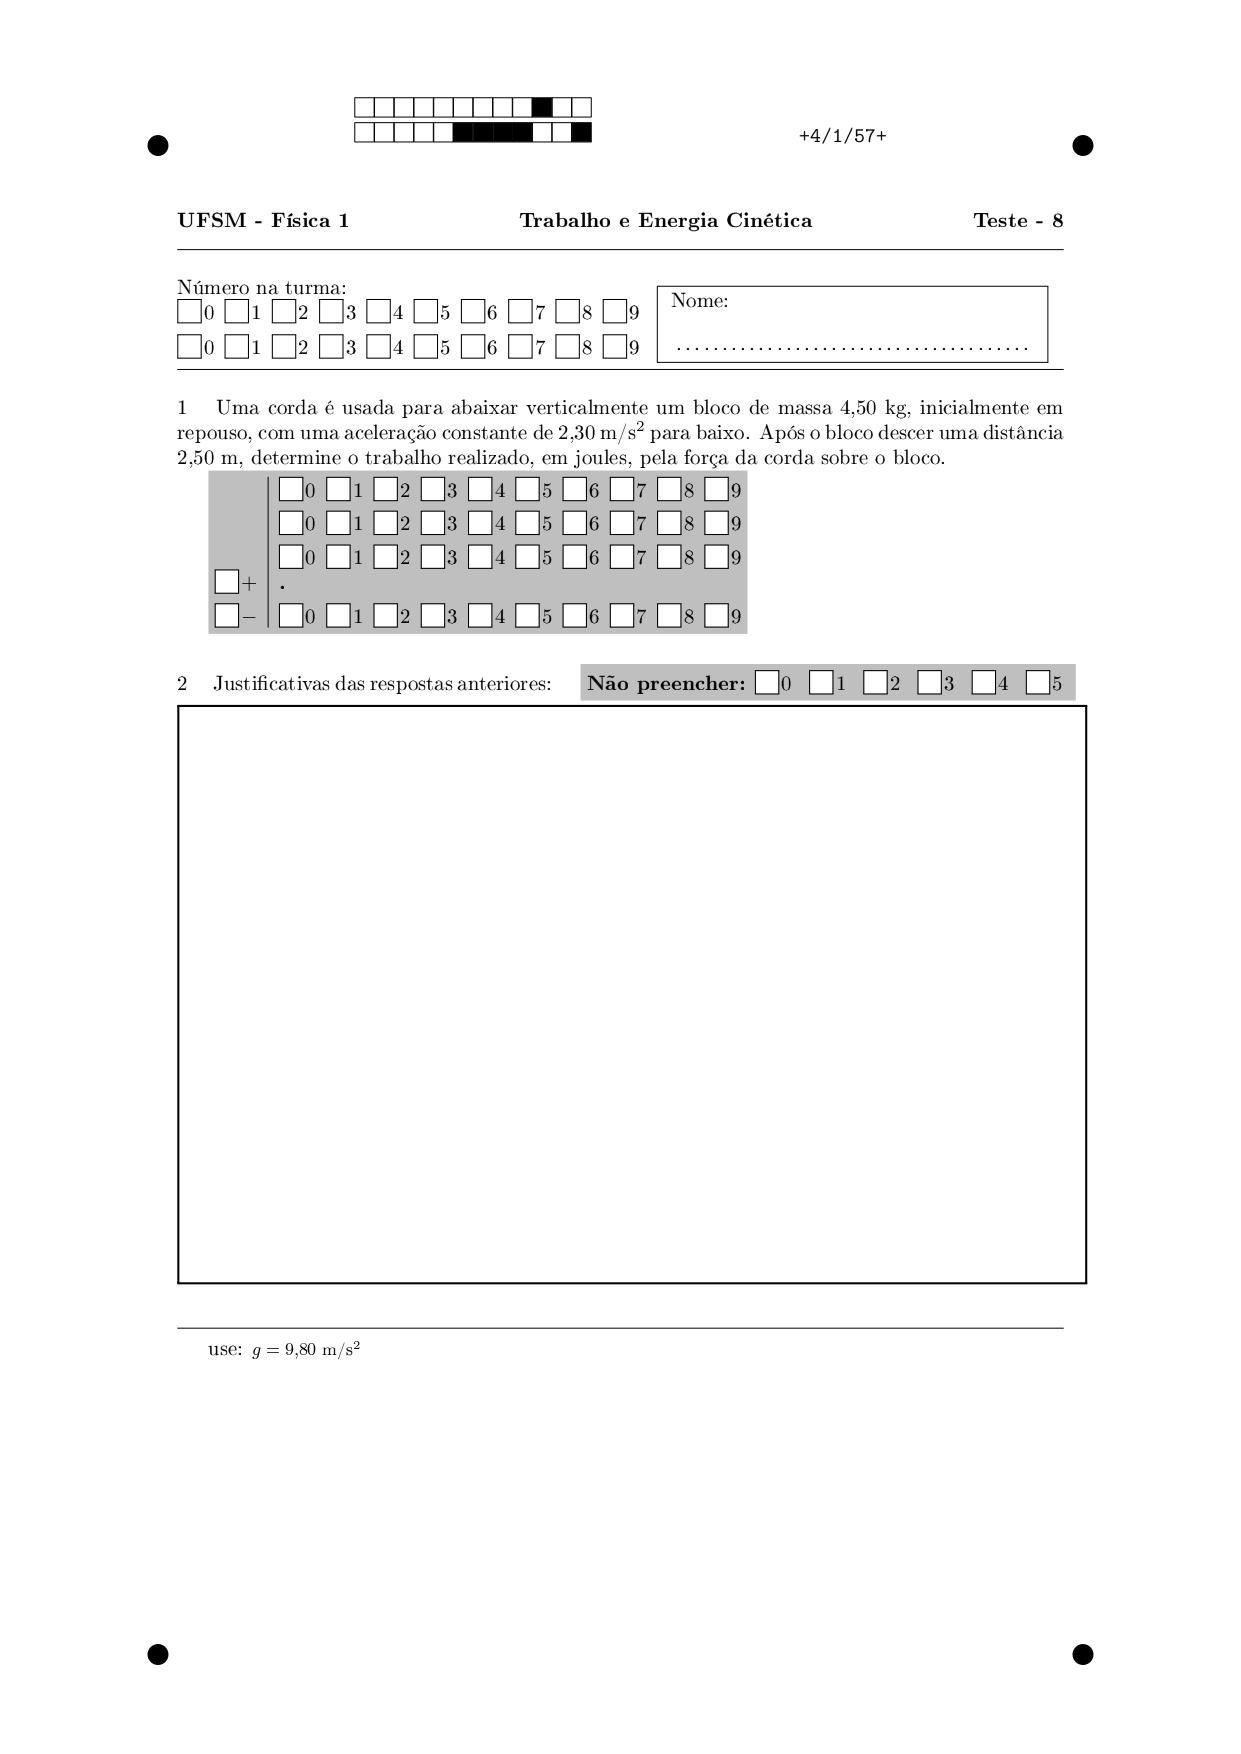
\includegraphics[scale=0.7]{fig/orp1q7_page-0004.jpg}
\end{figure}

\section{Atividade Síncrona 8} \label{ch:orp1e8}
\vspace*{\fill}
\begin{figure}[H]\centering
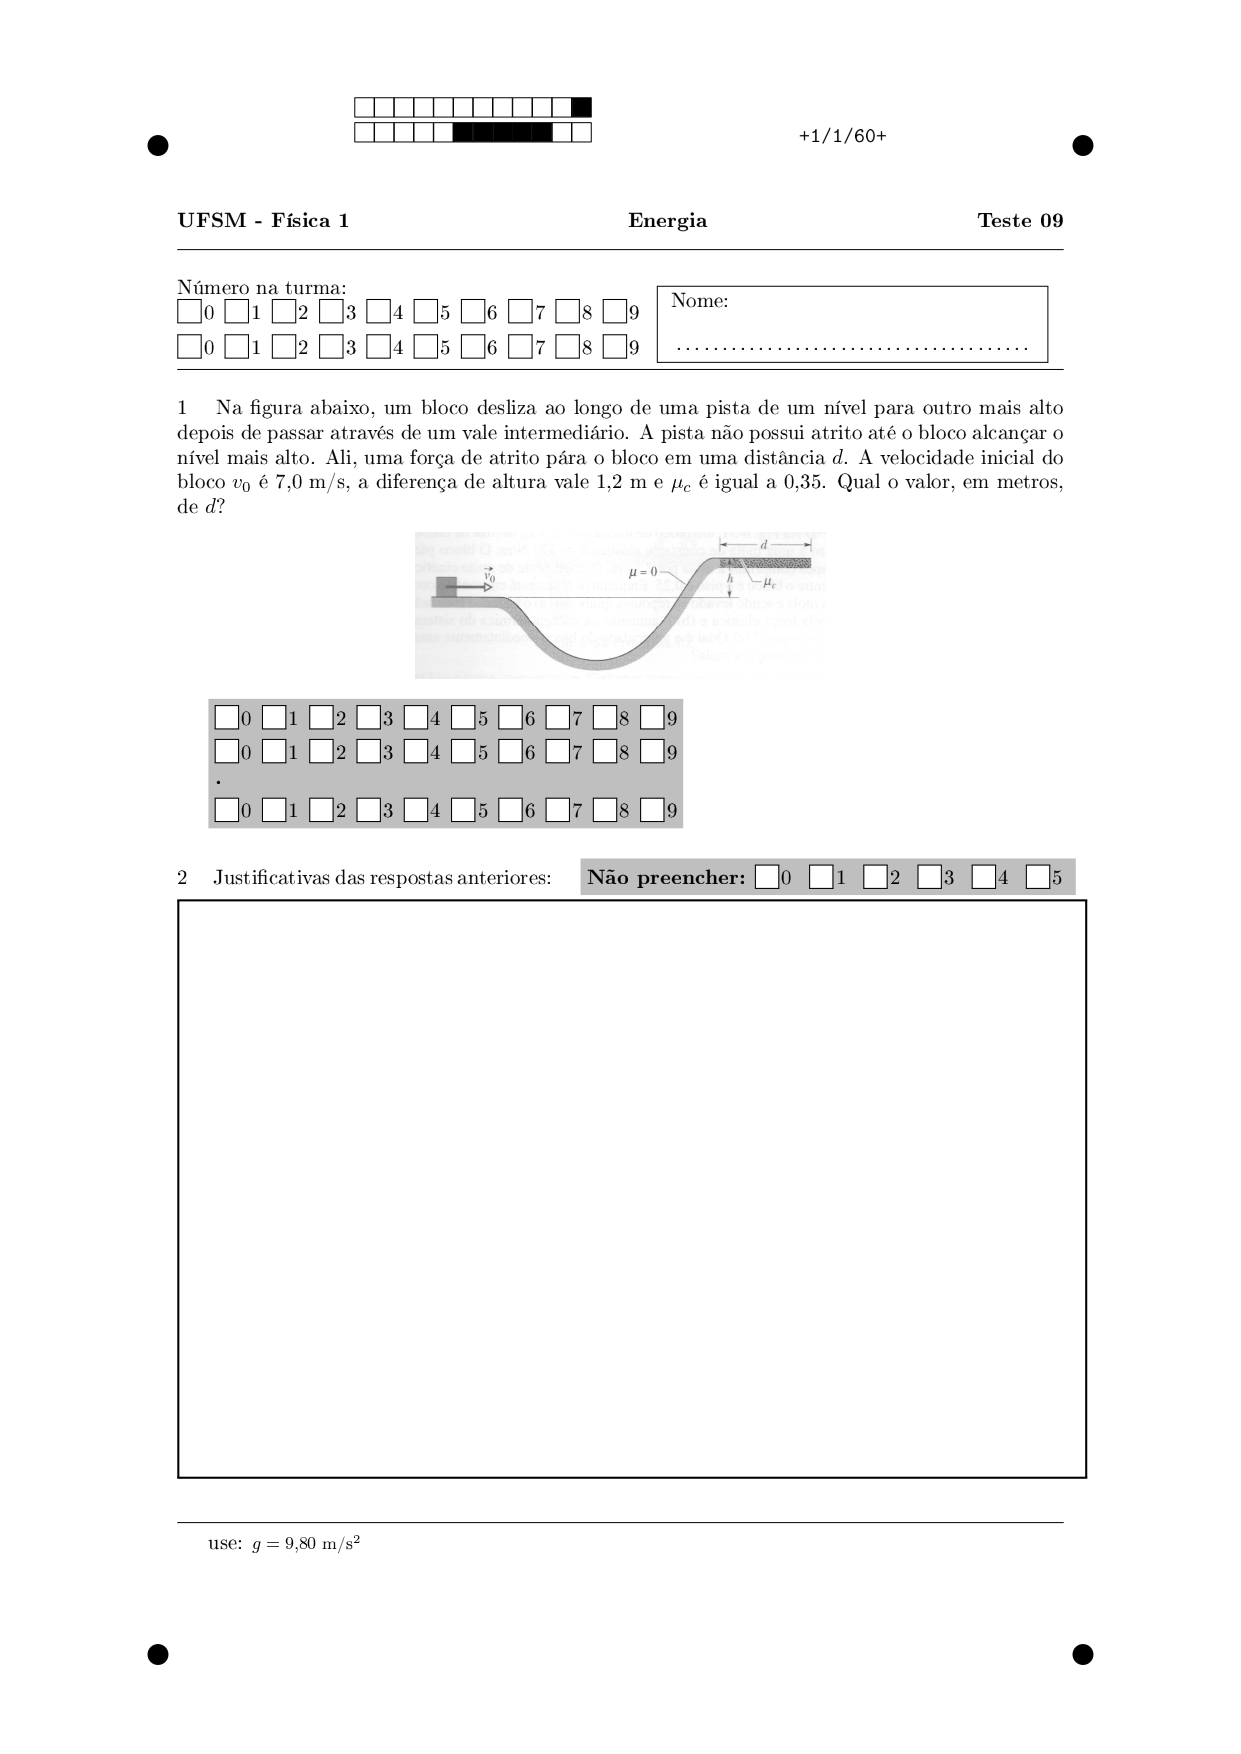
\includegraphics[scale=0.7]{fig/orp1q8_page-0001.jpg}
\end{figure}
\vspace*{\fill}
\begin{figure}[H]\centering
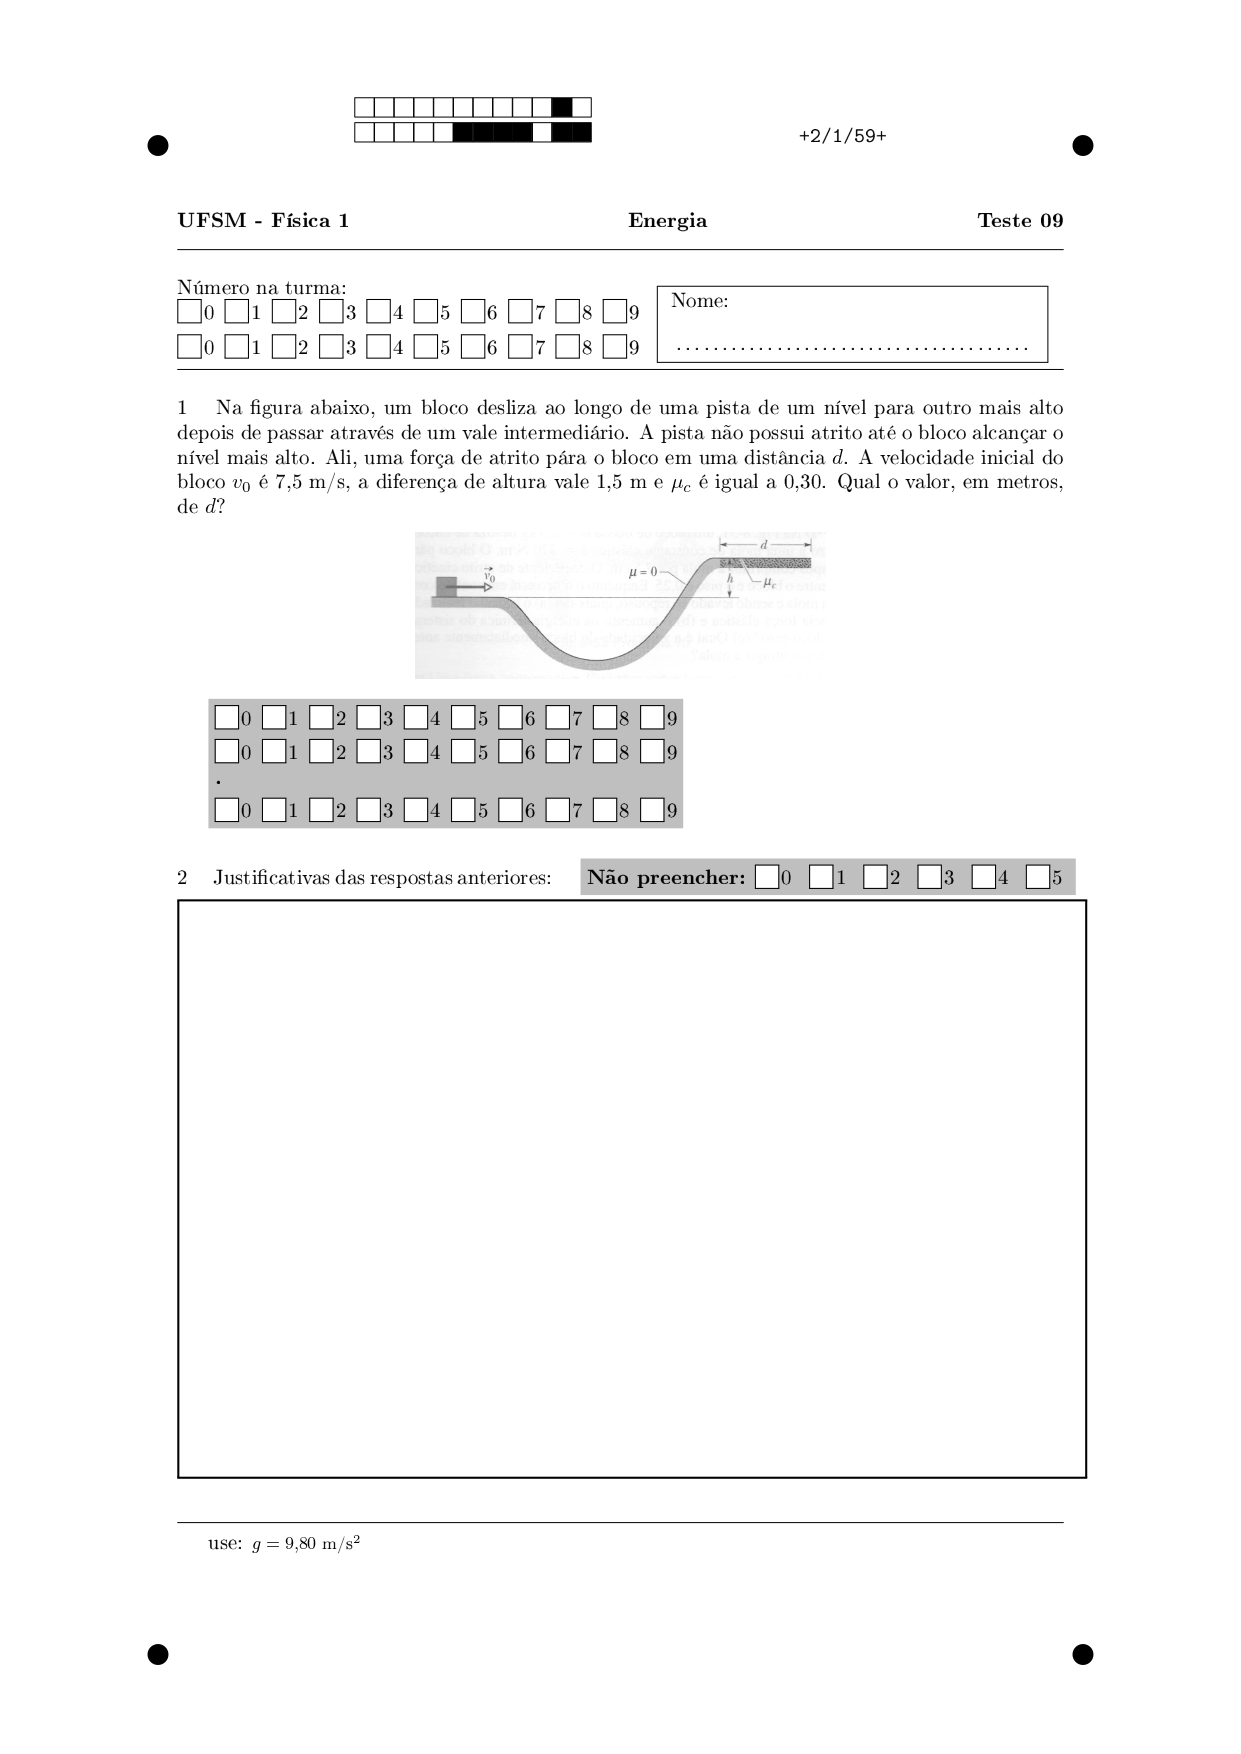
\includegraphics[scale=0.7]{fig/orp1q8_page-0002.jpg}
\end{figure}
\vspace*{\fill}
\begin{figure}[H]\centering
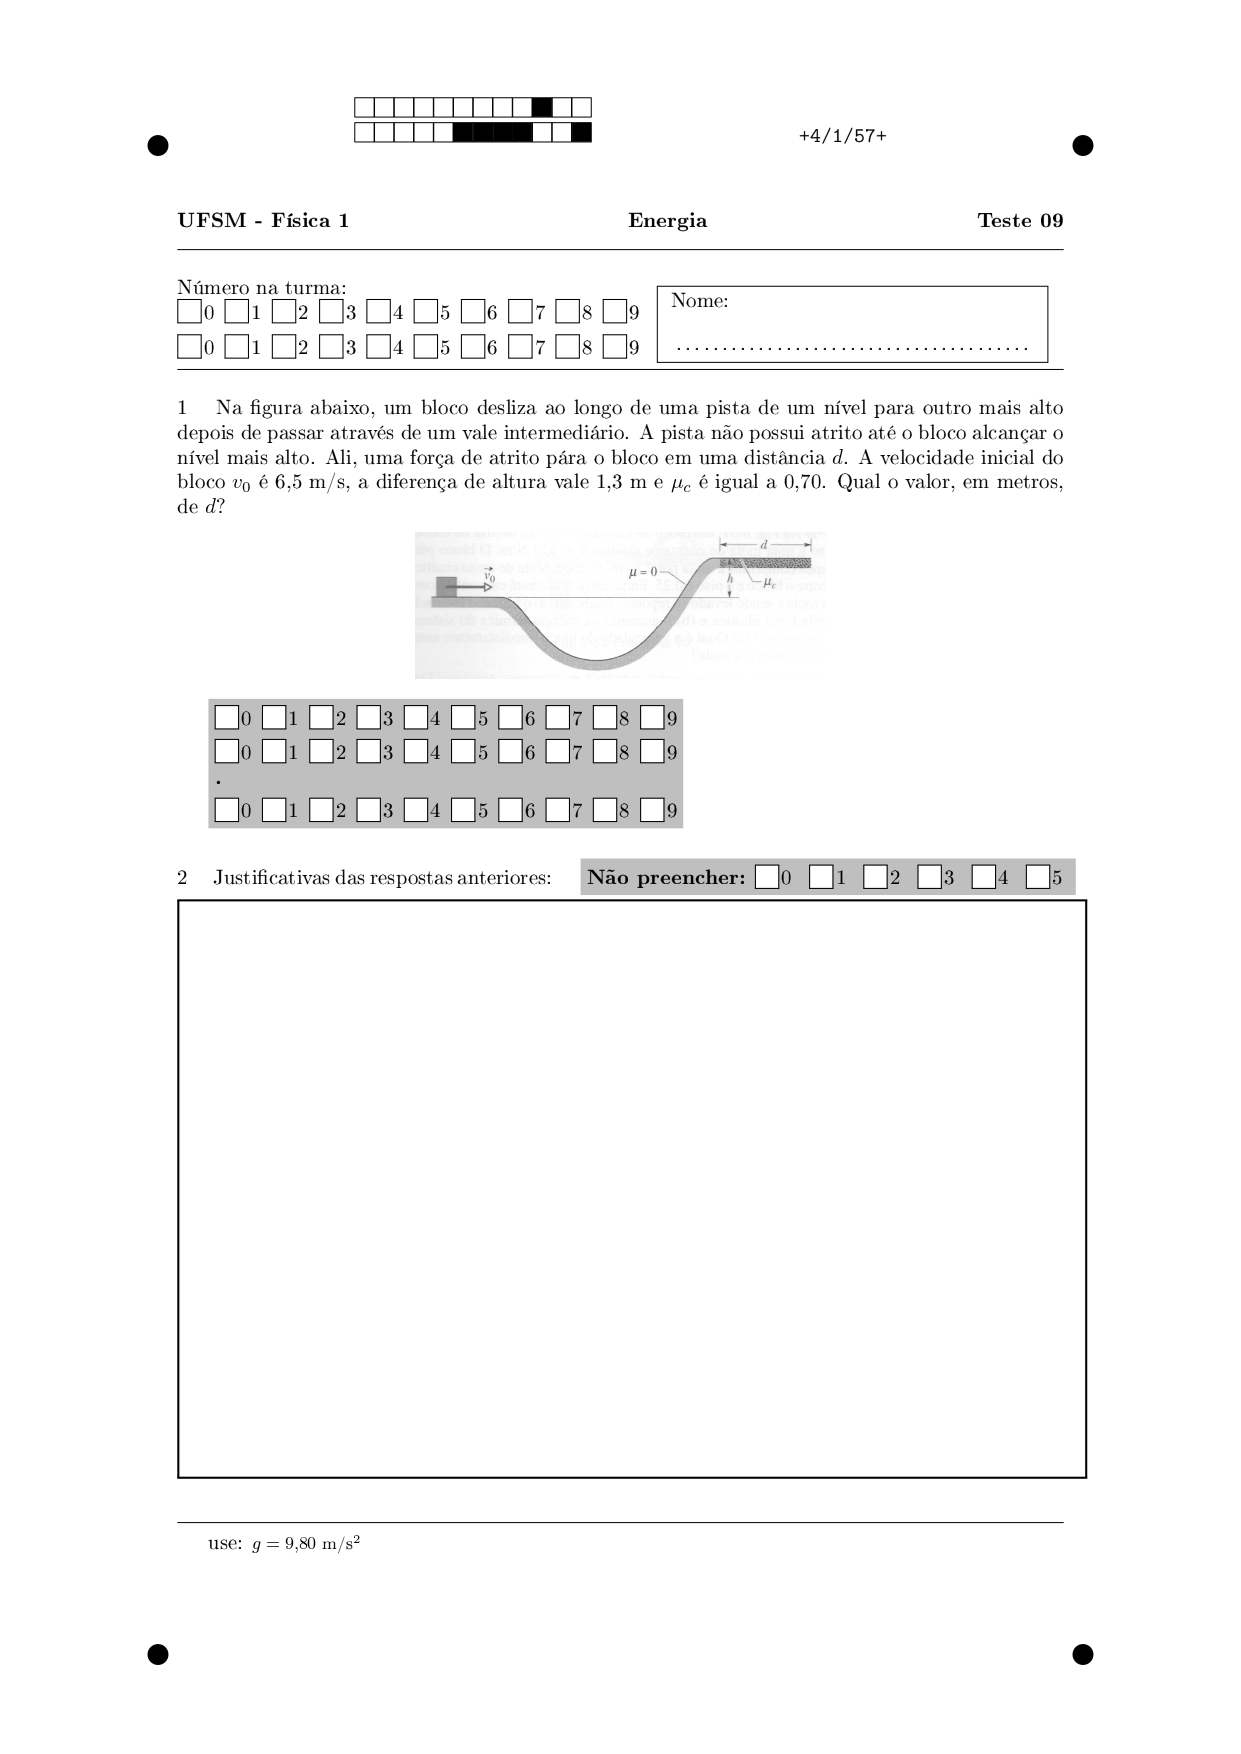
\includegraphics[scale=0.7]{fig/orp1q8_page-0004.jpg}
\end{figure}
\chapter{ORP 1 - Substitutivas} \label{ch:orp1subs}
\section*{Questão 1}
\textbf{\cite{Halliday2009}}
\begin{itemize}
    \item[(a)] Se a aceleração máxima que pode ser tolerada pelos passageiros de um metrô é $1,34$ $m/s^2$ e duas estações estão separadas por uma distância de $806$ $m$, qual é a velocidade máxima que o metrô pode alcançar entre as estações?
    \item[(b)] Qual o tempo de percurso?
    \item[(c)] Se o metrô pára por $20$ $s$ em cada estação, qual é a máxima velocidade escalar média do metrô de uma partida à próxima? 
\end{itemize}

\section*{Questão 2}

\textbf{\cite{Halliday2009}} Dois besouros correm em um deserto plano, partindo do mesmo ponto. O besouro 1 corre $0,50$ $m$ para leste e $0,80$ $m$ em uma direção $30^{\circ}$ ao norte do leste. O besouro 2 corre $1,6$ $m$ em uma direção $40^{\circ}$ ao leste do norte e depois corre em outra direção. Quais devem ser (a) o módulo e (b) o sentido da segunda corrida do segundo besouro para que ele termine na mesma posição final que o primeiro besouro?

\section*{Questão 3}

\textbf{\cite{Halliday2009}} Uma bola é lançada a partir do solo. Quando ela atinge ma altura de $9,1$ $m$ sua velocidade é $\vec{v} = (7,6 \hat{i} + 6,1 \hat{j})$ $m/s$, com $\hat{i}$ horizontal e $\hat{j}$ para cima. (a) Qual é a altura máxima atingida pela bola? (b) Qual é a distância horizontal coberta pela bola? Quais são (c) o módulo e (d) o ângulo (abaixo da horizontal) da velocidade da bola no instante em que ala atinge o solo? 

\section*{Questão 4}

\textbf{\cite{Halliday2009}} Na figura abaixo uma bola pe arremessada do alto de um edifício caindo $4,00$ $s$ de uma altura $h = 20,0$ $m$ acima da altura de lançamento. A trajetória da bola no final tem uma inclinação $\theta = 60^{\circ}$ em relação à horizontal. (a) Determine a distância horizontal $d$ coberta pela bola. Quais são (b) o módulo e (c) o ângulo (em relação à horizontal) da velocidade inicial da bola?
\begin{figure}[ht]
\begin{center}
\caption*{Esboço Substituutiva Questão 4.}
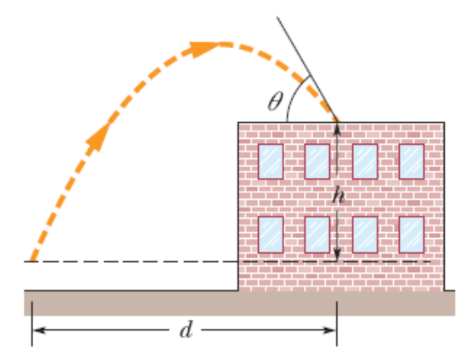
\includegraphics[width=0.4\textwidth]{fig/orp1subs5.png}
\label{fig:ORP1s4}
\caption*{Fonte: \citeonline{Halliday2009}}
\end{center}
\end{figure}

\section*{Questão 5}

\textbf{\cite{Halliday2009}} A figura abaixo mostra uma caixa de massa $m_2 = 1,0$ $kg$ em um plano inclinado sem atrito de ãngulo $\theta = 30^{\circ}$, que está ligada por uma corda, de massa desprezível, a uma outra caixa de massa $m_1 = 3,0$ $kg$ em uma superfície horizontal e sem atrito. A polia não tem atrito e sua massa é desprezível.
\begin{itemize}
    \item[(a)] Se o módulo da força horizontal $\vec{F}$ é $2,3$ $N$, qual é a tração da corda?
    \item[(b)] Qual é o maior valor que o módulo de $\vec{F_2}$ pode ter sem que a corda fique frouxa?
\end{itemize}

\begin{figure}[ht]
\begin{center}
\caption*{Esboço Substituutiva Questão 5.}
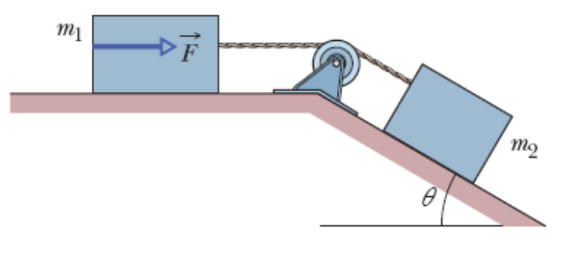
\includegraphics[width=0.4\textwidth]{fig/orp1s5real.png}
\label{fig:ORP1s5}
\caption*{Fonte: \citeonline{Halliday2009}}
\end{center}
\end{figure}

\section*{Questão 6}

\textbf{(\cite{TiplerMosca2006}/Adaptado)} Um bloco de $2,0$ $kg$ é colocado sobre um bloco de $4,0$ $kg$ que está sobre uma mesa sem atrito (ver figura abaixo). Os coefcientes de  atrito entre os blocos são ${\mu}_e = 0,30$ e ${\mu}_c = 0,20$. (a) Qual é a máxima força horizontal $F$ que pode ser aplicada ao bloco de $4,0$ $kg$ se o bloco de $2,0$ $kg$ não deve deslizar? (b) se $F$ tem metade deste valor, encontre a aceleração de cada bloco e a força de atrito atuando sobre cada bloco. (c) Se $F$ tem o dobro do valor encontrado em (a), encontre a aceleração de cada bloco.

\begin{figure}[ht]
\begin{center}
\caption*{Esboço Substituutiva Questão 6.}
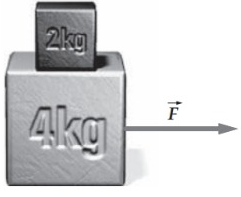
\includegraphics[width=0.4\textwidth]{fig/orp1s6.png}
\label{fig:ORP1s6}
\caption*{Fonte: \citeonline{TiplerMosca2006}}
\end{center}
\end{figure}

\section*{Questão 7}

\textbf{\cite{TiplerMosca2006}} Um bloco de $6,0$ $kg$ escorrega $1,5$ $m$ abaixo sobre um plano inclinado sem atrito que forma um ângulo de $60^{\circ}$ com a horizontal. (a) Desenhe o diagrama de corpo livre para o bloco e encontre o trabalho realizado por cada força, enquanto o bloco escorrega $1n5$ $m$ (medidos ao longo do plano inclinado). (b) Qual é o trabalho total realizado sobre o bloco? (c) Qual é a rapidez do bloco após ter escorregado $1,5$ $m$, se ele parte do repouso? (d) Qual é a sua rapidez, após $1,5$ $m$, se ele parte com uma rapidez inicial de $2,0$ $m/s$?

\section*{Questão 8}

\textbf{\cite{TiplerMosca2006}} Um carrinho de montanha-russa está se movendo com rapidez $v_0$ no início do percurso, quando desce um vale de $5,0$ $m$ e depois sobe até o topo de uma elevação, $4,5$ $m$ acima do início do percurso. Desconsidere o atrito e a resistência do ar. (a) Qual é a menor rapidez $v_0$ necessária para que o carrinho ultrapasse o topo da elevação? (b) Esta rapidez pode ser alterada modificando-se a profundidade do vale, para que o carrinho adquira mais rapidez lá embaixo? Explique.

\chapter{QUESTIONÁRIO ORP1} \label{ch:questORP1}
\begin{center}
    \textbf{Questionário de fim de Semestre}

    
    Curso de Engenharia Civil - UFSM
\end{center}

Marque o número que corresponde ao critério que melhor corresponde à sua opinião em relação às perguntas a seguir:

\begin{itemize}
    \item Você acredita que as atividades avaliativas, da forma como foram apicadas, estão colaboraram para seu processo de aprendizagem?

\begin{minipage}{\linewidth}
\centering
\begin{tabular}{|c|c|c|c|c|}
\hline
\textbf{1} & \textbf{2} & \textbf{3} & \textbf{4} & \textbf{5} \\
\hline
Discordo totalmente & \phantom{aaaaaaaa} & \phantom{aaaaaaaa} & \phantom{aaaaaaaa} & Concordo totalmente \\
\hline
\end{tabular}
\end{minipage}

    \item Na sua opinião, os problemas presentes nos Testes de um grau de dificuldade aceitável para uma tarefa avaliativa?
    
\begin{minipage}{\linewidth}
\centering
\begin{tabular}{|c|c|c|c|c|}
\hline
\textbf{1} & \textbf{2} & \textbf{3} & \textbf{4} & \textbf{5} \\
\hline
Discordo totalmente & \phantom{aaaaaaaa} & \phantom{aaaaaaaa} & \phantom{aaaaaaaa} & Concordo totalmente \\
\hline
\end{tabular}
\end{minipage}

    \item Sobre os Testes Substitutivos, você concorda que a sua aplicação contribui para a sua aprendizagem?

\begin{minipage}{\linewidth}
\centering
\begin{tabular}{|c|c|c|c|c|}
\hline
\textbf{1} & \textbf{2} & \textbf{3} & \textbf{4} & \textbf{5} \\
\hline
Discordo totalmente & \phantom{aaaaaaaa} & \phantom{aaaaaaaa} & \phantom{aaaaaaaa} & Concordo totalmente \\
\hline
\end{tabular}
\end{minipage}

    \item Você acredita que os problemas presentes nos Teste Substitutivos tem o mesmo grau de dificuldade que os presentes nos Testes Síncronos?

\begin{minipage}{\linewidth}
\centering
\begin{tabular}{|c|c|c|c|c|}
\hline
\textbf{1} & \textbf{2} & \textbf{3} & \textbf{4} & \textbf{5} \\
\hline
Discordo totalmente & \phantom{aaaaaaaa} & \phantom{aaaaaaaa} & \phantom{aaaaaaaa} & Concordo totalmente \\
\hline
\end{tabular}
\end{minipage}

    \item Você tem tido dificuldades na hora de resolver as Listas de Exercícios?

\begin{minipage}{\linewidth}
\centering
\begin{tabular}{|c|c|c|c|c|}
\hline
\textbf{1} & \textbf{2} & \textbf{3} & \textbf{4} & \textbf{5} \\
\hline
Discordo totalmente & \phantom{aaaaaaaa} & \phantom{aaaaaaaa} & \phantom{aaaaaaaa} & Concordo totalmente \\
\hline
\end{tabular}
\end{minipage}

    \item  Você tem tido dificuldade para resolver os Testes Síncronos?

\begin{minipage}{\linewidth}
\centering
\begin{tabular}{|c|c|c|c|c|}
\hline
\textbf{1} & \textbf{2} & \textbf{3} & \textbf{4} & \textbf{5} \\
\hline
Discordo totalmente & \phantom{aaaaaaaa} & \phantom{aaaaaaaa} & \phantom{aaaaaaaa} & Concordo totalmente \\
\hline
\end{tabular}
\end{minipage}

    \item  Você tem tido dificuldades de resolver os Testes Substitutivos? 
    
\begin{minipage}{\linewidth}
\centering
\begin{tabular}{|c|c|c|c|c|}
\hline
\textbf{1} & \textbf{2} & \textbf{3} & \textbf{4} & \textbf{5} \\
\hline
Discordo totalmente & \phantom{aaaaaaaa} & \phantom{aaaaaaaa} & \phantom{aaaaaaaa} & Concordo totalmente \\
\hline
\end{tabular}
\end{minipage}

    \item Você tem procurado ajuda para estudar e tirar dúvidas, seja do professor ou de outras fontes?

\begin{minipage}{\linewidth}
\centering
\begin{tabular}{|c|c|c|c|c|}
\hline
\textbf{1} & \textbf{2} & \textbf{3} & \textbf{4} & \textbf{5} \\
\hline
Discordo totalmente & \phantom{aaaaaaaa} & \phantom{aaaaaaaa} & \phantom{aaaaaaaa} & Concordo totalmente \\
\hline
\end{tabular}
\end{minipage}

    \item Você tem precisado de consulta para a realização dos Testes Síncronos e/ou Substitutivos?

\begin{minipage}{\linewidth}
\centering
\begin{tabular}{|c|c|c|c|c|}
\hline
\textbf{1} & \textbf{2} & \textbf{3} & \textbf{4} & \textbf{5} \\
\hline
Discordo totalmente & \phantom{aaaaaaaa} & \phantom{aaaaaaaa} & \phantom{aaaaaaaa} & Concordo totalmente \\
\hline
\end{tabular}
\end{minipage}
\end{itemize}



\begin{table}[ht]
\captionsetup{justification=centering, labelsep=newline} % Centralize a legenda horizontalmente e adicione uma nova linha após o rótulo
\begin{tabularx}{\linewidth}{|>{\centering\arraybackslash}X|}
\hline
\textbf{Expresse livremente sua opinião sobre os Testes Síncronos e Substitutivos} \\
\hline
\rule{\dimexpr\linewidth-2\tabcolsep}{0.4pt} \\
\rule{\dimexpr\linewidth-2\tabcolsep}{0.4pt} \\
\rule{\dimexpr\linewidth-2\tabcolsep}{0.4pt} \\
\rule{\dimexpr\linewidth-2\tabcolsep}{0.4pt} \\
\rule{\dimexpr\linewidth-2\tabcolsep}{0.4pt} \\
\hline
\end{tabularx}

\end{table}


\begin{table}[ht]
\captionsetup{justification=centering, labelsep=newline} % Centralize a legenda horizontalmente e adicione uma nova linha após o rótulo
\begin{tabularx}{\linewidth}{|>{\centering\arraybackslash}X|}
\hline
\textbf{Que outras ferramentas poderiam ser utilizadas para melhorar a sua aprendizagem?}  \\
\hline
\rule{\dimexpr\linewidth-2\tabcolsep}{0.4pt} \\
\rule{\dimexpr\linewidth-2\tabcolsep}{0.4pt} \\
\rule{\dimexpr\linewidth-2\tabcolsep}{0.4pt} \\
\rule{\dimexpr\linewidth-2\tabcolsep}{0.4pt} \\
\rule{\dimexpr\linewidth-2\tabcolsep}{0.4pt} \\
\hline
\end{tabularx}

\end{table}
\chapter{Aplicações da ORP 2} \label{apendice:orp2}

\section{Lista 1 - ORP2} \label{orp2l1}
\begin{itemize}
    \item[1.] \textbf{\cite{Halliday2009vol2}} Uma massa $M$ é dividida em duas partes, $m$ e $M-m$, que são em seguida separadas por certa distância. Qual é a razão $m/M$ que maximiza o módulo da força gravitacional entre as partes?

    \item[2.] \textbf{\cite{Halliday2009vol2}} Na figura abaixo, um quadrado com $20,0$ $cm$ de lado é formado por quatro esferas de massas $m_1=5,00$ $g$, $m_2 = 3,00$ $g$, $m_3 = 1,00$ $g$ e $m_4 = 5,00$ $g$. Na notação dos vetores unitários, qual é a força gravitacional exercida pelas esferas sobre a esfera central de massa $m_5 = 2,50$ $g$?
\begin{figure}[H]
\begin{center}
\caption*{Desenho Questão 2.}
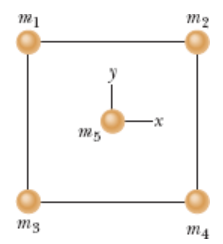
\includegraphics[width=0.3\textwidth]{fig/orp2l1q2.png}
\label{fig:ORP2q2}
\caption*{Fonte: \citeonline{Halliday2009vol2}}
\end{center}
\end{figure}

    \item[3.] \textbf{\cite{Halliday2009vol2}} A figura abaixo mostra duas cascas esféricas concêntricas homogêneas de massas $M_1$ e $M_2$. DEtermine o módulo da força gravitaconal a ue está sujeita uma partícula de massa $m$ situada a uma distância (a) $a$, (b) $b$ e (c) $c$ do centro comum das cascas.

\begin{figure}[H]
\begin{center}
\caption*{Desenho Questão 3.}
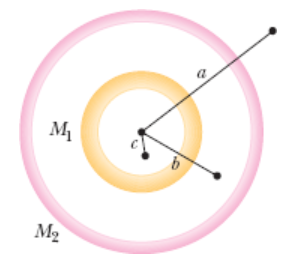
\includegraphics[width=0.3\textwidth]{fig/orp2l1q3.png}
\label{fig:ORP2q3}
\caption*{Fonte: \citeonline{Halliday2009vol2}}
\end{center}
\end{figure}

    \item[4.] \textbf{\cite{Halliday2009vol2}} Marte e a Terra tem diâmetros médios de $6,9 \times 10^3$ $km$ e $1,3 \times 10^4$ $km$, respectivamente. A massa de Marte é $0,11$ vezes a massa da Terra. Qual é a razão entre as massas específicas médias de Marte e da Terra? (b) Qual é o valor da aceleração gravitacional em Marte? (c) Qual é a velocidade de escape em Marte?

    \item[5.] \textbf{\cite{Halliday2009vol2}} Fobos, um satélite de Marte, se move em uma órbita aproximadamente circular com $9,4 \times 10^6$ $m$ de raio e um período de $7h39min$. Calcule a massa de Marte a partir dessas informações.

    \item[6.] \textbf{\cite{Halliday2009vol2}} A Figura abaixo mostra uma cavidade eférica no interior de uma esfera de chumbo de raio $R=4,00$ $cm$; a superfície da cavidade passa pelo centro dessa esfera e "toca" o lado direito da esfera. A massa da esfera antes de ser criada a cavidade era $M=2,95$ $kg$. Com que força gravitacional a esfera de chumbo com a cavidade atrai uma pequena esfera de massa $m=0,431$ $kg$ que está a uma distância $d=9,00$ $cm$ do centro da esfera de chumbo, na reta que passa pelo centro das duas esferas e pelo centro da cavidade?

\begin{figure}[H]
\begin{center}
\caption*{Desenho Questão 6.}
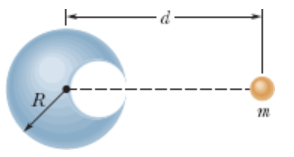
\includegraphics[width=0.3\textwidth]{fig/orp2l1q6.png}
\label{fig:ORP2q6}
\caption*{Fonte: \citeonline{Halliday2009vol2}}
\end{center}
\end{figure}

    \item[7.] \textbf{\cite{Halliday2009vol2}} Um planeta é modelado por um núcleo de raio $R$ e massa $M$ cercado por uma casca de raio interno $R$, raio externo $2R$ e massa $4M$. Se $M= 4,1 \times 10^{24}$ $kg$ e $R = 6,0 \times 10^6$ $m$, qual é a aceleração gravitacional de uma partícula em pontos situados a uma distância (a) $R$ e (b) $3R$ do centro do planeta?

    \item[8.] \textbf{\cite{Halliday2009vol2}} Zero, um planeta hipoético, tem massa de $5,0 \times 10^{23}$ $kg$, um raio de $3,0 \times 10^6$ $m$ e nenhuma atmosfera. Uma sonda espacial de $10$ $kg$ deve ser lançada verticalmente a partir da superfície. (a) Se a sonda for lançada com uma energia inicial de $5,0 \times 10^7$ $J$, qual será a energia cinética da sonda quando ela estiver a $4,0 \times 10^6$ $m$ do centro de Zero? (b) Com que energia cinética a sonda deverá ser lançada para atingir uma distância máxima de $8,0 \times 10^6$ $m$ em relação ao centro de Zero?

    \item[9.] \textbf{\cite{Halliday2009vol2}} Uma estrela de nêutrons típica tem massa igual à do So e raio de $10$ $km$. (a) Qual é a aceleração da gravidade na superfície da estrela? (b) COm que velocidade um objeto estaria se movendo se caísse a partir do repouso por uma distância de $1,0$ $m$ em direção à estrela? (Suponha que o movimento de rotação da estrela seja desprezível.)

    \item[10.] \textbf{\cite{Halliday2009vol2}} As massas e as coordenadas de três esferas são as seguintes: $20$ $kg$, $x = 0,50$ $m$, $y=1,0$ $m$; $40$ $kg$, $-1,0$ $m$, $y= -1,0$ $m$; $60$ $kg$, $x= 0$ $m$, $y= -0,5$ $m$. Qual é o módulo da força gravitacional que as três esferas exercem em uma esfera de $20$ $kg$ localizada na origem?

    \item[11.] \textbf{\cite{Halliday2009vol2}} Um objeto de massa $m$ é mantido inicialmente no lugar a uma distância $r=R_T$ do centro da Terra, em que $R_T$ é o raio da Terra. Seja $M_T$ a massa da Terra.  Uma força é aplicada ao objeto para deslocá-lo até uma distância $r=4R_T$, na qual é novamente mantido no lugar. Calcule, integrando o módulo da força, o trabalho realizado durante o deslocamento.

\end{itemize}
\newpage
\section{Lista 2 - ORP2} \label{ch:orp2l2}

\begin{itemize}
\item[1.] \textbf{\cite{Halliday2009vol2}} Uma janela de um escritório tem $3,4$ $m$ de largura por $2,1$ $m$ de altura. Como resultado da passagem de uma tempestade, a pressão do ar do lado de fora do edifício cai para $0,96 atm$, mas no interior do edifício permanece em $1,0$ $atm$. Qual é o módulo da força que empurra a janela por causa da diferença de pressão?


\item[2.] \textbf{\cite{Halliday2009vol2}} Calcule a diferença hidrostática entre a pressão arterial no cérebro e no pé de uma pessoa com $1,83$ $m$ de altura. A massa específica do sangue é $1,06 \times 10^3$ $kg/m^3$.


\item[3.] \textbf{\cite{Halliday2009vol2}} Um tanque cilíndrico de grande diâmetro está cheio d'água até uma profundidade $D  =0,30 $ $m$. Um furo de seção reta $A = 6,5$ $cm^2$ no fundo do tanque permite a drenagem da água. \textit{(a)} Qual é a velocidade de escoamento da água, em metros cúbicos por segundo? \textit{(b)} A que distância abaixo do fundo do tanque a seção reta do jorro é igual à metade da área do furo?


\item[4.] \textbf{\cite{Halliday2009vol2}} A água se move a uma velocidade de $5,0 m/s$ em um cano de seção reta $4,0$ $cm^2$. A água desce gradualmete $10 m$ enquanto a seção reta aumenta para $8,0$ $cm^2$. \textit{(a)} Qual é a velocidade da água depois da descida? \textit{(b)} Se a pressão antes da descida é $1,5 \times 10^5$ $Pa$, qual pe a pressão depois da descida?

\end{itemize}
\newpage
\section{Lista 3 - ORP2} \label{ch:orp2l3}

\begin{itemize}
\item[1.] \textbf{\cite{Halliday2009vol2}}Um oscilador pe formado por um bloco com uma massa de $0,500$ $kg$ ligado a uma mola. Quando é posto em oscilação com uma amplitude de $35,0$ $cm$ o oscilador repete o movimento a cada $0,500$ $s$. Determine (a) o período, (b) a frequência, (c) a frequência angular, (d) a constante elástica, (e) a velocidade máxima e (f) o módulo da força máxima que a mola exerce sobre o bloco.
\item[2.] \textbf{\cite{Halliday2009vol2}}Quando o deslocamento em um MHS é de metade da amplitude $x_m$, que fração da energia total é (a) energia cinética e (b) energia potencial? (c) Para que deslocamento, como fração da amplitude, a energia do sistema é metade da energia cinética e metade da energia potencial?
\item[3.] \textbf{\cite{Halliday2009vol2}}Um pêndulo físico é formado por uma régua de um metro, cujo ponto de suspensão é um pequeno furo feito na régua a uma distância $d$ da marca de $50$ $cm$. O período de oscilação é $2,5$ $s$. Determine o valor de $d$.
\item[4.] \textbf{\cite{Halliday2009vol2}}A amplitude de um oscilador fracamente amortecido diminui $3,0\%$ a cada ciclo. QUe porcentagem da energia mecânica do oscilador é perdida em cada ciclo?
\end{itemize}
\newpage
\section{Lista 4 - ORP2} \label{ch:orp2l4}

\begin{itemize}
\item[1.] \textbf{\cite{Halliday2009vol2}} Uma onda senoidal se propaga em uma corda. O tempo necessário para que um ponto da corda se desloque do deslocamento máximo até zero é $0,170$ $s$. (a) Qual é o período e (b) qual é a frequência da onda? (c) O comprimento de onda é $1,40$ $m$; qual é a velocidade da onda?

\item[2.] \textbf{\cite{Halliday2009vol2}} A massa específica de uma corda é $1,6 \times 10^{-4}$ $kg/m$. Uma onda transversal na corda é descrita pela equação
\begin{equation*}
y = (0,021mi)sin[(2,0 m^{-1})x + (30s^{-1})t].
\end{equation*}

(a) Qual é a velocidade da onda e (b) qual é a tração da corda?

\item[3.] \textbf{\cite{Halliday2009vol2}} Uma corda na qual ondas podem se propagar tem $2,70$ $m$ de comprimento e $260$ $g$ de massa. A tração da corda é $36,0$ $N$. Qual deve ser a frequência de ondas progressivas com uma amplitude de $7,70$ $mm$ para que a potência média seja $85,0$ $W$?

\item[4.] \textbf{\cite{Halliday2009vol2}} Duas ondas progressivas iguais, que se propagam no mesmo sentido, estão defasadas $\pi /2$  $rad$. Qual é a amplitude da onda resultante em tremo da amplitude comum $y_m$ das duas ondas?
\end{itemize}
\newpage
\section{Lista 5 - ORP2} \label{ch:orp2l5}

\begin{itemize}
\item[1.] \textbf{\cite{Halliday2009vol2}} Em que temperatura a leitura na escala Fahrenheit é igual (a) a duas vezes a leitura na escala Celcius e (b) metade da leitura na escala Celcius?

\item[2.] \textbf{\cite{Halliday2009vol2}} Um mastro de alumínio tem $33$ $m$ de altura. De quanto seu comprimento aumenta quando a temperatura aumenta de $15 $\textdegree$ C$?

\item[3.] \textbf{\cite{Halliday2009vol2}} Calcule a menor quantidade de energia, em joules, necessária para fundir $130$ $g$ de prata inicialmente a $15,0^{\circ}C$.

\item[4.] \textbf{\cite{Halliday2009vol2}} Uma esfera de $0,500$ $m$ de raio, cuja emissividade é $0,850$, está a $27,0^{\circ}C$ em um local onde a temperatura ambiente é $77,0^{\circ}C$. Com que taxa a esfera (a) emite e (b) absorve radiação térmica? (c) Qual é a taxa líquida de troca de energia da esfera?
\end{itemize}
\chapter{Aplicações da ORP 3} \label{apendice:orp3}
\section{Lista 1 - ORP3}\label{ch:orp3l1}
\begin{itemize}
    \item[1.] \textbf{\cite{halliday}} Um feixe de luz monocromática é absorvido por um filme fotográfico e fica registrado no filme. Um fóton é absorvido pelo filme se a energia do fóton for igual ou maior que a energia mínima de $0,6$ $eV$ necessária para desassociar uma molécula de AgBr do filme. (a) Qual é o maior comprimento de onda que pode ser registrado no filme? (b) A que região do espectro eletromagnético pertence esse comprimento de onda?

    \item[2.] \textbf{\cite{halliday}} (a) Qual é o momento, em $MeV/c$, de um fóton cuja energia é igual à energia de repouso de um elétron? Quais são (b) o comprimento de onda e (c) a frequência da radiação correspondente?

    \item[3.] \textbf{(\cite{halliday}/Adaptada)} A superfície do Sol se comporta aproximadamente como um corpo negro à temperatura de $5800$ $K$. (a) Calcule o comprimento de onda para o qual a radiância espectral da superfície do Sol é máxima e (b) indique em que região do espectro eletromagnético está esse comprimento deonda. (c) O universo se comporta aproximadamente como um corpo negro cuja radiação foi emitida quando os átomos se formaram pela primeira vez. Hoje em dia, o comprimento de onda para o qual a radiação desse corpo negro é máxima é $1,06$ $mm$ (um comprimento de onda que se encontra na faixa das micro-ondas). Qual é a temperatura atual do universo?

    \item[4.] \textbf{\cite{halliday}} No tubo de imagem de um velho aparelho de televisão, os elétrons são acelerados por uma diferença de potencial de $25,0$ $kV$. Qual é o comprimento de onda de de Broglie desses elétrons? (Não é necessário levar em conta efeitos relativísticos.)

    \item[5.] \textbf{\cite{halliday}} Mostre que o número de onda $k$ de uma partícula livre não relativística, de massa $m$, pode ser escrito na forma
    \begin{equation*}
        k = \frac{2 \pi \sqrt{2mK}}{h},
    \end{equation*}
    em que $K$ é a energia cinética da partícula.

    \item[6.] \textbf{\cite{halliday}} A indeterminação da posição de um elétron situado no eixo $x$ é $50$ $pm$, ou seja, um valor aproximadamente igual ao raio do átomo de hidrogênio. Qual é a menor indeterminação possível da componente $p$, do momento do elétron?

    \item[7.] \textbf{\cite{halliday}} (a) Um feixe de prótons de $5,0$ $eV$ incide em uma barreira de energia potencial de $6,0$ $eV$ de altura e $0,70$ $nm$ de largura, a uma taxa correspondente a uma corrente de $1000$ $A$. Quanto tempo é preciso esperar (em média) para que um próton atravesse a barreira? (b) QUanto tempo será preciso esperar, se o feixe contiver elétrons em vez de prótons?

    \item[8.] \textbf{\cite{halliday}} Um elétron está se movendo em uma região onde existe m potencial elétrico uniforme de $-200$ $V$ com uma enertgia (total) de $500$ $eV$. Determine (a) a energia cinética do elétron, em elétron-volts, (b) o momento do elétron, (c) a velocidade do elétron, (d) o coprimento de onda de de Broglie do elétron, (e) o número de onda do elétron.

    \item[9.] \textbf{\cite{halliday}} A resolução de um microscópio depende do comprimento de onda usado; o menor objeto que pode ser resolvido tem dimensões da oredem do comprimento de onda. Suponha que estamos interessados em "observar" o interior do átomo. Como um átomo tem um diâmetro da ordem de $100$ $pm$, isso significa que devemos ser capazes de resolver dimensões da ordem de $10$ $pm$. (a) Se um microscópio eletrônico for usado para este fim, qual deverá ser, no mínimo, a energia dos elétrons? (b) Se um microscópio ótico for usado, qual deverá ser, no mínimo,a energia dos fótons? (c) Qual dos dois microscópios parece ser mais prático? Por quê?

    \item[10.] \textbf{\cite{halliday}} Mostre que, se um fóton de energia $E$ for espalhado por um elétron livre em repouso,a energia cinética máxima do elétron espalhado será
    \begin{equation*}
        K_{max}= \frac{E^2}{E + mc^2/2}
    \end{equation*}
    
\end{itemize}
\newpage
\section{Lista 2 - ORP3} \label{ch:orp3l2}

\begin{itemize}
\item[1.] \textbf{\cite{Griffiths2011}} Demonstre que não há solução aceitável para a equação de Schrödinger (independente do tempo) para o poço quadrado infinito com $E = 0$ ou $E < 0$.

\item[2.] \textbf{\cite{Griffiths2011}} Uma partícula no potencial do oscilador harmônico está no estado
\begin{equation*}
\Psi (x,0) = A[3{\psi}_0 (x) + 4{\psi}_1(x)]
\end{equation*}
(a) Calcule A. 
\par
(b) Monte $\psi(x,t)$ e $|\psi(x,t)|^2$.
\par 
(c) Calcule $\langle x \rangle$ e $\langle p \rangle$.
\par 
(d) Ao medir a energia da partícula, que valores você poderá obter e quais as probabilidades de obter cada um deles?

\item[3.]\textbf{\cite{Griffiths2011}} Uma partícula livre tem a seguinte função de onda inicial:
\begin{equation*}
\Psi (x,0) = A e^{-a|x|},
\end{equation*}
em que $A$ e $a$ são constantes reais positivas.
\par 
(a) Normalize $\Psi(x,0)$.
\par 
(b) Calcule $\phi (k)$.
\par 
(c) Monte $\Psi (x,t)$ na forma integral.
\par 
(d) Discuta os casos limites ($a$ muito grande ou muito pequeno).

\end{itemize}
\newpage
\section{Lista 3 - ORP3} \label{ch:orp3l3}

\begin{itemize}
    \item[1.] \textbf{\cite{Griffiths2011}/Adaptada} 
    \begin{itemize}
        \item[a)] Resolva todas as \textbf{relações de comutação canônicas} para os componenetes dos operadores \textbf{r} e \textbf{p}: $[x,y]$, $[x,p_y]$, $[x,p_x]$, $[x,p_z]$, e assim por diante. \textit{Resposta}:
        \begin{center}
            $[r_i,p_j]=-[p_i,r_j]=i \hbar \delta_{ij}$, $[r_i,r_j]=[p_i,p_j]=0$,
        \end{center}
        em que os índices representam $x$, $y$ ou $z$, e $r_x=x$, $r_y=y$ e $r_z=z$.

        \item[b)] Confirme o teorema de Ehrenfes para três dimensões:
        \begin{center}
            $\frac{d}{dt} \langle \textbf{r} \rangle = \frac{1}{m} \langle \textbf{p} \rangle$ e $\frac{d}{dt}\langle \textbf{p} \rangle = \langle - \nabla V \rangle.$
        \end{center}

        \item[c)] Formule o princípio da incerteza de Heisenberg em três dimensões. \textit{Resposta}:
        \begin{center}
            $\sigma_x \sigma_{p_x} \geq \frac{\hbar}{2}$, $\sigma_y \sigma_{p_y} \geq \frac{\hbar}{2}$, $\sigma_z \sigma_{p_z} \geq \frac{\hbar}{2}$,
        \end{center}
        mas vamos dizer que não haja restrição em $\sigma_x \sigma_{p_y}$.
    \end{itemize}

    \item[2.] \textbf{\cite{Griffiths2011}/Adaptada} Utiliza as Equações abaixo para montar $Y^{0}_{0}$ e $Y^{1}_{2}$. Certifique-se de que eles estejam normalizados e sejam ortogonais.

    \begin{equation*}
        P^{m}_{l}(x) \equiv (1-x^2)^{|m|/2}\left( \frac{d}{dx} \right)^{|m|}P_{l}(x)
    \end{equation*}
    \begin{equation*}
        P_{l}(x) \equiv \frac{1}{2^l l!}\left( \frac{d}{dx} \right)^l (x^2-1)^l
    \end{equation*}
    \begin{equation*}
        Y^{m}_{l}(\theta,\phi) = \epsilon\sqrt{\frac{(2l+1)}{2 \pi}\frac{(l-|m|)!}{(l+|m|)!}}e^{im\phi}P^{m}_{l}( \cos \theta)
    \end{equation*} 
\end{itemize}
\chapter{MODELO FOLHA ASA} \label{ch:modeloASA}
\begin{figure*}[htb]
  \centering
  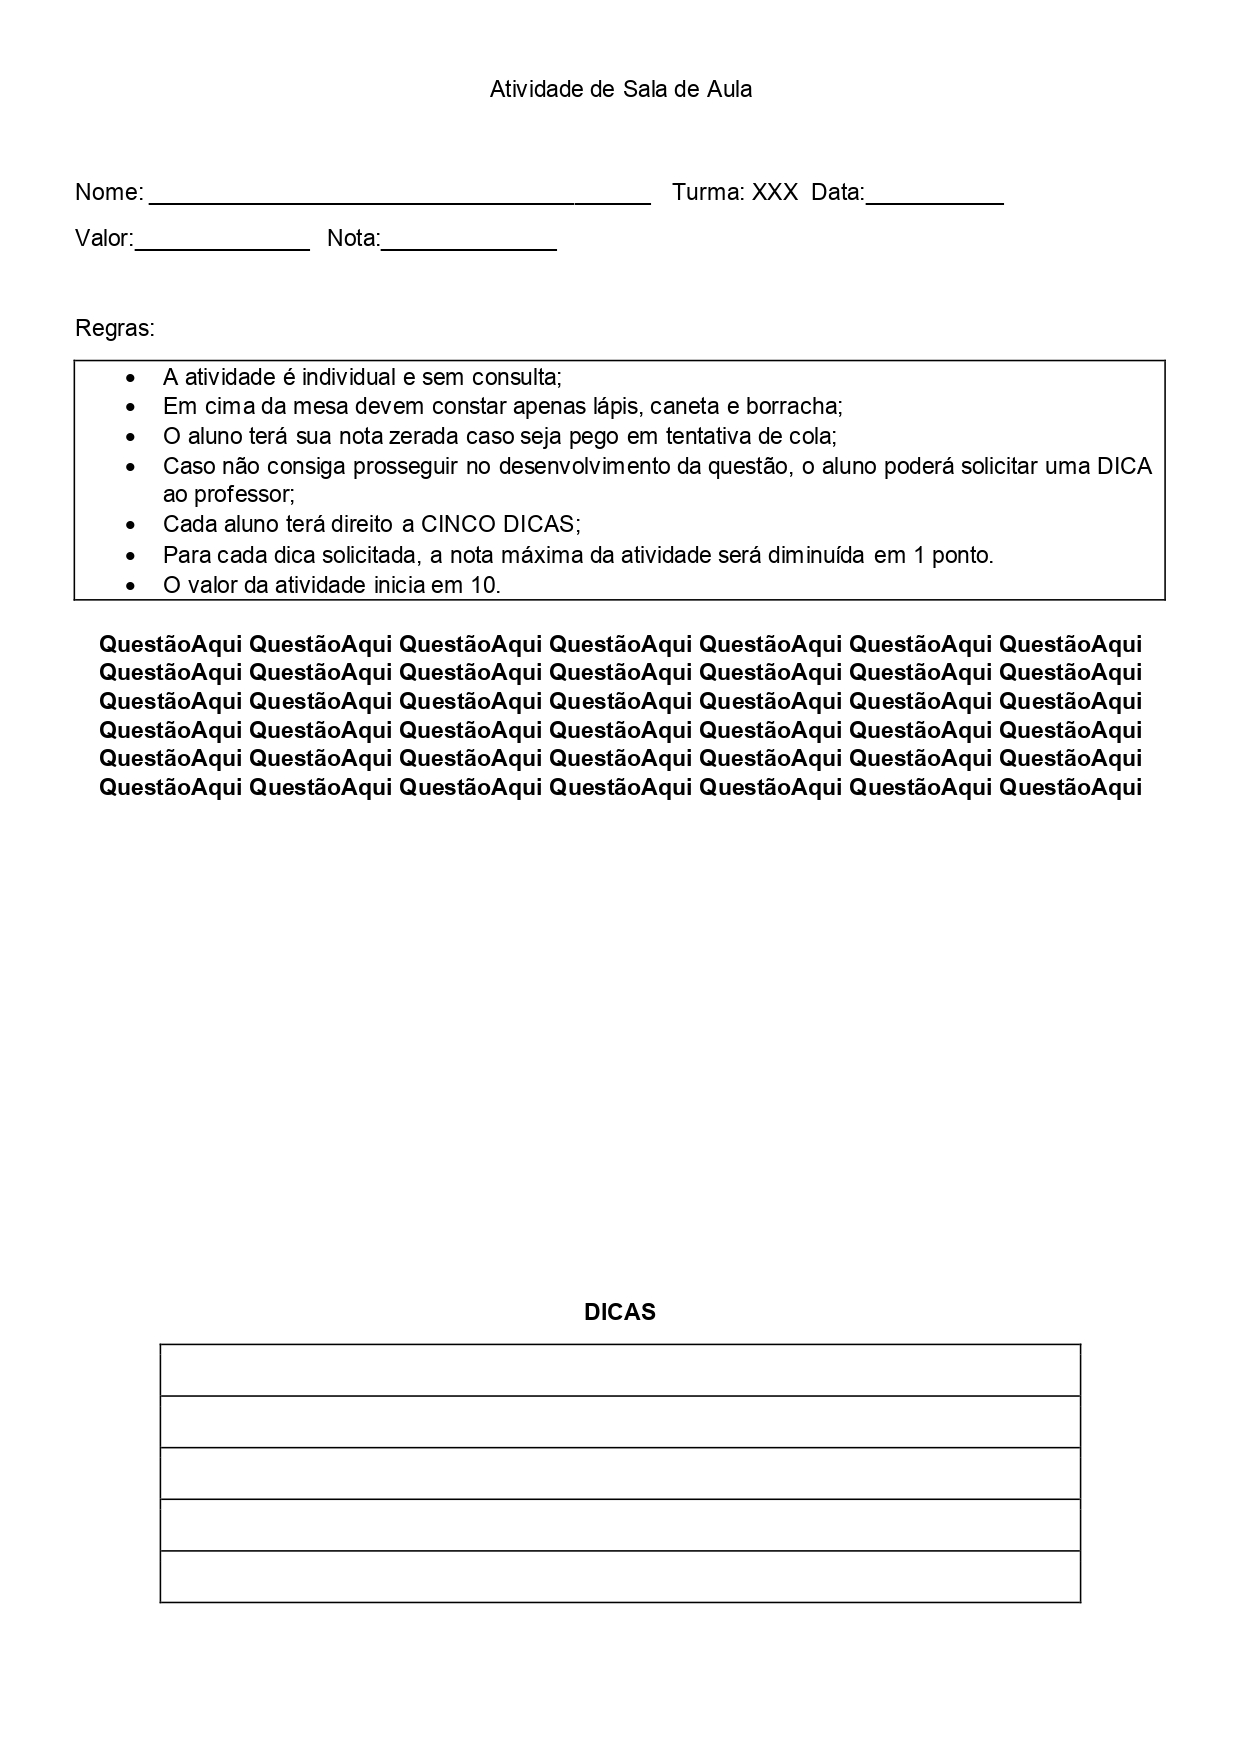
\includegraphics[width=0.9\textwidth]{fig/modeloASA_pages-to-jpg-0001.jpg}
  \caption{Modelo de folha utilizado na aplicação das ASA}
  \label{fig:figura}
\end{figure*}
\chapter{ASA 1} \label{apendice:asa1}
\section{Aplicação 1} \label{ch:ASA1a1}
\begin{itemize}
    \item[Modelo A:] Calcule a velocidade média nos dois casos a seguir:
    \begin{itemize}
        \item[(a)] Você caminha $73,2$ $m$ a uma velocidade de $1,22$ $m/s$ e depois corre $73,2$ $m$ a $3,05$ $m/s$ em uma pista reta.
        \item[(b)] Você caminha $1,00$ $min$ com velocidade de $1,22$ $m/s$ e depois corre por $1,00$ $min$ a $3,05$ $m/s$ em uma pista reta.
    \end{itemize}
    \item[Modelo B:] Calcule a velocidade média nos dois casos a seguir:
    \begin{itemize}
        \item[(a)] Você caminha $75,2$ $m$ a uma velocidade de $1,26$ $m/s$ e depois corre $73,2$ $m$ a $3,05$ $m/s$ em uma pista reta.
        \item[(b)] Você caminha $1,00$ $min$ com velocidade de $1,22$ $m/s$ e depois corre por $1,00$ $min$ a $3,15$ $m/s$ em uma pista reta.
    \end{itemize}
    \item[Modelo C:] Calcule a velocidade média nos dois casos a seguir:
    \begin{itemize}
        \item[(a)] Você caminha $73,2$ $m$ a uma velocidade de $1,22$ $m/s$ e depois corre $73,2$ $m$ a $3,05$ $m/s$ em uma pista reta.
        \item[(b)] Você caminha $1,00$ $min$ com velocidade de $1,22$ $m/s$ e depois corre por $1,50$ $min$ a $3,25$ $m/s$ em uma pista reta.
    \end{itemize}
    \item[Modelo D:] Calcule a velocidade média nos dois casos a seguir:
    \begin{itemize}
        \item[(a)] Você caminha $79,2$ $m$ a uma velocidade de $1,36$ $m/s$ e depois corre $74,2$ $m$ a $3,05$ $m/s$ em uma pista reta.
        \item[(b)] Você caminha $1,00$ $min$ com velocidade de $1,22$ $m/s$ e depois corre por $2,00$ $min$ a $3,05$ $m/s$ em uma pista reta.
    \end{itemize}
\end{itemize}
\newpage
\section{Aplicação 2}\label{ch:ASA1a2}
\begin{itemize}
    \item[Modelo A:] Um trem de $150$ $m$ de comprimento se desloca com velocidade esalar constante de $57,6$ $km/h$. Esse trem atravessa um túnel e leva $50$ $s$ desde a entrada até a saída completa dentro dele. Qual é o comprimento total do túnel?
    
    \item[Modelo B:] Um trem de $200$ $m$ de comprimento se desloca com velocidade esalar constante de $50,4$ $km/h$. Esse trem atravessa um túnel e leva $40$ $s$ desde a entrada até a saída completa dentro dele. Qual é o comprimento total do túnel?
    
    \item[Modelo C:] Um trem de $100$ $m$ de comprimento se desloca com velocidade esalar constante de $61,2$ $km/h$. Esse trem atravessa um túnel e leva $120$ $s$ desde a entrada até a saída completa dentro dele. Qual é o comprimento total do túnel?
    
    \item[Modelo D:] Um trem de $75$ $m$ de comprimento se desloca com velocidade esalar constante de $57,6$ $km/h$. Esse trem atravessa um túnel e leva $240$ $s$ desde a entrada até a saída completa dentro dele. Qual é o comprimento total do túnel?
\end{itemize}
\newpage
\section{Aplicação 3} \label{ch:ASA1a3}
\begin{itemize}
    \item[Modelo A:] Em uma fase de testes para fazer entregas rápidas, um \textit{drone}, parado sobre local de entrega, deixa cair um pacote de uma altura de $150$ $m$ acima do solo. Desconsiderando os efeitos de resistência do ar e considerando $g=10$ $m/s^2$, determine (a) o tempo que o pacote leva para atingir o solo e (b) a velocidade do pacote ao atingir o solo.
    
    \item[Modelo B:] Em uma fase de testes para fazer entregas rápidas, um \textit{drone}, parado sobre local de entrega, deixa cair um pacote de uma altura de $160$ $m$ acima do solo. Desconsiderando os efeitos de resistência do ar e considerando $g=10$ $m/s^2$, determine (a) o tempo que o pacote leva para atingir o solo e (b) a velocidade do pacote ao atingir o solo.
    
    \item[Modelo C:] Em uma fase de testes para fazer entregas rápidas, um \textit{drone}, parado sobre local de entrega, deixa cair um pacote de uma altura de $181$ $m$ acima do solo. Desconsiderando os efeitos de resistência do ar e considerando $g=10$ $m/s^2$, determine (a) o tempo que o pacote leva para atingir o solo e (b) a velocidade do pacote ao atingir o solo.
    
    \item[Modelo D:] Em uma fase de testes para fazer entregas rápidas, um \textit{drone}, parado sobre local de entrega, deixa cair um pacote de uma altura de $175$ $m$ acima do solo. Desconsiderando os efeitos de resistência do ar e considerando $g=10$ $m/s^2$, determine (a) o tempo que o pacote leva para atingir o solo e (b) a velocidade do pacote ao atingir o solo.
    
\end{itemize}


\chapter{ASA 2} \label{apendice:asa2}
\section{Aplicação 1} \label{ch:ASA2a1}

\begin{itemize}
    \item[Modelo A:] Em uma escala linear $X$, a água congela a $-125,0^{\circ}X$ e evapora a $375,0^{\circ}X$. Em uma escala linear de temperatura $Y$, a água congela a $-70,0^{\circ}Y$ e evapora a $-30,0^{\circ}Y$. Uma temperatura de $50,0^{\circ}Y$ corresponde a que temperatura na escala $X$?    

    \item[Modelo B:] Em uma escala linear $X$, a água congela a $-120,0^{\circ}X$ e evapora a $375,0^{\circ}X$. Em uma escala linear de temperatura $Y$, a água congela a $-70,0^{\circ}Y$ e evapora a $-30,0^{\circ}Y$. Uma temperatura de $50,5^{\circ}Y$ corresponde a que temperatura na escala $X$? 
   
    \item[Modelo C:] Em uma escala linear $X$, a água congela a $-125,0^{\circ}X$ e evapora a $380,0^{\circ}X$. Em uma escala linear de temperatura $Y$, a água congela a $-70,0^{\circ}Y$ e evapora a $-30,0^{\circ}Y$. Uma temperatura de $60,0^{\circ}Y$ corresponde a que temperatura na escala $X$? 
    
    \item[Modelo D:] Em uma escala linear $X$, a água congela a $-122,0^{\circ}X$ e evapora a $372,0^{\circ}X$. Em uma escala linear de temperatura $Y$, a água congela a $-70,0^{\circ}Y$ e evapora a $-30,0^{\circ}Y$. Uma temperatura de $60,5^{\circ}Y$ corresponde a que temperatura na escala $X$? 

    \end{itemize}
\newpage

\section{Aplicação 2} \label{ch:ASA2a2}
\begin{itemize}
    \item[Modelo A:] Calcule a quantidade de calor necessário para tranformar $200$ $g$ de gelo a $-5^{\circ}C$ em vapor de água a $107^{\circ}C$.
    
    \item[Modelo B:] Calcule a quantidade de calor necessário para tranformar $300$ $g$ de gelo a $-10^{\circ}C$ em vapor de água a $110^{\circ}C$.
    
    \item[Modelo C:] Calcule a quantidade de calor necessário para tranformar $100$ $g$ de gelo a $-15^{\circ}C$ em vapor de água a $120^{\circ}C$.
    
    \item[Modelo D:] Calcule a quantidade de calor necessário para tranformar $500$ $g$ de gelo a $-25^{\circ}C$ em vapor de água a $117^{\circ}C$.
    
\end{itemize}
Dados fornecidos em todos os modelos:
\begin{itemize}
    \item $c_{gelo} = 0,5 cal/g^{\circ}C$;
    \item $c_{agua} = 1 cal/g^{\circ}C$;
    \item $c_{gelo} = 0,40 cal/g^{\circ}C$;
    \item $L_{fusao} = 80 cal/g$;
    \item $L_{ebulicao} = 540 cal/g$.
\end{itemize}
\newpage

\section{Aplicação 3} \label{ch:ASA2a3}
\begin{itemize}
    \item[Modelo A:] Em uma fábrica usa-se uma barra de alumínio de $80$ $cm^2$ de seção reta e $20$ $cm$ de comprimento, para manter constante a temperatura da máquina em operação. Uma das extremidades da barra é colocada em contato com a máquina que opera à temperatura constante de $400^{\circ}C$, enquanto a outra extremidade está em contato com uma barra de gelo na sua temperatura de fusão. Sabendo-se que o calor latente de fusão do gelo é de $80$ $cal/g$, que o coeficiente de condutibilidade térmica do alumínio é de $0,5$ $cal/s \cdot cm \cdot ^{\circ}C$ e desprezando-se as trocas de calor do sistema máquina-gelo com o ambiente, calcule o tempo necessário para derreter $500$ $g$ de gelo.
    
    \item[Modelo B:] Em uma fábrica usa-se uma barra de alumínio de $60$ $cm^2$ de seção reta e $40$ $cm$ de comprimento, para manter constante a temperatura da máquina em operação. Uma das extremidades da barra é colocada em contato com a máquina que opera à temperatura constante de $400^{\circ}C$, enquanto a outra extremidade está em contato com uma barra de gelo na sua temperatura de fusão. Sabendo-se que o calor latente de fusão do gelo é de $80$ $cal/g$, que o coeficiente de condutibilidade térmica do alumínio é de $0,5$ $cal/s \cdot cm \cdot ^{\circ}C$ e desprezando-se as trocas de calor do sistema máquina-gelo com o ambiente, calcule o tempo necessário para derreter $100$ $g$ de gelo.
    
    \item[Modelo C:] Em uma fábrica usa-se uma barra de alumínio de $80$ $cm^2$ de seção reta e $30$ $cm$ de comprimento, para manter constante a temperatura da máquina em operação. Uma das extremidades da barra é colocada em contato com a máquina que opera à temperatura constante de $400^{\circ}C$, enquanto a outra extremidade está em contato com uma barra de gelo na sua temperatura de fusão. Sabendo-se que o calor latente de fusão do gelo é de $80$ $cal/g$, que o coeficiente de condutibilidade térmica do alumínio é de $0,5$ $cal/s \cdot cm \cdot ^{\circ}C$ e desprezando-se as trocas de calor do sistema máquina-gelo com o ambiente, calcule o tempo necessário para derreter $200$ $g$ de gelo.
    
    \item[Modelo D:] Em uma fábrica usa-se uma barra de alumínio de $100$ $cm^2$ de seção reta e $10$ $cm$ de comprimento, para manter constante a temperatura da máquina em operação. Uma das extremidades da barra é colocada em contato com a máquina que opera à temperatura constante de $400^{\circ}C$, enquanto a outra extremidade está em contato com uma barra de gelo na sua temperatura de fusão. Sabendo-se que o calor latente de fusão do gelo é de $80$ $cal/g$, que o coeficiente de condutibilidade térmica do alumínio é de $0,5$ $cal/s \cdot cm \cdot ^{\circ}C$ e desprezando-se as trocas de calor do sistema máquina-gelo com o ambiente, calcule o tempo necessário para derreter $1000$ $g$ de gelo.
    
\end{itemize}
\chapter{ASA 3} \label{apendice:asa3}
\section{Aplicação 1} \label{ch:ASA3a1}

\begin{itemize}
    \item[Modelo A:] Deseja-se utilizar um objeto metálico, inicialmente neutro, pelos processos de eletrização conhecidos, e obter uma quantidade de carga negativa $3,2$ $\mu C$. Será necessário acrescentar ou retirar elétrons? Quantos elétrons serão necessários? 
    
    \item[Modelo B:] Deseja-se utilizar um objeto metálico, inicialmente neutro, pelos processos de eletrização conhecidos, e obter uma quantidade de carga negativa $16,0$ $\mu C$. Será necessário acrescentar ou retirar elétrons? Quantos elétrons serão necessários? 
   
    \item[Modelo C:] Deseja-se utilizar um objeto metálico, inicialmente neutro, pelos processos de eletrização conhecidos, e obter uma quantidade de carga negativa $12,8$ $\mu C$. Será necessário acrescentar ou retirar elétrons? Quantos elétrons serão necessários? 
    
    \item[Modelo D:] Deseja-se utilizar um objeto metálico, inicialmente neutro, pelos processos de eletrização conhecidos, e obter uma quantidade de carga negativa $6,4$ $\mu C$. Será necessário acrescentar ou retirar elétrons? Quantos elétrons serão necessários? 

\end{itemize}
\newpage
\section{Aplicação 2} \label{ch:ASA3a2}
\begin{itemize}
    \item[Modelo A:] Duas cargas puntiformes, $Q_1 = 2$ $\mu C$ e $Q_2 = -6$ $\mu C$, estão fixas e separadas por uma distância de $600$ $nm$ no vácuo. Uma terceira carga $Q_3 = 3$ $\mu C$ é colocada no ponto médio do segmento que une as cargas $Q_1$ e $Q_2$. Qual o módulo da força elétrica resultante da carga $Q_3$? Qual a direção e o sentido desta força resultante?
    
    \item[Modelo B:] Duas cargas puntiformes, $Q_1 = 4$ $\mu C$ e $Q_2 = -5$ $\mu C$, estão fixas e separadas por uma distância de $600$ $nm$ no vácuo. Uma terceira carga $Q_3 = 1$ $\mu C$ é colocada no ponto médio do segmento que une as cargas $Q_1$ e $Q_2$. Qual o módulo da força elétrica resultante da carga $Q_3$? Qual a direção e o sentido desta força resultante?
    
    \item[Modelo C:] Duas cargas puntiformes, $Q_1 = 2$ $\mu C$ e $Q_2 = -6$ $\mu C$, estão fixas e separadas por uma distância de $800$ $nm$ no vácuo. Uma terceira carga $Q_3 = 2$ $\mu C$ é colocada no ponto médio do segmento que une as cargas $Q_1$ e $Q_2$. Qual o módulo da força elétrica resultante da carga $Q_3$? Qual a direção e o sentido desta força resultante?
    
    \item[Modelo D:] Duas cargas puntiformes, $Q_1 = 9$ $\mu C$ e $Q_2 = -6$ $\mu C$, estão fixas e separadas por uma distância de $300$ $nm$ no vácuo. Uma terceira carga $Q_3 = 8$ $\mu C$ é colocada no ponto médio do segmento que une as cargas $Q_1$ e $Q_2$. Qual o módulo da força elétrica resultante da carga $Q_3$? Qual a direção e o sentido desta força resultante?
    
\end{itemize}
\newpage
\section{Aplicação 3} \label{ch:ASA3a3}
\begin{itemize}
    \item[Modelo A:] Admita que a distância entre os eletrodos de um campo elétrico é de $20$ $cm$ e que a diferença de potencial efetia aplicada ao circuito é de $6$ $V$. Calcule (a) a intensidade do campo elétrico (em $V/m$) e (b) a força elétrica exercida por ese campo em uma partícula de carga $e$.
    
    \item[Modelo B:] Admita que a distância entre os eletrodos de um campo elétrico é de $50$ $cm$ e que a diferença de potencial efetia aplicada ao circuito é de $8$ $V$. Calcule (a) a intensidade do campo elétrico (em $V/m$) e (b) a força elétrica exercida por ese campo em uma partícula de carga $3e$.
    
    \item[Modelo C:] Admita que a distância entre os eletrodos de um campo elétrico é de $40$ $cm$ e que a diferença de potencial efetia aplicada ao circuito é de $6$ $V$. Calcule (a) a intensidade do campo elétrico (em $V/m$) e (b) a força elétrica exercida por ese campo em uma partícula de carga $3e$.
    
    \item[Modelo D:] Admita que a distância entre os eletrodos de um campo elétrico é de $20$ $cm$ e que a diferença de potencial efetia aplicada ao circuito é de $12$ $V$. Calcule (a) a intensidade do campo elétrico (em $V/m$) e (b) a força elétrica exercida por ese campo em uma partícula de carga $2e$.
    
\end{itemize}
\chapter{QUESTIONÁRIO FINAL - PÓS ASA} \label{ch:questASA}

\begin{center}
    \textbf{ATIVIDADES DE SALA DE AULA}
\end{center}

Este formulário é anônimo, ou seja, nenhum dado pessoal de vocês será transmitido para mim. Podem responder com sinceridade.

Conto com a colaboração de todos.

\begin{itemize}
    \item Qual sua turma:
    \begin{itemize}
        \item[$\circ$] 101
        \item[$\circ$] 201
        \item[$\circ$] 301
        
    \end{itemize}

    \item[1.] Sinto que os problemas presentes nas Atividades de Sala de Aula possuíam um grau de dificuldade similar aos problemas presentes no livro e nos realizados em sala de aula. \label{item:qasa1}
    \vspace{0.75cm}
    
    \begin{minipage}{\linewidth}
    \centering
    \begin{tabular}{|c|c|c|c|c|}
    \hline
    \textbf{1} & \textbf{2} & \textbf{3} & \textbf{4} & \textbf{5} \\
    \hline
    Discordo totalmente & \phantom{aaaaaaaa} & \phantom{aaaaaaaa} & \phantom{aaaaaaaa} & Concordo totalmente \\
    \hline
    \end{tabular}
    \end{minipage}
 
    \item[2.] Sinto que as Atividades de Sala de Aula são uma boa maneira de verificar meus conhecimentos e aprendizagens de Física.
    \vspace{0.75cm}
    
    \begin{minipage}{\linewidth}
    \centering
    \begin{tabular}{|c|c|c|c|c|}
    \hline
    \textbf{1} & \textbf{2} & \textbf{3} & \textbf{4} & \textbf{5} \\
    \hline
    Discordo totalmente & \phantom{aaaaaaaa} & \phantom{aaaaaaaa} & \phantom{aaaaaaaa} & Concordo totalmente \\
    \hline
    \end{tabular}
    \end{minipage}

    \item[3.] Sinto que as dicas presentes nas Atividades de Sala de Aula podem me auxiliar a resolver o problema quando não consigo prosseguir.
    \vspace{0.75cm}
    
    \begin{minipage}{\linewidth}
    \centering
    \begin{tabular}{|c|c|c|c|c|}
    \hline
    \textbf{1} & \textbf{2} & \textbf{3} & \textbf{4} & \textbf{5} \\
    \hline
    Discordo totalmente & \phantom{aaaaaaaa} & \phantom{aaaaaaaa} & \phantom{aaaaaaaa} & Concordo totalmente \\
    \hline
    \end{tabular}
    \end{minipage}

    \item[4.] Sinto que consigo entender melhor minhas dificuldades após a realização das Atividades de Sala de Aula.
    \vspace{0.75cm}
    
    \begin{minipage}{\linewidth}
    \centering
    \begin{tabular}{|c|c|c|c|c|}
    \hline
    \textbf{1} & \textbf{2} & \textbf{3} & \textbf{4} & \textbf{5} \\
    \hline
    Discordo totalmente & \phantom{aaaaaaaa} & \phantom{aaaaaaaa} & \phantom{aaaaaaaa} & Concordo totalmente \\
    \hline
    \end{tabular}
    \end{minipage}
\newline\newline\newline
    \item[5.] Considero que o número de Atividades de Sala de Aula poderia ser maior ao longo do trimestre.
    \vspace{0.75cm}
    
    \begin{minipage}{\linewidth}
    \centering
    \begin{tabular}{|c|c|c|c|c|}
    \hline
    \textbf{1} & \textbf{2} & \textbf{3} & \textbf{4} & \textbf{5} \\
    \hline
    Discordo totalmente & \phantom{aaaaaaaa} & \phantom{aaaaaaaa} & \phantom{aaaaaaaa} & Concordo totalmente \\
    \hline
    \end{tabular}
    \end{minipage}
\end{itemize}

\begin{table}[ht]
\captionsetup{justification=centering, labelsep=newline} % Centralize a legenda horizontalmente e adicione uma nova linha após o rótulo
\begin{tabularx}{\linewidth}{|>{\centering\arraybackslash}X|}
\hline
\textbf{Escreva toda e qualquer observação e/ou reclamação a respeito das Atividades de Sala de Aula aqui.}  \\
\hline
\rule{\dimexpr\linewidth-2\tabcolsep}{0.4pt} \\
\rule{\dimexpr\linewidth-2\tabcolsep}{0.4pt} \\
\rule{\dimexpr\linewidth-2\tabcolsep}{0.4pt} \\
\rule{\dimexpr\linewidth-2\tabcolsep}{0.4pt} \\
\rule{\dimexpr\linewidth-2\tabcolsep}{0.4pt} \\
\hline
\end{tabularx}

\end{table}


\end{apendicesenv}
%
\end{document}
